\documentclass{multi}


\title{Differentiability, chain rule, directional derivatives, gradient}
\course{Math 60: Multivariable Calculus}
\date{2017 September 4 (Monday)}


\tdplotsetmaincoords{60}{120}

\begin{document}

%\section*{Differentiable Functions, Chain Rule, Directional Derivative, Relations to Gradient}

%A multivariable function \(f\) is said to be differentiable at \((a, b)\) 

\section*{Differentiability} 

A multivariable function \(\vec f\colon \mathbb R^n \to \mathbb R^m\) is said to be differentiable at \(\vec a \in \mathbb R^n\) if all its partial derivatives \(\frac{\partial \vec f}{\partial x_i}\) exist \emph{and} the local tangent plane \(\vec h(\vec x) = \vec f(\vec a) + \nabla \vec f(\vec a) \cdot (\vec x - \vec a)\) is a ``good'' approximation of the function:
\[
    \lim_{\vec x \to \vec a} = \frac{\vec f(\vec x) - \vec h(\vec x)}{|\vec x - \vec a|} = 0.
\]

A nice little shortcut, because we're college math students and not hardcore real analysts, is that a function is differentiable if its partial derivatives are all continuous.

\section*{Chain Rule}

The chain rule deals with the \emph{composition} of two functions. In one-variable calculus, the chain rule looks something like, for some function \(f = g \circ h\) (that is, \(f(x) = g(h(x))\)),
\[
    \frac{\mathrm df}{\mathrm dx} = \frac{\mathrm df}{\mathrm dh} \frac{\mathrm dh}{\mathrm dx} = \frac{\mathrm dg}{\mathrm dh} \frac{\mathrm dh}{\mathrm dx} = g'(h(x)) h'(x).
\]

For multi-variable functions (\(D\), the chain rule takes on a matrix form:
\[
    D (\vec g \circ \vec h) = D (\vec g) D (\vec h).
\]

\paragraph{Example}

Consider \(\vec f\colon \mathbb R^3 \to \mathbb R^2\) given by 
\[
    \vec f(x_1, x_2, x_3) = (x_1 - x_2, x_1 x_2 x_3),
\]
and \(\vec x\colon \mathbb R^2 \to \mathbb R^3\) given by
\[
    \vec x(t_1, t_2) = (t_1 t_2, t_1^2, t_2^2).
\]

\paragraph{Context}

Here's how the mapping looks:
\[
    \mathbb R^2 \overset{\vec x}{\to} \mathbb R^3 \overset{\vec f}{\to} \mathbb R^2,
\]
or
\[
    (t_1, t_2) 
    \overset{\vec x}{\mapsto} 
    (\underbrace{x_1(t_1, t_2)}_{t_1 t_2}, 
     \underbrace{x_2(t_1, t_2)}_{t_1^2}, 
     \underbrace{x_3(t_1, t_2)}_{t_2^2})
    \overset{\vec f}{\mapsto}
    (\underbrace{f_1(x_1, x_2, x_3)}_{x_1-x_2}, 
     \underbrace{f_2(x_1, x_2, x_3)}_{x_1 x_2 x_3}).
\]

Notice the overall (composed) mapping is then
\[
    \mathbb R^2 \xrightarrow{\vec f \circ \vec x} \mathbb R^2.
\]

\paragraph{Solution (method 1): tedious substitution}

Find the derivative of the composition of \(f\) and \(x\),
\[
    D(\vec f \circ \vec x)(\vec t).
\]

We can simply plug in the composed function 
\[
    (\vec f \circ \vec x)(\vec t) = (x_1-x_2, x_1 x_2 x_3) = (t_1 t_2 - t_1^2, (t_1 t_2) (t_1^2) (t_2^2)) = (t_1 t_2 - t_1^2, t_1^3 t_2^3)
\]
and take the derivative:
\[
    D(\vec f \circ \vec x)(\vec t) = 
    \begin{pmatrix}
        \partial_{t_1} \left(t_1 t_2 - t_1^2\right) & \partial_{t_2} \left(t_1 t_2 - t_1^2\right) \\
        \partial_{t_1} \left(t_1^3 t_2^3\right) & \partial_{t_2} \left(t_1^3 t_2^3\right)
    \end{pmatrix} =
    \begin{pmatrix}
        t_2 - 2 t_1 & t_1 \\
        3 t_1^2 t_2^3 & 3 t_1^3 t_2^2
    \end{pmatrix}.
\]

\paragraph{Solution (method 2): chain rule (\emph{better!!!})}

Alternatively, apply the chain rule:
\begin{align*}
    D(\vec f \circ \vec x)(\vec t) &= D\vec f(\vec x) D\vec x(\vec t) \\
        &=
        \begin{pmatrix}
            \partial_{x_1} (x_1 - x_2) & \partial_{x_2} (x_1 - x_2) & \partial_{x_3} (x_1 - x_2) \\
            \partial_{x_1} (x_1 x_2 x_3) & \partial_{x_2} (x_1 x_2 x_3) & \partial_{x_3} (x_1 x_2 x_3) \\
        \end{pmatrix}
        \begin{pmatrix}
            \partial_{t_1} (t_1 t_2) & \partial_{t_2} (t_1 t_2) \\
            \partial_{t_1} (t_1^2) & \partial_{t_2} (t_1^2) \\
            \partial_{t_1} (t_2^2) & \partial_{t_2} (t_2^2)
        \end{pmatrix} \\
        &=
        \begin{pmatrix}
            1 & -1 & 0 \\
            x_2 x_3 & x_1 x_3 & x_1 x_2
        \end{pmatrix}
        \begin{pmatrix}
            t_2 & t_1 \\
            2 t_1 & 0 \\
            0 & 2 t_2
        \end{pmatrix} \\
        &= 
        \begin{pmatrix}
            t_2 - 2 t_1 & t_1 \\
            x_2 x_3 t_2 + 2 x_1 x_3 t_1 & x_2 x_3 t_1 + 2 x_1 x_2 t_2
        \end{pmatrix} \\
        &=
        \begin{pmatrix}
            t_2 - 2 t_1 & t_1 \\
            (t_1^2) (t_2^2) t_2 + 2 (t_1 t_2) (t_2^2) t_1 & (t_1^2) (t_2^2) t_1 + 2 (t_1 t_2) (t_1^2) t_2
        \end{pmatrix} \\
        &=
        \begin{pmatrix}
            t_2 - 2 t_1 & t_1 \\
            3 t_1^2 t_2^3 & 3 t_1^3 t_2^2
        \end{pmatrix}.
\end{align*}


\paragraph{Solution (method 3?): cool diagrams}

\begin{center}
    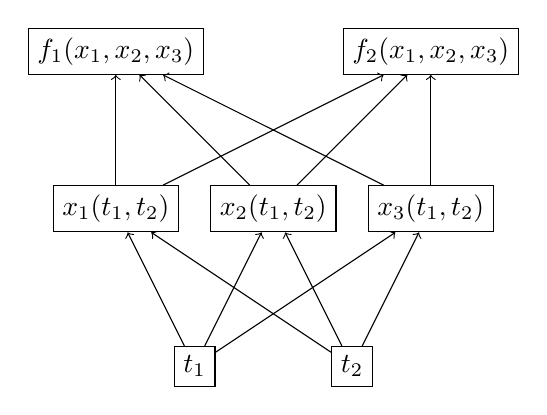
\begin{tikzpicture}
        

\path
    (-2, 0) node[draw](f1) {\(f_1(x_1, x_2, x_3)\)}
    ( 2, 0) node[draw](f2) {\(f_2(x_1, x_2, x_3)\)}
    (-2,-2) node[draw](x1){\(x_1(t_1, t_2)\)}
    ( 0,-2) node[draw](x2){\(x_2(t_1, t_2)\)}
    ( 2,-2) node[draw](x3){\(x_3(t_1, t_2)\)}
    (-1,-4) node[draw](t1){\(t_1\)}
    ( 1,-4) node[draw](t2){\(t_2\)}
;

\path[draw, <-] 
    (f1) edge (x1)
         edge (x2)
         edge (x3)

    (f2) edge (x1)
         edge (x2)
         edge (x3)

    (x1) edge (t1)
         edge (t2)

    (x2) edge (t1)
         edge (t2)

    (x3) edge (t1)
         --   (t2);




    \end{tikzpicture}
\end{center}

The partial derivative of the function's \(i\)-th component \(f_i\) with respect to some input \(t_j\) can be found by tracing all ``paths'' on the diagram from \(t_j\) to \(f_i\). For example, the partial derivative of \(f_2\) with respect to \(t_1\) is found by
\begin{center}
    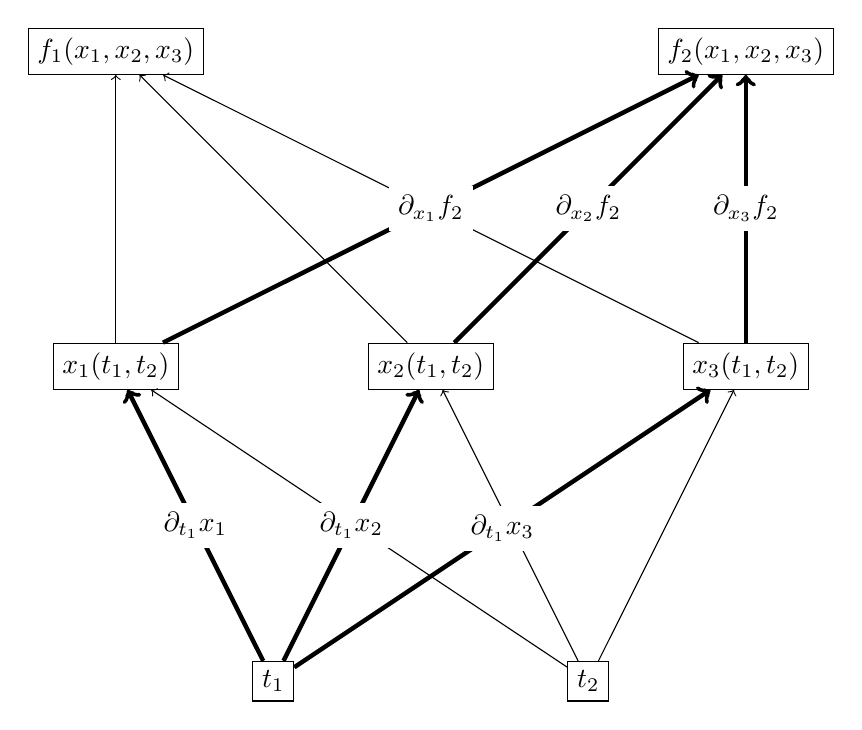
\begin{tikzpicture}[scale=2]
        

\path
    (-2, 0) node[draw](f1) {\(f_1(x_1, x_2, x_3)\)}
    ( 2, 0) node[draw](f2) {\(f_2(x_1, x_2, x_3)\)}
    (-2,-2) node[draw](x1){\(x_1(t_1, t_2)\)}
    ( 0,-2) node[draw](x2){\(x_2(t_1, t_2)\)}
    ( 2,-2) node[draw](x3){\(x_3(t_1, t_2)\)}
    (-1,-4) node[draw](t1){\(t_1\)}
    ( 1,-4) node[draw](t2){\(t_2\)}
;

\path[draw, <-] 
    (f1) edge (x1)
         edge (x2)
         edge (x3)

    (f2) edge (x1)
         edge (x2)
         edge (x3)

    (x1) edge (t1)
         edge (t2)

    (x2) edge (t1)
         edge (t2)

    (x3) edge (t1)
         --   (t2);





\path[draw, ultra thick, <-]
    (f2) edge node[fill=white]{\(\partial_{x_1} f_2\)} (x1)
         edge node[fill=white]{\(\partial_{x_2} f_2\)} (x2)
         edge node[fill=white]{\(\partial_{x_3} f_2\)} (x3)

    (x1) edge node[fill=white]{\(\partial_{t_1} x_1\)} (t1)
    (x2) edge node[fill=white]{\(\partial_{t_1} x_2\)} (t1)
    (x3) --   node[fill=white]{\(\partial_{t_1} x_3\)} (t1)
;

    \end{tikzpicture}
\end{center}
\[
    \partial_{t_1} f_2 = \partial_{x_1} f_2 \cdot \partial_{t_1} x_1 +
                         \partial_{x_2} f_2 \cdot \partial_{t_1} x_2 +
                         \partial_{x_3} f_2 \cdot \partial_{t_1} x_3
\]


Why does it work? Turns out, this is just another way to do, or \emph{visualize}, derivative matrix multiplication. Tracing the ``paths'' of each component is the same thing as component-wise matrix multiplication:
\begin{align*}
    D_{\vec t}\vec f &= D_{\vec x}\vec f \, D_{\vec t} \vec x \\
    &=
    \left(\begin{array}{ccc}
        \partial_{x_1} f_1 & \partial_{x_2} f_1 & \partial_{x_3} f_1 \\ \hline
        \multicolumn{1}{|c}{\partial_{x_1} f_2} & \partial_{x_2} f_2 & \multicolumn{1}{c|}{\partial_{x_3} f_2} \\ \hline
    \end{array}\right)
    \left(\begin{array}{|c|c}
        \cline{1-1}
        \partial_{t_1} x_1 & \partial_{t_2} x_1 \\
        \partial_{t_1} x_2 & \partial_{t_2} x_2 \\
        \partial_{t_1} x_3 & \partial_{t_2} x_3 \\
        \cline{1-1}
    \end{array}\right) \\
    &=
    \left(\begin{array}{cc}
        \partial_{x_1} f_1 \, \partial_{t_1} x_1 + \partial_{x_2} f_1 \, \partial_{t_1} x_2 + \partial_{x_3} f_1 \, \partial_{t_1} x_3 &
        \partial_{x_1} f_1 \, \partial_{t_2} x_1 + \partial_{x_2} f_1 \, \partial_{t_2} x_2 + \partial_{x_3} f_1 \, \partial_{t_2} x_3 \\
        \cline{1-1}
        \multicolumn{1}{|c|}{\partial_{x_1} f_2 \, \partial_{t_1} x_1 + \partial_{x_2} f_2 \, \partial_{t_1} x_2 + \partial_{x_3} f_2 \, \partial_{t_1} x_3} &
        \partial_{x_1} f_2 \, \partial_{t_2} x_1 + \partial_{x_2} f_2 \, \partial_{t_2} x_2 + \partial_{x_3} f_2 \, \partial_{t_2} x_3 \\
        \cline{1-1}
    \end{array}\right)
\end{align*}


\section*{Implicit Derivatives}

Consider some surface defined by the equation \(F(x, y, z) = 0\). Implicitly take partial derivatives with respect to each variable, considering that \(z\) to be a function of \(x\) and \(y\):
\begin{align*}
    \partial_x F + \partial_z F \, \partial_x z &= 0, \\
    \partial_y F + \partial_z F \, \partial_y z &= 0.
\end{align*}
Consequently,
\begin{align*}
    \partial_x z &= -\frac{\partial_x F}{\partial_z F}, \\
    \partial_y z &= -\frac{\partial_y F}{\partial_z F}. \\
\end{align*}

\paragraph{Example}

Consider the surface given by 
\[
    x^2 + y^2 + z^2 - 1 = 0,
\]
a sphere with radius \(1\). The partial derivatives of \(z\) with respect to \(x\) and \(y\) are then
\begin{align*}
    \partial_x z &= - \frac{\partial_x (x^2 + y^2 + z^2 - 1)}{\partial_z (x^2 + y^2 + z^2 - 1)} = - \frac{2x}{2z} = - \frac x z \\
    \partial_y z &= - \frac y z.
\end{align*}





\section*{Directional Derivatives}

%Visualization: cut a plane along some direction, and take a derivative in the cross-section.

Consider the derivative of a function \(\vec f\) along some direction \(\uvec v\). The \emph{directional derivative} can be thought of as a derivative of a function inside a ``cross section'':
\begin{center}
    \begin{tikzpicture}[tdplot_main_coords]
        \path[draw,thick,->] (0,0,0) -- (6,0,0) node[below left]{\(x\)};
\path[draw,thick,->] (0,0,0) -- (0,6,0) node[below right]{\(y\)};
\path[draw,thick,->] (0,0,0) -- (0,0,3) node[above]{\(z\)};
\path[fill=gray,opacity=0.5] (0.0,0.0,0.0) -- (0.05000000000000002,0.08660254037844387,0.08645827496274945) -- (0.10000000000000003,0.17320508075688773,0.17205268742137708) -- (0.15000000000000002,0.25980762113533157,0.25592800630034734) -- (0.20000000000000007,0.34641016151377546,0.3372461771389158) -- (0.25000000000000006,0.4330127018922193,0.41519469565427686) -- (0.30000000000000004,0.5196152422706631,0.48899472601577965) -- (0.3500000000000001,0.6062177826491071,0.5579088827150986) -- (0.40000000000000013,0.6928203230275509,0.6212485982784857) -- (0.45000000000000007,0.7794228634059946,0.6783810032053577) -- (0.5000000000000001,0.8660254037844386,0.7287352493911478) -- (0.5500000000000002,0.9526279441628825,0.7718082138528681) -- (0.6000000000000001,1.0392304845413263,0.8071695257676462) -- (0.6500000000000001,1.12583302491977,0.8344658665957255) -- (0.7000000000000002,1.2124355652982142,0.8534245003225223) -- (0.7500000000000002,1.299038105676658,0.8638559985467295) -- (0.8000000000000003,1.3856406460551018,0.8656561331862856) -- (0.8500000000000003,1.4722431864335457,0.8588069178909179) -- (0.9000000000000001,1.5588457268119893,0.8433767877558079) -- (0.9500000000000002,1.6454482671904334,0.8195199155407428) -- (1.0000000000000002,1.7320508075688772,0.787474671226862) -- (1.0500000000000003,1.818653347947321,0.7475612403026004) -- (1.1000000000000003,1.905255888325765,0.700178424576127) -- (1.1500000000000004,1.991858428704209,0.6457996574795044) -- (1.2000000000000002,2.0784609690826525,0.5849682736783317) -- (1.2500000000000002,2.1650635094610964,0.5182920802513677) -- (1.3000000000000003,2.25166604983954,0.4464372836831155) -- (1.3500000000000003,2.3382685902179845,0.37012183334884746) -- (1.4000000000000004,2.4248711305964283,0.2901082480017695) -- (1.4500000000000002,2.5114736709748717,0.20719599693769522) -- (1.5000000000000004,2.598076211353316,0.12221351196210974) -- (1.5500000000000005,2.68467875173176,0.036009909973414835) -- (1.6000000000000005,2.7712812921102037,-0.05055349113244078) -- (1.6500000000000006,2.8578838324886475,-0.13661177846566347) -- (1.7000000000000006,2.9444863728670914,-0.2213050860663073) -- (1.7500000000000004,3.031088913245535,-0.3037871864007117) -- (1.8000000000000003,3.1176914536239786,-0.383233945587293) -- (1.8500000000000005,3.204293994002423,-0.4588515578698667) -- (1.9000000000000004,3.2908965343808667,-0.5298844770623632) -- (1.9500000000000006,3.377499074759311,-0.5956229657165737) -- (2.0000000000000004,3.4641016151377544,-0.6554101865841192) -- (2.0500000000000003,3.550704155516198,-0.7086487655171197) -- (2.1000000000000005,3.637306695894642,-0.7548067602332117) -- (2.1500000000000004,3.723909236273086,-0.7934229753069951) -- (2.2000000000000006,3.81051177665153,-0.8241115702822773) -- (2.2500000000000004,3.8971143170299736,-0.8465659148623654) -- (2.3000000000000007,3.983716857408418,-0.8605616526586352) -- (2.35,4.070319397786861,-0.8659589428854017) -- (2.4000000000000004,4.156921938165305,-0.8627038576028263) -- (2.4500000000000006,4.243524478543749,-0.8508289205470642) -- (2.5000000000000004,4.330127018922193,-0.8304527821638443) -- (2.5000000000000004,4.330127018922193,-2) -- (0.0,0.0,-2);
\path[fill=black!50.0] (0.0,0.0,0.0) -- (0.0,0.0,0.0) -- (0.09986295347545739,0.005233595624294383,0.005224877325211978) -- (0.1,0.0,0.0);
\path[fill=black!50.0] (0.1,0.0,0.0) -- (0.09986295347545739,0.005233595624294383,0.005224877325211978) -- (0.19972590695091477,0.010467191248588767,0.010397549403305256) -- (0.2,0.0,0.0);
\path[fill=black!50.0] (0.2,0.0,0.0) -- (0.19972590695091477,0.010467191248588767,0.010397549403305256) -- (0.2995888604263721,0.01570078687288315,0.015466332604733584) -- (0.3,0.0,0.0);
\path[fill=black!50.0] (0.3,0.0,0.0) -- (0.2995888604263721,0.01570078687288315,0.015466332604733584) -- (0.39945181390182954,0.020934382497177533,0.020380581323265253) -- (0.4,0.0,0.0);
\path[fill=black!50.0] (0.4,0.0,0.0) -- (0.39945181390182954,0.020934382497177533,0.020380581323265253) -- (0.4993147673772869,0.026167978121471914,0.025091194010139345) -- (0.5,0.0,0.0);
\path[fill=black!50.0] (0.5,0.0,0.0) -- (0.4993147673772869,0.026167978121471914,0.025091194010139345) -- (0.5991777208527442,0.0314015737457663,0.029551103780510145) -- (0.6,0.0,0.0);
\path[fill=black!50.0] (0.6,0.0,0.0) -- (0.5991777208527442,0.0314015737457663,0.029551103780510145) -- (0.6990406743282017,0.036635169370060686,0.033715748690202274) -- (0.7000000000000001,0.0,0.0);
\path[fill=black!50.0] (0.7000000000000001,0.0,0.0) -- (0.6990406743282017,0.036635169370060686,0.033715748690202274) -- (0.7989036278036591,0.041868764994355066,0.03754351698392666) -- (0.8,0.0,0.0);
\path[fill=black!50.0] (0.8,0.0,0.0) -- (0.7989036278036591,0.041868764994355066,0.03754351698392666) -- (0.8987665812791163,0.04710236061864944,0.04099616286618438) -- (0.8999999999999999,0.0,0.0);
\path[fill=black!50.0] (0.8999999999999999,0.0,0.0) -- (0.8987665812791163,0.04710236061864944,0.04099616286618438) -- (0.9986295347545738,0.05233595624294383,0.044039188640612924) -- (1.0,0.0,0.0);
\path[fill=black!50.0] (1.0,0.0,0.0) -- (0.9986295347545738,0.05233595624294383,0.044039188640612924) -- (1.0984924882300313,0.057569551867238215,0.04664218939956477) -- (1.1,0.0,0.0);
\path[fill=black!50.0] (1.1,0.0,0.0) -- (1.0984924882300313,0.057569551867238215,0.04664218939956477) -- (1.1983554417054885,0.0628031474915326,0.048779156819894115) -- (1.2,0.0,0.0);
\path[fill=black!50.0] (1.2,0.0,0.0) -- (1.1983554417054885,0.0628031474915326,0.048779156819894115) -- (1.298218395180946,0.06803674311582698,0.050428739029524564) -- (1.3,0.0,0.0);
\path[fill=black!50.0] (1.3,0.0,0.0) -- (1.298218395180946,0.06803674311582698,0.050428739029524564) -- (1.3980813486564034,0.07327033874012137,0.051574453948296864) -- (1.4000000000000001,0.0,0.0);
\path[fill=black!50.0] (1.4000000000000001,0.0,0.0) -- (1.3980813486564034,0.07327033874012137,0.051574453948296864) -- (1.4979443021318608,0.07850393436441575,0.05220485397146563) -- (1.5,0.0,0.0);
\path[fill=black!50.0] (1.5,0.0,0.0) -- (1.4979443021318608,0.07850393436441575,0.05220485397146563) -- (1.5978072556073182,0.08373752998871013,0.05231364035038191) -- (1.6,0.0,0.0);
\path[fill=black!50.0] (1.6,0.0,0.0) -- (1.5978072556073182,0.08373752998871013,0.05231364035038191) -- (1.6976702090827758,0.08897112561300452,0.05189972612750758) -- (1.7000000000000002,0.0,0.0);
\path[fill=black!50.0] (1.7000000000000002,0.0,0.0) -- (1.6976702090827758,0.08897112561300452,0.05189972612750758) -- (1.7975331625582327,0.09420472123729888,0.050967246996935736) -- (1.7999999999999998,0.0,0.0);
\path[fill=black!50.0] (1.7999999999999998,0.0,0.0) -- (1.7975331625582327,0.09420472123729888,0.050967246996935736) -- (1.8973961160336903,0.09943831686159327,0.04952551998190243) -- (1.9,0.0,0.0);
\path[fill=black!50.0] (1.9,0.0,0.0) -- (1.8973961160336903,0.09943831686159327,0.04952551998190243) -- (1.9972590695091477,0.10467191248588766,0.0475889503421703) -- (2.0,0.0,0.0);
\path[fill=black!50.0] (2.0,0.0,0.0) -- (1.9972590695091477,0.10467191248588766,0.0475889503421703) -- (2.097122022984605,0.10990550811018204,0.04517688764143471) -- (2.1,0.0,0.0);
\path[fill=black!50.0] (2.1,0.0,0.0) -- (2.097122022984605,0.10990550811018204,0.04517688764143471) -- (2.1969849764600626,0.11513910373447643,0.04231343241287951) -- (2.2,0.0,0.0);
\path[fill=black!50.0] (2.2,0.0,0.0) -- (2.1969849764600626,0.11513910373447643,0.04231343241287951) -- (2.2968479299355202,0.12037269935877082,0.03902719535461596) -- (2.3000000000000003,0.0,0.0);
\path[fill=black!50.0] (2.3000000000000003,0.0,0.0) -- (2.2968479299355202,0.12037269935877082,0.03902719535461596) -- (2.396710883410977,0.1256062949830652,0.035351011461044704) -- (2.4,0.0,0.0);
\path[fill=black!50.0] (2.4,0.0,0.0) -- (2.396710883410977,0.1256062949830652,0.035351011461044704) -- (2.4965738368864345,0.13083989060735957,0.03132161194644544) -- (2.5,0.0,0.0);
\path[fill=black!50.0] (2.5,0.0,0.0) -- (2.4965738368864345,0.13083989060735957,0.03132161194644544) -- (2.596436790361892,0.13607348623165397,0.026979257238825664) -- (2.6,0.0,0.0);
\path[fill=black!50.0] (2.6,0.0,0.0) -- (2.596436790361892,0.13607348623165397,0.026979257238825664) -- (2.6962997438373497,0.14130708185594834,0.022367334711032288) -- (2.7,0.0,0.0);
\path[fill=black!50.0] (2.7,0.0,0.0) -- (2.6962997438373497,0.14130708185594834,0.022367334711032288) -- (2.796162697312807,0.14654067748024274,0.01753192516846412) -- (2.8000000000000003,0.0,0.0);
\path[fill=black!50.0] (2.8000000000000003,0.0,0.0) -- (2.796162697312807,0.14654067748024274,0.01753192516846412) -- (2.896025650788264,0.1517742731045371,0.012521342424896647) -- (2.9,0.0,0.0);
\path[fill=black!50.0] (2.9,0.0,0.0) -- (2.896025650788264,0.1517742731045371,0.012521342424896647) -- (2.9958886042637216,0.1570078687288315,0.007385650566825091) -- (3.0,0.0,0.0);
\path[fill=black!50.0] (3.0,0.0,0.0) -- (2.9958886042637216,0.1570078687288315,0.007385650566825091) -- (3.0957515577391788,0.16224146435312586,0.0021761637296613093) -- (3.1,0.0,0.0);
\path[fill=black!50.0] (3.1,0.0,0.0) -- (3.0957515577391788,0.16224146435312586,0.0021761637296613093) -- (3.1956145112146364,0.16747505997742027,-0.0030550666161451583) -- (3.2,0.0,-0.0);
\path[fill=black!50.0] (3.2,0.0,-0.0) -- (3.1956145112146364,0.16747505997742027,-0.0030550666161451583) -- (3.295477464690094,0.17270865560171464,-0.008255771746193862) -- (3.3000000000000003,0.0,-0.0);
\path[fill=black!50.0] (3.3000000000000003,0.0,-0.0) -- (3.295477464690094,0.17270865560171464,-0.008255771746193862) -- (3.3953404181655515,0.17794225122600904,-0.013373987933949906) -- (3.4000000000000004,0.0,-0.0);
\path[fill=black!50.0] (3.4000000000000004,0.0,-0.0) -- (3.3953404181655515,0.17794225122600904,-0.013373987933949906) -- (3.4952033716410082,0.1831758468503034,-0.018358575655122545) -- (3.5,0.0,-0.0);
\path[fill=black!50.0] (3.5,0.0,-0.0) -- (3.4952033716410082,0.1831758468503034,-0.018358575655122545) -- (3.5950663251164654,0.18840944247459776,-0.023159730556887484) -- (3.5999999999999996,0.0,-0.0);
\path[fill=black!50.0] (3.5999999999999996,0.0,-0.0) -- (3.5950663251164654,0.18840944247459776,-0.023159730556887484) -- (3.6949292785919234,0.19364303809889216,-0.02772948108651713) -- (3.7,0.0,-0.0);
\path[fill=black!50.0] (3.7,0.0,-0.0) -- (3.6949292785919234,0.19364303809889216,-0.02772948108651713) -- (3.7947922320673806,0.19887663372318654,-0.03202216780727803) -- (3.8,0.0,-0.0);
\path[fill=black!50.0] (3.8,0.0,-0.0) -- (3.7947922320673806,0.19887663372318654,-0.03202216780727803) -- (3.894655185542838,0.20411022934748094,-0.035994899612430006) -- (3.9000000000000004,0.0,-0.0);
\path[fill=black!50.0] (3.9000000000000004,0.0,-0.0) -- (3.894655185542838,0.20411022934748094,-0.035994899612430006) -- (3.9945181390182953,0.2093438249717753,-0.03960798227898643) -- (4.0,0.0,-0.0);
\path[fill=black!50.0] (4.0,0.0,-0.0) -- (3.9945181390182953,0.2093438249717753,-0.03960798227898643) -- (4.0943810924937525,0.21457742059606968,-0.04282531507926946) -- (4.1,0.0,-0.0);
\path[fill=black!50.0] (4.1,0.0,-0.0) -- (4.0943810924937525,0.21457742059606968,-0.04282531507926946) -- (4.19424404596921,0.21981101622036409,-0.04561475148744752) -- (4.2,0.0,-0.0);
\path[fill=black!50.0] (4.2,0.0,-0.0) -- (4.19424404596921,0.21981101622036409,-0.04561475148744752) -- (4.294106999444668,0.22504461184465846,-0.047948420376995114) -- (4.3,0.0,-0.0);
\path[fill=black!50.0] (4.3,0.0,-0.0) -- (4.294106999444668,0.22504461184465846,-0.047948420376995114) -- (4.393969952920125,0.23027820746895286,-0.04980300449977631) -- (4.4,0.0,-0.0);
\path[fill=black!50.0] (4.4,0.0,-0.0) -- (4.393969952920125,0.23027820746895286,-0.04980300449977631) -- (4.493832906395582,0.23551180309324724,-0.05115997346428025) -- (4.5,0.0,-0.0);
\path[fill=black!50.0] (4.5,0.0,-0.0) -- (4.493832906395582,0.23551180309324724,-0.05115997346428025) -- (4.5936958598710405,0.24074539871754164,-0.05200576888516793) -- (4.6000000000000005,0.0,-0.0);
\path[fill=black!50.0] (4.6000000000000005,0.0,-0.0) -- (4.5936958598710405,0.24074539871754164,-0.05200576888516793) -- (4.693558813346496,0.24597899434183595,-0.05233193985417663) -- (4.699999999999999,0.0,-0.0);
\path[fill=black!50.0] (4.699999999999999,0.0,-0.0) -- (4.693558813346496,0.24597899434183595,-0.05233193985417663) -- (4.793421766821954,0.2512125899661304,-0.052135227378801816) -- (4.8,0.0,-0.0);
\path[fill=black!50.0] (4.8,0.0,-0.0) -- (4.793421766821954,0.2512125899661304,-0.052135227378801816) -- (4.893284720297412,0.25644618559042476,-0.051417596945072905) -- (4.9,0.0,-0.0);
\path[fill=black!50.0] (4.9,0.0,-0.0) -- (4.893284720297412,0.25644618559042476,-0.051417596945072905) -- (4.993147673772869,0.26167978121471913,-0.050186218879066664) -- (5.0,0.0,-0.0);
\path[fill=black!50.0] (0.0,0.0,0.0) -- (0.0,0.0,0.0) -- (0.09945218953682733,0.010452846326765346,0.01043543362485232) -- (0.09986295347545739,0.005233595624294383,0.005224877325211978);
\path[fill=black!49.7387561337394] (0.09986295347545739,0.005233595624294383,0.005224877325211978) -- (0.09945218953682733,0.010452846326765346,0.01043543362485232) -- (0.19890437907365466,0.02090569265353069,0.02076659984642085) -- (0.19972590695091477,0.010467191248588767,0.010397549403305256);
\path[fill=black!49.48012252983474] (0.19972590695091477,0.010467191248588767,0.010397549403305256) -- (0.19890437907365466,0.02090569265353069,0.02076659984642085) -- (0.298356568610482,0.03135853898029604,0.03089027306684919) -- (0.2995888604263721,0.01570078687288315,0.015466332604733584);
\path[fill=black!49.22668336976332] (0.2995888604263721,0.01570078687288315,0.015466332604733584) -- (0.298356568610482,0.03135853898029604,0.03089027306684919) -- (0.3978087581473093,0.04181138530706138,0.04070530088976028) -- (0.39945181390182954,0.020934382497177533,0.020380581323265253);
\path[fill=black!48.980970933836744] (0.39945181390182954,0.020934382497177533,0.020380581323265253) -- (0.3978087581473093,0.04181138530706138,0.04070530088976028) -- (0.49726094768413664,0.05226423163382673,0.050113614801564406) -- (0.4993147673772869,0.026167978121471914,0.025091194010139345);
\path[fill=black!48.74544029949304] (0.4993147673772869,0.026167978121471914,0.025091194010139345) -- (0.49726094768413664,0.05226423163382673,0.050113614801564406) -- (0.596713137220964,0.06271707796059207,0.05902121003962995) -- (0.5991777208527442,0.0314015737457663,0.029551103780510145);
\path[fill=black!48.5224448109745] (0.5991777208527442,0.0314015737457663,0.029551103780510145) -- (0.596713137220964,0.06271707796059207,0.05902121003962995) -- (0.6961653267577914,0.07316992428735743,0.06733908485679765) -- (0.6990406743282017,0.036635169370060686,0.033715748690202274);
\path[fill=black!48.31421256548989] (0.6990406743282017,0.036635169370060686,0.033715748690202274) -- (0.6961653267577914,0.07316992428735743,0.06733908485679765) -- (0.7956175162946186,0.08362277061412277,0.07498412979741824) -- (0.7989036278036591,0.041868764994355066,0.03754351698392666);
\path[fill=black!48.122824150803666] (0.7989036278036591,0.041868764994355066,0.03754351698392666) -- (0.7956175162946186,0.08362277061412277,0.07498412979741824) -- (0.8950697058314458,0.0940756169408881,0.08187995809956089) -- (0.8987665812791163,0.04710236061864944,0.04099616286618438);
\path[fill=black!47.95019185669078] (0.8987665812791163,0.04710236061864944,0.04099616286618438) -- (0.8950697058314458,0.0940756169408881,0.08187995809956089) -- (0.9945218953682733,0.10452846326765346,0.0879576689262884) -- (0.9986295347545738,0.05233595624294383,0.044039188640612924);
\path[fill=black!47.79804056796936] (0.9986295347545738,0.05233595624294383,0.044039188640612924) -- (0.9945218953682733,0.10452846326765346,0.0879576689262884) -- (1.0939740849051007,0.11498130959441881,0.09315653580004415) -- (1.0984924882300313,0.057569551867238215,0.04664218939956477);
\path[fill=black!47.667890530021765] (1.0984924882300313,0.057569551867238215,0.04664218939956477) -- (1.0939740849051007,0.11498130959441881,0.09315653580004415) -- (1.193426274441928,0.12543415592118415,0.09742461336154251) -- (1.1983554417054885,0.0628031474915326,0.048779156819894115);
\path[fill=black!47.5610421590053] (1.1983554417054885,0.0628031474915326,0.048779156819894115) -- (1.193426274441928,0.12543415592118415,0.09742461336154251) -- (1.2928784639787554,0.1358870022479495,0.10071925639062787) -- (1.298218395180946,0.06803674311582698,0.050428739029524564);
\path[fill=black!47.47856304852377] (1.298218395180946,0.06803674311582698,0.050428739029524564) -- (1.2928784639787554,0.1358870022479495,0.10071925639062787) -- (1.3923306535155828,0.14633984857471485,0.10300754590321778) -- (1.3980813486564034,0.07327033874012137,0.051574453948296864);
\path[fill=black!47.42127730258515] (1.3980813486564034,0.07327033874012137,0.051574453948296864) -- (1.3923306535155828,0.14633984857471485,0.10300754590321778) -- (1.4917828430524098,0.15679269490148018,0.10426661806691039) -- (1.4979443021318608,0.07850393436441575,0.05220485397146563);
\path[fill=black!47.38975730142671] (1.4979443021318608,0.07850393436441575,0.05220485397146563) -- (1.4917828430524098,0.15679269490148018,0.10426661806691039) -- (1.5912350325892373,0.16724554122824553,0.10448389264883999) -- (1.5978072556073182,0.08373752998871013,0.05231364035038191);
\path[fill=black!47.38431798248091] (1.5978072556073182,0.08373752998871013,0.05231364035038191) -- (1.5912350325892373,0.16724554122824553,0.10448389264883999) -- (1.6906872221260647,0.17769838755501088,0.10365719871320539) -- (1.6976702090827758,0.08897112561300452,0.05189972612750758);
\path[fill=black!47.40501369362462] (1.6976702090827758,0.08897112561300452,0.05189972612750758) -- (1.6906872221260647,0.17769838755501088,0.10365719871320539) -- (1.7901394116628917,0.1881512338817762,0.10179479631254278) -- (1.7975331625582327,0.09420472123729888,0.050967246996935736);
\path[fill=black!47.45163765015321] (1.7975331625582327,0.09420472123729888,0.050967246996935736) -- (1.7901394116628917,0.1881512338817762,0.10179479631254278) -- (1.8895916011997191,0.19860408020854156,0.09891529395601115) -- (1.8973961160336903,0.09943831686159327,0.04952551998190243);
\path[fill=black!47.52372400090488] (1.8973961160336903,0.09943831686159327,0.04952551998190243) -- (1.8895916011997191,0.19860408020854156,0.09891529395601115) -- (1.9890437907365466,0.20905692653530691,0.09504746267932007) -- (1.9972590695091477,0.10467191248588766,0.0475889503421703);
\path[fill=black!47.62055248289149] (1.9972590695091477,0.10467191248588766,0.0475889503421703) -- (1.9890437907365466,0.20905692653530691,0.09504746267932007) -- (2.088495980273374,0.21950977286207227,0.0902299485740512) -- (2.097122022984605,0.10990550811018204,0.04517688764143471);
\path[fill=black!47.741155617928264] (2.097122022984605,0.10990550811018204,0.04517688764143471) -- (2.088495980273374,0.21950977286207227,0.0902299485740512) -- (2.1879481698102015,0.22996261918883762,0.08451088664868595) -- (2.1969849764600626,0.11513910373447643,0.04231343241287951);
\path[fill=black!47.88432837935602] (2.1969849764600626,0.11513910373447643,0.04231343241287951) -- (2.1879481698102015,0.22996261918883762,0.08451088664868595) -- (2.287400359347029,0.24041546551560297,0.07794741987951201) -- (2.2968479299355202,0.12037269935877082,0.03902719535461596);
\path[fill=black!48.0486402322692] (2.2968479299355202,0.12037269935877082,0.03902719535461596) -- (2.287400359347029,0.24041546551560297,0.07794741987951201) -- (2.386852548883856,0.2508683118423683,0.07060512825689336) -- (2.396710883410977,0.1256062949830652,0.035351011461044704);
\path[fill=black!48.23244942694777] (2.396710883410977,0.1256062949830652,0.035351011461044704) -- (2.386852548883856,0.2508683118423683,0.07060512825689336) -- (2.4863047384206833,0.26132115816913365,0.06255737353168422) -- (2.4965738368864345,0.13083989060735957,0.03132161194644544);
\path[fill=black!48.43391940267773] (2.4965738368864345,0.13083989060735957,0.03132161194644544) -- (2.4863047384206833,0.26132115816913365,0.06255737353168422) -- (2.5857569279575108,0.271774004495899,0.053884566208864886) -- (2.596436790361892,0.13607348623165397,0.026979257238825664);
\path[fill=black!48.65103713805872] (2.596436790361892,0.13607348623165397,0.026979257238825664) -- (2.5857569279575108,0.271774004495899,0.053884566208864886) -- (2.685209117494338,0.28222685082266435,0.04467336211235601) -- (2.6962997438373497,0.14130708185594834,0.022367334711032288);
\path[fill=black!48.88163326444839] (2.6962997438373497,0.14130708185594834,0.022367334711032288) -- (2.685209117494338,0.28222685082266435,0.04467336211235601) -- (2.7846613070311657,0.2926796971494297,0.03501579654867066) -- (2.796162697312807,0.14654067748024274,0.01753192516846412);
\path[fill=black!49.1234037415768] (2.796162697312807,0.14654067748024274,0.01753192516846412) -- (2.7846613070311657,0.2926796971494297,0.03501579654867066) -- (2.8841134965679927,0.303132543476195,0.025008364720554493) -- (2.896025650788264,0.1517742731045371,0.012521342424896647);
\path[fill=black!49.37393287875517] (2.896025650788264,0.1517742731045371,0.012521342424896647) -- (2.8841134965679927,0.303132543476195,0.025008364720554493) -- (2.9835656861048196,0.31358538980296036,0.01475105757881679) -- (2.9958886042637216,0.1570078687288315,0.007385650566825091);
\path[fill=black!49.63071747165875] (2.9958886042637216,0.1570078687288315,0.007385650566825091) -- (2.9835656861048196,0.31358538980296036,0.01475105757881679) -- (3.083017875641647,0.3240382361297257,0.004346362745802903) -- (3.0957515577391788,0.16224146435312586,0.0021761637296613093);
\path[fill=black!49.89119181351693] (3.0957515577391788,0.16224146435312586,0.0021761637296613093) -- (3.083017875641647,0.3240382361297257,0.004346362745802903) -- (3.1824700651784745,0.33449108245649106,-0.00610175950705054) -- (3.1956145112146364,0.16747505997742027,-0.0030550666161451583);
\path[fill=black!50.152753330807265] (3.1956145112146364,0.16747505997742027,-0.0030550666161451583) -- (3.1824700651784745,0.33449108245649106,-0.00610175950705054) -- (3.281922254715302,0.3449439287832564,-0.016488914995883064) -- (3.295477464690094,0.17270865560171464,-0.008255771746193862);
\path[fill=black!50.412788587309684] (3.295477464690094,0.17270865560171464,-0.008255771746193862) -- (3.281922254715302,0.3449439287832564,-0.016488914995883064) -- (3.3813744442521294,0.35539677511002177,-0.02671131869658736) -- (3.3953404181655515,0.17794225122600904,-0.013373987933949906);
\path[fill=black!50.66869939669749] (3.3953404181655515,0.17794225122600904,-0.013373987933949906) -- (3.3813744442521294,0.35539677511002177,-0.02671131869658736) -- (3.4808266337889564,0.3658496214367871,-0.036666831730463346) -- (3.4952033716410082,0.1831758468503034,-0.018358575655122545);
\path[fill=black!50.91792878275613] (3.4952033716410082,0.1831758468503034,-0.018358575655122545) -- (3.4808266337889564,0.3658496214367871,-0.036666831730463346) -- (3.5802788233257834,0.3763024677635524,-0.04625598190213167) -- (3.5950663251164654,0.18840944247459776,-0.023159730556887484);
\path[fill=black!51.15798652784438] (3.5950663251164654,0.18840944247459776,-0.023159730556887484) -- (3.5802788233257834,0.3763024677635524,-0.04625598190213167) -- (3.6797310128626113,0.3867553140903178,-0.05538295759282871) -- (3.6949292785919234,0.19364303809889216,-0.02772948108651713);
\path[fill=black!51.38647405432586] (3.6949292785919234,0.19364303809889216,-0.02772948108651713) -- (3.6797310128626113,0.3867553140903178,-0.05538295759282871) -- (3.7791832023994383,0.3972081604170831,-0.06395656507842991) -- (3.7947922320673806,0.19887663372318654,-0.03202216780727803);
\path[fill=black!51.601108390363905] (3.7947922320673806,0.19887663372318654,-0.03202216780727803) -- (3.7791832023994383,0.3972081604170831,-0.06395656507842991) -- (3.878635391936266,0.40766100674384853,-0.07189113970699713) -- (3.894655185542838,0.20411022934748094,-0.035994899612430006);
\path[fill=black!51.7997449806215] (3.894655185542838,0.20411022934748094,-0.035994899612430006) -- (3.878635391936266,0.40766100674384853,-0.07189113970699713) -- (3.978087581473093,0.41811385307061383,-0.07910740183166325) -- (3.9945181390182953,0.2093438249717753,-0.03960798227898643);
\path[fill=black!51.98039911394932] (3.9945181390182953,0.2093438249717753,-0.03960798227898643) -- (3.978087581473093,0.41811385307061383,-0.07910740183166325) -- (4.07753977100992,0.4285666993973791,-0.0855332489466578) -- (4.0943810924937525,0.21457742059606968,-0.04282531507926946);
\path[fill=black!52.141265753963474] (4.0943810924937525,0.21457742059606968,-0.04282531507926946) -- (4.07753977100992,0.4285666993973791,-0.0855332489466578) -- (4.176991960546748,0.43901954572414453,-0.09110447611171044) -- (4.19424404596921,0.21981101622036409,-0.04561475148744752);
\path[fill=black!52.280737574372374] (4.19424404596921,0.21981101622036409,-0.04561475148744752) -- (4.176991960546748,0.43901954572414453,-0.09110447611171044) -- (4.276444150083575,0.44947239205090983,-0.09576541746659072) -- (4.294106999444668,0.22504461184465846,-0.047948420376995114);
\path[fill=black!52.397421018849755] (4.294106999444668,0.22504461184465846,-0.047948420376995114) -- (4.276444150083575,0.44947239205090983,-0.09576541746659072) -- (4.375896339620403,0.45992523837767524,-0.09946950242598313) -- (4.393969952920125,0.23027820746895286,-0.04980300449977631);
\path[fill=black!52.49015022498882] (4.393969952920125,0.23027820746895286,-0.04980300449977631) -- (4.375896339620403,0.45992523837767524,-0.09946950242598313) -- (4.4753485291572295,0.47037808470444054,-0.10217972099738105) -- (4.493832906395582,0.23551180309324724,-0.05115997346428025);
\path[fill=black!52.557998673214016] (4.493832906395582,0.23551180309324724,-0.05115997346428025) -- (4.4753485291572295,0.47037808470444054,-0.10217972099738105) -- (4.574800718694058,0.48083093103120594,-0.1038689935726983) -- (4.5936958598710405,0.24074539871754164,-0.05200576888516793);
\path[fill=black!52.60028844425839] (4.5936958598710405,0.24074539871754164,-0.05200576888516793) -- (4.574800718694058,0.48083093103120594,-0.1038689935726983) -- (4.6742529082308835,0.4912837773579712,-0.1045204414987615) -- (4.693558813346496,0.24597899434183595,-0.05233193985417663);
\path[fill=black!52.61659699270883] (4.693558813346496,0.24597899434183595,-0.05233193985417663) -- (4.6742529082308835,0.4912837773579712,-0.1045204414987615) -- (4.773705097767712,0.5017366236847366,-0.10412755572323355) -- (4.793421766821954,0.2512125899661304,-0.052135227378801816);
\path[fill=black!52.60676136894009] (4.793421766821954,0.2512125899661304,-0.052135227378801816) -- (4.773705097767712,0.5017366236847366,-0.10412755572323355) -- (4.873157287304539,0.512189470011502,-0.10269426183091271) -- (4.893284720297412,0.25644618559042476,-0.051417596945072905);
\path[fill=black!52.570879847253636] (4.893284720297412,0.25644618559042476,-0.051417596945072905) -- (4.873157287304539,0.512189470011502,-0.10269426183091271) -- (4.972609476841367,0.5226423163382673,-0.1002348808205871) -- (4.993147673772869,0.26167978121471913,-0.050186218879066664);
\path[fill=black!50.0] (0.0,0.0,0.0) -- (0.0,0.0,0.0) -- (0.09876883405951378,0.01564344650402309,0.015617387126285041) -- (0.09945218953682733,0.010452846326765346,0.01043543362485232);
\path[fill=black!49.47822831875739] (0.09945218953682733,0.010452846326765346,0.01043543362485232) -- (0.09876883405951378,0.01564344650402309,0.015617387126285041) -- (0.19753766811902757,0.03128689300804618,0.031078730482826066) -- (0.19890437907365466,0.02090569265353069,0.02076659984642085);
\path[fill=black!48.96167000767896] (0.19890437907365466,0.02090569265353069,0.02076659984642085) -- (0.19753766811902757,0.03128689300804618,0.031078730482826066) -- (0.2963065021785413,0.046930339512069257,0.046229545437645125) -- (0.298356568610482,0.03135853898029604,0.03089027306684919);
\path[fill=black!48.45548634665754] (0.298356568610482,0.03135853898029604,0.03089027306684919) -- (0.2963065021785413,0.046930339512069257,0.046229545437645125) -- (0.39507533623805513,0.06257378601609236,0.06091845005590725) -- (0.3978087581473093,0.04181138530706138,0.04070530088976028);
\path[fill=black!47.964734955511986] (0.3978087581473093,0.04181138530706138,0.04070530088976028) -- (0.39507533623805513,0.06257378601609236,0.06091845005590725) -- (0.4938441702975689,0.07821723252011543,0.07499867765817304) -- (0.49726094768413664,0.05226423163382673,0.050113614801564406);
\path[fill=black!47.49431925992178] (0.49726094768413664,0.05226423163382673,0.050113614801564406) -- (0.4938441702975689,0.07821723252011543,0.07499867765817304) -- (0.5926130043570826,0.09386067902413851,0.08832954326454515) -- (0.596713137220964,0.06271707796059207,0.05902121003962995);
\path[fill=black!47.048939498018505] (0.596713137220964,0.06271707796059207,0.05902121003962995) -- (0.5926130043570826,0.09386067902413851,0.08832954326454515) -- (0.6913818384165965,0.10950412552816162,0.10077784927248298) -- (0.6961653267577914,0.07316992428735743,0.06733908485679765);
\path[fill=black!46.63304575716012] (0.6961653267577914,0.07316992428735743,0.06733908485679765) -- (0.6913818384165965,0.10950412552816162,0.10077784927248298) -- (0.7901506724761103,0.1251475720321847,0.11221921632321807) -- (0.7956175162946186,0.08362277061412277,0.07498412979741824);
\path[fill=black!46.250793510129085] (0.7956175162946186,0.08362277061412277,0.07498412979741824) -- (0.7901506724761103,0.1251475720321847,0.11221921632321807) -- (0.8889195065356239,0.14079101853620776,0.12253932605919263) -- (0.8950697058314458,0.0940756169408881,0.08187995809956089);
\path[fill=black!45.90600209502196] (0.8950697058314458,0.0940756169408881,0.08187995809956089) -- (0.8889195065356239,0.14079101853620776,0.12253932605919263) -- (0.9876883405951378,0.15643446504023087,0.13163506335529954) -- (0.9945218953682733,0.10452846326765346,0.0879576689262884);
\path[fill=black!45.602116553685576] (0.9945218953682733,0.10452846326765346,0.0879576689262884) -- (0.9876883405951378,0.15643446504023087,0.13163506335529954) -- (1.0864571746546516,0.17207791154425398,0.13941554661112707) -- (1.0939740849051007,0.11498130959441881,0.09315653580004415);
\path[fill=black!45.342173209997796] (1.0939740849051007,0.11498130959441881,0.09315653580004415) -- (1.0864571746546516,0.17207791154425398,0.13941554661112707) -- (1.1852260087141653,0.18772135804827703,0.14580303580986878) -- (1.193426274441928,0.12543415592118415,0.09742461336154251);
\path[fill=black!45.12876933192287] (1.193426274441928,0.12543415592118415,0.09742461336154251) -- (1.1852260087141653,0.18772135804827703,0.14580303580986878) -- (1.2839948427736791,0.20336480455230013,0.15073370927087418) -- (1.2928784639787554,0.1358870022479495,0.10071925639062787);
\path[fill=black!44.96403718046861] (1.2928784639787554,0.1358870022479495,0.10071925639062787) -- (1.2839948427736791,0.20336480455230013,0.15073370927087418) -- (1.382763676833193,0.21900825105632324,0.15415830133478473) -- (1.3923306535155828,0.14633984857471485,0.10300754590321778);
\path[fill=black!44.849622704839106] (1.3923306535155828,0.14633984857471485,0.10300754590321778) -- (1.382763676833193,0.21900825105632324,0.15415830133478473) -- (1.4815325108927067,0.23465169756034632,0.1560425946097175) -- (1.4917828430524098,0.15679269490148018,0.10426661806691039);
\path[fill=black!44.786669096654485] (1.4917828430524098,0.15679269490148018,0.10426661806691039) -- (1.4815325108927067,0.23465169756034632,0.1560425946097175) -- (1.5803013449522205,0.2502951440643694,0.15636776186013393) -- (1.5912350325892373,0.16724554122824553,0.10448389264883999);
\path[fill=black!44.775805367558] (1.5912350325892373,0.16724554122824553,0.10448389264883999) -- (1.5803013449522205,0.2502951440643694,0.15636776186013393) -- (1.6790701790117344,0.26593859056839253,0.15513055412235385) -- (1.6906872221260647,0.17769838755501088,0.10365719871320539);
\path[fill=black!44.81714006433973] (1.6906872221260647,0.17769838755501088,0.10365719871320539) -- (1.6790701790117344,0.26593859056839253,0.15513055412235385) -- (1.7778390130712478,0.2815820370724155,0.1523433331671267) -- (1.7901394116628917,0.1881512338817762,0.10179479631254278);
\path[fill=black!44.910260184372866] (1.7901394116628917,0.1881512338817762,0.10179479631254278) -- (1.7778390130712478,0.2815820370724155,0.1523433331671267) -- (1.8766078471307617,0.29722548357643863,0.14803394798490424) -- (1.8895916011997191,0.19860408020854156,0.09891529395601115);
\path[fill=black!45.054235302199444] (1.8895916011997191,0.19860408020854156,0.09891529395601115) -- (1.8766078471307617,0.29722548357643863,0.14803394798490424) -- (1.9753766811902755,0.31286893008046174,0.142245456527934) -- (1.9890437907365466,0.20905692653530691,0.09504746267932007);
\path[fill=black!45.247626866034] (1.9890437907365466,0.20905692653530691,0.09504746267932007) -- (1.9753766811902755,0.31286893008046174,0.142245456527934) -- (2.074145515249789,0.32851237658448484,0.13503569548943306) -- (2.088495980273374,0.21950977286207227,0.0902299485740512);
\path[fill=black!45.48850257129744] (2.088495980273374,0.21950977286207227,0.0902299485740512) -- (2.074145515249789,0.32851237658448484,0.13503569548943306) -- (2.1729143493093033,0.34415582308850795,0.12647670241846803) -- (2.1879481698102015,0.22996261918883762,0.08451088664868595);
\path[fill=black!45.774455667565704] (2.1879481698102015,0.22996261918883762,0.08451088664868595) -- (2.1729143493093033,0.34415582308850795,0.12647670241846803) -- (2.271683183368817,0.35979926959253106,0.11665399594457705) -- (2.287400359347029,0.24041546551560297,0.07794741987951201);
\path[fill=black!46.1026290060244] (2.287400359347029,0.24041546551560297,0.07794741987951201) -- (2.271683183368817,0.35979926959253106,0.11665399594457705) -- (2.3704520174283306,0.37544271609655405,0.10566572130389218) -- (2.386852548883856,0.2508683118423683,0.07060512825689336);
\path[fill=black!46.469743587155335] (2.386852548883856,0.2508683118423683,0.07060512825689336) -- (2.3704520174283306,0.37544271609655405,0.10566572130389218) -- (2.4692208514878446,0.39108616260057716,0.0936216697043824) -- (2.4863047384206833,0.26132115816913365,0.06255737353168422);
\path[fill=black!46.872131323415786] (2.4863047384206833,0.26132115816913365,0.06255737353168422) -- (2.4692208514878446,0.39108616260057716,0.0936216697043824) -- (2.5679896855473583,0.40672960910460026,0.08064218132839589) -- (2.5857569279575108,0.271774004495899,0.053884566208864886);
\path[fill=black!47.30577168955675] (2.5857569279575108,0.271774004495899,0.053884566208864886) -- (2.5679896855473583,0.40672960910460026,0.08064218132839589) -- (2.666758519606872,0.42237305560862337,0.0668569429333371) -- (2.685209117494338,0.28222685082266435,0.04467336211235601);
\path[fill=black!47.7663318943822] (2.685209117494338,0.28222685082266435,0.04467336211235601) -- (2.666758519606872,0.42237305560862337,0.0668569429333371) -- (2.765527353666386,0.4380165021126465,0.05240369206445548) -- (2.7846613070311657,0.2926796971494297,0.03501579654867066);
\path[fill=black!48.24921017256647] (2.7846613070311657,0.2926796971494297,0.03501579654867066) -- (2.765527353666386,0.4380165021126465,0.05240369206445548) -- (2.8642961877258997,0.45365994861666953,0.03742684082682342) -- (2.8841134965679927,0.303132543476195,0.025008364720554493);
\path[fill=black!48.74958176397227] (2.8841134965679927,0.303132543476195,0.025008364720554493) -- (2.8642961877258997,0.45365994861666953,0.03742684082682342) -- (2.9630650217854133,0.46930339512069263,0.022076032967318394) -- (2.9835656861048196,0.31358538980296036,0.01475105757881679);
\path[fill=black!49.26244712105916] (2.9835656861048196,0.31358538980296036,0.01475105757881679) -- (2.9630650217854133,0.46930339512069263,0.022076032967318394) -- (3.061833855844927,0.4849468416247157,0.006504648683770223) -- (3.083017875641647,0.3240382361297257,0.004346362745802903);
\path[fill=black!49.78268186270986] (3.083017875641647,0.3240382361297257,0.004346362745802903) -- (3.061833855844927,0.4849468416247157,0.006504648683770223) -- (3.160602689904441,0.5005902881287388,-0.009131727899275199) -- (3.1824700651784745,0.33449108245649106,-0.00610175950705054);
\path[fill=black!50.30508797535253] (3.1824700651784745,0.33449108245649106,-0.00610175950705054) -- (3.160602689904441,0.5005902881287388,-0.009131727899275199) -- (3.2593715239639547,0.5162337346327619,-0.024676863275698985) -- (3.281922254715302,0.3449439287832564,-0.016488914995883064);
\path[fill=black!50.82444574979416] (3.281922254715302,0.3449439287832564,-0.016488914995883064) -- (3.2593715239639547,0.5162337346327619,-0.024676863275698985) -- (3.3581403580234688,0.5318771811367851,-0.039975435591358466) -- (3.3813744442521294,0.35539677511002177,-0.02671131869658736);
\path[fill=black!51.335565934829376] (3.3813744442521294,0.35539677511002177,-0.02671131869658736) -- (3.3581403580234688,0.5318771811367851,-0.039975435591358466) -- (3.456909192082982,0.547520627640808,-0.05487458656871118) -- (3.4808266337889564,0.3658496214367871,-0.036666831730463346);
\path[fill=black!51.833341586523176] (3.4808266337889564,0.3658496214367871,-0.036666831730463346) -- (3.456909192082982,0.547520627640808,-0.05487458656871118) -- (3.5556780261424956,0.563164074144831,-0.06922544881619601) -- (3.5802788233257834,0.3763024677635524,-0.04625598190213167);
\path[fill=black!52.31279909510658] (3.5802788233257834,0.3763024677635524,-0.04625598190213167) -- (3.5556780261424956,0.563164074144831,-0.06922544881619601) -- (3.6544468602020097,0.5788075206488542,-0.08288463326200055) -- (3.6797310128626113,0.3867553140903178,-0.05538295759282871);
\path[fill=black!52.769147879641444] (3.6797310128626113,0.3867553140903178,-0.05538295759282871) -- (3.6544468602020097,0.5788075206488542,-0.08288463326200055) -- (3.7532156942615233,0.5944509671528773,-0.09571566185026815) -- (3.7791832023994383,0.3972081604170831,-0.06395656507842991);
\path[fill=black!53.1978282539215] (3.7791832023994383,0.3972081604170831,-0.06395656507842991) -- (3.7532156942615233,0.5944509671528773,-0.09571566185026815) -- (3.8519845283210374,0.6100944136569004,-0.10759033118471925) -- (3.878635391936266,0.40766100674384853,-0.07189113970699713);
\path[fill=black!53.594556985349854] (3.878635391936266,0.40766100674384853,-0.07189113970699713) -- (3.8519845283210374,0.6100944136569004,-0.10759033118471925) -- (3.950753362380551,0.6257378601609235,-0.11838999349460758) -- (3.978087581473093,0.41811385307061383,-0.07910740183166325);
\path[fill=black!53.955370091583156] (3.978087581473093,0.41811385307061383,-0.07910740183166325) -- (3.950753362380551,0.6257378601609235,-0.11838999349460758) -- (4.049522196440065,0.6413813066649465,-0.1280067421240266) -- (4.07753977100992,0.4285666993973791,-0.0855332489466578);
\path[fill=black!54.27666244733289] (4.07753977100992,0.4285666993973791,-0.0855332489466578) -- (4.049522196440065,0.6413813066649465,-0.1280067421240266) -- (4.148291030499578,0.6570247531689697,-0.13634448969954568) -- (4.176991960546748,0.43901954572414453,-0.09110447611171044);
\path[fill=black!54.55522380558553] (4.176991960546748,0.43901954572414453,-0.09110447611171044) -- (4.148291030499578,0.6570247531689697,-0.13634448969954568) -- (4.247059864559092,0.6726681996729927,-0.14331992820348297) -- (4.276444150083575,0.44947239205090983,-0.09576541746659072);
\path[fill=black!54.78827087332954] (4.276444150083575,0.44947239205090983,-0.09576541746659072) -- (4.247059864559092,0.6726681996729927,-0.14331992820348297) -- (4.3458286986186065,0.6883116461770159,-0.1488633613600807) -- (4.375896339620403,0.45992523837767524,-0.09946950242598313);
\path[fill=black!54.97347512129915] (4.375896339620403,0.45992523837767524,-0.09946950242598313) -- (4.3458286986186065,0.6883116461770159,-0.1488633613600807) -- (4.44459753267812,0.703955092681039,-0.1529194010176534) -- (4.4753485291572295,0.47037808470444054,-0.10217972099738105);
\path[fill=black!55.108986049869046] (4.4753485291572295,0.47037808470444054,-0.10217972099738105) -- (4.44459753267812,0.703955092681039,-0.1529194010176534) -- (4.543366366737634,0.7195985391850621,-0.15544752056869113) -- (4.574800718694058,0.48083093103120594,-0.1038689935726983);
\path[fill=black!55.193449678634906] (4.574800718694058,0.48083093103120594,-0.1038689935726983) -- (4.543366366737634,0.7195985391850621,-0.15544752056869113) -- (4.642135200797147,0.7352419856890849,-0.1564224598783251) -- (4.6742529082308835,0.4912837773579712,-0.1045204414987615);
\path[fill=black!55.22602207493807] (4.6742529082308835,0.4912837773579712,-0.1045204414987615) -- (4.642135200797147,0.7352419856890849,-0.1564224598783251) -- (4.740904034856661,0.7508854321931081,-0.15583447767524558) -- (4.773705097767712,0.5017366236847366,-0.10412755572323355);
\path[fill=black!55.206377786161674] (4.773705097767712,0.5017366236847366,-0.10412755572323355) -- (4.740904034856661,0.7508854321931081,-0.15583447767524558) -- (4.839672868916176,0.7665288786971313,-0.1536894488832646) -- (4.873157287304539,0.512189470011502,-0.10269426183091271);
\path[fill=black!55.13471309154563] (4.873157287304539,0.512189470011502,-0.10269426183091271) -- (4.839672868916176,0.7665288786971313,-0.1536894488832646) -- (4.938441702975689,0.7821723252011543,-0.15000880592101948) -- (4.972609476841367,0.5226423163382673,-0.1002348808205871);
\path[fill=black!50.0] (0.0,0.0,0.0) -- (0.0,0.0,0.0) -- (0.09781476007338058,0.02079116908177593,0.020756534455155882) -- (0.09876883405951378,0.01564344650402309,0.015617387126285041);
\path[fill=black!49.21913064368575] (0.09876883405951378,0.01564344650402309,0.015617387126285041) -- (0.09781476007338058,0.02079116908177593,0.020756534455155882) -- (0.19562952014676116,0.04158233816355186,0.041305676479233916) -- (0.19753766811902757,0.03128689300804618,0.031078730482826066);
\path[fill=black!48.44606347585869] (0.19753766811902757,0.03128689300804618,0.031078730482826066) -- (0.19562952014676116,0.04158233816355186,0.041305676479233916) -- (0.2934442802201417,0.062373507245327794,0.061442105837772765) -- (0.2963065021785413,0.046930339512069257,0.046229545437645125);
\path[fill=black!47.688522728117746] (0.2963065021785413,0.046930339512069257,0.046229545437645125) -- (0.2934442802201417,0.062373507245327794,0.061442105837772765) -- (0.3912590402935223,0.08316467632710373,0.08096462598484051) -- (0.39507533623805513,0.06257378601609236,0.06091845005590725);
\path[fill=black!46.954077497204636] (0.39507533623805513,0.06257378601609236,0.06091845005590725) -- (0.3912590402935223,0.08316467632710373,0.08096462598484051) -- (0.48907380036690284,0.10395584540887966,0.09967817435241479) -- (0.4938441702975689,0.07821723252011543,0.07499867765817304);
\path[fill=black!46.25006611709135] (0.4938441702975689,0.07821723252011543,0.07499867765817304) -- (0.48907380036690284,0.10395584540887966,0.09967817435241479) -- (0.5868885604402834,0.12474701449065559,0.11739577135108348) -- (0.5926130043570826,0.09386067902413851,0.08832954326454515);
\path[fill=black!45.58352283677274] (0.5926130043570826,0.09386067902413851,0.08832954326454515) -- (0.5868885604402834,0.12474701449065559,0.11739577135108348) -- (0.684703320513664,0.14553818357243153,0.1339403886082948) -- (0.6913818384165965,0.10950412552816162,0.10077784927248298);
\path[fill=black!44.961107536375856] (0.6913818384165965,0.10950412552816162,0.10077784927248298) -- (0.684703320513664,0.14553818357243153,0.1339403886082948) -- (0.7825180805870446,0.16632935265420745,0.14914671777733804) -- (0.7901506724761103,0.1251475720321847,0.11221921632321807);
\path[fill=black!44.389039183839095] (0.7901506724761103,0.1251475720321847,0.11221921632321807) -- (0.7825180805870446,0.16632935265420745,0.14914671777733804) -- (0.880332840660425,0.18712052173598337,0.1628628222437002) -- (0.8889195065356239,0.14079101853620776,0.12253932605919263);
\path[fill=black!43.87303369704036] (0.8889195065356239,0.14079101853620776,0.12253932605919263) -- (0.880332840660425,0.18712052173598337,0.1628628222437002) -- (0.9781476007338057,0.20791169081775931,0.17495165522549483) -- (0.9876883405951378,0.15643446504023087,0.13163506335529954);
\path[fill=black!43.41824683223502] (0.9876883405951378,0.15643446504023087,0.13163506335529954) -- (0.9781476007338057,0.20791169081775931,0.17495165522549483) -- (1.0759623608071864,0.22870285989953526,0.18529242909960467) -- (1.0864571746546516,0.17207791154425398,0.13941554661112707);
\path[fill=black!43.02922266944365] (1.0864571746546516,0.17207791154425398,0.13941554661112707) -- (1.0759623608071864,0.22870285989953526,0.18529242909960467) -- (1.1737771208805667,0.24949402898131118,0.19378182227168494) -- (1.1852260087141653,0.18772135804827703,0.14580303580986878);
\path[fill=black!42.70984820950656] (1.1852260087141653,0.18772135804827703,0.14580303580986878) -- (1.1737771208805667,0.24949402898131118,0.19378182227168494) -- (1.2715918809539475,0.2702851980630871,0.2003350115313806) -- (1.2839948427736791,0.20336480455230013,0.15073370927087418);
\path[fill=black!42.46331453645629] (1.2839948427736791,0.20336480455230013,0.15073370927087418) -- (1.2715918809539475,0.2702851980630871,0.2003350115313806) -- (1.369406641027328,0.29107636714486307,0.20488651957780515) -- (1.382763676833193,0.21900825105632324,0.15415830133478473);
\path[fill=black!42.29208493326077] (1.382763676833193,0.21900825105632324,0.15415830133478473) -- (1.369406641027328,0.29107636714486307,0.20488651957780515) -- (1.4672214011007085,0.311867536226639,0.20739086924708713) -- (1.4815325108927067,0.23465169756034632,0.1560425946097175);
\path[fill=black!42.19787026951413] (1.4815325108927067,0.23465169756034632,0.1560425946097175) -- (1.4672214011007085,0.311867536226639,0.20739086924708713) -- (1.5650361611740893,0.3326587053084149,0.2078230379051591) -- (1.5803013449522205,0.2502951440643694,0.15636776186013393);
\path[fill=black!42.1816119069933] (1.5803013449522205,0.2502951440643694,0.15636776186013393) -- (1.5650361611740893,0.3326587053084149,0.2078230379051591) -- (1.6628509212474698,0.3534498743901909,0.20617870746564554) -- (1.6790701790117344,0.26593859056839253,0.15513055412235385);
\path[fill=black!42.24347229388231] (1.6790701790117344,0.26593859056839253,0.15513055412235385) -- (1.6628509212474698,0.3534498743901909,0.20617870746564554) -- (1.76066568132085,0.37424104347196674,0.20247430753475473) -- (1.7778390130712478,0.2815820370724155,0.1523433331671267);
\path[fill=black!42.38283334164367] (1.7778390130712478,0.2815820370724155,0.1523433331671267) -- (1.76066568132085,0.37424104347196674,0.20247430753475473) -- (1.8584804413942306,0.39503221255374266,0.19674685125208424) -- (1.8766078471307617,0.29722548357643863,0.14803394798490424);
\path[fill=black!42.59830260075479] (1.8766078471307617,0.29722548357643863,0.14803394798490424) -- (1.8584804413942306,0.39503221255374266,0.19674685125208424) -- (1.9562952014676114,0.41582338163551863,0.18905356546756527) -- (1.9753766811902755,0.31286893008046174,0.142245456527934);
\path[fill=black!42.887727173603295] (1.9753766811902755,0.31286893008046174,0.142245456527934) -- (1.9562952014676114,0.41582338163551863,0.18905356546756527) -- (2.054109961540992,0.4366145507172946,0.17947131894969448) -- (2.074145515249789,0.32851237658448484,0.13503569548943306);
\path[fill=black!43.248215225528355] (2.074145515249789,0.32851237658448484,0.13503569548943306) -- (2.054109961540992,0.4366145507172946,0.17947131894969448) -- (2.151924721614373,0.4574057197990705,0.1680958543382089) -- (2.1729143493093033,0.34415582308850795,0.12647670241846803);
\path[fill=black!43.676164879076595] (2.1729143493093033,0.34415582308850795,0.12647670241846803) -- (2.151924721614373,0.4574057197990705,0.1680958543382089) -- (2.249739481687753,0.4781968888808465,0.1550408315152778) -- (2.271683183368817,0.35979926959253106,0.11665399594457705);
\path[fill=black!44.167300202771145] (2.271683183368817,0.35979926959253106,0.11665399594457705) -- (2.249739481687753,0.4781968888808465,0.1550408315152778) -- (2.3475542417611335,0.49898805796262236,0.14043669195353123) -- (2.3704520174283306,0.37544271609655405,0.10566572130389218);
\path[fill=black!44.716713934805384] (2.3704520174283306,0.37544271609655405,0.10566572130389218) -- (2.3475542417611335,0.49898805796262236,0.14043669195353123) -- (2.4453690018345142,0.5197792270443983,0.12442935538798332) -- (2.4692208514878446,0.39108616260057716,0.0936216697043824);
\path[fill=black!45.31891651478088] (2.4692208514878446,0.39108616260057716,0.0936216697043824) -- (2.4453690018345142,0.5197792270443983,0.12442935538798332) -- (2.543183761907895,0.5405703961261742,0.10717876183427504) -- (2.5679896855473583,0.40672960910460026,0.08064218132839589);
\path[fill=black!45.9678909335802] (2.5679896855473583,0.40672960910460026,0.08064218132839589) -- (2.543183761907895,0.5405703961261742,0.10717876183427504) -- (2.6409985219812757,0.5613615652079502,0.08885727352090703) -- (2.666758519606872,0.42237305560862337,0.0668569429333371);
\path[fill=black!46.65715285333314] (2.666758519606872,0.42237305560862337,0.0668569429333371) -- (2.6409985219812757,0.5613615652079502,0.08885727352090703) -- (2.738813282054656,0.5821527342897261,0.06964795270282759) -- (2.765527353666386,0.4380165021126465,0.05240369206445548);
\path[fill=black!47.379815396777225] (2.765527353666386,0.4380165021126465,0.05240369206445548) -- (2.738813282054656,0.5821527342897261,0.06964795270282759) -- (2.8366280421280363,0.6029439033715019,0.049742732563893825) -- (2.8642961877258997,0.45365994861666953,0.03742684082682342);
\path[fill=black!48.12865795865883] (2.8642961877258997,0.45365994861666953,0.03742684082682342) -- (2.8366280421280363,0.6029439033715019,0.049742732563893825) -- (2.934442802201417,0.623735072453278,0.029340499483942815) -- (2.9630650217854133,0.46930339512069263,0.022076032967318394);
\path[fill=black!48.89619835163408] (2.9630650217854133,0.46930339512069263,0.022076032967318394) -- (2.934442802201417,0.623735072453278,0.029340499483942815) -- (3.032257562274798,0.6445262415350539,0.008645105831827912) -- (3.061833855844927,0.4849468416247157,0.006504648683770223);
\path[fill=black!49.674767565811486] (3.061833855844927,0.4849468416247157,0.006504648683770223) -- (3.032257562274798,0.6445262415350539,0.008645105831827912) -- (3.1300723223481786,0.6653174106168298,-0.012136666860066567) -- (3.160602689904441,0.5005902881287388,-0.009131727899275199);
\path[fill=black!50.45658639496375] (3.160602689904441,0.5005902881287388,-0.009131727899275199) -- (3.1300723223481786,0.6653174106168298,-0.012136666860066567) -- (3.227887082421559,0.6861085796986058,-0.03279717398854394) -- (3.2593715239639547,0.5162337346327619,-0.024676863275698985);
\path[fill=black!51.23384316378494] (3.2593715239639547,0.5162337346327619,-0.024676863275698985) -- (3.227887082421559,0.6861085796986058,-0.03279717398854394) -- (3.3257018424949396,0.7068997487803818,-0.05312998259583211) -- (3.3581403580234688,0.5318771811367851,-0.039975435591358466);
\path[fill=black!51.99877177956792] (3.3581403580234688,0.5318771811367851,-0.039975435591358466) -- (3.3257018424949396,0.7068997487803818,-0.05312998259583211) -- (3.42351660256832,0.7276909178621576,-0.0729319339794599) -- (3.456909192082982,0.547520627640808,-0.05487458656871118);
\path[fill=black!52.74372932843556] (3.456909192082982,0.547520627640808,-0.05487458656871118) -- (3.42351660256832,0.7276909178621576,-0.0729319339794599) -- (3.5213313626417,0.7484820869439335,-0.09200517358685707) -- (3.5556780261424956,0.563164074144831,-0.06922544881619601);
\path[fill=black!53.46127244080981] (3.5556780261424956,0.563164074144831,-0.06922544881619601) -- (3.5213313626417,0.7484820869439335,-0.09200517358685707) -- (3.6191461227150814,0.7692732560257095,-0.11015912791264144) -- (3.6544468602020097,0.5788075206488542,-0.08288463326200055);
\path[fill=black!54.14423166310003] (3.6544468602020097,0.5788075206488542,-0.08288463326200055) -- (3.6191461227150814,0.7692732560257095,-0.11015912791264144) -- (3.7169608827884613,0.7900644251074853,-0.12721240864608888) -- (3.7532156942615233,0.5944509671528773,-0.09571566185026815);
\path[fill=black!54.785783092513405] (3.7532156942615233,0.5944509671528773,-0.09571566185026815) -- (3.7169608827884613,0.7900644251074853,-0.12721240864608888) -- (3.8147756428618425,0.8108555941892615,-0.14299462504317625) -- (3.8519845283210374,0.6100944136569004,-0.10759033118471925);
\path[fill=black!55.37951655923597] (3.8519845283210374,0.6100944136569004,-0.10759033118471925) -- (3.8147756428618425,0.8108555941892615,-0.14299462504317625) -- (3.9125904029352228,0.8316467632710373,-0.1573480864145707) -- (3.950753362380551,0.6257378601609235,-0.11838999349460758);
\path[fill=black!55.919499674730375] (3.950753362380551,0.6257378601609235,-0.11838999349460758) -- (3.9125904029352228,0.8316467632710373,-0.1573480864145707) -- (4.010405163008603,0.8524379323528131,-0.17012937771887296) -- (4.049522196440065,0.6413813066649465,-0.1280067421240266);
\path[fill=black!56.400337106201334] (4.049522196440065,0.6413813066649465,-0.1280067421240266) -- (4.010405163008603,0.8524379323528131,-0.17012937771887296) -- (4.108219923081984,0.8732291014345892,-0.18121079251830371) -- (4.148291030499578,0.6570247531689697,-0.13634448969954568);
\path[fill=black!56.81722448497728] (4.148291030499578,0.6570247531689697,-0.13634448969954568) -- (4.108219923081984,0.8732291014345892,-0.18121079251830371) -- (4.206034683155364,0.894020270516365,-0.1904816089792155) -- (4.247059864559092,0.6726681996729927,-0.14331992820348297);
\path[fill=black!57.165996410174145] (4.247059864559092,0.6726681996729927,-0.14331992820348297) -- (4.206034683155364,0.894020270516365,-0.1904816089792155) -- (4.303849443228746,0.914811439598141,-0.1978491961680556) -- (4.3458286986186065,0.6883116461770159,-0.1488633613600807);
\path[fill=black!57.443168068004034] (4.3458286986186065,0.6883116461770159,-0.1488633613600807) -- (4.303849443228746,0.914811439598141,-0.1978491961680556) -- (4.401664203302126,0.935602608679917,-0.20323993958903352) -- (4.44459753267812,0.703955092681039,-0.1529194010176534);
\path[fill=black!57.64597005088267] (4.44459753267812,0.703955092681039,-0.1529194010176534) -- (4.401664203302126,0.935602608679917,-0.20323993958903352) -- (4.499478963375506,0.956393777761693,-0.20659997671582983) -- (4.543366366737634,0.7195985391850621,-0.15544752056869113);
\path[fill=black!57.77237602843456] (4.543366366737634,0.7195985391850621,-0.15544752056869113) -- (4.499478963375506,0.956393777761693,-0.20659997671582983) -- (4.597293723448886,0.9771849468434687,-0.20789573516815404) -- (4.642135200797147,0.7352419856890849,-0.1564224598783251);
\path[fill=black!57.821122993916255] (4.642135200797147,0.7352419856890849,-0.1564224598783251) -- (4.597293723448886,0.9771849468434687,-0.20789573516815404) -- (4.695108483522267,0.9979761159252447,-0.20711426815587144) -- (4.740904034856661,0.7508854321931081,-0.15583447767524558);
\path[fill=black!57.79172388376228] (4.740904034856661,0.7508854321931081,-0.15583447767524558) -- (4.695108483522267,0.9979761159252447,-0.20711426815587144) -- (4.792923243595649,1.0187672850070206,-0.20426338383905007) -- (4.839672868916176,0.7665288786971313,-0.1536894488832646);
\path[fill=black!57.684472444163234] (4.839672868916176,0.7665288786971313,-0.1536894488832646) -- (4.792923243595649,1.0187672850070206,-0.20426338383905007) -- (4.8907380036690284,1.0395584540887965,-0.19937156731140657) -- (4.938441702975689,0.7821723252011543,-0.15000880592101948);
\path[fill=black!50.0] (0.0,0.0,0.0) -- (0.0,0.0,0.0) -- (0.09659258262890684,0.025881904510252074,0.02583878956585416) -- (0.09781476007338058,0.02079116908177593,0.020756534455155882);
\path[fill=black!48.96217327724221] (0.09781476007338058,0.02079116908177593,0.020756534455155882) -- (0.09659258262890684,0.025881904510252074,0.02583878956585416) -- (0.19318516525781368,0.05176380902050415,0.05141940648753456) -- (0.19562952014676116,0.04158233816355186,0.041305676479233916);
\path[fill=black!47.93471617603831] (0.19562952014676116,0.04158233816355186,0.041305676479233916) -- (0.19318516525781368,0.05176380902050415,0.05141940648753456) -- (0.2897777478867205,0.07764571353075622,0.07648625769658748) -- (0.2934442802201417,0.062373507245327794,0.061442105837772765);
\path[fill=black!46.92789470811136] (0.2934442802201417,0.062373507245327794,0.061442105837772765) -- (0.2897777478867205,0.07764571353075622,0.07648625769658748) -- (0.38637033051562736,0.1035276180410083,0.10078888350173149) -- (0.3912590402935223,0.08316467632710373,0.08096462598484051);
\path[fill=black!45.95176870075798] (0.3912590402935223,0.08316467632710373,0.08096462598484051) -- (0.38637033051562736,0.1035276180410083,0.10078888350173149) -- (0.48296291314453416,0.12940952255126037,0.12408446009930152) -- (0.48907380036690284,0.10395584540887966,0.09967817435241479);
\path[fill=black!45.01609128237926] (0.48907380036690284,0.10395584540887966,0.09967817435241479) -- (0.48296291314453416,0.12940952255126037,0.12408446009930152) -- (0.579555495773441,0.15529142706151244,0.14614022578842853) -- (0.5868885604402834,0.12474701449065559,0.11739577135108348);
\path[fill=black!44.13021143244582] (0.5868885604402834,0.12474701449065559,0.11739577135108348) -- (0.579555495773441,0.15529142706151244,0.14614022578842853) -- (0.6761480784023479,0.18117333157176455,0.16673580664901358) -- (0.684703320513664,0.14553818357243153,0.1339403886082948);
\path[fill=black!43.30298056958526] (0.684703320513664,0.14553818357243153,0.1339403886082948) -- (0.6761480784023479,0.18117333157176455,0.16673580664901358) -- (0.7727406610312547,0.2070552360820166,0.18566541844509155) -- (0.7825180805870446,0.16632935265420745,0.14914671777733804);
\path[fill=black!42.5426641111331] (0.7825180805870446,0.16632935265420745,0.14914671777733804) -- (0.7727406610312547,0.2070552360820166,0.18566541844509155) -- (0.8693332436601614,0.23293714059226864,0.2027399227528938) -- (0.880332840660425,0.18712052173598337,0.1628628222437002);
\path[fill=black!41.85685888781499] (0.880332840660425,0.18712052173598337,0.1628628222437002) -- (0.8693332436601614,0.23293714059226864,0.2027399227528938) -- (0.9659258262890683,0.25881904510252074,0.21778871676945752) -- (0.9781476007338057,0.20791169081775931,0.17495165522549483);
\path[fill=black!41.25241723872526] (0.9781476007338057,0.20791169081775931,0.17495165522549483) -- (0.9659258262890683,0.25881904510252074,0.21778871676945752) -- (1.0625184089179753,0.2847009496127728,0.2306614379194391) -- (1.0759623608071864,0.22870285989953526,0.18529242909960467);
\path[fill=black!40.73537854501976] (1.0759623608071864,0.22870285989953526,0.18529242909960467) -- (1.0625184089179753,0.2847009496127728,0.2306614379194391) -- (1.159110991546882,0.3105828541230249,0.24122946622826374) -- (1.1737771208805667,0.24949402898131118,0.19378182227168494);
\path[fill=black!40.31090888641575] (1.1737771208805667,0.24949402898131118,0.19378182227168494) -- (1.159110991546882,0.3105828541230249,0.24122946622826374) -- (1.255703574175789,0.33646475863327696,0.2493872094503955) -- (1.2715918809539475,0.2702851980630871,0.2003350115313806);
\path[fill=black!39.98324942343097] (1.2715918809539475,0.2702851980630871,0.2003350115313806) -- (1.255703574175789,0.33646475863327696,0.2493872094503955) -- (1.3522961568046958,0.3623466631435291,0.2550531581121502) -- (1.369406641027328,0.29107636714486307,0.20488651957780515);
\path[fill=black!39.75567402110974] (1.369406641027328,0.29107636714486307,0.20488651957780515) -- (1.3522961568046958,0.3623466631435291,0.2550531581121502) -- (1.4488887394336025,0.3882285676537811,0.2581706999274131) -- (1.4672214011007085,0.311867536226639,0.20739086924708713);
\path[fill=black!39.63045653764564] (1.4672214011007085,0.311867536226639,0.20739086924708713) -- (1.4488887394336025,0.3882285676537811,0.2581706999274131) -- (1.5454813220625094,0.4141104721640332,0.2587086854488885) -- (1.5650361611740893,0.3326587053084149,0.2078230379051591);
\path[fill=black!39.608848104742044] (1.5650361611740893,0.3326587053084149,0.2078230379051591) -- (1.5454813220625094,0.4141104721640332,0.2587086854488885) -- (1.6420739046914163,0.4399923766742853,0.2566617393030801) -- (1.6628509212474698,0.3534498743901909,0.20617870746564554);
\path[fill=black!39.69106462671772] (1.6628509212474698,0.3534498743901909,0.20617870746564554) -- (1.6420739046914163,0.4399923766742853,0.2566617393030801) -- (1.7386664873203228,0.4658742811845373,0.2520503138992466) -- (1.76066568132085,0.37424104347196674,0.20247430753475473);
\path[fill=black!39.87628462326226] (1.76066568132085,0.37424104347196674,0.20247430753475473) -- (1.7386664873203228,0.4658742811845373,0.2520503138992466) -- (1.8352590699492297,0.4917561856947894,0.24492048507568825) -- (1.8584804413942306,0.39503221255374266,0.19674685125208424);
\path[fill=black!40.16265743739579] (1.8584804413942306,0.39503221255374266,0.19674685125208424) -- (1.8352590699492297,0.4917561856947894,0.24492048507568825) -- (1.9318516525781366,0.5176380902050415,0.23534349172520216) -- (1.9562952014676114,0.41582338163551863,0.18905356546756527);
\path[fill=black!40.54732172662173] (1.9562952014676114,0.41582338163551863,0.18905356546756527) -- (1.9318516525781366,0.5176380902050415,0.23534349172520216) -- (2.0284442352070435,0.5435199947152936,0.22341502399961322) -- (2.054109961540992,0.4366145507172946,0.17947131894969448);
\path[fill=black!41.02643405251527] (2.054109961540992,0.4366145507172946,0.17947131894969448) -- (2.0284442352070435,0.5435199947152936,0.22341502399961322) -- (2.1250368178359507,0.5694018992255456,0.20925426720540832) -- (2.151924721614373,0.4574057197990705,0.1680958543382089);
\path[fill=black!41.59520728308955] (2.151924721614373,0.4574057197990705,0.1680958543382089) -- (2.1250368178359507,0.5694018992255456,0.20925426720540832) -- (2.2216294004648574,0.5952838037357978,0.1930027109435513) -- (2.249739481687753,0.4781968888808465,0.1550408315152778);
\path[fill=black!42.24795842423611] (2.249739481687753,0.4781968888808465,0.1550408315152778) -- (2.2216294004648574,0.5952838037357978,0.1930027109435513) -- (2.318221983093764,0.6211657082460498,0.17482273539216045) -- (2.3475542417611335,0.49898805796262236,0.14043669195353123);
\path[fill=black!42.97816540232344] (2.3475542417611335,0.49898805796262236,0.14043669195353123) -- (2.318221983093764,0.6211657082460498,0.17482273539216045) -- (2.4148145657226707,0.6470476127563018,0.1548959888574442) -- (2.4453690018345142,0.5197792270443983,0.12442935538798332);
\path[fill=black!43.77853223060083] (2.4453690018345142,0.5197792270443983,0.12442935538798332) -- (2.4148145657226707,0.6470476127563018,0.1548959888574442) -- (2.511407148351578,0.6729295172665539,0.13342157280387085) -- (2.543183761907895,0.5405703961261742,0.10717876183427504);
\path[fill=black!44.64106190828625] (2.543183761907895,0.5405703961261742,0.10717876183427504) -- (2.511407148351578,0.6729295172665539,0.13342157280387085) -- (2.6079997309804845,0.698811421776806,0.1106140524981495) -- (2.6409985219812757,0.5613615652079502,0.08885727352090703);
\path[fill=black!45.55713632395465] (2.6409985219812757,0.5613615652079502,0.08885727352090703) -- (2.6079997309804845,0.698811421776806,0.1106140524981495) -- (2.7045923136093917,0.7246933262870582,0.08670131314401108) -- (2.738813282054656,0.5821527342897261,0.06964795270282759);
\path[fill=black!46.517602364858625] (2.738813282054656,0.5821527342897261,0.06964795270282759) -- (2.7045923136093917,0.7246933262870582,0.08670131314401108) -- (2.801184896238298,0.7505752307973101,0.06192228292858155) -- (2.8366280421280363,0.6029439033715019,0.049742732563893825);
\path[fill=black!47.51286337180532] (2.8366280421280363,0.6029439033715019,0.049742732563893825) -- (2.801184896238298,0.7505752307973101,0.06192228292858155) -- (2.897777478867205,0.7764571353075622,0.03652454573091486) -- (2.934442802201417,0.623735072453278,0.029340499483942815);
\path[fill=black!48.53297502580286] (2.934442802201417,0.623735072453278,0.029340499483942815) -- (2.897777478867205,0.7764571353075622,0.03652454573091486) -- (2.9943700614961117,0.8023390398178143,0.010761867345714502) -- (3.032257562274798,0.6445262415350539,0.008645105831827912);
\path[fill=black!49.567744708408604] (3.032257562274798,0.6445262415350539,0.008645105831827912) -- (2.9943700614961117,0.8023390398178143,0.010761867345714502) -- (3.090962644125019,0.8282209443280664,-0.015108340060603865) -- (3.1300723223481786,0.6653174106168298,-0.012136666860066567);
\path[fill=black!50.60683334300333] (3.1300723223481786,0.6653174106168298,-0.012136666860066567) -- (3.090962644125019,0.8282209443280664,-0.015108340060603865) -- (3.1875552267539256,0.8541028488383186,-0.04082758992718991) -- (3.227887082421559,0.6861085796986058,-0.03279717398854394);
\path[fill=black!51.6398586994272] (3.227887082421559,0.6861085796986058,-0.03279717398854394) -- (3.1875552267539256,0.8541028488383186,-0.04082758992718991) -- (3.2841478093828327,0.8799847533485706,-0.0661389040110304) -- (3.3257018424949396,0.7068997487803818,-0.05312998259583211);
\path[fill=black!52.6564991297916] (3.3257018424949396,0.7068997487803818,-0.05312998259583211) -- (3.2841478093828327,0.8799847533485706,-0.0661389040110304) -- (3.380740392011739,0.9058666578588226,-0.09078938002860752) -- (3.42351660256832,0.7276909178621576,-0.0729319339794599);
\path[fill=black!53.64659669897299] (3.42351660256832,0.7276909178621576,-0.0729319339794599) -- (3.380740392011739,0.9058666578588226,-0.09078938002860752) -- (3.4773329746406456,0.9317485623690746,-0.1145327185719178) -- (3.5213313626417,0.7484820869439335,-0.09200517358685707);
\path[fill=black!54.60025867934286] (3.5213313626417,0.7484820869439335,-0.09200517358685707) -- (3.4773329746406456,0.9317485623690746,-0.1145327185719178) -- (3.5739255572695527,0.9576304668793267,-0.1371316840507409) -- (3.6191461227150814,0.7692732560257095,-0.11015912791264144);
\path[fill=black!55.50795639563207] (3.6191461227150814,0.7692732560257095,-0.11015912791264144) -- (3.5739255572695527,0.9576304668793267,-0.1371316840507409) -- (3.6705181398984594,0.9835123713895788,-0.15836047507223677) -- (3.7169608827884613,0.7900644251074853,-0.12721240864608888);
\path[fill=black!56.360620432304444] (3.7169608827884613,0.7900644251074853,-0.12721240864608888) -- (3.6705181398984594,0.9835123713895788,-0.15836047507223677) -- (3.7671107225273666,1.0093942758998309,-0.17800698057382444) -- (3.8147756428618425,0.8108555941892615,-0.14299462504317625);
\path[fill=black!57.14973125215881] (3.8147756428618425,0.8108555941892615,-0.14299462504317625) -- (3.7671107225273666,1.0093942758998309,-0.17800698057382444) -- (3.8637033051562732,1.035276180410083,-0.1958748991668029) -- (3.9125904029352228,0.8316467632710373,-0.1573480864145707);
\path[fill=black!57.86740432072853] (3.9125904029352228,0.8316467632710373,-0.1573480864145707) -- (3.8637033051562732,1.035276180410083,-0.1958748991668029) -- (3.96029588778518,1.061158084920335,-0.21178570051493997) -- (4.010405163008603,0.8524379323528131,-0.17012937771887296);
\path[fill=black!58.50646888594364] (4.010405163008603,0.8524379323528131,-0.17012937771887296) -- (3.96029588778518,1.061158084920335,-0.21178570051493997) -- (4.056888470414087,1.087039989430587,-0.22558040915057684) -- (4.108219923081984,0.8732291014345892,-0.18121079251830371);
\path[fill=black!59.06053962591519] (4.108219923081984,0.8732291014345892,-0.18121079251830371) -- (4.056888470414087,1.087039989430587,-0.22558040915057684) -- (4.153481053042993,1.1129218939408392,-0.23712119290495032) -- (4.206034683155364,0.894020270516365,-0.1904816089792155);
\path[fill=black!59.52408044896078] (4.206034683155364,0.894020270516365,-0.1904816089792155) -- (4.153481053042993,1.1129218939408392,-0.23712119290495032) -- (4.250073635671901,1.1388037984510913,-0.2462927400816629) -- (4.303849443228746,0.914811439598141,-0.1978491961680556);
\path[fill=black!59.89245980840279] (4.303849443228746,0.914811439598141,-0.1978491961680556) -- (4.250073635671901,1.1388037984510913,-0.2462927400816629) -- (4.346666218300808,1.1646857029613433,-0.25300341161303513) -- (4.401664203302126,0.935602608679917,-0.20323993958903352);
\path[fill=black!60.16199697945168] (4.401664203302126,0.935602608679917,-0.20323993958903352) -- (4.346666218300808,1.1646857029613433,-0.25300341161303513) -- (4.443258800929715,1.1905676074715956,-0.25718615668737876) -- (4.499478963375506,0.956393777761693,-0.20659997671582983);
\path[fill=black!60.329998835791486] (4.499478963375506,0.956393777761693,-0.20659997671582983) -- (4.443258800929715,1.1905676074715956,-0.25718615668737876) -- (4.53985138355862,1.2164495119818473,-0.25879918269854246) -- (4.597293723448886,0.9771849468434687,-0.20789573516815404);
\path[fill=black!60.394786758407704] (4.597293723448886,0.9771849468434687,-0.20789573516815404) -- (4.53985138355862,1.2164495119818473,-0.25879918269854246) -- (4.636443966187528,1.2423314164920995,-0.2578263728238184) -- (4.695108483522267,0.9979761159252447,-0.20711426815587144);
\path[fill=black!60.35571340779357] (4.695108483522267,0.9979761159252447,-0.20711426815587144) -- (4.636443966187528,1.2423314164920995,-0.2578263728238184) -- (4.733036548816435,1.2682133210023516,-0.25427744705790645) -- (4.792923243595649,1.0187672850070206,-0.20426338383905007);
\path[fill=black!60.213169191952495] (4.792923243595649,1.0187672850070206,-0.20426338383905007) -- (4.733036548816435,1.2682133210023516,-0.25427744705790645) -- (4.8296291314453415,1.2940952255126037,-0.2481878650939408) -- (4.8907380036690284,1.0395584540887965,-0.19937156731140657);
\path[fill=black!50.0] (0.0,0.0,0.0) -- (0.0,0.0,0.0) -- (0.09510565162951536,0.03090169943749474,0.030850222350384676) -- (0.09659258262890684,0.025881904510252074,0.02583878956585416);
\path[fill=black!48.708060521707296] (0.09659258262890684,0.025881904510252074,0.02583878956585416) -- (0.09510565162951536,0.03090169943749474,0.030850222350384676) -- (0.1902113032590307,0.06180339887498948,0.061392199476772) -- (0.19318516525781368,0.05176380902050415,0.05141940648753456);
\path[fill=black!47.42902967562327] (0.19318516525781368,0.05176380902050415,0.05141940648753456) -- (0.1902113032590307,0.06180339887498948,0.061392199476772) -- (0.285316954888546,0.09270509831248422,0.09132076603955046) -- (0.2897777478867205,0.07764571353075622,0.07648625769658748);
\path[fill=black!46.175687115170625] (0.2897777478867205,0.07764571353075622,0.07648625769658748) -- (0.285316954888546,0.09270509831248422,0.09132076603955046) -- (0.3804226065180614,0.12360679774997896,0.1203368856946936) -- (0.38637033051562736,0.1035276180410083,0.10078888350173149);
\path[fill=black!44.96055582491343] (0.38637033051562736,0.1035276180410083,0.10078888350173149) -- (0.3804226065180614,0.12360679774997896,0.1203368856946936) -- (0.47552825814757677,0.1545084971874737,0.14815063896606112) -- (0.48296291314453416,0.12940952255126037,0.12408446009930152);
\path[fill=black!43.79577699503492] (0.48296291314453416,0.12940952255126037,0.12408446009930152) -- (0.47552825814757677,0.1545084971874737,0.14815063896606112) -- (0.570633909777092,0.18541019662496844,0.17448412002497002) -- (0.579555495773441,0.15529142706151244,0.14614022578842853);
\path[fill=black!42.692988710578575] (0.579555495773441,0.15529142706151244,0.14614022578842853) -- (0.570633909777092,0.18541019662496844,0.17448412002497002) -- (0.6657395614066075,0.2163118960624632,0.19907421343337123) -- (0.6761480784023479,0.18117333157176455,0.16673580664901358);
\path[fill=black!41.66320966754932] (0.6761480784023479,0.18117333157176455,0.16673580664901358) -- (0.6657395614066075,0.2163118960624632,0.19907421343337123) -- (0.7608452130361228,0.24721359549995792,0.2216752231063321) -- (0.7727406610312547,0.2070552360820166,0.18566541844509155);
\path[fill=black!40.71672907774542] (0.7727406610312547,0.2070552360820166,0.18566541844509155) -- (0.7608452130361228,0.24721359549995792,0.2216752231063321) -- (0.8559508646656381,0.27811529493745263,0.24206132722610094) -- (0.8693332436601614,0.23293714059226864,0.2027399227528938);
\path[fill=black!39.863003862355306] (0.8693332436601614,0.23293714059226864,0.2027399227528938) -- (0.8559508646656381,0.27811529493745263,0.24206132722610094) -- (0.9510565162951535,0.3090169943749474,0.2600288345790632) -- (0.9659258262890683,0.25881904510252074,0.21778871676945752);
\path[fill=black!39.11056416152713] (0.9659258262890683,0.25881904510252074,0.21778871676945752) -- (0.9510565162951535,0.3090169943749474,0.2600288345790632) -- (1.0461621679246689,0.33991869381244216,0.2753982197710163) -- (1.0625184089179753,0.2847009496127728,0.2306614379194391);
\path[fill=black!38.46692810402804] (1.0625184089179753,0.2847009496127728,0.2306614379194391) -- (1.0461621679246689,0.33991869381244216,0.2753982197710163) -- (1.141267819554184,0.3708203932499369,0.2880159169855655) -- (1.159110991546882,0.3105828541230249,0.24122946622826374);
\path[fill=black!37.93852668858682] (1.159110991546882,0.3105828541230249,0.24122946622826374) -- (1.141267819554184,0.3708203932499369,0.2880159169855655) -- (1.2363734711836996,0.40172209268743164,0.29775585436299923) -- (1.255703574175789,0.33646475863327696,0.2493872094503955);
\path[fill=black!37.530639527480226] (1.255703574175789,0.33646475863327696,0.2493872094503955) -- (1.2363734711836996,0.40172209268743164,0.29775585436299923) -- (1.331479122813215,0.4326237921249264,0.3045207136686375) -- (1.3522961568046958,0.3623466631435291,0.2550531581121502);
\path[fill=black!37.247342094392486] (1.3522961568046958,0.3623466631435291,0.2550531581121502) -- (1.331479122813215,0.4326237921249264,0.3045207136686375) -- (1.4265847744427302,0.46352549156242107,0.3082429026644633) -- (1.4488887394336025,0.3882285676537811,0.2581706999274131);
\path[fill=black!37.091465003629345] (1.4488887394336025,0.3882285676537811,0.2581706999274131) -- (1.4265847744427302,0.46352549156242107,0.3082429026644633) -- (1.5216904260722457,0.49442719099991583,0.3088852304684227) -- (1.5454813220625094,0.4141104721640332,0.2587086854488885);
\path[fill=black!37.064565727555575] (1.5454813220625094,0.4141104721640332,0.2587086854488885) -- (1.5216904260722457,0.49442719099991583,0.3088852304684227) -- (1.6167960777017611,0.5253288904374106,0.30644127915342373) -- (1.6420739046914163,0.4399923766742853,0.2566617393030801);
\path[fill=black!37.166913034846] (1.6420739046914163,0.4399923766742853,0.2566617393030801) -- (1.6167960777017611,0.5253288904374106,0.30644127915342373) -- (1.7119017293312762,0.5562305898749053,0.3009354678731431) -- (1.7386664873203228,0.4658742811845373,0.2520503138992466);
\path[fill=black!37.397484305037665] (1.7386664873203228,0.4658742811845373,0.2520503138992466) -- (1.7119017293312762,0.5562305898749053,0.3009354678731431) -- (1.8070073809607916,0.5871322893124,0.292422808873914) -- (1.8352590699492297,0.4917561856947894,0.24492048507568825);
\path[fill=black!37.75397574621559] (1.8352590699492297,0.4917561856947894,0.24492048507568825) -- (1.8070073809607916,0.5871322893124,0.292422808873914) -- (1.902113032590307,0.6180339887498948,0.2809883578305458) -- (1.9318516525781366,0.5176380902050415,0.23534349172520216);
\path[fill=black!38.23282541373989] (1.9318516525781366,0.5176380902050415,0.23534349172520216) -- (1.902113032590307,0.6180339887498948,0.2809883578305458) -- (1.9972186842198225,0.6489356881873896,0.2667463639981369) -- (2.0284442352070435,0.5435199947152936,0.22341502399961322);
\path[fill=black!38.82924880001934] (2.0284442352070435,0.5435199947152936,0.22341502399961322) -- (1.9972186842198225,0.6489356881873896,0.2667463639981369) -- (2.0923243358493377,0.6798373876248843,0.24983912867128347) -- (2.1250368178359507,0.5694018992255456,0.20925426720540832);
\path[fill=black!39.53728663972959] (2.1250368178359507,0.5694018992255456,0.20925426720540832) -- (2.0923243358493377,0.6798373876248843,0.24983912867128347) -- (2.187429987478853,0.7107390870623791,0.23043558335658246) -- (2.2216294004648574,0.5952838037357978,0.1930027109435513);
\path[fill=black!40.34986445282244] (2.2216294004648574,0.5952838037357978,0.1930027109435513) -- (2.187429987478853,0.7107390870623791,0.23043558335658246) -- (2.282535639108368,0.7416407864998737,0.2087296018648591) -- (2.318221983093764,0.6211657082460498,0.17482273539216045);
\path[fill=black!41.258863230391974] (2.318221983093764,0.6211657082460498,0.17482273539216045) -- (2.282535639108368,0.7416407864998737,0.2087296018648591) -- (2.3776412907378837,0.7725424859373685,0.18493806318813505) -- (2.4148145657226707,0.6470476127563018,0.1548959888574442);
\path[fill=black!42.25520055712779] (2.4148145657226707,0.6470476127563018,0.1548959888574442) -- (2.3776412907378837,0.7725424859373685,0.18493806318813505) -- (2.472746942367399,0.8034441853748633,0.15929868451643106) -- (2.511407148351578,0.6729295172665539,0.13342157280387085);
\path[fill=black!43.32892135980646] (2.511407148351578,0.6729295172665539,0.13342157280387085) -- (2.472746942367399,0.8034441853748633,0.15929868451643106) -- (2.5678525939969146,0.834345884812358,0.13206764604618307) -- (2.6079997309804845,0.698811421776806,0.1106140524981495);
\path[fill=black!44.46929737509252] (2.6079997309804845,0.698811421776806,0.1106140524981495) -- (2.5678525939969146,0.834345884812358,0.13206764604618307) -- (2.66295824562643,0.8652475842498528,0.10351703131240123) -- (2.7045923136093917,0.7246933262870582,0.08670131314401108);
\path[fill=black!45.66493434279945] (2.7045923136093917,0.7246933262870582,0.08670131314401108) -- (2.66295824562643,0.8652475842498528,0.10351703131240123) -- (2.758063897255945,0.8961492836873475,0.07393210861992715) -- (2.801184896238298,0.7505752307973101,0.06192228292858155);
\path[fill=black!46.90388585357093] (2.801184896238298,0.7505752307973101,0.06192228292858155) -- (2.758063897255945,0.8961492836873475,0.07393210861992715) -- (2.8531695488854605,0.9270509831248421,0.04360848073682852) -- (2.897777478867205,0.7764571353075622,0.03652454573091486);
\path[fill=black!48.173772713454255] (2.897777478867205,0.7764571353075622,0.03652454573091486) -- (2.8531695488854605,0.9270509831248421,0.04360848073682852) -- (2.948275200514976,0.9579526825623369,0.012849131329254714) -- (2.9943700614961117,0.8023390398178143,0.010761867345714502);
\path[fill=black!49.46190663271427] (2.9943700614961117,0.8023390398178143,0.010761867345714502) -- (2.948275200514976,0.9579526825623369,0.012849131329254714) -- (3.0433808521444914,0.9888543819998317,-0.018038602351202887) -- (3.090962644125019,0.8282209443280664,-0.015108340060603865);
\path[fill=black!50.75541700303019] (3.090962644125019,0.8282209443280664,-0.015108340060603865) -- (3.0433808521444914,0.9888543819998317,-0.018038602351202887) -- (3.138486503774007,1.0197560814373265,-0.04874610027973644) -- (3.1875552267539256,0.8541028488383186,-0.04082758992718991);
\path[fill=black!52.0413794963595] (3.1875552267539256,0.8541028488383186,-0.04082758992718991) -- (3.138486503774007,1.0197560814373265,-0.04874610027973644) -- (3.2335921554035223,1.0506577808748212,-0.0789665432875933) -- (3.2841478093828327,0.8799847533485706,-0.0661389040110304);
\path[fill=black!53.306945200551525] (3.2841478093828327,0.8799847533485706,-0.0661389040110304) -- (3.2335921554035223,1.0506577808748212,-0.0789665432875933) -- (3.3286978070330373,1.0815594803123159,-0.10839797869778914) -- (3.380740392011739,0.9058666578588226,-0.09078938002860752);
\path[fill=black!54.539469001430376] (3.380740392011739,0.9058666578588226,-0.09078938002860752) -- (3.3286978070330373,1.0815594803123159,-0.10839797869778914) -- (3.4238034586625523,1.1124611797498105,-0.13674633733644453) -- (3.4773329746406456,0.9317485623690746,-0.1145327185719178);
\path[fill=black!55.72663592859589] (3.4773329746406456,0.9317485623690746,-0.1145327185719178) -- (3.4238034586625523,1.1124611797498105,-0.13674633733644453) -- (3.518909110292068,1.1433628791873054,-0.16372837177476374) -- (3.5739255572695527,0.9576304668793267,-0.1371316840507409);
\path[fill=black!56.85658420253704] (3.5739255572695527,0.9576304668793267,-0.1371316840507409) -- (3.518909110292068,1.1433628791873054,-0.16372837177476374) -- (3.614014761921583,1.1742645786248,-0.18907448644371336) -- (3.6705181398984594,0.9835123713895788,-0.15836047507223677);
\path[fill=black!57.918023753611834] (3.6705181398984594,0.9835123713895788,-0.15836047507223677) -- (3.614014761921583,1.1742645786248,-0.18907448644371336) -- (3.709120413551099,1.205166278062295,-0.2125314313438333) -- (3.7671107225273666,1.0093942758998309,-0.17800698057382444);
\path[fill=black!58.900349028691224] (3.7671107225273666,1.0093942758998309,-0.17800698057382444) -- (3.709120413551099,1.205166278062295,-0.2125314313438333) -- (3.804226065180614,1.2360679774997896,-0.2338648324355162) -- (3.8637033051562732,1.035276180410083,-0.1958748991668029);
\path[fill=black!59.79374495834014] (3.8637033051562732,1.035276180410083,-0.1958748991668029) -- (3.804226065180614,1.2360679774997896,-0.2338648324355162) -- (3.899331716810129,1.2669696769372842,-0.25286153342693907) -- (3.96029588778518,1.061158084920335,-0.21178570051493997);
\path[fill=black!60.589285025746996] (3.96029588778518,1.061158084920335,-0.21178570051493997) -- (3.899331716810129,1.2669696769372842,-0.25286153342693907) -- (3.994437368439645,1.2978713763747791,-0.2693317255612702) -- (4.056888470414087,1.087039989430587,-0.22558040915057684);
\path[fill=black!61.279020457528844] (4.056888470414087,1.087039989430587,-0.22558040915057684) -- (3.994437368439645,1.2978713763747791,-0.2693317255612702) -- (4.08954302006916,1.3287730758122738,-0.28311084412302473) -- (4.153481053042993,1.1129218939408392,-0.23712119290495032);
\path[fill=black!61.85605964524752] (4.153481053042993,1.1129218939408392,-0.23712119290495032) -- (4.08954302006916,1.3287730758122738,-0.28311084412302473) -- (4.1846486716986755,1.3596747752497687,-0.29406121271430485) -- (4.250073635671901,1.1388037984510913,-0.2462927400816629);
\path[fill=black!62.31463700408315] (4.250073635671901,1.1388037984510913,-0.2462927400816629) -- (4.1846486716986755,1.3596747752497687,-0.29406121271430485) -- (4.2797543233281905,1.3905764746872633,-0.30207341887185696) -- (4.346666218300808,1.1646857029613433,-0.25300341161303513);
\path[fill=black!62.65017058065175] (4.346666218300808,1.1646857029613433,-0.25300341161303513) -- (4.2797543233281905,1.3905764746872633,-0.30207341887185696) -- (4.374859974957706,1.4214781741247582,-0.3070674072802381) -- (4.443258800929715,1.1905676074715956,-0.25718615668737876);
\path[fill=black!62.85930783436894] (4.443258800929715,1.1905676074715956,-0.25718615668737876) -- (4.374859974957706,1.4214781741247582,-0.3070674072802381) -- (4.4699656265872205,1.4523798735622526,-0.30899327965806483) -- (4.53985138355862,1.2164495119818473,-0.25879918269854246);
\path[fill=black!62.93995913492713] (4.53985138355862,1.2164495119818473,-0.25879918269854246) -- (4.4699656265872205,1.4523798735622526,-0.30899327965806483) -- (4.565071278216736,1.4832815729997475,-0.30783179332514665) -- (4.636443966187528,1.2423314164920995,-0.2578263728238184);
\path[fill=black!62.89131864119092] (4.636443966187528,1.2423314164920995,-0.2578263728238184) -- (4.565071278216736,1.4832815729997475,-0.30783179332514665) -- (4.660176929846252,1.5141832724372424,-0.30359455346898573) -- (4.733036548816435,1.2682133210023516,-0.25427744705790645);
\path[fill=black!62.713872352895315] (4.733036548816435,1.2682133210023516,-0.25427744705790645) -- (4.660176929846252,1.5141832724372424,-0.30359455346898573) -- (4.755282581475767,1.545084971874737,-0.2963238971895796) -- (4.8296291314453415,1.2940952255126037,-0.2481878650939408);
\path[fill=black!50.0] (0.0,0.0,0.0) -- (0.0,0.0,0.0) -- (0.09335804264972018,0.03583679495453003,0.03577709681982545) -- (0.09510565162951536,0.03090169943749474,0.030850222350384676);
\path[fill=black!48.45748888248077] (0.09510565162951536,0.03090169943749474,0.030850222350384676) -- (0.09335804264972018,0.03583679495453003,0.03577709681982545) -- (0.18671608529944037,0.07167358990906006,0.07119672071456307) -- (0.1902113032590307,0.06180339887498948,0.061392199476772);
\path[fill=black!46.9303900261614] (0.1902113032590307,0.06180339887498948,0.061392199476772) -- (0.18671608529944037,0.07167358990906006,0.07119672071456307) -- (0.28007412794916053,0.10751038486359007,0.10590497051042765) -- (0.285316954888546,0.09270509831248422,0.09132076603955046);
\path[fill=black!45.43396169802247] (0.285316954888546,0.09270509831248422,0.09132076603955046) -- (0.28007412794916053,0.10751038486359007,0.10590497051042765) -- (0.37343217059888073,0.14334717981812012,0.13955505284848094) -- (0.3804226065180614,0.12360679774997896,0.1203368856946936);
\path[fill=black!43.98315571526532] (0.3804226065180614,0.12360679774997896,0.1203368856946936) -- (0.37343217059888073,0.14334717981812012,0.13955505284848094) -- (0.46679021324860087,0.17918397477265013,0.17181074722923942) -- (0.47552825814757677,0.1545084971874737,0.14815063896606112);
\path[fill=black!42.59246805169694] (0.47552825814757677,0.1545084971874737,0.14815063896606112) -- (0.46679021324860087,0.17918397477265013,0.17181074722923942) -- (0.5601482558983211,0.21502076972718015,0.20234976541676558) -- (0.570633909777092,0.18541019662496844,0.17448412002497002);
\path[fill=black!41.275793998751496] (0.570633909777092,0.18541019662496844,0.17448412002497002) -- (0.5601482558983211,0.21502076972718015,0.20234976541676558) -- (0.6535062985480413,0.2508575646817102,0.2308669716361869) -- (0.6657395614066075,0.2163118960624632,0.19907421343337123);
\path[fill=black!40.04628932833144] (0.6657395614066075,0.2163118960624632,0.19907421343337123) -- (0.6535062985480413,0.2508575646817102,0.2308669716361869) -- (0.7468643411977615,0.28669435963624024,0.257077431389494) -- (0.7608452130361228,0.24721359549995792,0.2216752231063321);
\path[fill=black!38.91623884468339] (0.7608452130361228,0.24721359549995792,0.2216752231063321) -- (0.7468643411977615,0.28669435963624024,0.257077431389494) -- (0.8402223838474815,0.3225311545907702,0.2807192584268579) -- (0.8559508646656381,0.27811529493745263,0.24206132722610094);
\path[fill=black!37.896933638694954] (0.8559508646656381,0.27811529493745263,0.24206132722610094) -- (0.8402223838474815,0.3225311545907702,0.2807192584268579) -- (0.9335804264972017,0.35836794954530027,0.3015562314274704) -- (0.9510565162951535,0.3090169943749474,0.2600288345790632);
\path[fill=black!36.998558271046846] (0.9510565162951535,0.3090169943749474,0.2600288345790632) -- (0.9335804264972017,0.35836794954530027,0.3015562314274704) -- (1.026938469146922,0.39420474449983034,0.31938015424489674) -- (1.0461621679246689,0.33991869381244216,0.2753982197710163);
\path[fill=black!36.23008901144919] (1.0461621679246689,0.33991869381244216,0.2753982197710163) -- (1.026938469146922,0.39420474449983034,0.31938015424489674) -- (1.1202965117966421,0.4300415394543603,0.33401293613415073) -- (1.141267819554184,0.3708203932499369,0.2880159169855655);
\path[fill=black!35.59920415072173] (1.141267819554184,0.3708203932499369,0.2880159169855655) -- (1.1202965117966421,0.4300415394543603,0.33401293613415073) -- (1.2136545544463624,0.46587833440889037,0.3453083711755497) -- (1.2363734711836996,0.40172209268743164,0.29775585436299923);
\path[fill=black!35.11220728185004] (1.2363734711836996,0.40172209268743164,0.29775585436299923) -- (1.2136545544463624,0.46587833440889037,0.3453083711755497) -- (1.3070125970960826,0.5017151293634204,0.3531535991159343) -- (1.331479122813215,0.4326237921249264,0.3045207136686375);
\path[fill=black!34.773964316568126] (1.331479122813215,0.4326237921249264,0.3045207136686375) -- (1.3070125970960826,0.5017151293634204,0.3531535991159343) -- (1.4003706397458027,0.5375519243179504,0.3574702330310118) -- (1.4265847744427302,0.46352549156242107,0.3082429026644633);
\path[fill=black!34.58785486677684] (1.4265847744427302,0.46352549156242107,0.3082429026644633) -- (1.4003706397458027,0.5375519243179504,0.3574702330310118) -- (1.493728682395523,0.5733887192724805,0.3582151425415921) -- (1.5216904260722457,0.49442719099991583,0.3088852304684227);
\path[fill=black!34.55573847657887] (1.5216904260722457,0.49442719099991583,0.3088852304684227) -- (1.493728682395523,0.5733887192724805,0.3582151425415921) -- (1.5870867250452432,0.6092255142270105,0.35538088475808) -- (1.6167960777017611,0.5253288904374106,0.30644127915342373);
\path[fill=black!34.67793604232882] (1.6167960777017611,0.5253288904374106,0.30644127915342373) -- (1.5870867250452432,0.6092255142270105,0.35538088475808) -- (1.680444767694963,0.6450623091815404,0.3489957786473673) -- (1.7119017293312762,0.5562305898749053,0.3009354678731431);
\path[fill=black!34.953226606342845] (1.7119017293312762,0.5562305898749053,0.3009354678731431) -- (1.680444767694963,0.6450623091815404,0.3489957786473673) -- (1.7738028103446832,0.6808991041360705,0.3391236220790766) -- (1.8070073809607916,0.5871322893124,0.292422808873914);
\path[fill=black!35.3788595563043] (1.8070073809607916,0.5871322893124,0.292422808873914) -- (1.7738028103446832,0.6808991041360705,0.3391236220790766) -- (1.8671608529944035,0.7167358990906005,0.3258630543783373) -- (1.902113032590307,0.6180339887498948,0.2809883578305458);
\path[fill=black!35.95058210847271] (1.902113032590307,0.6180339887498948,0.2809883578305458) -- (1.8671608529944035,0.7167358990906005,0.3258630543783373) -- (1.9605188956441237,0.7525726940451306,0.30934657075425415) -- (1.9972186842198225,0.6489356881873896,0.2667463639981369);
\path[fill=black!36.662681800093154] (1.9972186842198225,0.6489356881873896,0.2667463639981369) -- (1.9605188956441237,0.7525726940451306,0.30934657075425415) -- (2.053876938293844,0.7884094889996607,0.2897391984515756) -- (2.0923243358493377,0.6798373876248843,0.24983912867128347);
\path[fill=black!37.50804356643582] (2.0923243358493377,0.6798373876248843,0.24983912867128347) -- (2.053876938293844,0.7884094889996607,0.2897391984515756) -- (2.1472349809435642,0.8242462839541908,0.2672368478530142) -- (2.187429987478853,0.7107390870623791,0.23043558335658246);
\path[fill=black!38.47822083217088] (2.187429987478853,0.7107390870623791,0.23043558335658246) -- (2.1472349809435642,0.8242462839541908,0.2672368478530142) -- (2.2405930235932843,0.8600830789087206,0.2420643550074629) -- (2.282535639108368,0.7416407864998737,0.2087296018648591);
\path[fill=black!39.56351990675705] (2.282535639108368,0.7416407864998737,0.2087296018648591) -- (2.2405930235932843,0.8600830789087206,0.2420643550074629) -- (2.3339510662430043,0.8959198738632507,0.21447323514251437) -- (2.3776412907378837,0.7725424859373685,0.18493806318813505);
\path[fill=black!40.75309684059325] (2.3776412907378837,0.7725424859373685,0.18493806318813505) -- (2.3339510662430043,0.8959198738632507,0.21447323514251437) -- (2.4273091088927248,0.9317566688177807,0.18473916960744755) -- (2.472746942367399,0.8034441853748633,0.15929868451643106);
\path[fill=black!42.03506577417845] (2.472746942367399,0.8034441853748633,0.15929868451643106) -- (2.4273091088927248,0.9317566688177807,0.18473916960744755) -- (2.520667151542445,0.9675934637723108,0.15315925135631359) -- (2.5678525939969146,0.834345884812358,0.13206764604618307);
\path[fill=black!43.39661769769084] (2.5678525939969146,0.834345884812358,0.13206764604618307) -- (2.520667151542445,0.9675934637723108,0.15315925135631359) -- (2.6140251941921653,1.0034302587268409,0.1200490164933447) -- (2.66295824562643,0.8652475842498528,0.10351703131240123);
\path[fill=black!44.82414843437994] (2.66295824562643,0.8652475842498528,0.10351703131240123) -- (2.6140251941921653,1.0034302587268409,0.1200490164933447) -- (2.707383236841885,1.0392670536813708,0.08573929154050339) -- (2.758063897255945,0.8961492836873475,0.07393210861992715);
\path[fill=black!46.30339456900364] (2.758063897255945,0.8961492836873475,0.07393210861992715) -- (2.707383236841885,1.0392670536813708,0.08573929154050339) -- (2.8007412794916053,1.0751038486359008,0.050572887928230864) -- (2.8531695488854605,0.9270509831248421,0.04360848073682852);
\path[fill=black!47.81957596315858] (2.8531695488854605,0.9270509831248421,0.04360848073682852) -- (2.8007412794916053,1.0751038486359008,0.050572887928230864) -- (2.8940993221413254,1.1109406435904308,0.01490117673695361) -- (2.948275200514976,0.9579526825623369,0.012849131329254714);
\path[fill=black!49.357543433537266] (2.948275200514976,0.9579526825623369,0.012849131329254714) -- (2.8940993221413254,1.1109406435904308,0.01490117673695361) -- (2.987457364791046,1.146777438544961,-0.02091942208660514) -- (3.0433808521444914,0.9888543819998317,-0.018038602351202887);
\path[fill=black!50.90193011756015] (3.0433808521444914,0.9888543819998317,-0.018038602351202887) -- (2.987457364791046,1.146777438544961,-0.02091942208660514) -- (3.080815407440766,1.182614233499491,-0.0565310009597161) -- (3.138486503774007,1.0197560814373265,-0.04874610027973644);
\path[fill=black!52.43730501398682] (3.138486503774007,1.0197560814373265,-0.04874610027973644) -- (3.080815407440766,1.182614233499491,-0.0565310009597161) -- (3.1741734500904863,1.218451028454021,-0.09157774075790204) -- (3.2335921554035223,1.0506577808748212,-0.0789665432875933);
\path[fill=black!53.94832716437967] (3.2335921554035223,1.0506577808748212,-0.0789665432875933) -- (3.1741734500904863,1.218451028454021,-0.09157774075790204) -- (3.267531492740206,1.2542878234085508,-0.12570946604201125) -- (3.3286978070330373,1.0815594803123159,-0.10839797869778914);
\path[fill=black!55.41989893488945] (3.3286978070330373,1.0815594803123159,-0.10839797869778914) -- (3.267531492740206,1.2542878234085508,-0.12570946604201125) -- (3.360889535389926,1.2901246183630808,-0.15858514389545345) -- (3.4238034586625523,1.1124611797498105,-0.13674633733644453);
\path[fill=black!56.83731686682223] (3.4238034586625523,1.1124611797498105,-0.13674633733644453) -- (3.360889535389926,1.2901246183630808,-0.15858514389545345) -- (3.4542475780396464,1.325961413317611,-0.18987629141237156) -- (3.518909110292068,1.1433628791873054,-0.16372837177476374);
\path[fill=black!58.186418588738185] (3.518909110292068,1.1433628791873054,-0.16372837177476374) -- (3.4542475780396464,1.325961413317611,-0.18987629141237156) -- (3.5476056206893665,1.361798208272141,-0.21927025779025414) -- (3.614014761921583,1.1742645786248,-0.18907448644371336);
\path[fill=black!59.45372432218568] (3.614014761921583,1.1742645786248,-0.18907448644371336) -- (3.5476056206893665,1.361798208272141,-0.21927025779025414) -- (3.640963663339087,1.3976350032266711,-0.24647334823340739) -- (3.709120413551099,1.205166278062295,-0.2125314313438333);
\path[fill=black!60.62657156719167] (3.709120413551099,1.205166278062295,-0.2125314313438333) -- (3.640963663339087,1.3976350032266711,-0.24647334823340739) -- (3.734321705988807,1.433471798181201,-0.271213758454269) -- (3.804226065180614,1.2360679774997896,-0.2338648324355162);
\path[fill=black!61.693241621775805] (3.804226065180614,1.2360679774997896,-0.2338648324355162) -- (3.734321705988807,1.433471798181201,-0.271213758454269) -- (3.827679748638527,1.469308593135731,-0.2932442904520046) -- (3.899331716810129,1.2669696769372842,-0.25286153342693907);
\path[fill=black!62.643076671346954] (3.899331716810129,1.2669696769372842,-0.25286153342693907) -- (3.827679748638527,1.469308593135731,-0.2932442904520046) -- (3.9210377912882475,1.5051453880902612,-0.31234482243321887) -- (3.994437368439645,1.2978713763747791,-0.2693317255612702);
\path[fill=black!63.46658627806351] (3.994437368439645,1.2978713763747791,-0.2693317255612702) -- (3.9210377912882475,1.5051453880902612,-0.31234482243321887) -- (4.014395833937967,1.5409821830447912,-0.3283245081961514) -- (4.08954302006916,1.3287730758122738,-0.28311084412302473);
\path[fill=black!64.15554220615124] (4.08954302006916,1.3287730758122738,-0.28311084412302473) -- (4.014395833937967,1.5409821830447912,-0.3283245081961514) -- (4.107753876587688,1.5768189779993214,-0.34102368400284117) -- (4.1846486716986755,1.3596747752497687,-0.29406121271430485);
\path[fill=black!64.70306063571525] (4.1846486716986755,1.3596747752497687,-0.29406121271430485) -- (4.107753876587688,1.5768189779993214,-0.34102368400284117) -- (4.201111919237408,1.6126557729538513,-0.35031546388641693) -- (4.2797543233281905,1.3905764746872633,-0.30207341887185696);
\path[fill=black!65.10367094359285] (4.2797543233281905,1.3905764746872633,-0.30207341887185696) -- (4.201111919237408,1.6126557729538513,-0.35031546388641693) -- (4.2944699618871285,1.6484925679083815,-0.3561070074537362) -- (4.374859974957706,1.4214781741247582,-0.3070674072802381);
\path[fill=black!65.35337036401191] (4.374859974957706,1.4214781741247582,-0.3070674072802381) -- (4.2944699618871285,1.6484925679083815,-0.3561070074537362) -- (4.387828004536847,1.684329362862911,-0.358340447515904) -- (4.4699656265872205,1.4523798735622526,-0.30899327965806483);
\path[fill=black!65.44966398290325] (4.4699656265872205,1.4523798735622526,-0.30899327965806483) -- (4.387828004536847,1.684329362862911,-0.358340447515904) -- (4.4811860471865685,1.7201661578174412,-0.3569934682780963) -- (4.565071278216736,1.4832815729997475,-0.30783179332514665);
\path[fill=black!65.39158966625733] (4.565071278216736,1.4832815729997475,-0.30783179332514665) -- (4.4811860471865685,1.7201661578174412,-0.3569934682780963) -- (4.574544089836289,1.7560029527719714,-0.3520795283116052) -- (4.660176929846252,1.5141832724372424,-0.30359455346898573);
\path[fill=black!65.17972767344928] (4.660176929846252,1.5141832724372424,-0.30359455346898573) -- (4.574544089836289,1.7560029527719714,-0.3520795283116052) -- (4.667902132486009,1.7918397477265013,-0.34364772608024324) -- (4.755282581475767,1.545084971874737,-0.2963238971895796);
\path[fill=black!50.0] (0.0,0.0,0.0) -- (0.0,0.0,0.0) -- (0.0913545457642601,0.040673664307580015,0.04060590875371859) -- (0.09335804264972018,0.03583679495453003,0.03577709681982545);
\path[fill=black!48.21114515900873] (0.09335804264972018,0.03583679495453003,0.03577709681982545) -- (0.0913545457642601,0.040673664307580015,0.04060590875371859) -- (0.1827090915285202,0.08134732861516003,0.08080609668969889) -- (0.18671608529944037,0.07167358990906006,0.07119672071456307);
\path[fill=black!46.44016396427184] (0.18671608529944037,0.07167358990906006,0.07119672071456307) -- (0.1827090915285202,0.08134732861516003,0.08080609668969889) -- (0.27406363729278027,0.12202099292274005,0.12019889681849996) -- (0.28007412794916053,0.10751038486359007,0.10590497051042765);
\path[fill=black!44.70475147447862] (0.28007412794916053,0.10751038486359007,0.10590497051042765) -- (0.27406363729278027,0.12202099292274005,0.12019889681849996) -- (0.3654181830570404,0.16269465723032006,0.15839070930276336) -- (0.37343217059888073,0.14334717981812012,0.13955505284848094);
\path[fill=black!43.02224735757595] (0.37343217059888073,0.14334717981812012,0.13955505284848094) -- (0.3654181830570404,0.16269465723032006,0.15839070930276336) -- (0.45677272882130043,0.20336832153790008,0.19499993417668096) -- (0.46679021324860087,0.17918397477265013,0.17181074722923942);
\path[fill=black!41.40946263853803] (0.46679021324860087,0.17918397477265013,0.17181074722923942) -- (0.45677272882130043,0.20336832153790008,0.19499993417668096) -- (0.5481272745855605,0.2440419858454801,0.22966078416671348) -- (0.5601482558983211,0.21502076972718015,0.20234976541676558);
\path[fill=black!39.88251172916172] (0.5601482558983211,0.21502076972718015,0.20234976541676558) -- (0.5481272745855605,0.2440419858454801,0.22966078416671348) -- (0.6394818203498207,0.2847156501530601,0.26202693951711425) -- (0.6535062985480413,0.2508575646817102,0.2308669716361869);
\path[fill=black!38.45665141819066] (0.6535062985480413,0.2508575646817102,0.2308669716361869) -- (0.6394818203498207,0.2847156501530601,0.26202693951711425) -- (0.7308363661140808,0.3253893144606401,0.29177500830245046) -- (0.7468643411977615,0.28669435963624024,0.257077431389494);
\path[fill=black!37.146128430525295] (0.7468643411977615,0.28669435963624024,0.257077431389494) -- (0.7308363661140808,0.3253893144606401,0.29177500830245046) -- (0.8221909118783407,0.3660629787682201,0.31860775765282323) -- (0.8402223838474815,0.3225311545907702,0.2807192584268579);
\path[fill=black!35.96403707865711] (0.8402223838474815,0.3225311545907702,0.2807192584268579) -- (0.8221909118783407,0.3660629787682201,0.31860775765282323) -- (0.9135454576426009,0.40673664307580015,0.34225708360645146) -- (0.9335804264972017,0.35836794954530027,0.3015562314274704);
\path[fill=black!34.92218842862648] (0.9335804264972017,0.35836794954530027,0.3015562314274704) -- (0.9135454576426009,0.40673664307580015,0.34225708360645146) -- (1.0049000034068611,0.4474103073833802,0.36248668991583416) -- (1.026938469146922,0.39420474449983034,0.31938015424489674);
\path[fill=black!34.03099228775517] (1.026938469146922,0.39420474449983034,0.31938015424489674) -- (1.0049000034068611,0.4474103073833802,0.36248668991583416) -- (1.096254549171121,0.4880839716909602,0.3790944490417467) -- (1.1202965117966421,0.4300415394543603,0.33401293613415073);
\path[fill=black!33.29935319329247] (1.1202965117966421,0.4300415394543603,0.33401293613415073) -- (1.096254549171121,0.4880839716909602,0.3790944490417467) -- (1.1876090949353812,0.5287576359985402,0.39191442174479846) -- (1.2136545544463624,0.46587833440889037,0.3453083711755497);
\path[fill=black!32.734581441222524] (1.2136545544463624,0.46587833440889037,0.3453083711755497) -- (1.1876090949353812,0.5287576359985402,0.39191442174479846) -- (1.2789636406996414,0.5694313003061202,0.40081851509546) -- (1.3070125970960826,0.5017151293634204,0.3531535991159343);
\path[fill=black!32.34232004420329] (1.3070125970960826,0.5017151293634204,0.3531535991159343) -- (1.2789636406996414,0.5694313003061202,0.40081851509546) -- (1.3703181864639014,0.6101049646137002,0.4057177623362733) -- (1.4003706397458027,0.5375519243179504,0.3574702330310118);
\path[fill=black!32.12648834844941] (1.4003706397458027,0.5375519243179504,0.3574702330310118) -- (1.3703181864639014,0.6101049646137002,0.4057177623362733) -- (1.4616727322281615,0.6507786289212802,0.4065632118082842) -- (1.493728682395523,0.5733887192724805,0.3582151425415921);
\path[fill=black!32.0892428729204] (1.493728682395523,0.5733887192724805,0.3582151425415921) -- (1.4616727322281615,0.6507786289212802,0.4065632118082842) -- (1.5530272779924217,0.6914522932288604,0.40334641605983673) -- (1.5870867250452432,0.6092255142270105,0.35538088475808);
\path[fill=black!32.230955762096] (1.5870867250452432,0.6092255142270105,0.35538088475808) -- (1.5530272779924217,0.6914522932288604,0.40334641605983673) -- (1.6443818237566814,0.7321259575364402,0.3960995162507181) -- (1.680444767694963,0.6450623091815404,0.3489957786473673);
\path[fill=black!32.55021106763163] (1.680444767694963,0.6450623091815404,0.3489957786473673) -- (1.6443818237566814,0.7321259575364402,0.3960995162507181) -- (1.7357363695209416,0.7727996218440203,0.3848949210083143) -- (1.7738028103446832,0.6808991041360705,0.3391236220790766);
\path[fill=black!33.043818896046176] (1.7738028103446832,0.6808991041360705,0.3391236220790766) -- (1.7357363695209416,0.7727996218440203,0.3848949210083143) -- (1.8270909152852017,0.8134732861516003,0.3698445829445408) -- (1.8671608529944035,0.7167358990906005,0.3258630543783373);
\path[fill=black!33.70684728108313] (1.8671608529944035,0.7167358990906005,0.3258630543783373) -- (1.8270909152852017,0.8134732861516003,0.3698445829445408) -- (1.918445461049462,0.8541469504591803,0.35109888006235046) -- (1.9605188956441237,0.7525726940451306,0.30934657075425415);
\path[fill=black!34.53267146228729] (1.9605188956441237,0.7525726940451306,0.30934657075425415) -- (1.918445461049462,0.8541469504591803,0.35109888006235046) -- (2.0098000068137223,0.8948206147667604,0.3288451132284366) -- (2.053876938293844,0.7884094889996607,0.2897391984515756);
\path[fill=black!35.51304007742122] (2.053876938293844,0.7884094889996607,0.2897391984515756) -- (2.0098000068137223,0.8948206147667604,0.3288451132284366) -- (2.1011545525779822,0.9354942790743405,0.3033056347248864) -- (2.1472349809435642,0.8242462839541908,0.2672368478530142);
\path[fill=black!36.638157607349285] (2.1472349809435642,0.8242462839541908,0.2672368478530142) -- (2.1011545525779822,0.9354942790743405,0.3033056347248864) -- (2.192509098342242,0.9761679433819204,0.2747356265786782) -- (2.2405930235932843,0.8600830789087206,0.2420643550074629);
\path[fill=black!37.89678224962686] (2.2405930235932843,0.8600830789087206,0.2420643550074629) -- (2.192509098342242,0.9761679433819204,0.2747356265786782) -- (2.283863644106502,1.0168416076895004,0.2434205508672198) -- (2.3339510662430043,0.8959198738632507,0.21447323514251437);
\path[fill=black!39.27633824287429] (2.3339510662430043,0.8959198738632507,0.21447323514251437) -- (2.283863644106502,1.0168416076895004,0.2434205508672198) -- (2.3752181898707625,1.0575152719970804,0.2096732974756322) -- (2.4273091088927248,0.9317566688177807,0.18473916960744755);
\path[fill=black!40.76304151962762] (2.4273091088927248,0.9317566688177807,0.18473916960744755) -- (2.3752181898707625,1.0575152719970804,0.2096732974756322) -- (2.4665727356350224,1.0981889363046604,0.17383105780444544) -- (2.520667151542445,0.9675934637723108,0.15315925135631359);
\path[fill=black!42.34203743218432] (2.520667151542445,0.9675934637723108,0.15315925135631359) -- (2.4665727356350224,1.0981889363046604,0.17383105780444544) -- (2.557927281399283,1.1388626006122404,0.13625195566458473) -- (2.6140251941921653,1.0034302587268409,0.1200490164933447);
\path[fill=black!43.997549175332765] (2.6140251941921653,1.0034302587268409,0.1200490164933447) -- (2.557927281399283,1.1388626006122404,0.13625195566458473) -- (2.6492818271635423,1.1795362649198204,0.09731146902263217) -- (2.707383236841885,1.0392670536813708,0.08573929154050339);
\path[fill=black!45.71303542297483] (2.707383236841885,1.0392670536813708,0.08573929154050339) -- (2.6492818271635423,1.1795362649198204,0.09731146902263217) -- (2.7406363729278027,1.2202099292274005,0.05739867834910025) -- (2.8007412794916053,1.0751038486359008,0.050572887928230864);
\path[fill=black!47.471355603588464] (2.8007412794916053,1.0751038486359008,0.050572887928230864) -- (2.7406363729278027,1.2202099292274005,0.05739867834910025) -- (2.8319909186920627,1.2608835935349805,0.016912379054984605) -- (2.8940993221413254,1.1109406435904308,0.01490117673695361);
\path[fill=black!49.254941163152324] (2.8940993221413254,1.1109406435904308,0.01490117673695361) -- (2.8319909186920627,1.2608835935349805,0.016912379054984605) -- (2.923345464456323,1.3015572578425605,-0.023742903140159206) -- (2.987457364791046,1.146777438544961,-0.02091942208660514);
\path[fill=black!51.045971104330256] (2.987457364791046,1.146777438544961,-0.02091942208660514) -- (2.923345464456323,1.3015572578425605,-0.023742903140159206) -- (3.014700010220583,1.3422309221501405,-0.06416095409548686) -- (3.080815407440766,1.182614233499491,-0.0565310009597161);
\path[fill=black!52.8265500479858] (3.080815407440766,1.182614233499491,-0.0565310009597161) -- (3.014700010220583,1.3422309221501405,-0.06416095409548686) -- (3.1060545559848434,1.3829045864577207,-0.10393793000628407) -- (3.1741734500904863,1.218451028454021,-0.09157774075790204);
\path[fill=black!54.57888703789511] (3.1741734500904863,1.218451028454021,-0.09157774075790204) -- (3.1060545559848434,1.3829045864577207,-0.10393793000628407) -- (3.197409101749103,1.4235782507653005,-0.14267639247777003) -- (3.267531492740206,1.2542878234085508,-0.12570946604201125);
\path[fill=black!56.28547330210056] (3.267531492740206,1.2542878234085508,-0.12570946604201125) -- (3.197409101749103,1.4235782507653005,-0.14267639247777003) -- (3.288763647513363,1.4642519150728803,-0.1799892795981631) -- (3.360889535389926,1.2901246183630808,-0.15858514389545345);
\path[fill=black!57.92925719477267] (3.360889535389926,1.2901246183630808,-0.15858514389545345) -- (3.288763647513363,1.4642519150728803,-0.1799892795981631) -- (3.380118193277623,1.5049255793804606,-0.21550377333335724) -- (3.4542475780396464,1.325961413317611,-0.18987629141237156);
\path[fill=black!59.493814570618575] (3.4542475780396464,1.325961413317611,-0.18987629141237156) -- (3.380118193277623,1.5049255793804606,-0.21550377333335724) -- (3.471472739041883,1.5455992436880406,-0.24886502460148052) -- (3.5476056206893665,1.361798208272141,-0.21927025779025414);
\path[fill=black!60.96351288951271] (3.5476056206893665,1.361798208272141,-0.21927025779025414) -- (3.471472739041883,1.5455992436880406,-0.24886502460148052) -- (3.5628272848061435,1.5862729079956208,-0.279739698807626) -- (3.640963663339087,1.3976350032266711,-0.24647334823340739);
\path[fill=black!62.32366741167037] (3.640963663339087,1.3976350032266711,-0.24647334823340739) -- (3.5628272848061435,1.5862729079956208,-0.279739698807626) -- (3.6541818305704035,1.6269465723032006,-0.3078193064129357) -- (3.734321705988807,1.433471798181201,-0.271213758454269);
\path[fill=black!63.560687922713456] (3.734321705988807,1.433471798181201,-0.271213758454269) -- (3.6541818305704035,1.6269465723032006,-0.3078193064129357) -- (3.7455363763346634,1.6676202366107804,-0.3328232852601019) -- (3.827679748638527,1.469308593135731,-0.2932442904520046);
\path[fill=black!64.66221452260024] (3.827679748638527,1.469308593135731,-0.2932442904520046) -- (3.7455363763346634,1.6676202366107804,-0.3328232852601019) -- (3.836890922098924,1.7082939009183606,-0.35450180385770047) -- (3.9210377912882475,1.5051453880902612,-0.31234482243321887);
\path[fill=black!65.61724112166094] (3.9210377912882475,1.5051453880902612,-0.31234482243321887) -- (3.836890922098924,1.7082939009183606,-0.35450180385770047) -- (3.9282454678631837,1.7489675652259407,-0.37263825761386915) -- (4.014395833937967,1.5409821830447912,-0.3283245081961514);
\path[fill=black!66.41622540980757] (4.014395833937967,1.5409821830447912,-0.3283245081961514) -- (3.9282454678631837,1.7489675652259407,-0.37263825761386915) -- (4.019600013627445,1.789641229533521,-0.3870514330777913) -- (4.107753876587688,1.5768189779993214,-0.34102368400284117);
\path[fill=black!67.05118420014206] (4.107753876587688,1.5768189779993214,-0.34102368400284117) -- (4.019600013627445,1.789641229533521,-0.3870514330777913) -- (4.110954559391704,1.8303148938411007,-0.39759731856459346) -- (4.201111919237408,1.6126557729538513,-0.35031546388641693);
\path[fill=black!67.51577319432084] (4.201111919237408,1.6126557729538513,-0.35031546388641693) -- (4.110954559391704,1.8303148938411007,-0.39759731856459346) -- (4.2023091051559645,1.870988558148681,-0.4041705430724981) -- (4.2944699618871285,1.6484925679083815,-0.3561070074537362);
\path[fill=black!67.80535037268682] (4.2944699618871285,1.6484925679083815,-0.3561070074537362) -- (4.2023091051559645,1.870988558148681,-0.4041705430724981) -- (4.293663650920223,1.9116622224562605,-0.40670542911504104) -- (4.387828004536847,1.684329362862911,-0.358340447515904);
\path[fill=black!67.9170223757952] (4.387828004536847,1.684329362862911,-0.358340447515904) -- (4.293663650920223,1.9116622224562605,-0.40670542911504104) -- (4.385018196684484,1.9523358867638407,-0.4051766489488074) -- (4.4811860471865685,1.7201661578174412,-0.3569934682780963);
\path[fill=black!67.84967341390482] (4.4811860471865685,1.7201661578174412,-0.3569934682780963) -- (4.385018196684484,1.9523358867638407,-0.4051766489488074) -- (4.476372742448745,1.993009551071421,-0.39959947763987047) -- (4.574544089836289,1.7560029527719714,-0.3520795283116052);
\path[fill=black!67.60397641558026] (4.574544089836289,1.7560029527719714,-0.3520795283116052) -- (4.476372742448745,1.993009551071421,-0.39959947763987047) -- (4.567727288213004,2.0336832153790008,-0.3900296404403815) -- (4.667902132486009,1.7918397477265013,-0.34364772608024324);
\path[fill=black!50.0] (0.0,0.0,0.0) -- (0.0,0.0,0.0) -- (0.0891006524188368,0.04539904997395468,0.0453234227141999) -- (0.0913545457642601,0.040673664307580015,0.04060590875371859);
\path[fill=black!47.96970456231408] (0.0913545457642601,0.040673664307580015,0.04060590875371859) -- (0.0891006524188368,0.04539904997395468,0.0453234227141999) -- (0.1782013048376736,0.09079809994790936,0.09019398877057117) -- (0.1827090915285202,0.08134732861516003,0.08080609668969889);
\path[fill=black!45.95969516551506] (0.1827090915285202,0.08134732861516003,0.08080609668969889) -- (0.1782013048376736,0.09079809994790936,0.09019398877057117) -- (0.26730195725651035,0.13619714992186402,0.13416336630531567) -- (0.27406363729278027,0.12202099292274005,0.12019889681849996);
\path[fill=black!43.990055159075006] (0.27406363729278027,0.12202099292274005,0.12019889681849996) -- (0.26730195725651035,0.13619714992186402,0.13416336630531567) -- (0.3564026096753472,0.1815961998958187,0.17679222783245013) -- (0.3654181830570404,0.16269465723032006,0.15839070930276336);
\path[fill=black!42.080464534861825] (0.3654181830570404,0.16269465723032006,0.15839070930276336) -- (0.3564026096753472,0.1815961998958187,0.17679222783245013) -- (0.44550326209418395,0.22699524986977337,0.2176546398588235) -- (0.45677272882130043,0.20336832153790008,0.19499993417668096);
\path[fill=black!40.250003291165946] (0.45677272882130043,0.20336832153790008,0.19499993417668096) -- (0.44550326209418395,0.22699524986977337,0.2176546398588235) -- (0.5346039145130207,0.27239429984372804,0.25634231867078583) -- (0.5481272745855605,0.2440419858454801,0.22966078416671348);
\path[fill=black!38.516960791664324] (0.5481272745855605,0.2440419858454801,0.22966078416671348) -- (0.5346039145130207,0.27239429984372804,0.25634231867078583) -- (0.6237045669318576,0.31779334981768276,0.2924687097700944) -- (0.6394818203498207,0.2847156501530601,0.26202693951711425);
\path[fill=black!36.89865302414429] (0.6394818203498207,0.2847156501530601,0.26202693951711425) -- (0.6237045669318576,0.31779334981768276,0.2924687097700944) -- (0.7128052193506944,0.3631923997916374,0.3256728501986821) -- (0.7308363661140808,0.3253893144606401,0.29177500830245046);
\path[fill=black!35.41124958487748] (0.7308363661140808,0.3253893144606401,0.29177500830245046) -- (0.7128052193506944,0.3631923997916374,0.3256728501986821) -- (0.801905871769531,0.40859144976559203,0.35562297516121594) -- (0.8221909118783407,0.3660629787682201,0.31860775765282323);
\path[fill=black!34.06961211735884] (0.8221909118783407,0.3660629787682201,0.31860775765282323) -- (0.801905871769531,0.40859144976559203,0.35562297516121594) -- (0.8910065241883679,0.45399049973954675,0.3820198329092655) -- (0.9135454576426009,0.40673664307580015,0.34225708360645146);
\path[fill=black!32.88714581967742] (0.9135454576426009,0.40673664307580015,0.34225708360645146) -- (0.8910065241883679,0.45399049973954675,0.3820198329092655) -- (0.9801071766072048,0.49938954971350147,0.40459967476585323) -- (1.0049000034068611,0.4474103073833802,0.36248668991583416);
\path[fill=black!31.875665504208296] (1.0049000034068611,0.4474103073833802,0.36248668991583416) -- (0.9801071766072048,0.49938954971350147,0.40459967476585323) -- (1.0692078290260414,0.5447885996874561,0.4231368904150514) -- (1.096254549171121,0.4880839716909602,0.3790944490417467);
\path[fill=black!31.045277547912665] (1.096254549171121,0.4880839716909602,0.3790944490417467) -- (1.0692078290260414,0.5447885996874561,0.4231368904150514) -- (1.1583084814448783,0.5901876496614108,0.4374462621256823) -- (1.1876090949353812,0.5287576359985402,0.39191442174479846);
\path[fill=black!30.404278912760073] (1.1876090949353812,0.5287576359985402,0.39191442174479846) -- (1.1583084814448783,0.5901876496614108,0.4374462621256823) -- (1.2474091338637152,0.6355866996353655,0.4473848153856625) -- (1.2789636406996414,0.5694313003061202,0.40081851509546);
\path[fill=black!29.959074245227] (1.2789636406996414,0.5694313003061202,0.40081851509546) -- (1.2474091338637152,0.6355866996353655,0.4473848153856625) -- (1.336509786282552,0.6809857496093201,0.45285324745606714) -- (1.3703181864639014,0.6101049646137002,0.4057177623362733);
\path[fill=black!29.714111883186334] (1.3703181864639014,0.6101049646137002,0.4057177623362733) -- (1.336509786282552,0.6809857496093201,0.45285324745606714) -- (1.4256104387013888,0.7263847995832748,0.4537969195712722) -- (1.4616727322281615,0.6507786289212802,0.4065632118082842);
\path[fill=black!29.671839409585786] (1.4616727322281615,0.6507786289212802,0.4065632118082842) -- (1.4256104387013888,0.7263847995832748,0.4537969195712722) -- (1.5147110911202255,0.7717838495572296,0.4502064028714391) -- (1.5530272779924217,0.6914522932288604,0.40334641605983673);
\path[fill=black!29.83267919700816] (1.5530272779924217,0.6914522932288604,0.40334641605983673) -- (1.5147110911202255,0.7717838495572296,0.4502064028714391) -- (1.603811743539062,0.8171828995311841,0.4421175726125655) -- (1.6443818237566814,0.7321259575364402,0.3960995162507181);
\path[fill=black!30.195024187464092] (1.6443818237566814,0.7321259575364402,0.3960995162507181) -- (1.603811743539062,0.8171828995311841,0.4421175726125655) -- (1.6929123959578989,0.8625819495051388,0.4296112497127862) -- (1.7357363695209416,0.7727996218440203,0.3848949210083143);
\path[fill=black!30.755253949584283] (1.7357363695209416,0.7727996218440203,0.3848949210083143) -- (1.6929123959578989,0.8625819495051388,0.4296112497127862) -- (1.7820130483767358,0.9079809994790935,0.41281239321647517) -- (1.8270909152852017,0.8134732861516003,0.3698445829445408);
\path[fill=black!31.507770852772964] (1.8270909152852017,0.8134732861516003,0.3698445829445408) -- (1.7820130483767358,0.9079809994790935,0.41281239321647517) -- (1.8711137007955727,0.9533800494530482,0.39188885174477983) -- (1.918445461049462,0.8541469504591803,0.35109888006235046);
\path[fill=black!32.44505599688247] (1.918445461049462,0.8541469504591803,0.35109888006235046) -- (1.8711137007955727,0.9533800494530482,0.39188885174477983) -- (1.9602143532144096,0.9987790994270029,0.3670496864076821) -- (2.0098000068137223,0.8948206147667604,0.3288451132284366);
\path[fill=black!33.55774433857817] (2.0098000068137223,0.8948206147667604,0.3288451132284366) -- (1.9602143532144096,0.9987790994270029,0.3670496864076821) -- (2.0493150056332463,1.0441781494009577,0.3385430819344939) -- (2.1011545525779822,0.9354942790743405,0.3033056347248864);
\path[fill=black!34.83471826375568] (2.1011545525779822,0.9354942790743405,0.3033056347248864) -- (2.0493150056332463,1.0441781494009577,0.3385430819344939) -- (2.138415658052083,1.0895771993749122,0.3066538668940807) -- (2.192509098342242,0.9761679433819204,0.2747356265786782);
\path[fill=black!36.26321867106609] (2.192509098342242,0.9761679433819204,0.2747356265786782) -- (2.138415658052083,1.0895771993749122,0.3066538668940807) -- (2.2275163104709197,1.1349762493488669,0.2717006677819533) -- (2.283863644106502,1.0168416076895004,0.2434205508672198);
\path[fill=black!37.82897245663901] (2.283863644106502,1.0168416076895004,0.2434205508672198) -- (2.2275163104709197,1.1349762493488669,0.2717006677819533) -- (2.3166169628897566,1.1803752993228216,0.23403272540964842) -- (2.3752181898707625,1.0575152719970804,0.2096732974756322);
\path[fill=black!39.516335126218394] (2.3752181898707625,1.0575152719970804,0.2096732974756322) -- (2.3166169628897566,1.1803752993228216,0.23403272540964842) -- (2.4057176153085935,1.2257743492967763,0.194026405405984) -- (2.4665727356350224,1.0981889363046604,0.17383105780444544);
\path[fill=black!41.308447109777724] (2.4665727356350224,1.0981889363046604,0.17383105780444544) -- (2.4057176153085935,1.2257743492967763,0.194026405405984) -- (2.4948182677274304,1.271173399270731,0.1520814376961055) -- (2.557927281399283,1.1388626006122404,0.13625195566458473);
\path[fill=black!43.187402216770764] (2.557927281399283,1.1388626006122404,0.13625195566458473) -- (2.4948182677274304,1.271173399270731,0.1520814376961055) -- (2.583918920146267,1.3165724492446855,0.10861692253220723) -- (2.6492818271635423,1.1795362649198204,0.09731146902263217);
\path[fill=black!45.13442654886839] (2.6492818271635423,1.1795362649198204,0.09731146902263217) -- (2.583918920146267,1.3165724492446855,0.10861692253220723) -- (2.673019572565104,1.3619714992186402,0.06406714298234799) -- (2.7406363729278027,1.2202099292274005,0.05739867834910025);
\path[fill=black!47.130066082544985] (2.7406363729278027,1.2202099292274005,0.05739867834910025) -- (2.673019572565104,1.3619714992186402,0.06406714298234799) -- (2.7621202249839407,1.407370549192595,0.01887722571759095) -- (2.8319909186920627,1.2608835935349805,0.016912379054984605);
\path[fill=black!49.15438104725077] (2.8319909186920627,1.2608835935349805,0.016912379054984605) -- (2.7621202249839407,1.407370549192595,0.01887722571759095) -- (2.8512208774027776,1.4527695991665497,-0.02650130654655506) -- (2.923345464456323,1.3015572578425605,-0.023742903140159206);
\path[fill=black!51.18714515700796] (2.923345464456323,1.3015572578425605,-0.023742903140159206) -- (2.8512208774027776,1.4527695991665497,-0.02650130654655506) -- (2.940321529821614,1.4981686491405044,-0.07161504651585515) -- (3.014700010220583,1.3422309221501405,-0.06416095409548686);
\path[fill=black!53.208047704774344] (3.014700010220583,1.3422309221501405,-0.06416095409548686) -- (2.940321529821614,1.4981686491405044,-0.07161504651585515) -- (3.029422182240451,1.5435676991144591,-0.11601323261315581) -- (3.1060545559848434,1.3829045864577207,-0.10393793000628407);
\path[fill=black!55.19689650031421] (3.1060545559848434,1.3829045864577207,-0.10393793000628407) -- (3.029422182240451,1.5435676991144591,-0.11601323261315581) -- (3.1185228346592875,1.5889667490884136,-0.15925225283906172) -- (3.197409101749103,1.4235782507653005,-0.14267639247777003);
\path[fill=black!57.133819623888506] (3.197409101749103,1.4235782507653005,-0.14267639247777003) -- (3.1185228346592875,1.5889667490884136,-0.15925225283906172) -- (3.207623487078124,1.6343657990623681,-0.20090007719639566) -- (3.288763647513363,1.4642519150728803,-0.1799892795981631);
\path[fill=black!58.999463979908164] (3.288763647513363,1.4642519150728803,-0.1799892795981631) -- (3.207623487078124,1.6343657990623681,-0.20090007719639566) -- (3.2967241394969613,1.679764849036323,-0.24054057439111984) -- (3.380118193277623,1.5049255793804606,-0.21550377333335724);
\path[fill=black!60.775188666667866] (3.380118193277623,1.5049255793804606,-0.21550377333335724) -- (3.2967241394969613,1.679764849036323,-0.24054057439111984) -- (3.3858247919157978,1.7251638990102776,-0.27777766967867007) -- (3.471472739041883,1.5455992436880406,-0.24886502460148052);
\path[fill=black!62.443251230074026] (3.471472739041883,1.5455992436880406,-0.24886502460148052) -- (3.3858247919157978,1.7251638990102776,-0.27777766967867007) -- (3.474925444334635,1.7705629489842325,-0.3122393023118811) -- (3.5628272848061435,1.5862729079956208,-0.279739698807626);
\path[fill=black!63.9869849403813] (3.5628272848061435,1.5862729079956208,-0.279739698807626) -- (3.474925444334635,1.7705629489842325,-0.3122393023118811) -- (3.5640260967534716,1.815961998958187,-0.3435811430489823) -- (3.6541818305704035,1.6269465723032006,-0.3078193064129357);
\path[fill=black!65.39096532064679] (3.6541818305704035,1.6269465723032006,-0.3078193064129357) -- (3.5640260967534716,1.815961998958187,-0.3435811430489823) -- (3.653126749172308,1.8613610489321415,-0.3714900345775642) -- (3.7455363763346634,1.6676202366107804,-0.3328232852601019);
\path[fill=black!66.6411642630051] (3.7455363763346634,1.6676202366107804,-0.3328232852601019) -- (3.653126749172308,1.8613610489321415,-0.3714900345775642) -- (3.7422274015911454,1.9067600989060964,-0.39568712047892635) -- (3.836890922098924,1.7082939009183606,-0.35450180385770047);
\path[fill=black!67.72509019288502] (3.836890922098924,1.7082939009183606,-0.35450180385770047) -- (3.7422274015911454,1.9067600989060964,-0.39568712047892635) -- (3.831328054009982,1.952159148880051,-0.41593063146923503) -- (3.9282454678631837,1.7489675652259407,-0.37263825761386915);
\path[fill=black!68.63191288069346] (3.9282454678631837,1.7489675652259407,-0.37263825761386915) -- (3.831328054009982,1.952159148880051,-0.41593063146923503) -- (3.9204287064288192,1.9975581988540059,-0.4320183010782905) -- (4.019600013627445,1.789641229533521,-0.3870514330777913);
\path[fill=black!69.35257165388956] (4.019600013627445,1.789641229533521,-0.3870514330777913) -- (3.9204287064288192,1.9975581988540059,-0.4320183010782905) -- (4.009529358847655,2.0429572488279604,-0.44378938662923534) -- (4.110954559391704,1.8303148938411007,-0.39759731856459346);
\path[fill=black!69.87986592822968] (4.110954559391704,1.8303148938411007,-0.39759731856459346) -- (4.009529358847655,2.0429572488279604,-0.44378938662923534) -- (4.098630011266493,2.0883562988019153,-0.4511262753262483) -- (4.2023091051559645,1.870988558148681,-0.4041705430724981);
\path[fill=black!70.20852715362491] (4.2023091051559645,1.870988558148681,-0.4041705430724981) -- (4.098630011266493,2.0883562988019153,-0.4511262753262483) -- (4.187730663685328,2.1337553487758694,-0.45395565940272165) -- (4.293663650920223,1.9116622224562605,-0.40670542911504104);
\path[fill=black!70.33527145575205] (4.293663650920223,1.9116622224562605,-0.40670542911504104) -- (4.187730663685328,2.1337553487758694,-0.45395565940272165) -- (4.276831316104166,2.1791543987498243,-0.45224926858823344) -- (4.385018196684484,1.9523358867638407,-0.4051766489488074);
\path[fill=black!70.25883244744037] (4.385018196684484,1.9523358867638407,-0.4051766489488074) -- (4.276831316104166,2.1791543987498243,-0.45224926858823344) -- (4.365931968523003,2.2245534487237792,-0.446024152575744) -- (4.476372742448745,1.993009551071421,-0.39959947763987047);
\path[fill=black!69.97997388199353] (4.476372742448745,1.993009551071421,-0.39959947763987047) -- (4.365931968523003,2.2245534487237792,-0.446024152575744) -- (4.455032620941839,2.2699524986977337,-0.4353425106667006) -- (4.567727288213004,2.0336832153790008,-0.3900296404403815);
\path[fill=black!50.0] (0.0,0.0,0.0) -- (0.0,0.0,0.0) -- (0.08660254037844388,0.049999999999999996,0.04991670832341407) -- (0.0891006524188368,0.04539904997395468,0.0453234227141999);
\path[fill=black!47.733828864290004] (0.0891006524188368,0.04539904997395468,0.0453234227141999) -- (0.08660254037844388,0.049999999999999996,0.04991670832341407) -- (0.17320508075688776,0.09999999999999999,0.0993346653975306) -- (0.1782013048376736,0.09079809994790936,0.09019398877057117);
\path[fill=black!45.49030056147144] (0.1782013048376736,0.09079809994790936,0.09019398877057117) -- (0.17320508075688776,0.09999999999999999,0.0993346653975306) -- (0.2598076211353316,0.14999999999999997,0.14776010333066975) -- (0.26730195725651035,0.13619714992186402,0.13416336630531567);
\path[fill=black!43.29183168473422] (0.26730195725651035,0.13619714992186402,0.13416336630531567) -- (0.2598076211353316,0.14999999999999997,0.14776010333066975) -- (0.3464101615137755,0.19999999999999998,0.19470917115432523) -- (0.3564026096753472,0.1815961998958187,0.17679222783245013);
\path[fill=black!41.160388608377495] (0.3564026096753472,0.1815961998958187,0.17679222783245013) -- (0.3464101615137755,0.19999999999999998,0.19470917115432523) -- (0.43301270189221935,0.24999999999999997,0.23971276930210147) -- (0.44550326209418395,0.22699524986977337,0.2176546398588235);
\path[fill=black!39.117268007058826] (0.44550326209418395,0.22699524986977337,0.2176546398588235) -- (0.43301270189221935,0.24999999999999997,0.23971276930210147) -- (0.5196152422706632,0.29999999999999993,0.28232123669751763) -- (0.5346039145130207,0.27239429984372804,0.25634231867078583);
\path[fill=black!37.18288406646071] (0.5346039145130207,0.27239429984372804,0.25634231867078583) -- (0.5196152422706632,0.29999999999999993,0.28232123669751763) -- (0.6062177826491072,0.35,0.3221088436188455) -- (0.6237045669318576,0.31779334981768276,0.2924687097700944);
\path[fill=black!35.37656451149528] (0.6237045669318576,0.31779334981768276,0.2924687097700944) -- (0.6062177826491072,0.35,0.3221088436188455) -- (0.692820323027551,0.39999999999999997,0.35867804544976134) -- (0.7128052193506944,0.3631923997916374,0.3256728501986821);
\path[fill=black!33.716357490065896] (0.7128052193506944,0.3631923997916374,0.3256728501986821) -- (0.692820323027551,0.39999999999999997,0.35867804544976134) -- (0.7794228634059948,0.4499999999999999,0.3916634548137416) -- (0.801905871769531,0.40859144976559203,0.35562297516121594);
\path[fill=black!32.218851241939205] (0.801905871769531,0.40859144976559203,0.35562297516121594) -- (0.7794228634059948,0.4499999999999999,0.3916634548137416) -- (0.8660254037844387,0.49999999999999994,0.4207354924039482) -- (0.8910065241883679,0.45399049973954675,0.3820198329092655);
\path[fill=black!30.89900835453673] (0.8910065241883679,0.45399049973954675,0.3820198329092655) -- (0.8660254037844387,0.49999999999999994,0.4207354924039482) -- (0.9526279441628827,0.5499999999999999,0.44560368003071765) -- (0.9801071766072048,0.49938954971350147,0.40459967476585323);
\path[fill=black!29.770016261707344] (0.9801071766072048,0.49938954971350147,0.40459967476585323) -- (0.9526279441628827,0.5499999999999999,0.44560368003071765) -- (1.0392304845413265,0.5999999999999999,0.4660195429836131) -- (1.0692078290260414,0.5447885996874561,0.4231368904150514);
\path[fill=black!28.84315547924743] (1.0692078290260414,0.5447885996874561,0.4231368904150514) -- (1.0392304845413265,0.5999999999999999,0.4660195429836131) -- (1.1258330249197703,0.6499999999999999,0.4817790927085964) -- (1.1583084814448783,0.5901876496614108,0.4374462621256823);
\path[fill=black!28.127686893715886] (1.1583084814448783,0.5901876496614108,0.4374462621256823) -- (1.1258330249197703,0.6499999999999999,0.4817790927085964) -- (1.2124355652982144,0.7,0.49272486499423007) -- (1.2474091338637152,0.6355866996353655,0.4473848153856625);
\path[fill=black!27.630759230716873] (1.2474091338637152,0.6355866996353655,0.4473848153856625) -- (1.2124355652982144,0.7,0.49272486499423007) -- (1.299038105676658,0.7499999999999999,0.49874749330202717) -- (1.336509786282552,0.6809857496093201,0.45285324745606714);
\path[fill=black!27.357337627196642] (1.336509786282552,0.6809857496093201,0.45285324745606714) -- (1.299038105676658,0.7499999999999999,0.49874749330202717) -- (1.385640646055102,0.7999999999999999,0.4997868015207525) -- (1.4256104387013888,0.7263847995832748,0.4537969195712722);
\path[fill=black!27.310154021436396] (1.4256104387013888,0.7263847995832748,0.4537969195712722) -- (1.385640646055102,0.7999999999999999,0.4997868015207525) -- (1.472243186433546,0.85,0.49583240522623423) -- (1.5147110911202255,0.7717838495572296,0.4502064028714391);
\path[fill=black!27.48967985642805] (1.5147110911202255,0.7717838495572296,0.4502064028714391) -- (1.472243186433546,0.85,0.49583240522623423) -- (1.5588457268119895,0.8999999999999998,0.4869238154390976) -- (1.603811743539062,0.8171828995311841,0.4421175726125655);
\path[fill=black!27.894121369371728] (1.603811743539062,0.8171828995311841,0.4421175726125655) -- (1.5588457268119895,0.8999999999999998,0.4869238154390976) -- (1.6454482671904336,0.9499999999999998,0.4731500438437072) -- (1.6929123959578989,0.8625819495051388,0.4296112497127862);
\path[fill=black!28.51943751436069] (1.6929123959578989,0.8625819495051388,0.4296112497127862) -- (1.6454482671904336,0.9499999999999998,0.4731500438437072) -- (1.7320508075688774,0.9999999999999999,0.4546487134128408) -- (1.7820130483767358,0.9079809994790935,0.41281239321647517);
\path[fill=black!29.359380339176244] (1.7820130483767358,0.9079809994790935,0.41281239321647517) -- (1.7320508075688774,0.9999999999999999,0.4546487134128408) -- (1.8186533479473213,1.0499999999999998,0.4316046833244368) -- (1.8711137007955727,0.9533800494530482,0.39188885174477983);
\path[fill=black!30.40555741276101] (1.8711137007955727,0.9533800494530482,0.39188885174477983) -- (1.8186533479473213,1.0499999999999998,0.4316046833244368) -- (1.9052558883257653,1.0999999999999999,0.404248201909795) -- (1.9602143532144096,0.9987790994270029,0.3670496864076821);
\path[fill=black!31.6475156796159] (1.9602143532144096,0.9987790994270029,0.3670496864076821) -- (1.9052558883257653,1.0999999999999999,0.404248201909795) -- (1.9918584287042091,1.15,0.37285260608835996) -- (2.0493150056332463,1.0441781494009577,0.3385430819344939);
\path[fill=black!33.07284590327531] (2.0493150056332463,1.0441781494009577,0.3385430819344939) -- (1.9918584287042091,1.15,0.37285260608835996) -- (2.078460969082653,1.1999999999999997,0.3377315902755754) -- (2.138415658052083,1.0895771993749122,0.3066538668940807);
\path[fill=black!34.66730665529596] (2.138415658052083,1.0895771993749122,0.3066538668940807) -- (2.078460969082653,1.1999999999999997,0.3377315902755754) -- (2.165063509461097,1.2499999999999998,0.2992360720519782) -- (2.2275163104709197,1.1349762493488669,0.2717006677819533);
\path[fill=black!36.41496661090233] (2.2275163104709197,1.1349762493488669,0.2717006677819533) -- (2.165063509461097,1.2499999999999998,0.2992360720519782) -- (2.2516660498395407,1.2999999999999998,0.257750685910732) -- (2.3166169628897566,1.1803752993228216,0.23403272540964842);
\path[fill=black!38.29836372951758] (2.3166169628897566,1.1803752993228216,0.23403272540964842) -- (2.2516660498395407,1.2999999999999998,0.257750685910732) -- (2.3382685902179845,1.3499999999999999,0.21368994011691486) -- (2.4057176153085935,1.2257743492967763,0.194026405405984);
\path[fill=black!40.2986797297008] (2.4057176153085935,1.2257743492967763,0.194026405405984) -- (2.3382685902179845,1.3499999999999999,0.21368994011691486) -- (2.424871130596429,1.4,0.1674940750779523) -- (2.4948182677274304,1.271173399270731,0.1520814376961055);
\path[fill=black!42.39592811519473] (2.4948182677274304,1.271173399270731,0.1520814376961055) -- (2.424871130596429,1.4,0.1674940750779523) -- (2.511473670974872,1.4499999999999997,0.1196246646069912) -- (2.583918920146267,1.3165724492446855,0.10861692253220723);
\path[fill=black!44.569153873389645] (2.583918920146267,1.3165724492446855,0.10861692253220723) -- (2.511473670974872,1.4499999999999997,0.1196246646069912) -- (2.598076211353316,1.4999999999999998,0.07056000402993359) -- (2.673019572565104,1.3619714992186402,0.06406714298234799);
\path[fill=black!46.7966428508826] (2.673019572565104,1.3619714992186402,0.06406714298234799) -- (2.598076211353316,1.4999999999999998,0.07056000402993359) -- (2.68467875173176,1.5499999999999998,0.020790331216645242) -- (2.7621202249839407,1.407370549192595,0.01887722571759095);
\path[fill=black!49.05613871412046] (2.7621202249839407,1.407370549192595,0.01887722571759095) -- (2.68467875173176,1.5499999999999998,0.020790331216645242) -- (2.771281292110204,1.5999999999999999,-0.02918707171379004) -- (2.8512208774027776,1.4527695991665497,-0.02650130654655506);
\path[fill=black!51.32506532732775] (2.8512208774027776,1.4527695991665497,-0.02650130654655506) -- (2.771281292110204,1.5999999999999999,-0.02918707171379004) -- (2.857883832488648,1.65,-0.07887284707162431) -- (2.940321529821614,1.4981686491405044,-0.07161504651585515);
\path[fill=black!53.58075232579276] (2.940321529821614,1.4981686491405044,-0.07161504651585515) -- (2.857883832488648,1.65,-0.07887284707162431) -- (2.944486372867092,1.7,-0.1277705510134158) -- (3.029422182240451,1.5435676991144591,-0.11601323261315581);
\path[fill=black!55.800661630657785] (3.029422182240451,1.5435676991144591,-0.11601323261315581) -- (2.944486372867092,1.7,-0.1277705510134158) -- (3.0310889132455356,1.7499999999999998,-0.1753916138448099) -- (3.1185228346592875,1.5889667490884136,-0.15925225283906172);
\path[fill=black!57.96261264195308] (3.1185228346592875,1.5889667490884136,-0.15925225283906172) -- (3.0310889132455356,1.7499999999999998,-0.1753916138448099) -- (3.117691453623979,1.7999999999999996,-0.221260221647426) -- (3.207623487078124,1.6343657990623681,-0.20090007719639566);
\path[fill=black!60.045003859819786] (3.207623487078124,1.6343657990623681,-0.20090007719639566) -- (3.117691453623979,1.7999999999999996,-0.221260221647426) -- (3.2042939940024233,1.8499999999999999,-0.26491807045424665) -- (3.2967241394969613,1.679764849036323,-0.24054057439111984);
\path[fill=black!62.027028719555986] (3.2967241394969613,1.679764849036323,-0.24054057439111984) -- (3.2042939940024233,1.8499999999999999,-0.26491807045424665) -- (3.290896534380867,1.8999999999999997,-0.3059289454713594) -- (3.3858247919157978,1.7251638990102776,-0.27777766967867007);
\path[fill=black!63.8888834839335] (3.3858247919157978,1.7251638990102776,-0.27777766967867007) -- (3.290896534380867,1.8999999999999997,-0.3059289454713594) -- (3.3774990747593114,1.95,-0.343883079591987) -- (3.474925444334635,1.7705629489842325,-0.3122393023118811);
\path[fill=black!65.61196511559405] (3.474925444334635,1.7705629489842325,-0.3122393023118811) -- (3.3774990747593114,1.95,-0.343883079591987) -- (3.464101615137755,1.9999999999999998,-0.37840124765396405) -- (3.5640260967534716,1.815961998958187,-0.3435811430489823);
\path[fill=black!67.17905715244912] (3.5640260967534716,1.815961998958187,-0.3435811430489823) -- (3.464101615137755,1.9999999999999998,-0.37840124765396405) -- (3.5507041555161982,2.0499999999999994,-0.4091385555322051) -- (3.653126749172308,1.8613610489321415,-0.3714900345775642);
\path[fill=black!68.57450172887822] (3.653126749172308,1.8613610489321415,-0.3714900345775642) -- (3.5507041555161982,2.0499999999999994,-0.4091385555322051) -- (3.6373066958946425,2.0999999999999996,-0.43578788620679404) -- (3.7422274015911454,1.9067600989060964,-0.39568712047892635);
\path[fill=black!69.78435602394632] (3.7422274015911454,1.9067600989060964,-0.39568712047892635) -- (3.6373066958946425,2.0999999999999996,-0.43578788620679404) -- (3.7239092362730863,2.1499999999999995,-0.4580829683747274) -- (3.831328054009982,1.952159148880051,-0.41593063146923503);
\path[fill=black!70.79653157346175] (3.831328054009982,1.952159148880051,-0.41593063146923503) -- (3.7239092362730863,2.1499999999999995,-0.4580829683747274) -- (3.8105117766515306,2.1999999999999997,-0.47580103694475795) -- (3.9204287064288192,1.9975581988540059,-0.4320183010782905);
\path[fill=black!71.60091505391452] (3.9204287064288192,1.9975581988540059,-0.4320183010782905) -- (3.8105117766515306,2.1999999999999997,-0.47580103694475795) -- (3.897114317029974,2.2499999999999996,-0.48876505883254845) -- (4.009529358847655,2.0429572488279604,-0.44378938662923534);
\path[fill=black!72.18946933146177] (4.009529358847655,2.0429572488279604,-0.44378938662923534) -- (3.897114317029974,2.2499999999999996,-0.48876505883254845) -- (3.9837168574084183,2.3,-0.4968455018167322) -- (4.098630011266493,2.0883562988019153,-0.4511262753262483);
\path[fill=black!72.55631376631241] (4.098630011266493,2.0883562988019153,-0.4511262753262483) -- (3.9837168574084183,2.3,-0.4968455018167322) -- (4.070319397786862,2.349999999999999,-0.49996162878205036) -- (4.187730663685328,2.1337553487758694,-0.45395565940272165);
\path[fill=black!72.69778297013609] (4.187730663685328,2.1337553487758694,-0.45395565940272165) -- (4.070319397786862,2.349999999999999,-0.49996162878205036) -- (4.156921938165306,2.3999999999999995,-0.4980823044179203) -- (4.276831316104166,2.1791543987498243,-0.45224926858823344);
\path[fill=black!72.61246342941168] (4.276831316104166,2.1791543987498243,-0.45224926858823344) -- (4.156921938165306,2.3999999999999995,-0.4980823044179203) -- (4.24352447854375,2.4499999999999997,-0.4912263063121662) -- (4.365931968523003,2.2245534487237792,-0.446024152575744);
\path[fill=black!72.3012076287872] (4.365931968523003,2.2245534487237792,-0.446024152575744) -- (4.24352447854375,2.4499999999999997,-0.4912263063121662) -- (4.330127018922194,2.4999999999999996,-0.47946213733156917) -- (4.455032620941839,2.2699524986977337,-0.4353425106667006);
\path[fill=black!50.0] (0.0,0.0,0.0) -- (0.0,0.0,0.0) -- (0.08386705679454241,0.0544639035015027,0.05437317570478162) -- (0.08660254037844388,0.049999999999999996,0.04991670832341407);
\path[fill=black!47.5041645838293] (0.08660254037844388,0.049999999999999996,0.04991670832341407) -- (0.08386705679454241,0.0544639035015027,0.05437317570478162) -- (0.16773411358908483,0.1089278070030054,0.10820307261130332) -- (0.17320508075688776,0.09999999999999999,0.0993346653975306);
\path[fill=black!45.033266730123465] (0.17320508075688776,0.09999999999999999,0.0993346653975306) -- (0.16773411358908483,0.1089278070030054,0.10820307261130332) -- (0.2516011703836272,0.1633917105045081,0.1609518401834733) -- (0.2598076211353316,0.14999999999999997,0.14776010333066975);
\path[fill=black!42.61199483346652] (0.2598076211353316,0.14999999999999997,0.14776010333066975) -- (0.2516011703836272,0.1633917105045081,0.1609518401834733) -- (0.33546822717816965,0.2178556140060108,0.21209243017213486) -- (0.3464101615137755,0.19999999999999998,0.19470917115432523);
\path[fill=black!40.26454144228374] (0.3464101615137755,0.19999999999999998,0.19470917115432523) -- (0.33546822717816965,0.2178556140060108,0.21209243017213486) -- (0.419335283972712,0.2723195175075135,0.2611138627069527) -- (0.43301270189221935,0.24999999999999997,0.23971276930210147);
\path[fill=black!38.014361534894924] (0.43301270189221935,0.24999999999999997,0.23971276930210147) -- (0.419335283972712,0.2723195175075135,0.2611138627069527) -- (0.5032023407672545,0.3267834210090162,0.3075263318383701) -- (0.5196152422706632,0.29999999999999993,0.28232123669751763);
\path[fill=black!35.88393816512412] (0.5196152422706632,0.29999999999999993,0.28232123669751763) -- (0.5032023407672545,0.3267834210090162,0.3075263318383701) -- (0.5870693975617969,0.3812473245105189,0.3508660995167486) -- (0.6062177826491072,0.35,0.3221088436188455);
\path[fill=black!33.894557819057724] (0.6062177826491072,0.35,0.3221088436188455) -- (0.5870693975617969,0.3812473245105189,0.3508660995167486) -- (0.6709364543563393,0.4357112280120216,0.39070012910966806) -- (0.692820323027551,0.39999999999999997,0.35867804544976134);
\path[fill=black!32.06609772751193] (0.692820323027551,0.39999999999999997,0.35867804544976134) -- (0.6709364543563393,0.4357112280120216,0.39070012910966806) -- (0.7548035111508816,0.4901751315135242,0.42663041216081576) -- (0.7794228634059948,0.4499999999999999,0.3916634548137416);
\path[fill=black!30.416827259312917] (0.7794228634059948,0.4499999999999999,0.3916634548137416) -- (0.7548035111508816,0.4901751315135242,0.42663041216081576) -- (0.838670567945424,0.544639035015027,0.4582979451589172) -- (0.8660254037844387,0.49999999999999994,0.4207354924039482);
\path[fill=black!28.963225379802594] (0.8660254037844387,0.49999999999999994,0.4207354924039482) -- (0.838670567945424,0.544639035015027,0.4582979451589172) -- (0.9225376247399665,0.5991029385165297,0.48538631658214987) -- (0.9526279441628827,0.5499999999999999,0.44560368003071765);
\path[fill=black!27.719815998464114] (0.9526279441628827,0.5499999999999999,0.44560368003071765) -- (0.9225376247399665,0.5991029385165297,0.48538631658214987) -- (1.006404681534509,0.6535668420180324,0.5076248683774779) -- (1.0392304845413265,0.5999999999999999,0.4660195429836131);
\path[fill=black!26.699022850819343] (1.0392304845413265,0.5999999999999999,0.4660195429836131) -- (1.006404681534509,0.6535668420180324,0.5076248683774779) -- (1.0902717383290512,0.708030745519535,0.5247914002864504) -- (1.1258330249197703,0.6499999999999999,0.4817790927085964);
\path[fill=black!25.911045364570185] (1.1258330249197703,0.6499999999999999,0.4817790927085964) -- (1.0902717383290512,0.708030745519535,0.5247914002864504) -- (1.1741387951235938,0.7624946490210378,0.5367143899967339) -- (1.2124355652982144,0.7,0.49272486499423007);
\path[fill=black!25.363756750288502] (1.2124355652982144,0.7,0.49272486499423007) -- (1.1741387951235938,0.7624946490210378,0.5367143899967339) -- (1.258005851918136,0.8169585525225405,0.5432747069363595) -- (1.299038105676658,0.7499999999999999,0.49874749330202717);
\path[fill=black!25.062625334898648] (1.299038105676658,0.7499999999999999,0.49874749330202717) -- (1.258005851918136,0.8169585525225405,0.5432747069363595) -- (1.3418729087126786,0.8714224560240432,0.544406802587019) -- (1.385640646055102,0.7999999999999999,0.4997868015207525);
\path[fill=black!25.010659923962375] (1.385640646055102,0.7999999999999999,0.4997868015207525) -- (1.3418729087126786,0.8714224560240432,0.544406802587019) -- (1.425739965507221,0.925886359525546,0.5400993654231921) -- (1.472243186433546,0.85,0.49583240522623423);
\path[fill=black!25.20837973868829] (1.472243186433546,0.85,0.49583240522623423) -- (1.425739965507221,0.925886359525546,0.5400993654231921) -- (1.5096070223017632,0.9803502630270484,0.5303954339331705) -- (1.5588457268119895,0.8999999999999998,0.4869238154390976);
\path[fill=black!25.65380922804512] (1.5588457268119895,0.8999999999999998,0.4869238154390976) -- (1.5096070223017632,0.9803502630270484,0.5303954339331705) -- (1.5934740790963056,1.0348141665285513,0.5153919665927088) -- (1.6454482671904336,0.9499999999999998,0.4731500438437072);
\path[fill=black!26.342497807814635] (1.6454482671904336,0.9499999999999998,0.4731500438437072) -- (1.5934740790963056,1.0348141665285513,0.5153919665927088) -- (1.677341135890848,1.089278070030054,0.49523887308798636) -- (1.7320508075688774,0.9999999999999999,0.4546487134128408);
\path[fill=black!27.267564329357963] (1.7320508075688774,0.9999999999999999,0.4546487134128408) -- (1.677341135890848,1.089278070030054,0.49523887308798636) -- (1.7612081926853906,1.1437419735315566,0.4701375164675752) -- (1.8186533479473213,1.0499999999999998,0.4316046833244368);
\path[fill=black!28.419765833778165] (1.8186533479473213,1.0499999999999998,0.4316046833244368) -- (1.7612081926853906,1.1437419735315566,0.4701375164675752) -- (1.845075249479933,1.1982058770330595,0.4403387011894211) -- (1.9052558883257653,1.0999999999999999,0.404248201909795);
\path[fill=black!29.78758990451025] (1.9052558883257653,1.0999999999999999,0.404248201909795) -- (1.845075249479933,1.1982058770330595,0.4403387011894211) -- (1.9289423062744755,1.2526697805345621,0.40614016716560475) -- (1.9918584287042091,1.15,0.37285260608835996);
\path[fill=black!31.357369695582005] (1.9918584287042091,1.15,0.37285260608835996) -- (1.9289423062744755,1.2526697805345621,0.40614016716560475) -- (2.012809363069018,1.3071336840360648,0.3678836148435598) -- (2.078460969082653,1.1999999999999997,0.3377315902755754);
\path[fill=black!33.11342048622124] (2.078460969082653,1.1999999999999997,0.3377315902755754) -- (2.012809363069018,1.3071336840360648,0.3678836148435598) -- (2.0966764198635603,1.3615975875375674,0.32595129104815307) -- (2.165063509461097,1.2499999999999998,0.2992360720519782);
\path[fill=black!35.03819639740109] (2.165063509461097,1.2499999999999998,0.2992360720519782) -- (2.0966764198635603,1.3615975875375674,0.32595129104815307) -- (2.1805434766581024,1.41606149103907,0.28076216969776485) -- (2.2516660498395407,1.2999999999999998,0.257750685910732);
\path[fill=black!37.1124657044634] (2.2516660498395407,1.2999999999999998,0.257750685910732) -- (2.1805434766581024,1.41606149103907,0.28076216969776485) -- (2.264410533452645,1.470525394540573,0.23276776555539086) -- (2.3382685902179845,1.3499999999999999,0.21368994011691486);
\path[fill=black!39.31550299415426] (2.3382685902179845,1.3499999999999999,0.21368994011691486) -- (2.264410533452645,1.470525394540573,0.23276776555539086) -- (2.3482775902471875,1.5249892980420756,0.18244762284238086) -- (2.424871130596429,1.4,0.1674940750779523);
\path[fill=black!41.62529624610238] (2.424871130596429,1.4,0.1674940750779523) -- (2.3482775902471875,1.5249892980420756,0.18244762284238086) -- (2.4321446470417296,1.5794532015435783,0.1303045237910959) -- (2.511473670974872,1.4499999999999997,0.1196246646069912);
\path[fill=black!44.01876676965044] (2.511473670974872,1.4499999999999997,0.1196246646069912) -- (2.4321446470417296,1.5794532015435783,0.1303045237910959) -- (2.516011703836272,1.633917105045081,0.07685946501103891) -- (2.598076211353316,1.4999999999999998,0.07056000402993359);
\path[fill=black!46.47199979850332] (2.598076211353316,1.4999999999999998,0.07056000402993359) -- (2.516011703836272,1.633917105045081,0.07685946501103891) -- (2.5998787606308147,1.6883810085465836,0.022646451862952915) -- (2.68467875173176,1.5499999999999998,0.020790331216645242);
\path[fill=black!48.96048343916773] (2.68467875173176,1.5499999999999998,0.020790331216645242) -- (2.5998787606308147,1.6883810085465836,0.022646451862952915) -- (2.6837458174253572,1.7428449120480864,-0.031792837146225994) -- (2.771281292110204,1.5999999999999999,-0.02918707171379004);
\path[fill=black!51.459353585689506] (2.771281292110204,1.5999999999999999,-0.02918707171379004) -- (2.6837458174253572,1.7428449120480864,-0.031792837146225994) -- (2.7676128742198998,1.797308815549589,-0.08591446263595454) -- (2.857883832488648,1.65,-0.07887284707162431);
\path[fill=black!53.943642353581225] (2.857883832488648,1.65,-0.07887284707162431) -- (2.7676128742198998,1.797308815549589,-0.08591446263595454) -- (2.851479931014442,1.851772719051092,-0.13917765921457015) -- (2.944486372867092,1.7,-0.1277705510134158);
\path[fill=black!56.38852755067079] (2.944486372867092,1.7,-0.1277705510134158) -- (2.851479931014442,1.851772719051092,-0.13917765921457015) -- (2.935346987808984,1.9062366225525944,-0.19105023862833104) -- (3.0310889132455356,1.7499999999999998,-0.1753916138448099);
\path[fill=black!58.769580692240496] (3.0310889132455356,1.7499999999999998,-0.1753916138448099) -- (2.935346987808984,1.9062366225525944,-0.19105023862833104) -- (3.0192140446035265,1.9607005260540968,-0.2410139072105302) -- (3.117691453623979,1.7999999999999996,-0.221260221647426);
\path[fill=black!61.0630110823713] (3.117691453623979,1.7999999999999996,-0.221260221647426) -- (3.0192140446035265,1.9607005260540968,-0.2410139072105302) -- (3.103081101398069,2.0151644295556,-0.2885694445004877) -- (3.2042939940024233,1.8499999999999999,-0.26491807045424665);
\path[fill=black!63.24590352271233] (3.2042939940024233,1.8499999999999999,-0.26491807045424665) -- (3.103081101398069,2.0151644295556,-0.2885694445004877) -- (3.186948158192611,2.0696283330571026,-0.33324169128937203) -- (3.290896534380867,1.8999999999999997,-0.3059289454713594);
\path[fill=black!65.29644727356796] (3.290896534380867,1.8999999999999997,-0.3059289454713594) -- (3.186948158192611,2.0696283330571026,-0.33324169128937203) -- (3.270815214987154,2.1240922365586052,-0.3745842972539511) -- (3.3774990747593114,1.95,-0.343883079591987);
\path[fill=black!67.19415397959935] (3.3774990747593114,1.95,-0.343883079591987) -- (3.270815214987154,2.1240922365586052,-0.3745842972539511) -- (3.354682271781696,2.178556140060108,-0.4121841807414745) -- (3.464101615137755,1.9999999999999998,-0.37840124765396405);
\path[fill=black!68.9200623826982] (3.464101615137755,1.9999999999999998,-0.37840124765396405) -- (3.354682271781696,2.178556140060108,-0.4121841807414745) -- (3.4385493285762383,2.2330200435616105,-0.4456656561450045) -- (3.5507041555161982,2.0499999999999994,-0.4091385555322051);
\path[fill=black!70.45692777661026] (3.5507041555161982,2.0499999999999994,-0.4091385555322051) -- (3.4385493285762383,2.2330200435616105,-0.4456656561450045) -- (3.5224163853707813,2.287483947063113,-0.4746941876298134) -- (3.6373066958946425,2.0999999999999996,-0.43578788620679404);
\path[fill=black!71.7893943103397] (3.6373066958946425,2.0999999999999996,-0.43578788620679404) -- (3.5224163853707813,2.287483947063113,-0.4746941876298134) -- (3.6062834421653234,2.341947850564616,-0.4989797317048614) -- (3.7239092362730863,2.1499999999999995,-0.4580829683747274);
\path[fill=black!72.90414841873637] (3.7239092362730863,2.1499999999999995,-0.4580829683747274) -- (3.6062834421653234,2.341947850564616,-0.4989797317048614) -- (3.690150498959866,2.396411754066119,-0.5182796352414843) -- (3.8105117766515306,2.1999999999999997,-0.47580103694475795);
\path[fill=black!73.7900518472379] (3.8105117766515306,2.1999999999999997,-0.47580103694475795) -- (3.690150498959866,2.396411754066119,-0.5182796352414843) -- (3.7740175557544084,2.4508756575676216,-0.5324010599832442) -- (3.897114317029974,2.2499999999999996,-0.48876505883254845);
\path[fill=black!74.43825294162743] (3.897114317029974,2.2499999999999996,-0.48876505883254845) -- (3.7740175557544084,2.4508756575676216,-0.5324010599832442) -- (3.857884612548951,2.5053395610691243,-0.5412029093220437) -- (3.9837168574084183,2.3,-0.4968455018167322);
\path[fill=black!74.84227509083661] (3.9837168574084183,2.3,-0.4968455018167322) -- (3.857884612548951,2.5053395610691243,-0.5412029093220437) -- (3.9417516693434926,2.5598034645706265,-0.5445972380887941) -- (4.070319397786862,2.349999999999999,-0.49996162878205036);
\path[fill=black!74.99808143910252] (4.070319397786862,2.349999999999999,-0.49996162878205036) -- (3.9417516693434926,2.5598034645706265,-0.5445972380887941) -- (4.025618726138036,2.6142673680721296,-0.5425501312724741) -- (4.156921938165306,2.3999999999999995,-0.4980823044179203);
\path[fill=black!74.90411522089602] (4.156921938165306,2.3999999999999995,-0.4980823044179203) -- (4.025618726138036,2.6142673680721296,-0.5425501312724741) -- (4.109485782932578,2.668731271573632,-0.5350820428877086) -- (4.24352447854375,2.4499999999999997,-0.4912263063121662);
\path[fill=black!74.56131531560831] (4.24352447854375,2.4499999999999997,-0.4912263063121662) -- (4.109485782932578,2.668731271573632,-0.5350820428877086) -- (4.193352839727121,2.723195175075135,-0.5222675916050165) -- (4.330127018922194,2.4999999999999996,-0.47946213733156917);
\path[fill=black!50.0] (0.0,0.0,0.0) -- (0.0,0.0,0.0) -- (0.08090169943749476,0.058778525229247314,0.05868060999097548) -- (0.08386705679454241,0.0544639035015027,0.05437317570478162);
\path[fill=black!47.28134121476092] (0.08386705679454241,0.0544639035015027,0.05437317570478162) -- (0.08090169943749476,0.058778525229247314,0.05868060999097548) -- (0.1618033988749895,0.11755705045849463,0.11677490272415186) -- (0.16773411358908483,0.1089278070030054,0.10820307261130332);
\path[fill=black!44.58984636943484] (0.16773411358908483,0.1089278070030054,0.10820307261130332) -- (0.1618033988749895,0.11755705045849463,0.11677490272415186) -- (0.2427050983124842,0.17633557568774194,0.17370241922995927) -- (0.2516011703836272,0.1633917105045081,0.1609518401834733);
\path[fill=black!41.95240799082634] (0.2516011703836272,0.1633917105045081,0.1609518401834733) -- (0.2427050983124842,0.17633557568774194,0.17370241922995927) -- (0.323606797749979,0.23511410091698925,0.22889435858120682) -- (0.33546822717816965,0.2178556140060108,0.21209243017213486);
\path[fill=black!39.39537849139325] (0.33546822717816965,0.2178556140060108,0.21209243017213486) -- (0.323606797749979,0.23511410091698925,0.22889435858120682) -- (0.4045084971874737,0.29389262614623657,0.2817992611639263) -- (0.419335283972712,0.2723195175075135,0.2611138627069527);
\path[fill=black!36.94430686465237] (0.419335283972712,0.2723195175075135,0.2611138627069527) -- (0.4045084971874737,0.29389262614623657,0.2817992611639263) -- (0.4854101966249684,0.3526711513754839,0.33188851867954694) -- (0.5032023407672545,0.3267834210090162,0.3075263318383701);
\path[fill=black!34.6236834080815] (0.5032023407672545,0.3267834210090162,0.3075263318383701) -- (0.4854101966249684,0.3526711513754839,0.33188851867954694) -- (0.5663118960624632,0.41144967660473125,0.37866165582427985) -- (0.5870693975617969,0.3812473245105189,0.3508660995167486);
\path[fill=black!32.45669502416257] (0.5870693975617969,0.3812473245105189,0.3508660995167486) -- (0.5663118960624632,0.41144967660473125,0.37866165582427985) -- (0.647213595499958,0.4702282018339785,0.4216513308729183) -- (0.6709364543563393,0.4357112280120216,0.39070012910966806);
\path[fill=black!30.464993544516595] (0.6709364543563393,0.4357112280120216,0.39070012910966806) -- (0.647213595499958,0.4702282018339785,0.4216513308729183) -- (0.7281152949374526,0.5290067270632258,0.4604280052028736) -- (0.7548035111508816,0.4901751315135242,0.42663041216081576);
\path[fill=black!28.668479391959213] (0.7548035111508816,0.4901751315135242,0.42663041216081576) -- (0.7281152949374526,0.5290067270632258,0.4604280052028736) -- (0.8090169943749475,0.5877852522924731,0.49460423510210527) -- (0.838670567945424,0.544639035015027,0.4582979451589172);
\path[fill=black!27.085102742054133] (0.838670567945424,0.544639035015027,0.4582979451589172) -- (0.8090169943749475,0.5877852522924731,0.49460423510210527) -- (0.8899186938124423,0.6465637775217205,0.5238385429786198) -- (0.9225376247399665,0.5991029385165297,0.48538631658214987);
\path[fill=black!25.730684170892502] (0.9225376247399665,0.5991029385165297,0.48538631658214987) -- (0.8899186938124423,0.6465637775217205,0.5238385429786198) -- (0.9708203932499369,0.7053423027509678,0.5478388292916921) -- (1.006404681534509,0.6535668420180324,0.5076248683774779);
\path[fill=black!24.61875658112611] (1.006404681534509,0.6535668420180324,0.5076248683774779) -- (0.9708203932499369,0.7053423027509678,0.5478388292916921) -- (1.0517220926874318,0.7641208279802151,0.5663652911139224) -- (1.0902717383290512,0.708030745519535,0.5247914002864504);
\path[fill=black!23.76042998567748] (1.0902717383290512,0.708030745519535,0.5247914002864504) -- (1.0517220926874318,0.7641208279802151,0.5663652911139224) -- (1.1326237921249265,0.8228993532094625,0.5792328181628167) -- (1.1741387951235938,0.7624946490210378,0.5367143899967339);
\path[fill=black!23.164280500163304] (1.1741387951235938,0.7624946490210378,0.5367143899967339) -- (1.1326237921249265,0.8228993532094625,0.5792328181628167) -- (1.2135254915624212,0.8816778784387097,0.5863128423615412) -- (1.258005851918136,0.8169585525225405,0.5432747069363595);
\path[fill=black!22.836264653182027] (1.258005851918136,0.8169585525225405,0.5432747069363595) -- (1.2135254915624212,0.8816778784387097,0.5863128423615412) -- (1.294427190999916,0.940456403667957,0.5875346224486475) -- (1.3418729087126786,0.8714224560240432,0.544406802587019);
\path[fill=black!22.77965987064905] (1.3418729087126786,0.8714224560240432,0.544406802587019) -- (1.294427190999916,0.940456403667957,0.5875346224486475) -- (1.3753288904374108,0.9992349288972044,0.5828859508013718) -- (1.425739965507221,0.925886359525546,0.5400993654231921);
\path[fill=black!22.995031728840388] (1.425739965507221,0.925886359525546,0.5400993654231921) -- (1.3753288904374108,0.9992349288972044,0.5828859508013718) -- (1.4562305898749053,1.0580134541264516,0.5724132754101673) -- (1.5096070223017632,0.9803502630270484,0.5303954339331705);
\path[fill=black!23.480228303341477] (1.5096070223017632,0.9803502630270484,0.5303954339331705) -- (1.4562305898749053,1.0580134541264516,0.5724132754101673) -- (1.5371322893124,1.1167919793556988,0.5562212357857363) -- (1.5934740790963056,1.0348141665285513,0.5153919665927088);
\path[fill=black!24.230401670364564] (1.5934740790963056,1.0348141665285513,0.5153919665927088) -- (1.5371322893124,1.1167919793556988,0.5562212357857363) -- (1.618033988749895,1.1755705045849463,0.53447161743563) -- (1.677341135890848,1.089278070030054,0.49523887308798636);
\path[fill=black!25.23805634560068] (1.677341135890848,1.089278070030054,0.49523887308798636) -- (1.618033988749895,1.1755705045849463,0.53447161743563) -- (1.6989356881873898,1.2343490298141937,0.5073817353569342) -- (1.7612081926853906,1.1437419735315566,0.4701375164675752);
\path[fill=black!26.49312417662124] (1.7612081926853906,1.1437419735315566,0.4701375164675752) -- (1.6989356881873898,1.2343490298141937,0.5073817353569342) -- (1.7798373876248845,1.293127555043441,0.475222262696655) -- (1.845075249479933,1.1982058770330595,0.4403387011894211);
\path[fill=black!27.983064940528944] (1.845075249479933,1.1982058770330595,0.4403387011894211) -- (1.7798373876248845,1.293127555043441,0.475222262696655) -- (1.8607390870623794,1.3519060802726883,0.4383145262751056) -- (1.9289423062744755,1.2526697805345621,0.40614016716560475);
\path[fill=black!29.692991641719768] (1.9289423062744755,1.2526697805345621,0.40614016716560475) -- (1.8607390870623794,1.3519060802726883,0.4383145262751056) -- (1.9416407864998737,1.4106846055019355,0.3970272959945346) -- (2.012809363069018,1.3071336840360648,0.3678836148435598);
\path[fill=black!31.60581925782201] (2.012809363069018,1.3071336840360648,0.3678836148435598) -- (1.9416407864998737,1.4106846055019355,0.3970272959945346) -- (2.0225424859373686,1.469463130731183,0.35177310021216146) -- (2.0966764198635603,1.3615975875375674,0.32595129104815307);
\path[fill=black!33.70243544759235] (2.0966764198635603,1.3615975875375674,0.32595129104815307) -- (2.0225424859373686,1.469463130731183,0.35177310021216146) -- (2.1034441853748636,1.5282416559604302,0.3030041038931953) -- (2.1805434766581024,1.41606149103907,0.28076216969776485);
\path[fill=black!35.96189151511175] (2.1805434766581024,1.41606149103907,0.28076216969776485) -- (2.1034441853748636,1.5282416559604302,0.3030041038931953) -- (2.1843458848123585,1.5870201811896776,0.2512075907279686) -- (2.264410533452645,1.470525394540573,0.23276776555539086);
\path[fill=black!38.36161172223046] (2.264410533452645,1.470525394540573,0.23276776555539086) -- (2.1843458848123585,1.5870201811896776,0.2512075907279686) -- (2.265247584249853,1.645798706418925,0.1969010943543773) -- (2.3482775902471875,1.5249892980420756,0.18244762284238086);
\path[fill=black!40.87761885788096] (2.3482775902471875,1.5249892980420756,0.18244762284238086) -- (2.265247584249853,1.645798706418925,0.1969010943543773) -- (2.3461492836873474,1.704577231648172,0.14062722733284563) -- (2.4321446470417296,1.5794532015435783,0.1303045237910959);
\path[fill=black!43.48477381044521] (2.4321446470417296,1.5794532015435783,0.1303045237910959) -- (2.3461492836873474,1.704577231648172,0.14062722733284563) -- (2.4270509831248424,1.7633557568774194,0.08294825954098489) -- (2.516011703836272,1.633917105045081,0.07685946501103891);
\path[fill=black!46.15702674944806] (2.516011703836272,1.633917105045081,0.07685946501103891) -- (2.4270509831248424,1.7633557568774194,0.08294825954098489) -- (2.5079526825623373,1.8221342821066668,0.02444050015883981) -- (2.5998787606308147,1.6883810085465836,0.022646451862952915);
\path[fill=black!48.86767740685235] (2.5998787606308147,1.6883810085465836,0.022646451862952915) -- (2.5079526825623373,1.8221342821066668,0.02444050015883981) -- (2.588854381999832,1.880912807335914,-0.03431146062193717) -- (2.6837458174253572,1.7428449120480864,-0.031792837146225994);
\path[fill=black!51.5896418573113] (2.6837458174253572,1.7428449120480864,-0.031792837146225994) -- (2.588854381999832,1.880912807335914,-0.03431146062193717) -- (2.6697560814373267,1.9396913325651615,-0.09272059263004072) -- (2.7676128742198998,1.797308815549589,-0.08591446263595454);
\path[fill=black!54.29572313179772] (2.7676128742198998,1.797308815549589,-0.08591446263595454) -- (2.6697560814373267,1.9396913325651615,-0.09272059263004072) -- (2.7506577808748216,1.9984698577944089,-0.15020329112593786) -- (2.851479931014442,1.851772719051092,-0.13917765921457015);
\path[fill=black!56.95888296072851] (2.851479931014442,1.851772719051092,-0.13917765921457015) -- (2.7506577808748216,1.9984698577944089,-0.15020329112593786) -- (2.831559480312316,2.057248383023656,-0.20618520798751125) -- (2.935346987808984,1.9062366225525944,-0.19105023862833104);
\path[fill=black!59.552511931416554] (2.935346987808984,1.9062366225525944,-0.19105023862833104) -- (2.831559480312316,2.057248383023656,-0.20618520798751125) -- (2.9124611797498106,2.1160269082529033,-0.2601069904066417) -- (3.0192140446035265,1.9607005260540968,-0.2410139072105302);
\path[fill=black!62.05069536052651] (3.0192140446035265,1.9607005260540968,-0.2410139072105302) -- (2.9124611797498106,2.1160269082529033,-0.2601069904066417) -- (2.993362879187306,2.1748054334821507,-0.31142986975756914) -- (3.103081101398069,2.0151644295556,-0.2885694445004877);
\path[fill=black!64.4284722250244] (3.103081101398069,2.0151644295556,-0.2885694445004877) -- (2.993362879187306,2.1748054334821507,-0.31142986975756914) -- (3.0742645786248,2.2335839587113977,-0.35964104479490655) -- (3.186948158192611,2.0696283330571026,-0.33324169128937203);
\path[fill=black!66.6620845644686] (3.186948158192611,2.0696283330571026,-0.33324169128937203) -- (3.0742645786248,2.2335839587113977,-0.35964104479490655) -- (3.1551662780622953,2.2923624839406456,-0.40425880539417747) -- (3.270815214987154,2.1240922365586052,-0.3745842972539511);
\path[fill=black!68.72921486269755] (3.270815214987154,2.1240922365586052,-0.3745842972539511) -- (3.1551662780622953,2.2923624839406456,-0.40425880539417747) -- (3.23606797749979,2.3511410091698925,-0.4448373456401438) -- (3.354682271781696,2.178556140060108,-0.4121841807414745);
\path[fill=black!70.60920903707373] (3.354682271781696,2.178556140060108,-0.4121841807414745) -- (3.23606797749979,2.3511410091698925,-0.4448373456401438) -- (3.3169696769372843,2.4099195343991395,-0.48097121817215044) -- (3.4385493285762383,2.2330200435616105,-0.4456656561450045);
\path[fill=black!72.28328280725023] (3.4385493285762383,2.2330200435616105,-0.4456656561450045) -- (3.3169696769372843,2.4099195343991395,-0.48097121817215044) -- (3.3978713763747797,2.4686980596283874,-0.5122993852801281) -- (3.5224163853707813,2.287483947063113,-0.4746941876298134);
\path[fill=black!73.73470938149067] (3.5224163853707813,2.287483947063113,-0.4746941876298134) -- (3.3978713763747797,2.4686980596283874,-0.5122993852801281) -- (3.4787730758122737,2.5274765848576344,-0.5385088262740483) -- (3.6062834421653234,2.341947850564616,-0.4989797317048614);
\path[fill=black!74.94898658524308] (3.6062834421653234,2.341947850564616,-0.4989797317048614) -- (3.4787730758122737,2.5274765848576344,-0.5385088262740483) -- (3.559674775249769,2.586255110086882,-0.5593376650831898) -- (3.690150498959866,2.396411754066119,-0.5182796352414843);
\path[fill=black!75.91398176207423] (3.690150498959866,2.396411754066119,-0.5182796352414843) -- (3.559674775249769,2.586255110086882,-0.5593376650831898) -- (3.6405764746872635,2.6450336353161292,-0.5745777868352699) -- (3.7740175557544084,2.4508756575676216,-0.5324010599832442);
\path[fill=black!76.62005299916221] (3.7740175557544084,2.4508756575676216,-0.5324010599832442) -- (3.6405764746872635,2.6450336353161292,-0.5745777868352699) -- (3.721478174124759,2.7038121605453767,-0.5840769172714568) -- (3.857884612548951,2.5053395610691243,-0.5412029093220437);
\path[fill=black!77.06014546610218] (3.857884612548951,2.5053395610691243,-0.5412029093220437) -- (3.721478174124759,2.7038121605453767,-0.5840769172714568) -- (3.8023798735622525,2.762590685774623,-0.5877401442204266) -- (3.9417516693434926,2.5598034645706265,-0.5445972380887941);
\path[fill=black!77.2298619044397] (3.9417516693434926,2.5598034645706265,-0.5445972380887941) -- (3.8023798735622525,2.762590685774623,-0.5877401442204266) -- (3.8832815729997474,2.821369211003871,-0.5855308659294074) -- (4.025618726138036,2.6142673680721296,-0.5425501312724741);
\path[fill=black!77.12750656362371] (4.025618726138036,2.6142673680721296,-0.5425501312724741) -- (3.8832815729997474,2.821369211003871,-0.5855308659294074) -- (3.9641832724372428,2.8801477362331185,-0.5774711567767926) -- (4.109485782932578,2.668731271573632,-0.5350820428877086);
\path[fill=black!76.75410214438543] (4.109485782932578,2.668731271573632,-0.5350820428877086) -- (3.9641832724372428,2.8801477362331185,-0.5774711567767926) -- (4.045084971874737,2.938926261462366,-0.5636415467122496) -- (4.193352839727121,2.723195175075135,-0.5222675916050165);
\path[fill=black!50.0] (0.0,0.0,0.0) -- (0.0,0.0,0.0) -- (0.07771459614569709,0.06293203910498375,0.06282720480402325) -- (0.08090169943749476,0.058778525229247314,0.05868060999097548);
\path[fill=black!47.065969500451224] (0.08090169943749476,0.058778525229247314,0.05868060999097548) -- (0.07771459614569709,0.06293203910498375,0.06282720480402325) -- (0.15542919229139418,0.1258640782099675,0.12502666094555745) -- (0.1618033988749895,0.11755705045849463,0.11677490272415186);
\path[fill=black!44.16125486379241] (0.1618033988749895,0.11755705045849463,0.11677490272415186) -- (0.15542919229139418,0.1258640782099675,0.12502666094555745) -- (0.23314378843709127,0.18879611731495125,0.185976892019243) -- (0.2427050983124842,0.17633557568774194,0.17370241922995927);
\path[fill=black!41.31487903850204] (0.2427050983124842,0.17633557568774194,0.17370241922995927) -- (0.23314378843709127,0.18879611731495125,0.185976892019243) -- (0.31085838458278836,0.251728156419935,0.24506890346365942) -- (0.323606797749979,0.23511410091698925,0.22889435858120682);
\path[fill=black!38.555282070939654] (0.323606797749979,0.23511410091698925,0.22889435858120682) -- (0.31085838458278836,0.251728156419935,0.24506890346365942) -- (0.38857298072848545,0.31466019552491875,0.301712267433676) -- (0.4045084971874737,0.29389262614623657,0.2817992611639263);
\path[fill=black!35.91003694180368] (0.4045084971874737,0.29389262614623657,0.2817992611639263) -- (0.38857298072848545,0.31466019552491875,0.301712267433676) -- (0.46628757687418254,0.3775922346299025,0.3553410221603111) -- (0.4854101966249684,0.3526711513754839,0.33188851867954694);
\path[fill=black!33.405574066022645] (0.4854101966249684,0.3526711513754839,0.33188851867954694) -- (0.46628757687418254,0.3775922346299025,0.3553410221603111) -- (0.5440021730198796,0.4405242737348863,0.4054193268536457) -- (0.5663118960624632,0.41144967660473125,0.37866165582427985);
\path[fill=black!31.066917208786005] (0.5663118960624632,0.41144967660473125,0.37866165582427985) -- (0.5440021730198796,0.4405242737348863,0.4054193268536457) -- (0.6217167691655767,0.50345631283987,0.45144681564687045) -- (0.647213595499958,0.4702282018339785,0.4216513308729183);
\path[fill=black!28.91743345635409] (0.647213595499958,0.4702282018339785,0.4216513308729183) -- (0.6217167691655767,0.50345631283987,0.45144681564687045) -- (0.6994313653112737,0.5663883519448537,0.4929635970866285) -- (0.7281152949374526,0.5290067270632258,0.4604280052028736);
\path[fill=black!26.978599739856325] (0.7281152949374526,0.5290067270632258,0.4604280052028736) -- (0.6994313653112737,0.5663883519448537,0.4929635970866285) -- (0.7771459614569709,0.6293203910498375,0.5295548492163973) -- (0.8090169943749475,0.5877852522924731,0.49460423510210527);
\path[fill=black!25.26978824489474] (0.8090169943749475,0.5877852522924731,0.49460423510210527) -- (0.7771459614569709,0.6293203910498375,0.5295548492163973) -- (0.8548605576026681,0.6922524301548213,0.5608549643403559) -- (0.8899186938124423,0.6465637775217205,0.5238385429786198);
\path[fill=black!23.808072851069007] (0.8899186938124423,0.6465637775217205,0.5238385429786198) -- (0.8548605576026681,0.6922524301548213,0.5608549643403559) -- (0.9325751537483651,0.755184469259805,0.586551202054628) -- (0.9708203932499369,0.7053423027509678,0.5478388292916921);
\path[fill=black!22.60805853541539] (0.9708203932499369,0.7053423027509678,0.5478388292916921) -- (0.9325751537483651,0.755184469259805,0.586551202054628) -- (1.0102897498940622,0.8181165083647888,0.6063868140460197) -- (1.0517220926874318,0.7641208279802151,0.5663652911139224);
\path[fill=black!21.681735444303875] (1.0517220926874318,0.7641208279802151,0.5663652911139224) -- (1.0102897498940622,0.8181165083647888,0.6063868140460197) -- (1.0880043460397593,0.8810485474697726,0.6201636094362946) -- (1.1326237921249265,0.8228993532094625,0.5792328181628167);
\path[fill=black!21.03835909185916] (1.1326237921249265,0.8228993532094625,0.5792328181628167) -- (1.0880043460397593,0.8810485474697726,0.6201636094362946) -- (1.1657189421854564,0.9439805865747563,0.627743935039916) -- (1.2135254915624212,0.8816778784387097,0.5863128423615412);
\path[fill=black!20.68435788192293] (1.2135254915624212,0.8816778784387097,0.5863128423615412) -- (1.1657189421854564,0.9439805865747563,0.627743935039916) -- (1.2434335383311534,1.00691262567974,0.629052050749175) -- (1.294427190999916,0.940456403667957,0.5875346224486475);
\path[fill=black!20.623268877567625] (1.294427190999916,0.940456403667957,0.5875346224486475) -- (1.2434335383311534,1.00691262567974,0.629052050749175) -- (1.3211481344768508,1.069844664784724,0.6240748863043105) -- (1.3753288904374108,0.9992349288972044,0.5828859508013718);
\path[fill=black!20.8557024599314] (1.3753288904374108,0.9992349288972044,0.5828859508013718) -- (1.3211481344768508,1.069844664784724,0.6240748863043105) -- (1.3988627306225474,1.1327767038897074,0.6128621718872237) -- (1.4562305898749053,1.0580134541264516,0.5724132754101673);
\path[fill=black!21.379336229491642] (1.4562305898749053,1.0580134541264516,0.5724132754101673) -- (1.3988627306225474,1.1327767038897074,0.6128621718872237) -- (1.4765773267682447,1.195708742994691,0.5955259412339392) -- (1.5371322893124,1.1167919793556988,0.5562212357857363);
\path[fill=black!22.188938210713182] (1.5371322893124,1.1167919793556988,0.5562212357857363) -- (1.4765773267682447,1.195708742994691,0.5955259412339392) -- (1.5542919229139418,1.258640782099675,0.572239412230549) -- (1.618033988749895,1.1755705045849463,0.53447161743563);
\path[fill=black!23.276419128218496] (1.618033988749895,1.1755705045849463,0.53447161743563) -- (1.5542919229139418,1.258640782099675,0.572239412230549) -- (1.632006519059639,1.321572821204659,0.5432352561773518) -- (1.6989356881873898,1.2343490298141937,0.5073817353569342);
\path[fill=black!24.630913232153297] (1.6989356881873898,1.2343490298141937,0.5073817353569342) -- (1.632006519059639,1.321572821204659,0.5432352561773518) -- (1.7097211152053362,1.3845048603096426,0.5088032730141318) -- (1.7798373876248845,1.293127555043441,0.475222262696655);
\path[fill=black!26.238886865167245] (1.7798373876248845,1.293127555043441,0.475222262696655) -- (1.7097211152053362,1.3845048603096426,0.5088032730141318) -- (1.7874357113510333,1.4474368994146265,0.4692874957349555) -- (1.8607390870623794,1.3519060802726883,0.4383145262751056);
\path[fill=black!28.08427368624472] (1.8607390870623794,1.3519060802726883,0.4383145262751056) -- (1.7874357113510333,1.4474368994146265,0.4692874957349555) -- (1.8651503074967302,1.51036893851961,0.4250827529242173) -- (1.9416407864998737,1.4106846055019355,0.3970272959945346);
\path[fill=black!30.148635200273265] (1.9416407864998737,1.4106846055019355,0.3970272959945346) -- (1.8651503074967302,1.51036893851961,0.4250827529242173) -- (1.9428649036424273,1.5733009776245939,0.3766307237599366) -- (2.0225424859373686,1.469463130731183,0.35177310021216146);
\path[fill=black!32.411344989391935] (2.0225424859373686,1.469463130731183,0.35177310021216146) -- (1.9428649036424273,1.5733009776245939,0.3766307237599366) -- (2.0205794997881243,1.6362330167295775,0.3244155249014115) -- (2.1034441853748636,1.5282416559604302,0.3030041038931953);
\path[fill=black!34.84979480534023] (2.1034441853748636,1.5282416559604302,0.3030041038931953) -- (2.0205794997881243,1.6362330167295775,0.3244155249014115) -- (2.0982940959338214,1.6991650558345615,0.2689588733555865) -- (2.1843458848123585,1.5870201811896776,0.2512075907279686);
\path[fill=black!37.439620463601564] (2.1843458848123585,1.5870201811896776,0.2512075907279686) -- (2.0982940959338214,1.6991650558345615,0.2689588733555865) -- (2.1760086920795185,1.7620970949395451,0.2108148736531756) -- (2.265247584249853,1.645798706418925,0.1969010943543773);
\path[fill=black!40.15494528228114] (2.265247584249853,1.645798706418925,0.1969010943543773) -- (2.1760086920795185,1.7620970949395451,0.2108148736531756) -- (2.2537232882252156,1.8250291340445286,0.15056448141935475) -- (2.3461492836873474,1.704577231648172,0.14062722733284563);
\path[fill=black!42.96863863335771] (2.3461492836873474,1.704577231648172,0.14062722733284563) -- (2.2537232882252156,1.8250291340445286,0.15056448141935475) -- (2.3314378843709127,1.8879611731495125,0.08880969865719185) -- (2.4270509831248424,1.7633557568774194,0.08294825954098489);
\path[fill=black!45.85258702295075] (2.4270509831248424,1.7633557568774194,0.08294825954098489) -- (2.3314378843709127,1.8879611731495125,0.08880969865719185) -- (2.40915248051661,1.9508932122544964,0.02616755874262966) -- (2.5079526825623373,1.8221342821066668,0.02444050015883981);
\path[fill=black!48.777974992058006] (2.5079526825623373,1.8221342821066668,0.02444050015883981) -- (2.40915248051661,1.9508932122544964,0.02616755874262966) -- (2.486867076662307,2.01382525135948,-0.036736038769044) -- (2.588854381999832,1.880912807335914,-0.03431146062193717);
\path[fill=black!51.71557303109686] (2.588854381999832,1.880912807335914,-0.03431146062193717) -- (2.486867076662307,2.01382525135948,-0.036736038769044) -- (2.564581672808004,2.076757290464464,-0.09927258192465731) -- (2.6697560814373267,1.9396913325651615,-0.09272059263004072);
\path[fill=black!54.63602963150203] (2.6697560814373267,1.9396913325651615,-0.09272059263004072) -- (2.564581672808004,2.076757290464464,-0.09927258192465731) -- (2.6422962689537015,2.139689329569448,-0.16081722625683212) -- (2.7506577808748216,1.9984698577944089,-0.15020329112593786);
\path[fill=black!57.51016455629689] (2.7506577808748216,1.9984698577944089,-0.15020329112593786) -- (2.6422962689537015,2.139689329569448,-0.16081722625683212) -- (2.720010865099398,2.202621368674431,-0.22075503802335575) -- (2.831559480312316,2.057248383023656,-0.20618520798751125);
\path[fill=black!60.30926039937556] (2.831559480312316,2.057248383023656,-0.20618520798751125) -- (2.720010865099398,2.202621368674431,-0.22075503802335575) -- (2.797725461245095,2.265553407779415,-0.27848713842186373) -- (2.9124611797498106,2.1160269082529033,-0.2601069904066417);
\path[fill=black!63.00534952033209] (2.9124611797498106,2.1160269082529033,-0.2601069904066417) -- (2.797725461245095,2.265553407779415,-0.27848713842186373) -- (2.8754400573907923,2.328485446884399,-0.3334366873888699) -- (2.993362879187306,2.1748054334821507,-0.31142986975756914);
\path[fill=black!65.57149348787846] (2.993362879187306,2.1748054334821507,-0.31142986975756914) -- (2.8754400573907923,2.328485446884399,-0.3334366873888699) -- (2.9531546535364894,2.391417485989382,-0.3850546471950007) -- (3.0742645786248,2.2335839587113977,-0.35964104479490655);
\path[fill=black!67.98205223974533] (3.0742645786248,2.2335839587113977,-0.35964104479490655) -- (2.9531546535364894,2.391417485989382,-0.3850546471950007) -- (3.030869249682187,2.4543495250943663,-0.43282526824850337) -- (3.1551662780622953,2.2923624839406456,-0.40425880539417747);
\path[fill=black!70.21294026970888] (3.1551662780622953,2.2923624839406456,-0.40425880539417747) -- (3.030869249682187,2.4543495250943663,-0.43282526824850337) -- (3.1085838458278836,2.51728156419935,-0.4762712422946782) -- (3.23606797749979,2.3511410091698925,-0.4448373456401438);
\path[fill=black!72.24186728200719] (3.23606797749979,2.3511410091698925,-0.4448373456401438) -- (3.1085838458278836,2.51728156419935,-0.4762712422946782) -- (3.1862984419735803,2.5802136033043337,-0.514958471522186) -- (3.3169696769372843,2.4099195343991395,-0.48097121817215044);
\path[fill=black!74.04856090860751] (3.3169696769372843,2.4099195343991395,-0.48097121817215044) -- (3.1862984419735803,2.5802136033043337,-0.514958471522186) -- (3.264013038119278,2.643145642409318,-0.5485004059248835) -- (3.3978713763747797,2.4686980596283874,-0.5122993852801281);
\path[fill=black!75.6149692640064] (3.3978713763747797,2.4686980596283874,-0.5122993852801281) -- (3.264013038119278,2.643145642409318,-0.5485004059248835) -- (3.341727634264975,2.706077681514301,-0.5765619055817076) -- (3.4787730758122737,2.5274765848576344,-0.5385088262740483);
\path[fill=black!76.92544131370241] (3.4787730758122737,2.5274765848576344,-0.5385088262740483) -- (3.341727634264975,2.706077681514301,-0.5765619055817076) -- (3.4194422304106724,2.769009720619285,-0.5988625892639866) -- (3.559674775249769,2.586255110086882,-0.5593376650831898);
\path[fill=black!77.9668832541595] (3.559674775249769,2.586255110086882,-0.5593376650831898) -- (3.4194422304106724,2.769009720619285,-0.5988625892639866) -- (3.497156826556369,2.831941759724269,-0.6151796359119925) -- (3.6405764746872635,2.6450336353161292,-0.5745777868352699);
\path[fill=black!78.72888934176349] (3.6405764746872635,2.6450336353161292,-0.5745777868352699) -- (3.497156826556369,2.831941759724269,-0.6151796359119925) -- (3.5748714227020666,2.894873798829253,-0.6253500109893174) -- (3.721478174124759,2.7038121605453767,-0.5840769172714568);
\path[fill=black!79.20384586357284] (3.721478174124759,2.7038121605453767,-0.5840769172714568) -- (3.5748714227020666,2.894873798829253,-0.6253500109893174) -- (3.652586018847763,2.957805837934236,-0.6292720954700673) -- (3.8023798735622525,2.762590685774623,-0.5877401442204266);
\path[fill=black!79.38700721102133] (3.8023798735622525,2.762590685774623,-0.5877401442204266) -- (3.652586018847763,2.957805837934236,-0.6292720954700673) -- (3.7303006149934603,3.02073787703922,-0.6269067011825796) -- (3.8832815729997474,2.821369211003871,-0.5855308659294074);
\path[fill=black!79.27654329647036] (3.8832815729997474,2.821369211003871,-0.5855308659294074) -- (3.7303006149934603,3.02073787703922,-0.6269067011825796) -- (3.808015211139158,3.083669916144204,-0.6182774623646794) -- (3.9641832724372428,2.8801477362331185,-0.5774711567767926);
\path[fill=black!78.87355783883963] (3.9641832724372428,2.8801477362331185,-0.5774711567767926) -- (3.808015211139158,3.083669916144204,-0.6182774623646794) -- (3.8857298072848545,3.1466019552491877,-0.603470599518188) -- (4.045084971874737,2.938926261462366,-0.5636415467122496);
\path[fill=black!50.0] (0.0,0.0,0.0) -- (0.0,0.0,0.0) -- (0.07431448254773942,0.06691306063588583,0.06680159461576865) -- (0.07771459614569709,0.06293203910498375,0.06282720480402325);
\path[fill=black!46.858639759798834] (0.07771459614569709,0.06293203910498375,0.06282720480402325) -- (0.07431448254773942,0.06691306063588583,0.06680159461576865) -- (0.14862896509547885,0.13382612127177165,0.1329357297798079) -- (0.15542919229139418,0.1258640782099675,0.12502666094555745);
\path[fill=black!43.748666952722125] (0.15542919229139418,0.1258640782099675,0.12502666094555745) -- (0.14862896509547885,0.13382612127177165,0.1329357297798079) -- (0.22294344764321827,0.20073918190765747,0.19774161507459723) -- (0.23314378843709127,0.18879611731495125,0.185976892019243);
\path[fill=black!40.701155399037845] (0.23314378843709127,0.18879611731495125,0.185976892019243) -- (0.22294344764321827,0.20073918190765747,0.19774161507459723) -- (0.2972579301909577,0.2676522425435433,0.26057173151624874) -- (0.31085838458278836,0.251728156419935,0.24506890346365942);
\path[fill=black!37.746554826817025] (0.31085838458278836,0.251728156419935,0.24506890346365942) -- (0.2972579301909577,0.2676522425435433,0.26057173151624874) -- (0.3715724127386971,0.3345653031794291,0.3207983013501526) -- (0.38857298072848545,0.31466019552491875,0.301712267433676);
\path[fill=black!34.914386628316194] (0.38857298072848545,0.31466019552491875,0.301712267433676) -- (0.3715724127386971,0.3345653031794291,0.3207983013501526) -- (0.44588689528643655,0.40147836381531493,0.3778195605987855) -- (0.46628757687418254,0.3775922346299025,0.3553410221603111);
\path[fill=black!32.23294889198445] (0.46628757687418254,0.3775922346299025,0.3553410221603111) -- (0.44588689528643655,0.40147836381531493,0.3778195605987855) -- (0.520201377834176,0.4683914244512008,0.43106577168845756) -- (0.5440021730198796,0.4405242737348863,0.4054193268536457);
\path[fill=black!29.729033657317714] (0.5440021730198796,0.4405242737348863,0.4054193268536457) -- (0.520201377834176,0.4683914244512008,0.43106577168845756) -- (0.5945158603819154,0.5353044850870866,0.4800049160788179) -- (0.6217167691655767,0.50345631283987,0.45144681564687045);
\path[fill=black!27.427659217656476] (0.6217167691655767,0.50345631283987,0.45144681564687045) -- (0.5945158603819154,0.5353044850870866,0.4800049160788179) -- (0.6688303429296547,0.6022175457229724,0.5241480100162484) -- (0.6994313653112737,0.5663883519448537,0.4929635970866285);
\path[fill=black!25.35182014566857] (0.6994313653112737,0.5663883519448537,0.4929635970866285) -- (0.6688303429296547,0.6022175457229724,0.5241480100162484) -- (0.7431448254773942,0.6691306063588582,0.5630539902978934) -- (0.7771459614569709,0.6293203910498375,0.5295548492163973);
\path[fill=black!23.522257539180135] (0.7771459614569709,0.6293203910498375,0.5295548492163973) -- (0.7431448254773942,0.6691306063588582,0.5630539902978934) -- (0.8174593080251338,0.7360436669947441,0.5963341212293856) -- (0.8548605576026681,0.6922524301548213,0.5608549643403559);
\path[fill=black!21.9572517829822] (0.8548605576026681,0.6922524301548213,0.5608549643403559) -- (0.8174593080251338,0.7360436669947441,0.5963341212293856) -- (0.8917737905728731,0.8029567276306299,0.6236558787434061) -- (0.9325751537483651,0.755184469259805,0.586551202054628);
\path[fill=black!20.672439897268603] (0.9325751537483651,0.755184469259805,0.586551202054628) -- (0.8917737905728731,0.8029567276306299,0.6236558787434061) -- (0.9660882731206125,0.8698697882665157,0.6447462728702474) -- (1.0102897498940622,0.8181165083647888,0.6063868140460197);
\path[fill=black!19.680659297699023] (1.0102897498940622,0.8181165083647888,0.6063868140460197) -- (0.9660882731206125,0.8698697882665157,0.6447462728702474) -- (1.040402755668352,0.9367828489024016,0.6593945753633516) -- (1.0880043460397593,0.8810485474697726,0.6201636094362946);
\path[fill=black!18.99181952818527] (1.0880043460397593,0.8810485474697726,0.6201636094362946) -- (1.040402755668352,0.9367828489024016,0.6593945753633516) -- (1.1147172382160915,1.0036959095382874,0.6674544252262922) -- (1.1657189421854564,0.9439805865747563,0.627743935039916);
\path[fill=black!18.612803248004205] (1.1657189421854564,0.9439805865747563,0.627743935039916) -- (1.1147172382160915,1.0036959095382874,0.6674544252262922) -- (1.1890317207638308,1.0706089701741732,0.668845291103471) -- (1.2434335383311534,1.00691262567974,0.629052050749175);
\path[fill=black!18.547397462541248] (1.2434335383311534,1.00691262567974,0.629052050749175) -- (1.1890317207638308,1.0706089701741732,0.668845291103471) -- (1.2633462033115703,1.137522030810059,0.6635532759228026) -- (1.3211481344768508,1.069844664784724,0.6240748863043105);
\path[fill=black!18.79625568478447] (1.3211481344768508,1.069844664784724,0.6240748863043105) -- (1.2633462033115703,1.137522030810059,0.6635532759228026) -- (1.3376606858593094,1.2044350914459447,0.6516312557506644) -- (1.3988627306225474,1.1327767038897074,0.6128621718872237);
\path[fill=black!19.35689140563881] (1.3988627306225474,1.1327767038897074,0.6128621718872237) -- (1.3376606858593094,1.2044350914459447,0.6516312557506644) -- (1.411975168407049,1.2713481520818306,0.6331983514717203) -- (1.4765773267682447,1.195708742994691,0.5955259412339392);
\path[fill=black!20.223702938303045] (1.4765773267682447,1.195708742994691,0.5955259412339392) -- (1.411975168407049,1.2713481520818306,0.6331983514717203) -- (1.4862896509547885,1.3382612127177165,0.6084387385724179) -- (1.5542919229139418,1.258640782099675,0.572239412230549);
\path[fill=black!21.388029388472553] (1.5542919229139418,1.258640782099675,0.572239412230549) -- (1.4862896509547885,1.3382612127177165,0.6084387385724179) -- (1.560604133502528,1.4051742733536023,0.5775998069204068) -- (1.632006519059639,1.321572821204659,0.5432352561773518);
\path[fill=black!22.838237191132404] (1.632006519059639,1.321572821204659,0.5432352561773518) -- (1.560604133502528,1.4051742733536023,0.5775998069204068) -- (1.6349186160502676,1.4720873339894882,0.5409896889267586) -- (1.7097211152053362,1.3845048603096426,0.5088032730141318);
\path[fill=black!24.55983634929342] (1.7097211152053362,1.3845048603096426,0.5088032730141318) -- (1.6349186160502676,1.4720873339894882,0.5409896889267586) -- (1.7092330985980069,1.539000394625374,0.4989741807887697) -- (1.7874357113510333,1.4474368994146265,0.4692874957349555);
\path[fill=black!26.535625213252224] (1.7874357113510333,1.4474368994146265,0.4692874957349555) -- (1.7092330985980069,1.539000394625374,0.4989741807887697) -- (1.7835475811457462,1.6059134552612597,0.4519730875752746) -- (1.8651503074967302,1.51036893851961,0.4250827529242173);
\path[fill=black!28.745862353789132] (1.8651503074967302,1.51036893851961,0.4250827529242173) -- (1.7835475811457462,1.6059134552612597,0.4519730875752746) -- (1.8578620636934855,1.6728265158971456,0.40045602867316643) -- (1.9428649036424273,1.5733009776245939,0.3766307237599366);
\path[fill=black!31.168463812003168] (1.9428649036424273,1.5733009776245939,0.3766307237599366) -- (1.8578620636934855,1.6728265158971456,0.40045602867316643) -- (1.932176546241225,1.7397395765330315,0.34493774550571954) -- (2.0205794997881243,1.6362330167295775,0.3244155249014115);
\path[fill=black!33.77922375492942] (2.0205794997881243,1.6362330167295775,0.3244155249014115) -- (1.932176546241225,1.7397395765330315,0.34493774550571954) -- (2.0064910287889646,1.8066526371689173,0.2859729584064387) -- (2.0982940959338214,1.6991650558345615,0.2689588733555865);
\path[fill=black!36.55205633222067] (2.0982940959338214,1.6991650558345615,0.2689588733555865) -- (2.0064910287889646,1.8066526371689173,0.2859729584064387) -- (2.080805511336704,1.8735656978048032,0.22415082403685274) -- (2.1760086920795185,1.7620970949395451,0.2108148736531756);
\path[fill=black!39.459256317341215] (2.1760086920795185,1.7620970949395451,0.2108148736531756) -- (2.080805511336704,1.8735656978048032,0.22415082403685274) -- (2.155119993884443,1.9404787584406888,0.16008904872790217) -- (2.2537232882252156,1.8250291340445286,0.15056448141935475);
\path[fill=black!42.47177592903226] (2.2537232882252156,1.8250291340445286,0.15056448141935475) -- (2.155119993884443,1.9404787584406888,0.16008904872790217) -- (2.229434476432183,2.0073918190765747,0.09442771656246592) -- (2.3314378843709127,1.8879611731495125,0.08880969865719185);
\path[fill=black!45.55951506714041] (2.3314378843709127,1.8879611731495125,0.08880969865719185) -- (2.229434476432183,2.0073918190765747,0.09442771656246592) -- (2.3037489589799223,2.074304879712461,0.027822893866790665) -- (2.40915248051661,1.9508932122544964,0.02616755874262966);
\path[fill=black!48.691622062868525] (2.40915248051661,1.9508932122544964,0.02616755874262966) -- (2.3037489589799223,2.074304879712461,0.027822893866790665) -- (2.3780634415276616,2.1412179403483464,-0.03905992598737562) -- (2.486867076662307,2.01382525135948,-0.036736038769044);
\path[fill=black!51.83680193845219] (2.486867076662307,2.01382525135948,-0.036736038769044) -- (2.3780634415276616,2.1412179403483464,-0.03905992598737562) -- (2.4523779240754013,2.2081310009842325,-0.10555247197257096) -- (2.564581672808004,2.076757290464464,-0.09927258192465731);
\path[fill=black!54.96362909623287] (2.564581672808004,2.076757290464464,-0.09927258192465731) -- (2.4523779240754013,2.2081310009842325,-0.10555247197257096) -- (2.5266924066231407,2.275044061620118,-0.17099037254882474) -- (2.6422962689537015,2.139689329569448,-0.16081722625683212);
\path[fill=black!58.040861312841606] (2.6422962689537015,2.139689329569448,-0.16081722625683212) -- (2.5266924066231407,2.275044061620118,-0.17099037254882474) -- (2.60100688917088,2.341957122256004,-0.23471979384447275) -- (2.720010865099398,2.202621368674431,-0.22075503802335575);
\path[fill=black!61.03775190116778] (2.720010865099398,2.202621368674431,-0.22075503802335575) -- (2.60100688917088,2.341957122256004,-0.23471979384447275) -- (2.675321371718619,2.4088701828918895,-0.29610397254807513) -- (2.797725461245095,2.265553407779415,-0.27848713842186373);
\path[fill=black!63.924356921093185] (2.797725461245095,2.265553407779415,-0.27848713842186373) -- (2.675321371718619,2.4088701828918895,-0.29610397254807513) -- (2.749635854266359,2.4757832435277756,-0.35452957823693765) -- (2.8754400573907923,2.328485446884399,-0.3334366873888699);
\path[fill=black!66.67183436944349] (2.8754400573907923,2.328485446884399,-0.3334366873888699) -- (2.749635854266359,2.4757832435277756,-0.35452957823693765) -- (2.823950336814098,2.542696304163661,-0.4094128415719537) -- (2.9531546535364894,2.391417485989382,-0.3850546471950007);
\path[fill=black!69.25273235975004] (2.9531546535364894,2.391417485989382,-0.3850546471950007) -- (2.823950336814098,2.542696304163661,-0.4094128415719537) -- (2.8982648193618377,2.6096093647995473,-0.4602053871278756) -- (3.030869249682187,2.4543495250943663,-0.43282526824850337);
\path[fill=black!71.64126341242518] (3.030869249682187,2.4543495250943663,-0.43282526824850337) -- (2.8982648193618377,2.6096093647995473,-0.4602053871278756) -- (2.972579301909577,2.676522425435433,-0.506399712579291) -- (3.1085838458278836,2.51728156419935,-0.4762712422946782);
\path[fill=black!73.81356211473391] (3.1085838458278836,2.51728156419935,-0.4762712422946782) -- (2.972579301909577,2.676522425435433,-0.506399712579291) -- (3.0468937844573163,2.7434354860713186,-0.5475342594961036) -- (3.1862984419735803,2.5802136033043337,-0.514958471522186);
\path[fill=black!75.7479235761093] (3.1862984419735803,2.5802136033043337,-0.514958471522186) -- (3.0468937844573163,2.7434354860713186,-0.5475342594961036) -- (3.121208267005056,2.8103485467072047,-0.5831980250827945) -- (3.264013038119278,2.643145642409318,-0.5485004059248835);
\path[fill=black!77.42502029624417] (3.264013038119278,2.643145642409318,-0.5485004059248835) -- (3.121208267005056,2.8103485467072047,-0.5831980250827945) -- (3.195522749552795,2.8772616073430903,-0.6130346687824941) -- (3.341727634264975,2.706077681514301,-0.5765619055817076);
\path[fill=black!78.82809527908539] (3.341727634264975,2.706077681514301,-0.5765619055817076) -- (3.195522749552795,2.8772616073430903,-0.6130346687824941) -- (3.269837232100535,2.9441746679789764,-0.6367460727140388) -- (3.4194422304106724,2.769009720619285,-0.5988625892639866);
\path[fill=black!79.94312946319933] (3.4194422304106724,2.769009720619285,-0.5988625892639866) -- (3.269837232100535,2.9441746679789764,-0.6367460727140388) -- (3.344151714648274,3.011087728614862,-0.6540953203672925) -- (3.497156826556369,2.831941759724269,-0.6151796359119925);
\path[fill=black!80.75898179559962] (3.497156826556369,2.831941759724269,-0.6151796359119925) -- (3.344151714648274,3.011087728614862,-0.6540953203672925) -- (3.4184661971960137,3.078000789250748,-0.6649090637946026) -- (3.5748714227020666,2.894873798829253,-0.6253500109893174);
\path[fill=black!81.26750054946588] (3.5748714227020666,2.894873798829253,-0.6253500109893174) -- (3.4184661971960137,3.078000789250748,-0.6649090637946026) -- (3.4927806797437526,3.1449138498866334,-0.6690792556461915) -- (3.652586018847763,2.957805837934236,-0.6292720954700673);
\path[fill=black!81.46360477350336] (3.652586018847763,2.957805837934236,-0.6292720954700673) -- (3.4927806797437526,3.1449138498866334,-0.6690792556461915) -- (3.5670951622914924,3.2118269105225195,-0.6665642287435609) -- (3.7303006149934603,3.02073787703922,-0.6269067011825796);
\path[fill=black!81.34533505912897] (3.7303006149934603,3.02073787703922,-0.6269067011825796) -- (3.5670951622914924,3.2118269105225195,-0.6665642287435609) -- (3.641409644839232,3.2787399711584055,-0.6573891124041641) -- (3.808015211139158,3.083669916144204,-0.6182774623646794);
\path[fill=black!80.91387311823397] (3.808015211139158,3.083669916144204,-0.6182774623646794) -- (3.641409644839232,3.2787399711584055,-0.6573891124041641) -- (3.715724127386971,3.345653031794291,-0.6416455813575741) -- (3.8857298072848545,3.1466019552491877,-0.603470599518188);
\path[fill=black!50.0] (0.0,0.0,0.0) -- (0.0,0.0,0.0) -- (0.07071067811865477,0.07071067811865475,0.07059288589999414) -- (0.07431448254773942,0.06691306063588583,0.06680159461576865);
\path[fill=black!46.65992026921156] (0.07431448254773942,0.06691306063588583,0.06680159461576865) -- (0.07071067811865477,0.07071067811865475,0.07059288589999414) -- (0.14142135623730953,0.1414213562373095,0.14048043101898117) -- (0.14862896509547885,0.13382612127177165,0.1329357297798079);
\path[fill=black!43.3532135110096] (0.14862896509547885,0.13382612127177165,0.1329357297798079) -- (0.14142135623730953,0.1414213562373095,0.14048043101898117) -- (0.21213203435596426,0.21213203435596423,0.20896434210788312) -- (0.22294344764321827,0.20073918190765747,0.19774161507459723);
\path[fill=black!40.11291924627014] (0.22294344764321827,0.20073918190765747,0.19774161507459723) -- (0.21213203435596426,0.21213203435596423,0.20896434210788312) -- (0.28284271247461906,0.282842712474619,0.27536035056487096) -- (0.2972579301909577,0.2676522425435433,0.26057173151624874);
\path[fill=black!36.97141342418756] (0.2972579301909577,0.2676522425435433,0.26057173151624874) -- (0.28284271247461906,0.282842712474619,0.27536035056487096) -- (0.3535533905932738,0.35355339059327373,0.3390050494210448) -- (0.3715724127386971,0.3345653031794291,0.3207983013501526);
\path[fill=black!33.96008493249237] (0.3715724127386971,0.3345653031794291,0.3207983013501526) -- (0.3535533905932738,0.35355339059327373,0.3390050494210448) -- (0.4242640687119285,0.42426406871192845,0.39926252188357425) -- (0.44588689528643655,0.40147836381531493,0.3778195605987855);
\path[fill=black!31.109021970060724] (0.44588689528643655,0.40147836381531493,0.3778195605987855) -- (0.4242640687119285,0.42426406871192845,0.39926252188357425) -- (0.49497474683058335,0.4949747468305833,0.45553069520608575) -- (0.520201377834176,0.4683914244512008,0.43106577168845756);
\path[fill=black!28.44671141557712] (0.520201377834176,0.4683914244512008,0.43106577168845756) -- (0.49497474683058335,0.4949747468305833,0.45553069520608575) -- (0.5656854249492381,0.565685424949238,0.5072473564005259) -- (0.5945158603819154,0.5353044850870866,0.4800049160788179);
\path[fill=black!25.99975419605911] (0.5945158603819154,0.5353044850870866,0.4800049160788179) -- (0.5656854249492381,0.565685424949238,0.5072473564005259) -- (0.6363961030678927,0.6363961030678926,0.5538957696834953) -- (0.6688303429296547,0.6022175457229724,0.5241480100162484);
\path[fill=black!23.792599499187574] (0.6688303429296547,0.6022175457229724,0.5241480100162484) -- (0.6363961030678927,0.6363961030678926,0.5538957696834953) -- (0.7071067811865476,0.7071067811865475,0.5950098395293859) -- (0.7431448254773942,0.6691306063588582,0.5630539902978934);
\path[fill=black!21.847300485105325] (0.7431448254773942,0.6691306063588582,0.5630539902978934) -- (0.7071067811865476,0.7071067811865475,0.5950098395293859) -- (0.7778174593052024,0.7778174593052023,0.630178767742802) -- (0.8174593080251338,0.7360436669947441,0.5963341212293856);
\path[fill=black!20.18329393853072] (0.8174593080251338,0.7360436669947441,0.5963341212293856) -- (0.7778174593052024,0.7778174593052023,0.630178767742802) -- (0.848528137423857,0.8485281374238569,0.6590511580183371) -- (0.8917737905728731,0.8029567276306299,0.6236558787434061);
\path[fill=black!18.817206062829694] (0.8917737905728731,0.8029567276306299,0.6236558787434061) -- (0.848528137423857,0.8485281374238569,0.6590511580183371) -- (0.9192388155425119,0.9192388155425117,0.6813385269763018) -- (0.9660882731206125,0.8698697882665157,0.6447462728702474);
\path[fill=black!17.762686356487634] (0.9660882731206125,0.8698697882665157,0.6447462728702474) -- (0.9192388155425119,0.9192388155425117,0.6813385269763018) -- (0.9899494936611667,0.9899494936611666,0.6968181865932924) -- (1.040402755668352,0.9367828489024016,0.6593945753633516);
\path[fill=black!17.03027123183243] (1.040402755668352,0.9367828489024016,0.6593945753633516) -- (0.9899494936611667,0.9899494936611666,0.6968181865932924) -- (1.0606601717798214,1.0606601717798212,0.7053354692273113) -- (1.1147172382160915,1.0036959095382874,0.6674544252262922);
\path[fill=black!16.62727873868539] (1.1147172382160915,1.0036959095382874,0.6674544252262922) -- (1.0606601717798214,1.0606601717798212,0.7053354692273113) -- (1.1313708498984762,1.131370849898476,0.7068052730057184) -- (1.1890317207638308,1.0706089701741732,0.668845291103471);
\path[fill=black!16.55773544482645] (1.1890317207638308,1.0706089701741732,0.668845291103471) -- (1.1313708498984762,1.131370849898476,0.7068052730057184) -- (1.202081528017131,1.2020815280171309,0.7012129121350128) -- (1.2633462033115703,1.137522030810059,0.6635532759228026);
\path[fill=black!16.822336203859866] (1.2633462033115703,1.137522030810059,0.6635532759228026) -- (1.202081528017131,1.2020815280171309,0.7012129121350128) -- (1.2727922061357855,1.2727922061357853,0.6886142636364256) -- (1.3376606858593094,1.2044350914459447,0.6516312557506644);
\path[fill=black!17.418437212466785] (1.3376606858593094,1.2044350914459447,0.6516312557506644) -- (1.2727922061357855,1.2727922061357853,0.6886142636364256) -- (1.3435028842544403,1.34350288425444,0.6691352090411953) -- (1.411975168407049,1.2713481520818306,0.6331983514717203);
\path[fill=black!18.340082426413986] (1.411975168407049,1.2713481520818306,0.6331983514717203) -- (1.3435028842544403,1.34350288425444,0.6691352090411953) -- (1.4142135623730951,1.414213562373095,0.642970376623918) -- (1.4862896509547885,1.3382612127177165,0.6084387385724179);
\path[fill=black!19.578063071379106] (1.4862896509547885,1.3382612127177165,0.6084387385724179) -- (1.4142135623730951,1.414213562373095,0.642970376623918) -- (1.48492424049175,1.4849242404917498,0.6103811967411633) -- (1.560604133502528,1.4051742733536023,0.5775998069204068);
\path[fill=black!21.120009653979665] (1.560604133502528,1.4051742733536023,0.5775998069204068) -- (1.48492424049175,1.4849242404917498,0.6103811967411633) -- (1.5556349186104048,1.5556349186104046,0.5716932897057694) -- (1.6349186160502676,1.4720873339894882,0.5409896889267586);
\path[fill=black!22.950515553662076] (1.6349186160502676,1.4720873339894882,0.5409896889267586) -- (1.5556349186104048,1.5556349186104046,0.5716932897057694) -- (1.6263455967290597,1.6263455967290594,0.5272932122963119) -- (1.7092330985980069,1.539000394625374,0.4989741807887697);
\path[fill=black!25.051290960561513] (1.7092330985980069,1.539000394625374,0.4989741807887697) -- (1.6263455967290597,1.6263455967290594,0.5272932122963119) -- (1.697056274847714,1.6970562748477138,0.4776245954095521) -- (1.7835475811457462,1.6059134552612597,0.4519730875752746);
\path[fill=black!27.401345621236274] (1.7835475811457462,1.6059134552612597,0.4519730875752746) -- (1.697056274847714,1.6970562748477138,0.4776245954095521) -- (1.7677669529663689,1.7677669529663687,0.4231837114471603) -- (1.8578620636934855,1.6728265158971456,0.40045602867316643);
\path[fill=black!29.977198566341677] (1.8578620636934855,1.6728265158971456,0.40045602867316643) -- (1.7677669529663689,1.7677669529663687,0.4231837114471603) -- (1.8384776310850237,1.8384776310850235,0.3645145157259251) -- (1.932176546241225,1.7397395765330315,0.34493774550571954);
\path[fill=black!32.753112724714015] (1.932176546241225,1.7397395765330315,0.34493774550571954) -- (1.8384776310850237,1.8384776310850235,0.3645145157259251) -- (1.9091883092036785,1.9091883092036783,0.3022032114560355) -- (2.0064910287889646,1.8066526371689173,0.2859729584064387);
\path[fill=black!35.70135207967806] (2.0064910287889646,1.8066526371689173,0.2859729584064387) -- (1.9091883092036785,1.9091883092036783,0.3022032114560355) -- (1.9798989873223334,1.9798989873223332,0.23687239259237758) -- (2.080805511336704,1.8735656978048032,0.22415082403685274);
\path[fill=black!38.792458798157355] (2.080805511336704,1.8735656978048032,0.22415082403685274) -- (1.9798989873223334,1.9798989873223332,0.23687239259237758) -- (2.0506096654409878,2.0506096654409878,0.16917482308153972) -- (2.155119993884443,1.9404787584406888,0.16008904872790217);
\path[fill=black!41.995547563604894] (2.155119993884443,1.9404787584406888,0.16008904872790217) -- (2.0506096654409878,2.0506096654409878,0.16917482308153972) -- (2.121320343559643,2.1213203435596424,0.09978691466023235) -- (2.229434476432183,2.0073918190765747,0.09442771656246592);
\path[fill=black!45.27861417187671] (2.229434476432183,2.0073918190765747,0.09442771656246592) -- (2.121320343559643,2.1213203435596424,0.09978691466023235) -- (2.1920310216782974,2.192031021678297,0.029401968372808434) -- (2.3037489589799223,2.074304879712461,0.027822893866790665);
\path[fill=black!48.60885530666047] (2.3037489589799223,2.074304879712461,0.027822893866790665) -- (2.1920310216782974,2.192031021678297,0.029401968372808434) -- (2.2627416997969525,2.262741699796952,-0.04127675266359801) -- (2.3780634415276616,2.1412179403483464,-0.03905992598737562);
\path[fill=black!51.95299629936878] (2.3780634415276616,2.1412179403483464,-0.03905992598737562) -- (2.2627416997969525,2.262741699796952,-0.04127675266359801) -- (2.333452377915607,2.3334523779156067,-0.11154305003167017) -- (2.4523779240754013,2.2081310009842325,-0.10555247197257096);
\path[fill=black!55.27762359862856] (2.4523779240754013,2.2081310009842325,-0.10555247197257096) -- (2.333452377915607,2.3334523779156067,-0.11154305003167017) -- (2.404163056034262,2.4041630560342617,-0.18069484611505607) -- (2.5266924066231407,2.275044061620118,-0.17099037254882474);
\path[fill=black!58.549518627441245] (2.5266924066231407,2.275044061620118,-0.17099037254882474) -- (2.404163056034262,2.4041630560342617,-0.18069484611505607) -- (2.4748737341529163,2.474873734152916,-0.24804119902583488) -- (2.60100688917088,2.341957122256004,-0.23471979384447275);
\path[fill=black!61.73598969222363] (2.60100688917088,2.341957122256004,-0.23471979384447275) -- (2.4748737341529163,2.474873734152916,-0.24804119902583488) -- (2.545584412271571,2.5455844122715705,-0.31290920626746693) -- (2.675321371718619,2.4088701828918895,-0.29610397254807513);
\path[fill=black!64.80519862740375] (2.675321371718619,2.4088701828918895,-0.29610397254807513) -- (2.545584412271571,2.5455844122715705,-0.31290920626746693) -- (2.616295090390226,2.6162950903902256,-0.37465072815410677) -- (2.749635854266359,2.4757832435277756,-0.35452957823693765);
\path[fill=black!67.72647891184688] (2.749635854266359,2.4757832435277756,-0.35452957823693765) -- (2.616295090390226,2.6162950903902256,-0.37465072815410677) -- (2.6870057685088806,2.68700576850888,-0.4326488638080956) -- (2.823950336814098,2.542696304163661,-0.4094128415719537);
\path[fill=black!70.47064207859768] (2.823950336814098,2.542696304163661,-0.4094128415719537) -- (2.6870057685088806,2.68700576850888,-0.4326488638080956) -- (2.7577164466275357,2.7577164466275352,-0.48632411502961453) -- (2.8982648193618377,2.6096093647995473,-0.4602053871278756);
\path[fill=black!73.01026935639379] (2.8982648193618377,2.6096093647995473,-0.4602053871278756) -- (2.7577164466275357,2.7577164466275352,-0.48632411502961453) -- (2.8284271247461903,2.82842712474619,-0.5351401764511363) -- (2.972579301909577,2.676522425435433,-0.506399712579291);
\path[fill=black!75.31998562896455] (2.972579301909577,2.676522425435433,-0.506399712579291) -- (2.8284271247461903,2.82842712474619,-0.5351401764511363) -- (2.899137802864845,2.8991378028648445,-0.5786092941233821) -- (3.0468937844573163,2.7434354860713186,-0.5475342594961036);
\path[fill=black!77.37671297480517] (3.0468937844573163,2.7434354860713186,-0.5475342594961036) -- (2.899137802864845,2.8991378028648445,-0.5786092941233821) -- (2.9698484809835,2.9698484809834995,-0.6162971389915511) -- (3.121208267005056,2.8103485467072047,-0.5831980250827945);
\path[fill=black!79.15990125413973] (3.121208267005056,2.8103485467072047,-0.5831980250827945) -- (2.9698484809835,2.9698484809834995,-0.6162971389915511) -- (3.0405591591021546,3.040559159102154,-0.647827146567665) -- (3.195522749552795,2.8772616073430903,-0.6130346687824941);
\path[fill=black!80.65173343912471] (3.195522749552795,2.8772616073430903,-0.6130346687824941) -- (3.0405591591021546,3.040559159102154,-0.647827146567665) -- (3.1112698372208096,3.111269837220809,-0.6728842794384587) -- (3.269837232100535,2.9441746679789764,-0.6367460727140388);
\path[fill=black!81.83730363570194] (3.269837232100535,2.9441746679789764,-0.6367460727140388) -- (3.1112698372208096,3.111269837220809,-0.6728842794384587) -- (3.1819805153394642,3.181980515339464,-0.6912181750150738) -- (3.344151714648274,3.011087728614862,-0.6540953203672925);
\path[fill=black!82.70476601836462] (3.344151714648274,3.011087728614862,-0.6540953203672925) -- (3.1819805153394642,3.181980515339464,-0.6912181750150738) -- (3.2526911934581193,3.252691193458119,-0.7026456470732889) -- (3.4184661971960137,3.078000789250748,-0.6649090637946026);
\path[fill=black!83.24545318973013] (3.4184661971960137,3.078000789250748,-0.6649090637946026) -- (3.2526911934581193,3.252691193458119,-0.7026456470732889) -- (3.323401871576773,3.3234018715767726,-0.7070525160897184) -- (3.4927806797437526,3.1449138498866334,-0.6690792556461915);
\path[fill=black!83.45396278230957] (3.4927806797437526,3.1449138498866334,-0.6690792556461915) -- (3.323401871576773,3.3234018715767726,-0.7070525160897184) -- (3.394112549695428,3.3941125496954276,-0.7043947500858675) -- (3.5670951622914924,3.2118269105225195,-0.6665642287435609);
\path[fill=black!83.32821143717804] (3.5670951622914924,3.2118269105225195,-0.6665642287435609) -- (3.394112549695428,3.3941125496954276,-0.7043947500858675) -- (3.464823227814083,3.4648232278140827,-0.6946989045811057) -- (3.641409644839232,3.2787399711584055,-0.6573891124041641);
\path[fill=black!82.8694556202082] (3.641409644839232,3.2787399711584055,-0.6573891124041641) -- (3.464823227814083,3.4648232278140827,-0.6946989045811057) -- (3.5355339059327378,3.5355339059327373,-0.6780618572586966) -- (3.715724127386971,3.345653031794291,-0.6416455813575741);
\path[fill=black!50.0] (0.0,0.0,0.0) -- (0.0,0.0,0.0) -- (0.06691306063588583,0.07431448254773941,0.07419068699081909) -- (0.07071067811865477,0.07071067811865475,0.07059288589999414);
\path[fill=black!46.47035570500029] (0.07071067811865477,0.07071067811865475,0.07059288589999414) -- (0.06691306063588583,0.07431448254773941,0.07419068699081909) -- (0.13382612127177165,0.14862896509547882,0.14764008516140645) -- (0.14142135623730953,0.1414213562373095,0.14048043101898117);
\path[fill=black!42.97597844905094] (0.14142135623730953,0.1414213562373095,0.14048043101898117) -- (0.13382612127177165,0.14862896509547882,0.14764008516140645) -- (0.20073918190765747,0.22294344764321825,0.21961431240438462) -- (0.21213203435596426,0.21213203435596423,0.20896434210788312);
\path[fill=black!39.55178289460585] (0.21213203435596426,0.21213203435596423,0.20896434210788312) -- (0.20073918190765747,0.22294344764321825,0.21961431240438462) -- (0.2676522425435433,0.29725793019095764,0.28939422603265824) -- (0.28284271247461906,0.282842712474619,0.27536035056487096);
\path[fill=black!36.23198247175645] (0.28284271247461906,0.282842712474619,0.27536035056487096) -- (0.2676522425435433,0.29725793019095764,0.28939422603265824) -- (0.3345653031794291,0.37157241273869707,0.3562826082154261) -- (0.3535533905932738,0.35355339059327373,0.3390050494210448);
\path[fill=black!33.04974752894776] (0.3535533905932738,0.35355339059327373,0.3390050494210448) -- (0.3345653031794291,0.37157241273869707,0.3562826082154261) -- (0.40147836381531493,0.4458868952864365,0.41961113234827774) -- (0.4242640687119285,0.42426406871192845,0.39926252188357425);
\path[fill=black!30.03687390582128] (0.4242640687119285,0.42426406871192845,0.39926252188357425) -- (0.40147836381531493,0.4458868952864365,0.41961113234827774) -- (0.4683914244512008,0.520201377834176,0.47874704075170443) -- (0.49497474683058335,0.4949747468305833,0.45553069520608575);
\path[fill=black!27.22346523969571] (0.49497474683058335,0.4949747468305833,0.45553069520608575) -- (0.4683914244512008,0.520201377834176,0.47874704075170443) -- (0.5353044850870866,0.5945158603819153,0.5330994669766715) -- (0.5656854249492381,0.565685424949238,0.5072473564005259);
\path[fill=black!24.6376321799737] (0.5656854249492381,0.565685424949238,0.5072473564005259) -- (0.5353044850870866,0.5945158603819153,0.5330994669766715) -- (0.6022175457229724,0.6688303429296547,0.5821253395468625) -- (0.6363961030678927,0.6363961030678926,0.5538957696834953);
\path[fill=black!22.305211515825228] (0.6363961030678927,0.6363961030678926,0.5538957696834953) -- (0.6022175457229724,0.6688303429296547,0.5821253395468625) -- (0.6691306063588582,0.7431448254773941,0.6253348081493553) -- (0.7071067811865476,0.7071067811865475,0.5950098395293859);
\path[fill=black!20.249508023530705] (0.7071067811865476,0.7071067811865475,0.5950098395293859) -- (0.6691306063588582,0.7431448254773941,0.6253348081493553) -- (0.7360436669947441,0.8174593080251336,0.6622961380570246) -- (0.7778174593052024,0.7778174593052023,0.630178767742802);
\path[fill=black!18.491061612859895] (0.7778174593052024,0.7778174593052023,0.630178767742802) -- (0.7360436669947441,0.8174593080251336,0.6622961380570246) -- (0.8029567276306299,0.891773790572873,0.6926400238792243) -- (0.848528137423857,0.8485281374238569,0.6590511580183371);
\path[fill=black!17.047442099083142] (0.848528137423857,0.8485281374238569,0.6590511580183371) -- (0.8029567276306299,0.891773790572873,0.6926400238792243) -- (0.8698697882665157,0.9660882731206124,0.7160632795391745) -- (0.9192388155425119,0.9192388155425117,0.6813385269763018);
\path[fill=black!15.933073651184904] (0.9192388155425119,0.9192388155425117,0.6813385269763018) -- (0.8698697882665157,0.9660882731206124,0.7160632795391745) -- (0.9367828489024016,1.040402755668352,0.7323318676090195) -- (0.9899494936611667,0.9899494936611666,0.6968181865932924);
\path[fill=black!15.159090670335384] (0.9899494936611667,0.9899494936611666,0.6968181865932924) -- (0.9367828489024016,1.040402755668352,0.7323318676090195) -- (1.0036959095382874,1.1147172382160913,0.7412832377344456) -- (1.0606601717798214,1.0606601717798212,0.7053354692273113);
\path[fill=black!14.733226538634437] (1.0606601717798214,1.0606601717798212,0.7053354692273113) -- (1.0036959095382874,1.1147172382160913,0.7412832377344456) -- (1.0706089701741732,1.1890317207638306,0.7428279507840894) -- (1.1313708498984762,1.131370849898476,0.7068052730057184);
\path[fill=black!14.65973634971408] (1.1313708498984762,1.131370849898476,0.7068052730057184) -- (1.0706089701741732,1.1890317207638306,0.7428279507840894) -- (1.137522030810059,1.26334620331157,0.7369505724957729) -- (1.202081528017131,1.2020815280171309,0.7012129121350128);
\path[fill=black!14.93935439324936] (1.202081528017131,1.2020815280171309,0.7012129121350128) -- (1.137522030810059,1.26334620331157,0.7369505724957729) -- (1.2044350914459447,1.3376606858593094,0.7237098276905501) -- (1.2727922061357855,1.2727922061357853,0.6886142636364256);
\path[fill=black!15.569286818178718] (1.2727922061357855,1.2727922061357853,0.6886142636364256) -- (1.2044350914459447,1.3376606858593094,0.7237098276905501) -- (1.2713481520818306,1.4119751684070487,0.7032380135137064) -- (1.3435028842544403,1.34350288425444,0.6691352090411953);
\path[fill=black!16.543239547940235] (1.3435028842544403,1.34350288425444,0.6691352090411953) -- (1.2713481520818306,1.4119751684070487,0.7032380135137064) -- (1.3382612127177165,1.4862896509547883,0.6757396775654148) -- (1.4142135623730951,1.414213562373095,0.642970376623918);
\path[fill=black!17.851481168804106] (1.4142135623730951,1.414213562373095,0.642970376623918) -- (1.3382612127177165,1.4862896509547883,0.6757396775654148) -- (1.4051742733536023,1.5606041335025278,0.6414895741287292) -- (1.48492424049175,1.4849242404917498,0.6103811967411633);
\path[fill=black!19.48094016294184] (1.48492424049175,1.4849242404917498,0.6103811967411633) -- (1.4051742733536023,1.5606041335025278,0.6414895741287292) -- (1.4720873339894882,1.6349186160502671,0.6008299189156101) -- (1.5556349186104048,1.5556349186104046,0.5716932897057694);
\path[fill=black!21.41533551471153] (1.5556349186104048,1.5556349186104046,0.5716932897057694) -- (1.4720873339894882,1.6349186160502671,0.6008299189156101) -- (1.539000394625374,1.7092330985980067,0.5541669697606517) -- (1.6263455967290597,1.6263455967290594,0.5272932122963119);
\path[fill=black!23.635339385184405] (1.6263455967290597,1.6263455967290594,0.5272932122963119) -- (1.539000394625374,1.7092330985980067,0.5541669697606517) -- (1.6059134552612597,1.783547581145746,0.5019669674270907) -- (1.697056274847714,1.6970562748477138,0.4776245954095521);
\path[fill=black!26.118770229522394] (1.697056274847714,1.6970562748477138,0.4776245954095521) -- (1.6059134552612597,1.783547581145746,0.5019669674270907) -- (1.6728265158971456,1.8578620636934853,0.44475147708321666) -- (1.7677669529663689,1.7677669529663687,0.4231837114471603);
\path[fill=black!28.84081442764198] (1.7677669529663689,1.7677669529663687,0.4231837114471603) -- (1.6728265158971456,1.8578620636934853,0.44475147708321666) -- (1.7397395765330315,1.9321765462412248,0.38309217699561926) -- (1.8384776310850237,1.8384776310850235,0.3645145157259251);
\path[fill=black!31.774274213703745] (1.8384776310850237,1.8384776310850235,0.3645145157259251) -- (1.7397395765330315,1.9321765462412248,0.38309217699561926) -- (1.8066526371689173,2.006491028788964,0.317605146508919) -- (1.9091883092036785,1.9091883092036783,0.3022032114560355);
\path[fill=black!34.88983942719822] (1.9091883092036785,1.9091883092036783,0.3022032114560355) -- (1.8066526371689173,2.006491028788964,0.317605146508919) -- (1.8735656978048032,2.080805511336704,0.24894471038460486) -- (1.9798989873223334,1.9798989873223332,0.23687239259237758);
\path[fill=black!38.156380370381115] (1.9798989873223334,1.9798989873223332,0.23687239259237758) -- (1.8735656978048032,2.080805511336704,0.24894471038460486) -- (1.9404787584406888,2.1551199938844428,0.1777969010043086) -- (2.0506096654409878,2.0506096654409878,0.16917482308153972);
\path[fill=black!41.54125884592301] (2.0506096654409878,2.0506096654409878,0.16917482308153972) -- (1.9404787584406888,2.1551199938844428,0.1777969010043086) -- (2.0073918190765747,2.2294344764321825,0.10487260376101848) -- (2.121320343559643,2.1213203435596424,0.09978691466023235);
\path[fill=black!45.01065426698838] (2.121320343559643,2.1213203435596424,0.09978691466023235) -- (2.0073918190765747,2.2294344764321825,0.10487260376101848) -- (2.074304879712461,2.303748958979922,0.0309004541272221) -- (2.1920310216782974,2.192031021678297,0.029401968372808434);
\path[fill=black!48.52990158135958] (2.1920310216782974,2.192031021678297,0.029401968372808434) -- (2.074304879712461,2.303748958979922,0.0309004541272221) -- (2.1412179403483464,2.378063441527661,-0.043380442629881374) -- (2.2627416997969525,2.262741699796952,-0.04127675266359801);
\path[fill=black!52.0638376331799] (2.2627416997969525,2.262741699796952,-0.04127675266359801) -- (2.1412179403483464,2.378063441527661,-0.043380442629881374) -- (2.2081310009842325,2.452377924075401,-0.11722789634389491) -- (2.333452377915607,2.3334523779156067,-0.11154305003167017);
\path[fill=black!55.577152501583505] (2.333452377915607,2.3334523779156067,-0.11154305003167017) -- (2.2081310009842325,2.452377924075401,-0.11722789634389491) -- (2.275044061620118,2.52669240662314,-0.1899040476680308) -- (2.404163056034262,2.4041630560342617,-0.18069484611505607);
\path[fill=black!59.03474230575281] (2.404163056034262,2.4041630560342617,-0.18069484611505607) -- (2.275044061620118,2.52669240662314,-0.1899040476680308) -- (2.341957122256004,2.6010068891708795,-0.2606827405217995) -- (2.4748737341529163,2.474873734152916,-0.24804119902583488);
\path[fill=black!62.40205995129175] (2.4748737341529163,2.474873734152916,-0.24804119902583488) -- (2.341957122256004,2.6010068891708795,-0.2606827405217995) -- (2.4088701828918895,2.675321371718619,-0.32885677760253196) -- (2.545584412271571,2.5455844122715705,-0.31290920626746693);
\path[fill=black!65.64546031337335] (2.545584412271571,2.5455844122715705,-0.31290920626746693) -- (2.4088701828918895,2.675321371718619,-0.32885677760253196) -- (2.4757832435277756,2.7496358542663586,-0.39374498646705836) -- (2.616295090390226,2.6162950903902256,-0.37465072815410677);
\path[fill=black!68.73253640770534] (2.616295090390226,2.6162950903902256,-0.37465072815410677) -- (2.4757832435277756,2.7496358542663586,-0.39374498646705836) -- (2.542696304163661,2.8239503368140975,-0.4546990255815933) -- (2.6870057685088806,2.68700576850888,-0.4326488638080956);
\path[fill=black!71.63244319040479] (2.6870057685088806,2.68700576850888,-0.4326488638080956) -- (2.542696304163661,2.8239503368140975,-0.4546990255815933) -- (2.6096093647995473,2.898264819361837,-0.5111098623360321) -- (2.7577164466275357,2.7577164466275352,-0.48632411502961453);
\path[fill=black!74.31620575148072] (2.7577164466275357,2.7577164466275352,-0.48632411502961453) -- (2.6096093647995473,2.898264819361837,-0.5111098623360321) -- (2.676522425435433,2.9725793019095765,-0.5624138582964667) -- (2.8284271247461903,2.82842712474619,-0.5351401764511363);
\path[fill=black!76.75700882255681] (2.8284271247461903,2.82842712474619,-0.5351401764511363) -- (2.676522425435433,2.9725793019095765,-0.5624138582964667) -- (2.7434354860713186,3.046893784457316,-0.6080984008941074) -- (2.899137802864845,2.8991378028648445,-0.5786092941233821);
\path[fill=black!78.93046470616912] (2.899137802864845,2.8991378028648445,-0.5786092941233821) -- (2.7434354860713186,3.046893784457316,-0.6080984008941074) -- (2.8103485467072047,3.1212082670050556,-0.647707025280621) -- (2.9698484809835,2.9698484809834995,-0.6162971389915511);
\path[fill=black!80.81485694957755] (2.9698484809835,2.9698484809834995,-0.6162971389915511) -- (2.8103485467072047,3.1212082670050556,-0.647707025280621) -- (2.8772616073430903,3.1955227495527945,-0.680843975174007) -- (3.0405591591021546,3.040559159102154,-0.647827146567665);
\path[fill=black!82.39135732838325] (3.0405591591021546,3.040559159102154,-0.647827146567665) -- (2.8772616073430903,3.1955227495527945,-0.680843975174007) -- (2.9441746679789764,3.2698372321005342,-0.7071781571245507) -- (3.1112698372208096,3.111269837220809,-0.6728842794384587);
\path[fill=black!83.64421397192294] (3.1112698372208096,3.111269837220809,-0.6728842794384587) -- (2.9441746679789764,3.2698372321005342,-0.7071781571245507) -- (3.011087728614862,3.3441517146482735,-0.7264464486911251) -- (3.1819805153394642,3.181980515339464,-0.6912181750150738);
\path[fill=black!84.56090875075368] (3.1819805153394642,3.181980515339464,-0.6912181750150738) -- (3.011087728614862,3.3441517146482735,-0.7264464486911251) -- (3.078000789250748,3.4184661971960133,-0.7384563274736476) -- (3.2526911934581193,3.252691193458119,-0.7026456470732889);
\path[fill=black!85.13228235366445] (3.2526911934581193,3.252691193458119,-0.7026456470732889) -- (3.078000789250748,3.4184661971960133,-0.7384563274736476) -- (3.1449138498866334,3.4927806797437517,-0.7430877947332611) -- (3.323401871576773,3.3234018715767726,-0.7070525160897184);
\path[fill=black!85.35262580448592] (3.323401871576773,3.3234018715767726,-0.7070525160897184) -- (3.1449138498866334,3.4927806797437517,-0.7430877947332611) -- (3.2118269105225195,3.567095162291492,-0.7402945743800674) -- (3.394112549695428,3.3941125496954276,-0.7043947500858675);
\path[fill=black!85.21973750429336] (3.394112549695428,3.3941125496954276,-0.7043947500858675) -- (3.2118269105225195,3.567095162291492,-0.7402945743800674) -- (3.2787399711584055,3.6414096448392317,-0.7301045753485195) -- (3.464823227814083,3.4648232278140827,-0.6946989045811057);
\path[fill=black!84.73494522905528] (3.464823227814083,3.4648232278140827,-0.6946989045811057) -- (3.2787399711584055,3.6414096448392317,-0.7301045753485195) -- (3.345653031794291,3.7157241273869706,-0.7126196127405748) -- (3.5355339059327378,3.5355339059327373,-0.6780618572586966);
\path[fill=black!50.0] (0.0,0.0,0.0) -- (0.0,0.0,0.0) -- (0.06293203910498375,0.07771459614569709,0.07758513656553362) -- (0.06691306063588583,0.07431448254773941,0.07419068699081909);
\path[fill=black!46.29046565045905] (0.06691306063588583,0.07431448254773941,0.07419068699081909) -- (0.06293203910498375,0.07771459614569709,0.07758513656553362) -- (0.1258640782099675,0.15542919229139418,0.1543950680927408) -- (0.13382612127177165,0.14862896509547882,0.14764008516140645);
\path[fill=black!42.61799574192968] (0.13382612127177165,0.14862896509547882,0.14764008516140645) -- (0.1258640782099675,0.15542919229139418,0.1543950680927408) -- (0.18879611731495125,0.23314378843709122,0.22966233513578943) -- (0.20073918190765747,0.22294344764321825,0.21961431240438462);
\path[fill=black!39.01928437978077] (0.20073918190765747,0.22294344764321825,0.21961431240438462) -- (0.18879611731495125,0.23314378843709122,0.22966233513578943) -- (0.251728156419935,0.31085838458278836,0.302634892042436) -- (0.2676522425435433,0.29725793019095764,0.28939422603265824);
\path[fill=black!35.53028869836709] (0.2676522425435433,0.29725793019095764,0.28939422603265824) -- (0.251728156419935,0.31085838458278836,0.302634892042436) -- (0.31466019552491875,0.3885729807284854,0.3725836211455894) -- (0.3345653031794291,0.37157241273869707,0.3562826082154261);
\path[fill=black!32.18586958922869] (0.3345653031794291,0.37157241273869707,0.3562826082154261) -- (0.31466019552491875,0.3885729807284854,0.3725836211455894) -- (0.3775922346299025,0.46628757687418243,0.4388096178660268) -- (0.40147836381531493,0.4458868952864365,0.41961113234827774);
\path[fill=black!29.019443382586108] (0.40147836381531493,0.4458868952864365,0.41961113234827774) -- (0.3775922346299025,0.46628757687418243,0.4388096178660268) -- (0.4405242737348863,0.5440021730198796,0.5006511739359216) -- (0.4683914244512008,0.520201377834176,0.47874704075170443);
\path[fill=black!26.062647962414776] (0.4683914244512008,0.520201377834176,0.47874704075170443) -- (0.4405242737348863,0.5440021730198796,0.5006511739359216) -- (0.50345631283987,0.6217167691655767,0.5574903889691237) -- (0.5353044850870866,0.5945158603819153,0.5330994669766715);
\path[fill=black!23.34502665116642] (0.5353044850870866,0.5945158603819153,0.5330994669766715) -- (0.50345631283987,0.6217167691655767,0.5574903889691237) -- (0.5663883519448537,0.6994313653112736,0.6087593443175682) -- (0.6022175457229724,0.6688303429296547,0.5821253395468625);
\path[fill=black!20.893733022656868] (0.6022175457229724,0.6688303429296547,0.5821253395468625) -- (0.5663883519448537,0.6994313653112736,0.6087593443175682) -- (0.6293203910498375,0.7771459614569708,0.6539457775266768) -- (0.6691306063588582,0.7431448254773941,0.6253348081493553);
\path[fill=black!18.733259592532235] (0.6691306063588582,0.7431448254773941,0.6253348081493553) -- (0.6293203910498375,0.7771459614569708,0.6539457775266768) -- (0.6922524301548213,0.854860557602668,0.692598200692473) -- (0.7360436669947441,0.8174593080251336,0.6622961380570246);
\path[fill=black!16.885193097148775] (0.7360436669947441,0.8174593080251336,0.6622961380570246) -- (0.6922524301548213,0.854860557602668,0.692598200692473) -- (0.755184469259805,0.9325751537483649,0.7243304115794763) -- (0.8029567276306299,0.891773790572873,0.6926400238792243);
\path[fill=black!15.367998806038784] (0.8029567276306299,0.891773790572873,0.6926400238792243) -- (0.755184469259805,0.9325751537483649,0.7243304115794763) -- (0.8181165083647888,1.0102897498940622,0.7488253524257785) -- (0.8698697882665157,0.9660882731206124,0.7160632795391745);
\path[fill=black!14.196836023041271] (0.8698697882665157,0.9660882731206124,0.7160632795391745) -- (0.8181165083647888,1.0102897498940622,0.7488253524257785) -- (0.8810485474697726,1.0880043460397593,0.7658382778793942) -- (0.9367828489024016,1.040402755668352,0.7323318676090195);
\path[fill=black!13.383406619549021] (0.9367828489024016,1.040402755668352,0.7323318676090195) -- (0.8810485474697726,1.0880043460397593,0.7658382778793942) -- (0.9439805865747563,1.1657189421854561,0.7751992004129161) -- (1.0036959095382874,1.1147172382160913,0.7412832377344456);
\path[fill=black!12.93583811327772] (1.0036959095382874,1.1147172382160913,0.7412832377344456) -- (0.9439805865747563,1.1657189421854561,0.7751992004129161) -- (1.00691262567974,1.2434335383311534,0.7768145887826989) -- (1.0706089701741732,1.1890317207638306,0.7428279507840894);
\path[fill=black!12.858602460795531] (1.0706089701741732,1.1890317207638306,0.7428279507840894) -- (1.00691262567974,1.2434335383311534,0.7768145887826989) -- (1.069844664784724,1.3211481344768505,0.7706683025621284) -- (1.137522030810059,1.26334620331157,0.7369505724957729);
\path[fill=black!13.152471375211361] (1.137522030810059,1.26334620331157,0.7369505724957729) -- (1.069844664784724,1.3211481344768505,0.7706683025621284) -- (1.1327767038897074,1.3988627306225472,0.7568217534114282) -- (1.2044350914459447,1.3376606858593094,0.7237098276905501);
\path[fill=black!13.814508615472487] (1.2044350914459447,1.3376606858593094,0.7237098276905501) -- (1.1327767038897074,1.3988627306225472,0.7568217534114282) -- (1.195708742994691,1.4765773267682445,0.7354132914726514) -- (1.2713481520818306,1.4119751684070487,0.7032380135137064);
\path[fill=black!14.83809932431468] (1.2713481520818306,1.4119751684070487,0.7032380135137064) -- (1.195708742994691,1.4765773267682445,0.7354132914726514) -- (1.258640782099675,1.5542919229139416,0.7066568230207939) -- (1.3382612127177165,1.4862896509547883,0.6757396775654148);
\path[fill=black!16.21301612172926] (1.3382612127177165,1.4862896509547883,0.6757396775654148) -- (1.258640782099675,1.5542919229139416,0.7066568230207939) -- (1.321572821204659,1.6320065190596387,0.6708396731830018) -- (1.4051742733536023,1.5606041335025278,0.6414895741287292);
\path[fill=black!17.92552129356354] (1.4051742733536023,1.5606041335025278,0.6414895741287292) -- (1.321572821204659,1.6320065190596387,0.6708396731830018) -- (1.3845048603096426,1.709721115205336,0.6283197150808787) -- (1.4720873339894882,1.6349186160502671,0.6008299189156101);
\path[fill=black!19.958504054219496] (1.4720873339894882,1.6349186160502671,0.6008299189156101) -- (1.3845048603096426,1.709721115205336,0.6283197150808787) -- (1.4474368994146265,1.787435711351033,0.5795217940805515) -- (1.539000394625374,1.7092330985980067,0.5541669697606517);
\path[fill=black!22.291651511967416] (1.539000394625374,1.7092330985980067,0.5541669697606517) -- (1.4474368994146265,1.787435711351033,0.5795217940805515) -- (1.51036893851961,1.8651503074967297,0.5249334828782076) -- (1.6059134552612597,1.783547581145746,0.5019669674270907);
\path[fill=black!24.90165162864546] (1.6059134552612597,1.783547581145746,0.5019669674270907) -- (1.51036893851961,1.8651503074967297,0.5249334828782076) -- (1.5733009776245939,1.942864903642427,0.4651002098348841) -- (1.6728265158971456,1.8578620636934853,0.44475147708321666);
\path[fill=black!27.76242614583917] (1.6728265158971456,1.8578620636934853,0.44475147708321666) -- (1.5733009776245939,1.942864903642427,0.4651002098348841) -- (1.6362330167295775,2.0205794997881243,0.40061980923657914) -- (1.7397395765330315,1.9321765462412248,0.38309217699561926);
\path[fill=black!30.845391150219037] (1.7397395765330315,1.9321765462412248,0.38309217699561926) -- (1.6362330167295775,2.0205794997881243,0.40061980923657914) -- (1.6991650558345615,2.0982940959338214,0.3321365479316847) -- (1.8066526371689173,2.006491028788964,0.317605146508919);
\path[fill=black!34.11974267455405] (1.8066526371689173,2.006491028788964,0.317605146508919) -- (1.6991650558345615,2.0982940959338214,0.3321365479316847) -- (1.7620970949395451,2.1760086920795185,0.26033468802960263) -- (1.8735656978048032,2.080805511336704,0.24894471038460486);
\path[fill=black!37.55276448076976] (1.8735656978048032,2.080805511336704,0.24894471038460486) -- (1.7620970949395451,2.1760086920795185,0.26033468802960263) -- (1.8250291340445286,2.253723288225215,0.1859316499799357) -- (1.9404787584406888,2.1551199938844428,0.1777969010043086);
\path[fill=black!41.11015494978457] (1.9404787584406888,2.1551199938844428,0.1777969010043086) -- (1.8250291340445286,2.253723288225215,0.1859316499799357) -- (1.8879611731495125,2.3314378843709123,0.10967084434450097) -- (2.0073918190765747,2.2294344764321825,0.10487260376101848);
\path[fill=black!44.756369811949085] (2.0073918190765747,2.2294344764321825,0.10487260376101848) -- (1.8879611731495125,2.3314378843709123,0.10967084434450097) -- (1.9508932122544964,2.4091524805166094,0.03231424388473728) -- (2.074304879712461,2.303748958979922,0.0309004541272221);
\path[fill=black!48.45497729363889] (2.074304879712461,2.303748958979922,0.0309004541272221) -- (1.9508932122544964,2.4091524805166094,0.03231424388473728) -- (2.01382525135948,2.486867076662307,-0.04536522981825384) -- (2.1412179403483464,2.378063441527661,-0.043380442629881374);
\path[fill=black!52.16902213149407] (2.1412179403483464,2.378063441527661,-0.043380442629881374) -- (2.01382525135948,2.486867076662307,-0.04536522981825384) -- (2.076757290464464,2.564581672808004,-0.12259142914065223) -- (2.2081310009842325,2.452377924075401,-0.11722789634389491);
\path[fill=black!55.86139481719474] (2.2081310009842325,2.452377924075401,-0.11722789634389491) -- (2.076757290464464,2.564581672808004,-0.12259142914065223) -- (2.139689329569448,2.642296268953701,-0.19859273542641595) -- (2.275044061620118,2.52669240662314,-0.1899040476680308);
\path[fill=black!59.49520238340153] (2.275044061620118,2.52669240662314,-0.1899040476680308) -- (2.139689329569448,2.642296268953701,-0.19859273542641595) -- (2.202621368674431,2.7200108650993977,-0.2726097687458291) -- (2.341957122256004,2.6010068891708795,-0.2606827405217995);
\path[fill=black!63.03413702608998] (2.341957122256004,2.6010068891708795,-0.2606827405217995) -- (2.202621368674431,2.7200108650993977,-0.2726097687458291) -- (2.265553407779415,2.7977254612450944,-0.34390297536874276) -- (2.4088701828918895,2.675321371718619,-0.32885677760253196);
\path[fill=black!66.4428388801266] (2.4088701828918895,2.675321371718619,-0.32885677760253196) -- (2.265553407779415,2.7977254612450944,-0.34390297536874276) -- (2.328485446884399,2.875440057390792,-0.41176001714098215) -- (2.4757832435277756,2.7496358542663586,-0.39374498646705836);
\path[fill=black!69.68724932335292] (2.4757832435277756,2.7496358542663586,-0.39374498646705836) -- (2.328485446884399,2.875440057390792,-0.41176001714098215) -- (2.391417485989382,2.953154653536489,-0.47550288893171366) -- (2.542696304163661,2.8239503368140975,-0.4546990255815933);
\path[fill=black!72.73495127907967] (2.542696304163661,2.8239503368140975,-0.4546990255815933) -- (2.391417485989382,2.953154653536489,-0.47550288893171366) -- (2.4543495250943663,3.0308692496821865,-0.5344946930365976) -- (2.6096093647995473,2.898264819361837,-0.5111098623360321);
\path[fill=black!75.55549311680161] (2.6096093647995473,2.898264819361837,-0.5111098623360321) -- (2.4543495250943663,3.0308692496821865,-0.5344946930365976) -- (2.51728156419935,3.108583845827883,-0.5881460028491144) -- (2.676522425435433,2.9725793019095765,-0.5624138582964667);
\path[fill=black!78.12069291482334] (2.676522425435433,2.9725793019095765,-0.5624138582964667) -- (2.51728156419935,3.108583845827883,-0.5881460028491144) -- (2.5802136033043337,3.18629844197358,-0.6359207522163836) -- (2.7434354860713186,3.046893784457316,-0.6080984008941074);
\path[fill=black!80.40492004470536] (2.7434354860713186,3.046893784457316,-0.6080984008941074) -- (2.5802136033043337,3.18629844197358,-0.6359207522163836) -- (2.643145642409318,3.2640130381192773,-0.67734159163496) -- (2.8103485467072047,3.1212082670050556,-0.647707025280621);
\path[fill=black!82.38535126403104] (2.8103485467072047,3.1212082670050556,-0.647707025280621) -- (2.643145642409318,3.2640130381192773,-0.67734159163496) -- (2.706077681514301,3.3417276342649744,-0.7119946577692814) -- (2.8772616073430903,3.1955227495527945,-0.680843975174007);
\path[fill=black!84.04219875870035] (2.8772616073430903,3.1955227495527945,-0.680843975174007) -- (2.706077681514301,3.3417276342649744,-0.7119946577692814) -- (2.769009720619285,3.419442230410672,-0.7395337086373153) -- (2.9441746679789764,3.2698372321005342,-0.7071781571245507);
\path[fill=black!85.35890785622753] (2.9441746679789764,3.2698372321005342,-0.7071781571245507) -- (2.769009720619285,3.419442230410672,-0.7395337086373153) -- (2.831941759724269,3.4971568265563686,-0.7596835831459876) -- (3.011087728614862,3.3441517146482735,-0.7264464486911251);
\path[fill=black!86.32232243455626] (3.011087728614862,3.3441517146482735,-0.7264464486911251) -- (2.831941759724269,3.4971568265563686,-0.7596835831459876) -- (2.894873798829253,3.574871422702066,-0.772242950409871) -- (3.078000789250748,3.4184661971960133,-0.7384563274736476);
\path[fill=black!86.92281637368238] (3.078000789250748,3.4184661971960133,-0.7384563274736476) -- (2.894873798829253,3.574871422702066,-0.772242950409871) -- (2.957805837934236,3.6525860188477624,-0.7770863213828394) -- (3.1449138498866334,3.4927806797437517,-0.7430877947332611);
\path[fill=black!87.15438973666305] (3.1449138498866334,3.4927806797437517,-0.7430877947332611) -- (2.957805837934236,3.6525860188477624,-0.7770863213828394) -- (3.02073787703922,3.7303006149934594,-0.7741653027031367) -- (3.2118269105225195,3.567095162291492,-0.7402945743800674);
\path[fill=black!87.01472871900337] (3.2118269105225195,3.567095162291492,-0.7402945743800674) -- (3.02073787703922,3.7303006149934594,-0.7741653027031367) -- (3.083669916144204,3.808015211139157,-0.7635090802238498) -- (3.2787399711584055,3.6414096448392317,-0.7301045753485195);
\path[fill=black!86.50522876742596] (3.2787399711584055,3.6414096448392317,-0.7301045753485195) -- (3.083669916144204,3.808015211139157,-0.7635090802238498) -- (3.1466019552491877,3.885729807284854,-0.7452241273975131) -- (3.345653031794291,3.7157241273869706,-0.7126196127405748);
\path[fill=black!50.0] (0.0,0.0,0.0) -- (0.0,0.0,0.0) -- (0.058778525229247314,0.08090169943749476,0.08076693067379875) -- (0.06293203910498375,0.07771459614569709,0.07758513656553362);
\path[fill=black!46.12074317172332] (0.06293203910498375,0.07771459614569709,0.07758513656553362) -- (0.058778525229247314,0.08090169943749476,0.08076693067379875) -- (0.11755705045849463,0.1618033988749895,0.16072686487430263) -- (0.1258640782099675,0.15542919229139418,0.1543950680927408);
\path[fill=black!42.28024659536296] (0.1258640782099675,0.15542919229139418,0.1543950680927408) -- (0.11755705045849463,0.1618033988749895,0.16072686487430263) -- (0.17633557568774194,0.2427050983124842,0.23908086937022024) -- (0.18879611731495125,0.23314378843709122,0.22966233513578943);
\path[fill=black!38.51688324321053] (0.18879611731495125,0.23314378843709122,0.22966233513578943) -- (0.17633557568774194,0.2427050983124842,0.23908086937022024) -- (0.23511410091698925,0.323606797749979,0.3150460568490189) -- (0.251728156419935,0.31085838458278836,0.302634892042436);
\path[fill=black!34.8682553978782] (0.251728156419935,0.31085838458278836,0.302634892042436) -- (0.23511410091698925,0.323606797749979,0.3150460568490189) -- (0.29389262614623657,0.4045084971874737,0.3878634082681627) -- (0.31466019552491875,0.3885729807284854,0.3725836211455894);
\path[fill=black!31.370818942720536] (0.31466019552491875,0.3885729807284854,0.3725836211455894) -- (0.29389262614623657,0.4045084971874737,0.3878634082681627) -- (0.3526711513754839,0.4854101966249684,0.45680535672248773) -- (0.3775922346299025,0.46628757687418243,0.4388096178660268);
\path[fill=black!28.05951910669866] (0.3775922346299025,0.46628757687418243,0.4388096178660268) -- (0.3526711513754839,0.4854101966249684,0.45680535672248773) -- (0.41144967660473125,0.5663118960624632,0.5211830570522168) -- (0.4405242737348863,0.5440021730198796,0.5006511739359216);
\path[fill=black!24.96744130320392] (0.4405242737348863,0.5440021730198796,0.5006511739359216) -- (0.41144967660473125,0.5663118960624632,0.5211830570522168) -- (0.4702282018339785,0.647213595499958,0.5803532685560935) -- (0.50345631283987,0.6217167691655767,0.5574903889691237);
\path[fill=black!22.12548055154382] (0.50345631283987,0.6217167691655767,0.5574903889691237) -- (0.4702282018339785,0.647213595499958,0.5803532685560935) -- (0.5290067270632258,0.7281152949374526,0.6337247820398426) -- (0.5663883519448537,0.6994313653112736,0.6087593443175682);
\path[fill=black!19.562032784121584] (0.5663883519448537,0.6994313653112736,0.6087593443175682) -- (0.5290067270632258,0.7281152949374526,0.6337247820398426) -- (0.5877852522924731,0.8090169943749475,0.6807643269830115) -- (0.6293203910498375,0.7771459614569708,0.6539457775266768);
\path[fill=black!17.30271112366616] (0.6293203910498375,0.7771459614569708,0.6539457775266768) -- (0.5877852522924731,0.8090169943749475,0.6807643269830115) -- (0.6465637775217205,0.8899186938124423,0.721001899801734) -- (0.6922524301548213,0.854860557602668,0.692598200692473);
\path[fill=black!15.370089965376344] (0.6922524301548213,0.854860557602668,0.692598200692473) -- (0.6465637775217205,0.8899186938124423,0.721001899801734) -- (0.7053423027509678,0.9708203932499369,0.7540354599691786) -- (0.755184469259805,0.9325751537483649,0.7243304115794763);
\path[fill=black!13.783479421026179] (0.755184469259805,0.9325751537483649,0.7243304115794763) -- (0.7053423027509678,0.9708203932499369,0.7540354599691786) -- (0.7641208279802151,1.0517220926874318,0.7795349470715958) -- (0.8181165083647888,1.0102897498940622,0.7488253524257785);
\path[fill=black!12.55873237871108] (0.8181165083647888,1.0102897498940622,0.7488253524257785) -- (0.7641208279802151,1.0517220926874318,0.7795349470715958) -- (0.8228993532094625,1.1326237921249265,0.7972455786628676) -- (0.8810485474697726,1.0880043460397593,0.7658382778793942);
\path[fill=black!11.70808610603029] (0.8810485474697726,1.0880043460397593,0.7658382778793942) -- (0.8228993532094625,1.1326237921249265,0.7972455786628676) -- (0.8816778784387097,1.2135254915624212,0.8069903959664906) -- (0.9439805865747563,1.1657189421854561,0.7751992004129161);
\path[fill=black!11.240039979354188] (0.9439805865747563,1.1657189421854561,0.7751992004129161) -- (0.8816778784387097,1.2135254915624212,0.8069903959664906) -- (0.940456403667957,1.294427190999916,0.8086720319891753) -- (1.00691262567974,1.2434335383311534,0.7768145887826989);
\path[fill=black!11.159270560865053] (1.00691262567974,1.2434335383311534,0.7768145887826989) -- (0.940456403667957,1.294427190999916,0.8086720319891753) -- (0.9992349288972044,1.3753288904374108,0.8022736843796581) -- (1.069844664784724,1.3211481344768505,0.7706683025621284);
\path[fill=black!11.46658487189358] (1.069844664784724,1.3211481344768505,0.7706683025621284) -- (0.9992349288972044,1.3753288904374108,0.8022736843796581) -- (1.0580134541264516,1.4562305898749053,0.7878592833122408) -- (1.1327767038897074,1.3988627306225472,0.7568217534114282);
\path[fill=black!12.158912329428585] (1.1327767038897074,1.3988627306225472,0.7568217534114282) -- (1.0580134541264516,1.4562305898749053,0.7878592833122408) -- (1.1167919793556988,1.5371322893124,0.7655728527176213) -- (1.195708742994691,1.4765773267682445,0.7354132914726514);
\path[fill=black!13.229335426367427] (1.195708742994691,1.4765773267682445,0.7354132914726514) -- (1.1167919793556988,1.5371322893124,0.7655728527176213) -- (1.1755705045849463,1.618033988749895,0.7356370712433867) -- (1.258640782099675,1.5542919229139416,0.7066568230207939);
\path[fill=black!14.667158848960305] (1.258640782099675,1.5542919229139416,0.7066568230207939) -- (1.1755705045849463,1.618033988749895,0.7356370712433867) -- (1.2343490298141937,1.6989356881873898,0.6983510473225738) -- (1.321572821204659,1.6320065190596387,0.6708396731830018);
\path[fill=black!16.458016340849912] (1.321572821204659,1.6320065190596387,0.6708396731830018) -- (1.2343490298141937,1.6989356881873898,0.6983510473225738) -- (1.293127555043441,1.7798373876248845,0.6540873305810786) -- (1.3845048603096426,1.709721115205336,0.6283197150808787);
\path[fill=black!18.58401424595606] (1.3845048603096426,1.709721115205336,0.6283197150808787) -- (1.293127555043441,1.7798373876248845,0.6540873305810786) -- (1.3519060802726883,1.8607390870623794,0.6032881894449426) -- (1.4474368994146265,1.787435711351033,0.5795217940805515);
\path[fill=black!21.023910295972424] (1.4474368994146265,1.787435711351033,0.5795217940805515) -- (1.3519060802726883,1.8607390870623794,0.6032881894449426) -- (1.4106846055019355,1.9416407864998737,0.5464611921404346) -- (1.51036893851961,1.8651503074967297,0.5249334828782076);
\path[fill=black!23.753325856089624] (1.51036893851961,1.8651503074967297,0.5249334828782076) -- (1.4106846055019355,1.9416407864998737,0.5464611921404346) -- (1.469463130731183,2.0225424859373686,0.4841741352401134) -- (1.5733009776245939,1.942864903642427,0.4651002098348841);
\path[fill=black!26.74498950825579] (1.5733009776245939,1.942864903642427,0.4651002098348841) -- (1.469463130731183,2.0225424859373686,0.4841741352401134) -- (1.5282416559604302,2.1034441853748636,0.41704937042716317) -- (1.6362330167295775,2.0205794997881243,0.40061980923657914);
\path[fill=black!29.969009538171044] (1.6362330167295775,2.0205794997881243,0.40061980923657914) -- (1.5282416559604302,2.1034441853748636,0.41704937042716317) -- (1.5870201811896776,2.1843458848123585,0.345757586163098) -- (1.6991650558345615,2.0982940959338214,0.3321365479316847);
\path[fill=black!33.39317260341576] (1.6991650558345615,2.0982940959338214,0.3321365479316847) -- (1.5870201811896776,2.1843458848123585,0.345757586163098) -- (1.645798706418925,2.265247584249853,0.2710111063903536) -- (1.7620970949395451,2.1760086920795185,0.26033468802960263);
\path[fill=black!36.983265598519864] (1.7620970949395451,2.1760086920795185,0.26033468802960263) -- (1.645798706418925,2.265247584249853,0.2710111063903536) -- (1.704577231648172,2.3461492836873474,0.19355677322691836) -- (1.8250291340445286,2.253723288225215,0.1859316499799357);
\path[fill=black!40.703417501003216] (1.8250291340445286,2.253723288225215,0.1859316499799357) -- (1.704577231648172,2.3461492836873474,0.19355677322691836) -- (1.7633557568774194,2.4270509831248424,0.11416848476676213) -- (1.8879611731495125,2.3314378843709123,0.10967084434450097);
\path[fill=black!44.51645778277496] (1.8879611731495125,2.3314378843709123,0.10967084434450097) -- (1.7633557568774194,2.4270509831248424,0.11416848476676213) -- (1.8221342821066668,2.5079526825623373,0.03363946254589996) -- (1.9508932122544964,2.4091524805166094,0.03231424388473728);
\path[fill=black!48.38428780576314] (1.9508932122544964,2.4091524805166094,0.03231424388473728) -- (1.8221342821066668,2.5079526825623373,0.03363946254589996) -- (1.880912807335914,2.588854381999832,-0.04722567406499294) -- (2.01382525135948,2.486867076662307,-0.04536522981825384);
\path[fill=black!52.26826149091269] (2.01382525135948,2.486867076662307,-0.04536522981825384) -- (1.880912807335914,2.588854381999832,-0.04722567406499294) -- (1.9396913325651615,2.6697560814373267,-0.12761894735136078) -- (2.076757290464464,2.564581672808004,-0.12259142914065223);
\path[fill=black!56.12957145703261] (2.076757290464464,2.564581672808004,-0.12259142914065223) -- (1.9396913325651615,2.6697560814373267,-0.12761894735136078) -- (1.9984698577944089,2.7506577808748216,-0.20673709430100914) -- (2.139689329569448,2.642296268953701,-0.19859273542641595);
\path[fill=black!59.929636771320794] (2.139689329569448,2.642296268953701,-0.19859273542641595) -- (1.9984698577944089,2.7506577808748216,-0.20673709430100914) -- (2.057248383023656,2.831559480312316,-0.28378959254259906) -- (2.202621368674431,2.7200108650993977,-0.2726097687458291);
\path[fill=black!63.630488437291454] (2.202621368674431,2.7200108650993977,-0.2726097687458291) -- (2.057248383023656,2.831559480312316,-0.28378959254259906) -- (2.1160269082529033,2.9124611797498106,-0.35800655898387057) -- (2.265553407779415,2.7977254612450944,-0.34390297536874276);
\path[fill=black!67.19514876843714] (2.265553407779415,2.7977254612450944,-0.34390297536874276) -- (2.1160269082529033,2.9124611797498106,-0.35800655898387057) -- (2.1748054334821507,2.993362879187306,-0.4286464422290105) -- (2.328485446884399,2.875440057390792,-0.41176001714098215);
\path[fill=black!70.58800085704911] (2.328485446884399,2.875440057390792,-0.41176001714098215) -- (2.1748054334821507,2.993362879187306,-0.4286464422290105) -- (2.2335839587113977,3.0742645786248,-0.49500343191507284) -- (2.391417485989382,2.953154653536489,-0.47550288893171366);
\path[fill=black!73.77514444658568] (2.391417485989382,2.953154653536489,-0.47550288893171366) -- (2.2335839587113977,3.0742645786248,-0.49500343191507284) -- (2.2923624839406456,3.1551662780622953,-0.5564145109358204) -- (2.4543495250943663,3.0308692496821865,-0.5344946930365976);
\path[fill=black!76.72473465182988] (2.4543495250943663,3.0308692496821865,-0.5344946930365976) -- (2.2923624839406456,3.1551662780622953,-0.5564145109358204) -- (2.3511410091698925,3.23606797749979,-0.6122660800894804) -- (2.51728156419935,3.108583845827883,-0.5881460028491144);
\path[fill=black!79.40730014245571] (2.51728156419935,3.108583845827883,-0.5881460028491144) -- (2.3511410091698925,3.23606797749979,-0.6122660800894804) -- (2.4099195343991395,3.3169696769372843,-0.6620000889591442) -- (2.5802136033043337,3.18629844197358,-0.6359207522163836);
\path[fill=black!81.79603761081917] (2.5802136033043337,3.18629844197358,-0.6359207522163836) -- (2.4099195343991395,3.3169696769372843,-0.6620000889591442) -- (2.4686980596283874,3.3978713763747797,-0.7051196117680644) -- (2.643145642409318,3.2640130381192773,-0.67734159163496);
\path[fill=black!83.86707958174799] (2.643145642409318,3.2640130381192773,-0.67734159163496) -- (2.4686980596283874,3.3978713763747797,-0.7051196117680644) -- (2.5274765848576344,3.4787730758122737,-0.7411938124977522) -- (2.706077681514301,3.3417276342649744,-0.7119946577692814);
\path[fill=black!85.59973288846408] (2.706077681514301,3.3417276342649744,-0.7119946577692814) -- (2.5274765848576344,3.4787730758122737,-0.7411938124977522) -- (2.586255110086882,3.559674775249769,-0.7698622496590629) -- (2.769009720619285,3.419442230410672,-0.7395337086373153);
\path[fill=black!86.97668543186576] (2.769009720619285,3.419442230410672,-0.7395337086373153) -- (2.586255110086882,3.559674775249769,-0.7698622496590629) -- (2.6450336353161292,3.6405764746872635,-0.7908384777044055) -- (2.831941759724269,3.4971568265563686,-0.7596835831459876);
\path[fill=black!87.98417915729938] (2.831941759724269,3.4971568265563686,-0.7596835831459876) -- (2.6450336353161292,3.6405764746872635,-0.7908384777044055) -- (2.7038121605453767,3.721478174124759,-0.8039129090969704) -- (2.894873798829253,3.574871422702066,-0.772242950409871);
\path[fill=black!88.61214752049355] (2.894873798829253,3.574871422702066,-0.772242950409871) -- (2.7038121605453767,3.721478174124759,-0.8039129090969704) -- (2.762590685774623,3.8023798735622525,-0.8089549084401153) -- (2.957805837934236,3.6525860188477624,-0.7770863213828394);
\path[fill=black!88.85431606914197] (2.957805837934236,3.6525860188477624,-0.7770863213828394) -- (2.762590685774623,3.8023798735622525,-0.8089549084401153) -- (2.821369211003871,3.8832815729997474,-0.8059140977430671) -- (3.02073787703922,3.7303006149934594,-0.7741653027031367);
\path[fill=black!88.70826513515684] (3.02073787703922,3.7303006149934594,-0.7741653027031367) -- (2.821369211003871,3.8832815729997474,-0.8059140977430671) -- (2.8801477362331185,3.9641832724372428,-0.794820859781152) -- (3.083669916144204,3.808015211139157,-0.7635090802238498);
\path[fill=black!88.17545401119249] (3.083669916144204,3.808015211139157,-0.7635090802238498) -- (2.8801477362331185,3.9641832724372428,-0.794820859781152) -- (2.938926261462366,4.045084971874737,-0.7757860345211488) -- (3.1466019552491877,3.885729807284854,-0.7452241273975131);
\path[fill=black!50.0] (0.0,0.0,0.0) -- (0.0,0.0,0.0) -- (0.05446390350150272,0.0838670567945424,0.0837273482391275) -- (0.058778525229247314,0.08090169943749476,0.08076693067379875);
\path[fill=black!45.96165346631006] (0.058778525229247314,0.08090169943749476,0.08076693067379875) -- (0.05446390350150272,0.0838670567945424,0.0837273482391275) -- (0.10892780700300544,0.1677341135890848,0.1666181204912313) -- (0.11755705045849463,0.1618033988749895,0.16072686487430263);
\path[fill=black!41.96365675628487] (0.11755705045849463,0.1618033988749895,0.16072686487430263) -- (0.10892780700300544,0.1677341135890848,0.1666181204912313) -- (0.16339171050450815,0.25160117038362717,0.24784409956001469) -- (0.17633557568774194,0.2427050983124842,0.23908086937022024);
\path[fill=black!38.04595653148899] (0.17633557568774194,0.2427050983124842,0.23908086937022024) -- (0.16339171050450815,0.25160117038362717,0.24784409956001469) -- (0.2178556140060109,0.3354682271781696,0.32659370231236146) -- (0.23511410091698925,0.323606797749979,0.3150460568490189);
\path[fill=black!34.24769715754905] (0.23511410091698925,0.323606797749979,0.3150460568490189) -- (0.2178556140060109,0.3354682271781696,0.32659370231236146) -- (0.2723195175075136,0.41933528397271197,0.4020800887487277) -- (0.29389262614623657,0.4045084971874737,0.3878634082681627);
\path[fill=black!30.606829586591864] (0.29389262614623657,0.4045084971874737,0.3878634082681627) -- (0.2723195175075136,0.41933528397271197,0.4020800887487277) -- (0.3267834210090163,0.5032023407672543,0.47354902384832326) -- (0.3526711513754839,0.4854101966249684,0.45680535672248773);
\path[fill=black!27.159732163875617] (0.3526711513754839,0.4854101966249684,0.45680535672248773) -- (0.3267834210090163,0.5032023407672543,0.47354902384832326) -- (0.38124732451051907,0.5870693975617968,0.540286413636122) -- (0.41144967660473125,0.5663118960624632,0.5211830570522168);
\path[fill=black!23.940847147389157] (0.41144967660473125,0.5663118960624632,0.5211830570522168) -- (0.38124732451051907,0.5870693975617968,0.540286413636122) -- (0.4357112280120218,0.6709364543563392,0.6016254401738119) -- (0.4702282018339785,0.647213595499958,0.5803532685560935);
\path[fill=black!20.982336572195326] (0.4702282018339785,0.647213595499958,0.5803532685560935) -- (0.4357112280120218,0.6709364543563392,0.6016254401738119) -- (0.49017513151352443,0.7548035111508815,0.6569532241842152) -- (0.5290067270632258,0.7281152949374526,0.6337247820398426);
\path[fill=black!18.31376089800787] (0.5290067270632258,0.7281152949374526,0.6337247820398426) -- (0.49017513151352443,0.7548035111508815,0.6569532241842152) -- (0.5446390350150272,0.8386705679454239,0.7057169487384337) -- (0.5877852522924731,0.8090169943749475,0.6807643269830115);
\path[fill=black!15.961783650849426] (0.5877852522924731,0.8090169943749475,0.6807643269830115) -- (0.5446390350150272,0.8386705679454239,0.7057169487384337) -- (0.59910293851653,0.9225376247399664,0.7474293828198659) -- (0.6465637775217205,0.8899186938124423,0.721001899801734);
\path[fill=black!13.9499050099133] (0.6465637775217205,0.8899186938124423,0.721001899801734) -- (0.59910293851653,0.9225376247399664,0.7474293828198659) -- (0.6535668420180326,1.0064046815345087,0.7816737495754674) -- (0.7053423027509678,0.9708203932499369,0.7540354599691786);
\path[fill=black!12.298227001541061] (0.7053423027509678,0.9708203932499369,0.7540354599691786) -- (0.6535668420180326,1.0064046815345087,0.7816737495754674) -- (0.7080307455195354,1.0902717383290512,0.8081078906122994) -- (0.7641208279802151,1.0517220926874318,0.7795349470715958);
\path[fill=black!11.023252646420211] (0.7641208279802151,1.0517220926874318,0.7795349470715958) -- (0.7080307455195354,1.0902717383290512,0.8081078906122994) -- (0.7624946490210381,1.1741387951235935,0.8264676847310867) -- (0.8228993532094625,1.1326237921249265,0.7972455786628676);
\path[fill=black!10.13772106685662] (0.8228993532094625,1.1326237921249265,0.7972455786628676) -- (0.7624946490210381,1.1741387951235935,0.8264676847310867) -- (0.8169585525225408,1.2580058519181359,0.8365696869379354) -- (0.8816778784387097,1.2135254915624212,0.8069903959664906);
\path[fill=black!9.650480201675471] (0.8816778784387097,1.2135254915624212,0.8069903959664906) -- (0.8169585525225408,1.2580058519181359,0.8365696869379354) -- (0.8714224560240436,1.3418729087126784,0.8383129613660728) -- (0.940456403667957,1.294427190999916,0.8086720319891753);
\path[fill=black!9.566398400541232] (0.940456403667957,1.294427190999916,0.8086720319891753) -- (0.8714224560240436,1.3418729087126784,0.8383129613660728) -- (0.9258863595255463,1.425739965507221,0.831680089793663) -- (0.9992349288972044,1.3753288904374108,0.8022736843796581);
\path[fill=black!9.886315781017096] (0.9992349288972044,1.3753288904374108,0.8022736843796581) -- (0.9258863595255463,1.425739965507221,0.831680089793663) -- (0.9803502630270489,1.509607022301763,0.8167373456809216) -- (1.0580134541264516,1.4562305898749053,0.7878592833122408);
\path[fill=black!10.607035834387958] (1.0580134541264516,1.4562305898749053,0.7878592833122408) -- (0.9803502630270489,1.509607022301763,0.8167373456809216) -- (1.0348141665285515,1.5934740790963053,0.7936340319876084) -- (1.1167919793556988,1.5371322893124,0.7655728527176213);
\path[fill=black!11.721357364118933] (1.1167919793556988,1.5371322893124,0.7655728527176213) -- (1.0348141665285515,1.5934740790963053,0.7936340319876084) -- (1.0892780700300544,1.6773411358908479,0.762600989387207) -- (1.1755705045849463,1.618033988749895,0.7356370712433867);
\path[fill=black!13.218146437830658] (1.1755705045849463,1.618033988749895,0.7356370712433867) -- (1.0892780700300544,1.6773411358908479,0.762600989387207) -- (1.1437419735315573,1.7612081926853904,0.7239482897832206) -- (1.2343490298141937,1.6989356881873898,0.6983510473225738);
\path[fill=black!15.08244763387131] (1.2343490298141937,1.6989356881873898,0.6983510473225738) -- (1.1437419735315573,1.7612081926853904,0.7239482897832206) -- (1.19820587703306,1.8450752494799327,0.6780621381732085) -- (1.293127555043441,1.7798373876248845,0.6540873305810786);
\path[fill=black!17.295633470946072] (1.293127555043441,1.7798373876248845,0.6540873305810786) -- (1.19820587703306,1.8450752494799327,0.6780621381732085) -- (1.2526697805345628,1.9289423062744753,0.6254010138161127) -- (1.3519060802726883,1.8607390870623794,0.6032881894449426);
\path[fill=black!19.835590527752878] (1.3519060802726883,1.8607390870623794,0.6032881894449426) -- (1.2526697805345628,1.9289423062744753,0.6254010138161127) -- (1.3071336840360652,2.0128093630690174,0.5664910892590562) -- (1.4106846055019355,1.9416407864998737,0.5464611921404346);
\path[fill=black!22.676940392978274] (1.4106846055019355,1.9416407864998737,0.5464611921404346) -- (1.3071336840360652,2.0128093630690174,0.5664910892590562) -- (1.361597587537568,2.09667641986356,0.5019209729951808) -- (1.469463130731183,2.0225424859373686,0.4841741352401134);
\path[fill=black!25.791293237994328] (1.469463130731183,2.0225424859373686,0.4841741352401134) -- (1.361597587537568,2.09667641986356,0.5019209729951808) -- (1.4160614910390708,2.1805434766581024,0.4323358282821525) -- (1.5282416559604302,2.1034441853748636,0.41704937042716317);
\path[fill=black!29.14753147864184] (1.5282416559604302,2.1034441853748636,0.41704937042716317) -- (1.4160614910390708,2.1805434766581024,0.4323358282821525) -- (1.4705253945405736,2.264410533452645,0.3584309268841533) -- (1.5870201811896776,2.1843458848123585,0.345757586163098);
\path[fill=black!32.7121206918451] (1.5870201811896776,2.1843458848123585,0.345757586163098) -- (1.4705253945405736,2.264410533452645,0.3584309268841533) -- (1.5249892980420763,2.348277590247187,0.2809447021462395) -- (1.645798706418925,2.265247584249853,0.2710111063903536);
\path[fill=black!36.44944468048232] (1.645798706418925,2.265247584249853,0.2710111063903536) -- (1.5249892980420763,2.348277590247187,0.2809447021462395) -- (1.5794532015435787,2.432144647041729,0.20065137081245235) -- (1.704577231648172,2.3461492836873474,0.19355677322691836);
\path[fill=black!40.322161338654084] (1.704577231648172,2.3461492836873474,0.19355677322691836) -- (1.5794532015435787,2.432144647041729,0.20065137081245235) -- (1.6339171050450816,2.5160117038362717,0.11835319730803164) -- (1.7633557568774194,2.4270509831248424,0.11416848476676213);
\path[fill=black!44.291575761661896] (1.7633557568774194,2.4270509831248424,0.11416848476676213) -- (1.6339171050450816,2.5160117038362717,0.11835319730803164) -- (1.6883810085465845,2.5998787606308142,0.034872477778474686) -- (1.8221342821066668,2.5079526825623373,0.03363946254589996);
\path[fill=black!48.318026872705] (1.8221342821066668,2.5079526825623373,0.03363946254589996) -- (1.6883810085465845,2.5998787606308142,0.034872477778474686) -- (1.7428449120480871,2.683745817425357,-0.04895667602173623) -- (1.880912807335914,2.588854381999832,-0.04722567406499294);
\path[fill=black!52.36128370324964] (1.880912807335914,2.588854381999832,-0.04722567406499294) -- (1.7428449120480871,2.683745817425357,-0.04895667602173623) -- (1.79730881554959,2.7676128742198993,-0.1322966708980635) -- (1.9396913325651615,2.6697560814373267,-0.12761894735136078);
\path[fill=black!56.38094736756805] (1.9396913325651615,2.6697560814373267,-0.12761894735136078) -- (1.79730881554959,2.7676128742198993,-0.1322966708980635) -- (1.8517727190510926,2.851479931014442,-0.21431480117024243) -- (1.9984698577944089,2.7506577808748216,-0.20673709430100914);
\path[fill=black!60.33685471505046] (1.9984698577944089,2.7506577808748216,-0.20673709430100914) -- (1.8517727190510926,2.851479931014442,-0.21431480117024243) -- (1.906236622552595,2.935346987808984,-0.29419156879218245) -- (2.057248383023656,2.831559480312316,-0.28378959254259906);
\path[fill=black!64.18947962712996] (2.057248383023656,2.831559480312316,-0.28378959254259906) -- (1.906236622552595,2.935346987808984,-0.29419156879218245) -- (1.9607005260540977,3.019214044603526,-0.37112887150555435) -- (2.1160269082529033,2.9124611797498106,-0.35800655898387057);
\path[fill=black!67.90032794919352] (2.1160269082529033,2.9124611797498106,-0.35800655898387057) -- (1.9607005260540977,3.019214044603526,-0.37112887150555435) -- (2.015164429555601,3.1030811013980686,-0.4443579772137378) -- (2.1748054334821507,2.993362879187306,-0.4286464422290105);
\path[fill=black!71.43232211145052] (2.1748054334821507,2.993362879187306,-0.4286464422290105) -- (2.015164429555601,3.1030811013980686,-0.4443579772137378) -- (2.069628333057103,3.1869481581926107,-0.5131472048988194) -- (2.2335839587113977,3.0742645786248,-0.49500343191507284);
\path[fill=black!74.75017159575364] (2.2335839587113977,3.0742645786248,-0.49500343191507284) -- (2.069628333057103,3.1869481581926107,-0.5131472048988194) -- (2.124092236558606,3.2708152149871537,-0.5768092353364664) -- (2.2923624839406456,3.1551662780622953,-0.5564145109358204);
\path[fill=black!77.82072554679102] (2.2923624839406456,3.1551662780622953,-0.5564145109358204) -- (2.124092236558606,3.2708152149871537,-0.5768092353364664) -- (2.178556140060109,3.3546822717816958,-0.6347079785624142) -- (2.3511410091698925,3.23606797749979,-0.6122660800894804);
\path[fill=black!80.61330400447402] (2.3511410091698925,3.23606797749979,-0.6122660800894804) -- (2.178556140060109,3.3546822717816958,-0.6347079785624142) -- (2.2330200435616114,3.438549328576238,-0.6862649294731297) -- (2.4099195343991395,3.3169696769372843,-0.6620000889591442);
\path[fill=black!83.1000044479572] (2.4099195343991395,3.3169696769372843,-0.6620000889591442) -- (2.2330200435616114,3.438549328576238,-0.6862649294731297) -- (2.2874839470631145,3.522416385370781,-0.7309649480575756) -- (2.4686980596283874,3.3978713763747797,-0.7051196117680644);
\path[fill=black!85.25598058840322] (2.4686980596283874,3.3978713763747797,-0.7051196117680644) -- (2.2874839470631145,3.522416385370781,-0.7309649480575756) -- (2.3419478505646167,3.606283442165323,-0.7683614065059167) -- (2.5274765848576344,3.4787730758122737,-0.7411938124977522);
\path[fill=black!87.05969062488761] (2.5274765848576344,3.4787730758122737,-0.7411938124977522) -- (2.3419478505646167,3.606283442165323,-0.7683614065059167) -- (2.39641175406612,3.6901504989598655,-0.7980806517669636) -- (2.586255110086882,3.559674775249769,-0.7698622496590629);
\path[fill=black!88.49311248295315] (2.586255110086882,3.559674775249769,-0.7698622496590629) -- (2.39641175406612,3.6901504989598655,-0.7980806517669636) -- (2.4508756575676225,3.7740175557544076,-0.819825738965944) -- (2.6450336353161292,3.6405764746872635,-0.7908384777044055);
\path[fill=black!89.54192388522027] (2.6450336353161292,3.6405764746872635,-0.7908384777044055) -- (2.4508756575676225,3.7740175557544076,-0.819825738965944) -- (2.5053395610691256,3.8578846125489505,-0.833379398379536) -- (2.7038121605453767,3.721478174124759,-0.8039129090969704);
\path[fill=black!90.19564545484853] (2.7038121605453767,3.721478174124759,-0.8039129090969704) -- (2.5053395610691256,3.8578846125489505,-0.833379398379536) -- (2.5598034645706274,3.9417516693434917,-0.8386062063231229) -- (2.762590685774623,3.8023798735622525,-0.8089549084401153);
\path[fill=black!90.44774542200577] (2.762590685774623,3.8023798735622525,-0.8089549084401153) -- (2.5598034645706274,3.9417516693434917,-0.8386062063231229) -- (2.6142673680721304,4.025618726138035,-0.8354539382594856) -- (2.821369211003871,3.8832815729997474,-0.8059140977430671);
\path[fill=black!90.29570488715335] (2.821369211003871,3.8832815729997474,-0.8059140977430671) -- (2.6142673680721304,4.025618726138035,-0.8354539382594856) -- (2.6687312715736335,4.109485782932578,-0.8239540906091145) -- (2.8801477362331185,3.9641832724372428,-0.794820859781152);
\path[fill=black!89.7410429890576] (2.8801477362331185,3.9641832724372428,-0.794820859781152) -- (2.6687312715736335,4.109485782932578,-0.8239540906091145) -- (2.723195175075136,4.19335283972712,-0.804221566048388) -- (2.938926261462366,4.045084971874737,-0.7757860345211488);
\path[fill=black!50.0] (0.0,0.0,0.0) -- (0.0,0.0,0.0) -- (0.05000000000000002,0.08660254037844387,0.08645827496274945) -- (0.05446390350150272,0.0838670567945424,0.0837273482391275);
\path[fill=black!45.81363258804363] (0.05446390350150272,0.0838670567945424,0.0837273482391275) -- (0.05000000000000002,0.08660254037844387,0.08645827496274945) -- (0.10000000000000003,0.17320508075688773,0.17205268742137708) -- (0.10892780700300544,0.1677341135890848,0.1666181204912313);
\path[fill=black!41.66909397543843] (0.10892780700300544,0.1677341135890848,0.1666181204912313) -- (0.10000000000000003,0.17320508075688773,0.17205268742137708) -- (0.15000000000000002,0.25980762113533157,0.25592800630034734) -- (0.16339171050450815,0.25160117038362717,0.24784409956001469);
\path[fill=black!37.607795021999266] (0.16339171050450815,0.25160117038362717,0.24784409956001469) -- (0.15000000000000002,0.25980762113533157,0.25592800630034734) -- (0.20000000000000007,0.34641016151377546,0.3372461771389158) -- (0.2178556140060109,0.3354682271781696,0.32659370231236146);
\path[fill=black!33.67031488438192] (0.2178556140060109,0.3354682271781696,0.32659370231236146) -- (0.20000000000000007,0.34641016151377546,0.3372461771389158) -- (0.25000000000000006,0.4330127018922193,0.41519469565427686) -- (0.2723195175075136,0.41933528397271197,0.4020800887487277);
\path[fill=black!29.895995562563616] (0.2723195175075136,0.41933528397271197,0.4020800887487277) -- (0.25000000000000006,0.4330127018922193,0.41519469565427686) -- (0.30000000000000004,0.5196152422706631,0.48899472601577965) -- (0.3267834210090163,0.5032023407672543,0.47354902384832326);
\path[fill=black!26.322548807583836] (0.3267834210090163,0.5032023407672543,0.47354902384832326) -- (0.30000000000000004,0.5196152422706631,0.48899472601577965) -- (0.3500000000000001,0.6062177826491071,0.5579088827150986) -- (0.38124732451051907,0.5870693975617968,0.540286413636122);
\path[fill=black!22.98567931819391] (0.38124732451051907,0.5870693975617968,0.540286413636122) -- (0.3500000000000001,0.6062177826491071,0.5579088827150986) -- (0.40000000000000013,0.6928203230275509,0.6212485982784857) -- (0.4357112280120218,0.6709364543563392,0.6016254401738119);
\path[fill=black!19.918727991309403] (0.4357112280120218,0.6709364543563392,0.6016254401738119) -- (0.40000000000000013,0.6928203230275509,0.6212485982784857) -- (0.45000000000000007,0.7794228634059946,0.6783810032053577) -- (0.49017513151352443,0.7548035111508815,0.6569532241842152);
\path[fill=black!17.152338790789234] (0.49017513151352443,0.7548035111508815,0.6569532241842152) -- (0.45000000000000007,0.7794228634059946,0.6783810032053577) -- (0.5000000000000001,0.8660254037844386,0.7287352493911478) -- (0.5446390350150272,0.8386705679454239,0.7057169487384337);
\path[fill=black!14.714152563078308] (0.5446390350150272,0.8386705679454239,0.7057169487384337) -- (0.5000000000000001,0.8660254037844386,0.7287352493911478) -- (0.5500000000000002,0.9526279441628825,0.7718082138528681) -- (0.59910293851653,0.9225376247399664,0.7474293828198659);
\path[fill=black!12.628530859006704] (0.59910293851653,0.9225376247399664,0.7474293828198659) -- (0.5500000000000002,0.9526279441628825,0.7718082138528681) -- (0.6000000000000001,1.0392304845413263,0.8071695257676462) -- (0.6535668420180326,1.0064046815345087,0.7816737495754674);
\path[fill=black!10.916312521226622] (0.6535668420180326,1.0064046815345087,0.7816737495754674) -- (0.6000000000000001,1.0392304845413263,0.8071695257676462) -- (0.6500000000000001,1.12583302491977,0.8344658665957255) -- (0.7080307455195354,1.0902717383290512,0.8081078906122994);
\path[fill=black!9.594605469385032] (0.7080307455195354,1.0902717383290512,0.8081078906122994) -- (0.6500000000000001,1.12583302491977,0.8344658665957255) -- (0.7000000000000002,1.2124355652982142,0.8534245003225223) -- (0.7624946490210381,1.1741387951235935,0.8264676847310867);
\path[fill=black!8.676615763445671] (0.7624946490210381,1.1741387951235935,0.8264676847310867) -- (0.7000000000000002,1.2124355652982142,0.8534245003225223) -- (0.7500000000000002,1.299038105676658,0.8638559985467295) -- (0.8169585525225408,1.2580058519181359,0.8365696869379354);
\path[fill=black!8.171515653103235] (0.8169585525225408,1.2580058519181359,0.8365696869379354) -- (0.7500000000000002,1.299038105676658,0.8638559985467295) -- (0.8000000000000003,1.3856406460551018,0.8656561331862856) -- (0.8714224560240436,1.3418729087126784,0.8383129613660728);
\path[fill=black!8.084351931696364] (0.8714224560240436,1.3418729087126784,0.8383129613660728) -- (0.8000000000000003,1.3856406460551018,0.8656561331862856) -- (0.8500000000000003,1.4722431864335457,0.8588069178909179) -- (0.9258863595255463,1.425739965507221,0.831680089793663);
\path[fill=black!8.415995510316844] (0.9258863595255463,1.425739965507221,0.831680089793663) -- (0.8500000000000003,1.4722431864335457,0.8588069178909179) -- (0.9000000000000001,1.5588457268119893,0.8433767877558079) -- (0.9803502630270489,1.509607022301763,0.8167373456809216);
\path[fill=black!9.163132715953925] (0.9803502630270489,1.509607022301763,0.8167373456809216) -- (0.9000000000000001,1.5588457268119893,0.8433767877558079) -- (0.9500000000000002,1.6454482671904334,0.8195199155407428) -- (1.0348141665285515,1.5934740790963053,0.7936340319876084);
\path[fill=black!10.318298400619575] (1.0348141665285515,1.5934740790963053,0.7936340319876084) -- (0.9500000000000002,1.6454482671904334,0.8195199155407428) -- (1.0000000000000002,1.7320508075688772,0.787474671226862) -- (1.0892780700300544,1.6773411358908479,0.762600989387207);
\path[fill=black!11.86995053063965] (1.0892780700300544,1.6773411358908479,0.762600989387207) -- (1.0000000000000002,1.7320508075688772,0.787474671226862) -- (1.0500000000000003,1.818653347947321,0.7475612403026004) -- (1.1437419735315573,1.7612081926853904,0.7239482897832206);
\path[fill=black!13.802585510838972] (1.1437419735315573,1.7612081926853904,0.7239482897832206) -- (1.0500000000000003,1.818653347947321,0.7475612403026004) -- (1.1000000000000003,1.905255888325765,0.700178424576127) -- (1.19820587703306,1.8450752494799327,0.6780621381732085);
\path[fill=black!16.09689309133957] (1.19820587703306,1.8450752494799327,0.6780621381732085) -- (1.1000000000000003,1.905255888325765,0.700178424576127) -- (1.1500000000000004,1.991858428704209,0.6457996574795044) -- (1.2526697805345628,1.9289423062744753,0.6254010138161127);
\path[fill=black!18.72994930919436] (1.2526697805345628,1.9289423062744753,0.6254010138161127) -- (1.1500000000000004,1.991858428704209,0.6457996574795044) -- (1.2000000000000002,2.0784609690826525,0.5849682736783317) -- (1.3071336840360652,2.0128093630690174,0.5664910892590562);
\path[fill=black!21.67544553704719] (1.3071336840360652,2.0128093630690174,0.5664910892590562) -- (1.2000000000000002,2.0784609690826525,0.5849682736783317) -- (1.2500000000000002,2.1650635094610964,0.5182920802513677) -- (1.361597587537568,2.09667641986356,0.5019209729951808);
\path[fill=black!24.90395135024096] (1.361597587537568,2.09667641986356,0.5019209729951808) -- (1.2500000000000002,2.1650635094610964,0.5182920802513677) -- (1.3000000000000003,2.25166604983954,0.4464372836831155) -- (1.4160614910390708,2.1805434766581024,0.4323358282821525);
\path[fill=black!28.383208585892373] (1.4160614910390708,2.1805434766581024,0.4323358282821525) -- (1.3000000000000003,2.25166604983954,0.4464372836831155) -- (1.3500000000000003,2.3382685902179845,0.37012183334884746) -- (1.4705253945405736,2.264410533452645,0.3584309268841533);
\path[fill=black!32.07845365579234] (1.4705253945405736,2.264410533452645,0.3584309268841533) -- (1.3500000000000003,2.3382685902179845,0.37012183334884746) -- (1.4000000000000004,2.4248711305964283,0.2901082480017695) -- (1.5249892980420763,2.348277590247187,0.2809447021462395);
\path[fill=black!35.95276489268803] (1.5249892980420763,2.348277590247187,0.2809447021462395) -- (1.4000000000000004,2.4248711305964283,0.2901082480017695) -- (1.4500000000000002,2.5114736709748717,0.20719599693769522) -- (1.5794532015435787,2.432144647041729,0.20065137081245235);
\path[fill=black!39.96743145937738] (1.5794532015435787,2.432144647041729,0.20065137081245235) -- (1.4500000000000002,2.5114736709748717,0.20719599693769522) -- (1.5000000000000004,2.598076211353316,0.12221351196210974) -- (1.6339171050450816,2.5160117038362717,0.11835319730803164);
\path[fill=black!44.08234013459842] (1.6339171050450816,2.5160117038362717,0.11835319730803164) -- (1.5000000000000004,2.598076211353316,0.12221351196210974) -- (1.5500000000000005,2.68467875173176,0.036009909973414835) -- (1.6883810085465845,2.5998787606308142,0.034872477778474686);
\path[fill=black!48.25637611107627] (1.6883810085465845,2.5998787606308142,0.034872477778474686) -- (1.5500000000000005,2.68467875173176,0.036009909973414835) -- (1.6000000000000005,2.7712812921102037,-0.05055349113244078) -- (1.7428449120480871,2.683745817425357,-0.04895667602173623);
\path[fill=black!52.447833801086816] (1.7428449120480871,2.683745817425357,-0.04895667602173623) -- (1.6000000000000005,2.7712812921102037,-0.05055349113244078) -- (1.6500000000000006,2.8578838324886475,-0.13661177846566347) -- (1.79730881554959,2.7676128742198993,-0.1322966708980635);
\path[fill=black!56.61483354490318] (1.79730881554959,2.7676128742198993,-0.1322966708980635) -- (1.6500000000000006,2.8578838324886475,-0.13661177846566347) -- (1.7000000000000006,2.9444863728670914,-0.2213050860663073) -- (1.8517727190510926,2.851479931014442,-0.21431480117024243);
\path[fill=black!60.715740058512125] (1.8517727190510926,2.851479931014442,-0.21431480117024243) -- (1.7000000000000006,2.9444863728670914,-0.2213050860663073) -- (1.7500000000000004,3.031088913245535,-0.3037871864007117) -- (1.906236622552595,2.935346987808984,-0.29419156879218245);
\path[fill=black!64.70957843960912] (1.906236622552595,2.935346987808984,-0.29419156879218245) -- (1.7500000000000004,3.031088913245535,-0.3037871864007117) -- (1.8000000000000003,3.1176914536239786,-0.383233945587293) -- (1.9607005260540977,3.019214044603526,-0.37112887150555435);
\path[fill=black!68.55644357527771] (1.9607005260540977,3.019214044603526,-0.37112887150555435) -- (1.8000000000000003,3.1176914536239786,-0.383233945587293) -- (1.8500000000000005,3.204293994002423,-0.4588515578698667) -- (2.015164429555601,3.1030811013980686,-0.4443579772137378);
\path[fill=black!72.21789886068689] (2.015164429555601,3.1030811013980686,-0.4443579772137378) -- (1.8500000000000005,3.204293994002423,-0.4588515578698667) -- (1.9000000000000004,3.2908965343808667,-0.5298844770623632) -- (2.069628333057103,3.1869481581926107,-0.5131472048988194);
\path[fill=black!75.65736024494096] (2.069628333057103,3.1869481581926107,-0.5131472048988194) -- (1.9000000000000004,3.2908965343808667,-0.5298844770623632) -- (1.9500000000000006,3.377499074759311,-0.5956229657165737) -- (2.124092236558606,3.2708152149871537,-0.5768092353364664);
\path[fill=black!78.84046176682332] (2.124092236558606,3.2708152149871537,-0.5768092353364664) -- (1.9500000000000006,3.377499074759311,-0.5956229657165737) -- (2.0000000000000004,3.4641016151377544,-0.6554101865841192) -- (2.178556140060109,3.3546822717816958,-0.6347079785624142);
\path[fill=black!81.73539892812072] (2.178556140060109,3.3546822717816958,-0.6347079785624142) -- (2.0000000000000004,3.4641016151377544,-0.6554101865841192) -- (2.0500000000000003,3.550704155516198,-0.7086487655171197) -- (2.2330200435616114,3.438549328576238,-0.6862649294731297);
\path[fill=black!84.31324647365648] (2.2330200435616114,3.438549328576238,-0.6862649294731297) -- (2.0500000000000003,3.550704155516198,-0.7086487655171197) -- (2.1000000000000005,3.637306695894642,-0.7548067602332117) -- (2.2874839470631145,3.522416385370781,-0.7309649480575756);
\path[fill=black!86.54824740287879] (2.2874839470631145,3.522416385370781,-0.7309649480575756) -- (2.1000000000000005,3.637306695894642,-0.7548067602332117) -- (2.1500000000000004,3.723909236273086,-0.7934229753069951) -- (2.3419478505646167,3.606283442165323,-0.7683614065059167);
\path[fill=black!88.41807032529583] (2.3419478505646167,3.606283442165323,-0.7683614065059167) -- (2.1500000000000004,3.723909236273086,-0.7934229753069951) -- (2.2000000000000006,3.81051177665153,-0.8241115702822773) -- (2.39641175406612,3.6901504989598655,-0.7980806517669636);
\path[fill=black!89.90403258834819] (2.39641175406612,3.6901504989598655,-0.7980806517669636) -- (2.2000000000000006,3.81051177665153,-0.8241115702822773) -- (2.2500000000000004,3.8971143170299736,-0.8465659148623654) -- (2.4508756575676225,3.7740175557544076,-0.819825738965944);
\path[fill=black!90.9912869482972] (2.4508756575676225,3.7740175557544076,-0.819825738965944) -- (2.2500000000000004,3.8971143170299736,-0.8465659148623654) -- (2.3000000000000007,3.983716857408418,-0.8605616526586352) -- (2.5053395610691256,3.8578846125489505,-0.833379398379536);
\path[fill=black!91.6689699189768] (2.5053395610691256,3.8578846125489505,-0.833379398379536) -- (2.3000000000000007,3.983716857408418,-0.8605616526586352) -- (2.35,4.070319397786861,-0.8659589428854017) -- (2.5598034645706274,3.9417516693434917,-0.8386062063231229);
\path[fill=black!91.93031031615615] (2.5598034645706274,3.9417516693434917,-0.8386062063231229) -- (2.35,4.070319397786861,-0.8659589428854017) -- (2.4000000000000004,4.156921938165305,-0.8627038576028263) -- (2.6142673680721304,4.025618726138035,-0.8354539382594856);
\path[fill=black!91.77269691297427] (2.6142673680721304,4.025618726138035,-0.8354539382594856) -- (2.4000000000000004,4.156921938165305,-0.8627038576028263) -- (2.4500000000000006,4.243524478543749,-0.8508289205470642) -- (2.6687312715736335,4.109485782932578,-0.8239540906091145);
\path[fill=black!91.19770453045572] (2.6687312715736335,4.109485782932578,-0.8239540906091145) -- (2.4500000000000006,4.243524478543749,-0.8508289205470642) -- (2.5000000000000004,4.330127018922193,-0.8304527821638443) -- (2.723195175075136,4.19335283972712,-0.804221566048388);
\path[fill=black!50.0] (0.0,0.0,0.0) -- (0.0,0.0,0.0) -- (0.045399049973954685,0.08910065241883679,0.08895222556433949) -- (0.05000000000000002,0.08660254037844387,0.08645827496274945);
\path[fill=black!45.677086251862534] (0.05000000000000002,0.08660254037844387,0.08645827496274945) -- (0.045399049973954685,0.08910065241883679,0.08895222556433949) -- (0.09079809994790937,0.17820130483767357,0.17701566989453654) -- (0.10000000000000003,0.17320508075688773,0.17205268742137708);
\path[fill=black!41.39736562893115] (0.10000000000000003,0.17320508075688773,0.17205268742137708) -- (0.09079809994790937,0.17820130483767357,0.17701566989453654) -- (0.13619714992186405,0.26730195725651035,0.2633104321647483) -- (0.15000000000000002,0.25980762113533157,0.25592800630034734);
\path[fill=black!37.203599684982635] (0.15000000000000002,0.25980762113533157,0.25592800630034734) -- (0.13619714992186405,0.26730195725651035,0.2633104321647483) -- (0.18159619989581874,0.35640260967534715,0.3469742836356267) -- (0.20000000000000007,0.34641016151377546,0.3372461771389158);
\path[fill=black!33.137691143054205] (0.20000000000000007,0.34641016151377546,0.3372461771389158) -- (0.18159619989581874,0.35640260967534715,0.3469742836356267) -- (0.2269952498697734,0.4455032620941839,0.42717128275886707) -- (0.25000000000000006,0.4330127018922193,0.41519469565427686);
\path[fill=black!29.240265217286154] (0.25000000000000006,0.4330127018922193,0.41519469565427686) -- (0.2269952498697734,0.4455032620941839,0.42717128275886707) -- (0.2723942998437281,0.5346039145130207,0.5031001276288334) -- (0.30000000000000004,0.5196152422706631,0.48899472601577965);
\path[fill=black!25.55026369921102] (0.30000000000000004,0.5196152422706631,0.48899472601577965) -- (0.2723942998437281,0.5346039145130207,0.5031001276288334) -- (0.3177933498176828,0.6237045669318575,0.5740021623263242) -- (0.3500000000000001,0.6062177826491071,0.5579088827150986);
\path[fill=black!22.104555864245068] (0.3500000000000001,0.6062177826491071,0.5579088827150986) -- (0.3177933498176828,0.6237045669318575,0.5740021623263242) -- (0.3631923997916375,0.7128052193506943,0.6391689571577386) -- (0.40000000000000013,0.6928203230275509,0.6212485982784857);
\path[fill=black!18.937570086075716] (0.40000000000000013,0.6928203230275509,0.6212485982784857) -- (0.3631923997916375,0.7128052193506943,0.6391689571577386) -- (0.4085914497655921,0.8019058717695309,0.6979493870503996) -- (0.45000000000000007,0.7794228634059946,0.6783810032053577);
\path[fill=black!16.080949839732117] (0.45000000000000007,0.7794228634059946,0.6783810032053577) -- (0.4085914497655921,0.8019058717695309,0.6979493870503996) -- (0.4539904997395468,0.8910065241883678,0.7497561373790467) -- (0.5000000000000001,0.8660254037844386,0.7287352493911478);
\path[fill=black!13.563237530442617] (0.5000000000000001,0.8660254037844386,0.7287352493911478) -- (0.4539904997395468,0.8910065241883678,0.7497561373790467) -- (0.4993895497135015,0.9801071766072047,0.7940715722194308) -- (0.5500000000000002,0.9526279441628825,0.7718082138528681);
\path[fill=black!11.409589307356594] (0.5500000000000002,0.9526279441628825,0.7718082138528681) -- (0.4993895497135015,0.9801071766072047,0.7940715722194308) -- (0.5447885996874562,1.0692078290260414,0.8304529063953616) -- (0.6000000000000001,1.0392304845413263,0.8071695257676462);
\path[fill=black!9.641523711617683] (0.6000000000000001,1.0392304845413263,0.8071695257676462) -- (0.5447885996874562,1.0692078290260414,0.8304529063953616) -- (0.5901876496614109,1.158308481444878,0.8585366296418239) -- (0.6500000000000001,1.12583302491977,0.8344658665957255);
\path[fill=black!8.276706670213718] (0.6500000000000001,1.12583302491977,0.8344658665957255) -- (0.5901876496614109,1.158308481444878,0.8585366296418239) -- (0.6355866996353656,1.247409133863715,0.8780421386793835) -- (0.7000000000000002,1.2124355652982142,0.8534245003225223);
\path[fill=black!7.3287749838738865] (0.7000000000000002,1.2124355652982142,0.8534245003225223) -- (0.6355866996353656,1.247409133863715,0.8780421386793835) -- (0.6809857496093202,1.3365097862825517,0.888774540909401) -- (0.7500000000000002,1.299038105676658,0.8638559985467295);
\path[fill=black!6.807200072663533] (0.7500000000000002,1.299038105676658,0.8638559985467295) -- (0.6809857496093202,1.3365097862825517,0.888774540909401) -- (0.726384799583275,1.4256104387013886,0.8906266017164548) -- (0.8000000000000003,1.3856406460551018,0.8656561331862856);
\path[fill=black!6.717193340685723] (0.8000000000000003,1.3856406460551018,0.8656561331862856) -- (0.726384799583275,1.4256104387013886,0.8906266017164548) -- (0.7717838495572297,1.5147110911202255,0.8835798159211706) -- (0.8500000000000003,1.4722431864335457,0.8588069178909179);
\path[fill=black!7.059654105454105] (0.8500000000000003,1.4722431864335457,0.8588069178909179) -- (0.7717838495572297,1.5147110911202255,0.8835798159211706) -- (0.8171828995311842,1.6038117435390618,0.8677045926778574) -- (0.9000000000000001,1.5588457268119893,0.8433767877558079);
\path[fill=black!7.831160612209609] (0.9000000000000001,1.5588457268119893,0.8433767877558079) -- (0.8171828995311842,1.6038117435390618,0.8677045926778574) -- (0.8625819495051389,1.6929123959578987,0.8431595519695109) -- (0.9500000000000002,1.6454482671904334,0.8195199155407428);
\path[fill=black!9.024004222962855] (0.9500000000000002,1.6454482671904334,0.8195199155407428) -- (0.8625819495051389,1.6929123959578987,0.8431595519695109) -- (0.9079809994790936,1.7820130483767356,0.8101899397293774) -- (1.0000000000000002,1.7320508075688772,0.787474671226862);
\path[fill=black!10.626266438656895] (1.0000000000000002,1.7320508075688772,0.787474671226862) -- (0.9079809994790936,1.7820130483767356,0.8101899397293774) -- (0.9533800494530483,1.8711137007955725,0.7691251774246554) -- (1.0500000000000003,1.818653347947321,0.7475612403026004);
\path[fill=black!12.62193798486998] (1.0500000000000003,1.818653347947321,0.7475612403026004) -- (0.9533800494530483,1.8711137007955725,0.7691251774246554) -- (0.998779099427003,1.9602143532144094,0.7203755705860879) -- (1.1000000000000003,1.905255888325765,0.700178424576127);
\path[fill=black!14.991078771193656] (1.1000000000000003,1.905255888325765,0.700178424576127) -- (0.998779099427003,1.9602143532144094,0.7203755705860879) -- (1.0441781494009579,2.0493150056332463,0.6644282091707286) -- (1.1500000000000004,1.991858428704209,0.6457996574795044);
\path[fill=black!17.71001712602478] (1.1500000000000004,1.991858428704209,0.6457996574795044) -- (1.0441781494009579,2.0493150056332463,0.6644282091707286) -- (1.0895771993749124,2.138415658052083,0.6018421007201009) -- (1.2000000000000002,2.0784609690826525,0.5849682736783317);
\path[fill=black!20.751586316083415] (1.2000000000000002,2.0784609690826525,0.5849682736783317) -- (1.0895771993749124,2.138415658052083,0.6018421007201009) -- (1.134976249348867,2.2275163104709197,0.5332425849416262) -- (1.2500000000000002,2.1650635094610964,0.5182920802513677);
\path[fill=black!24.085395987431614] (1.2500000000000002,2.1650635094610964,0.5182920802513677) -- (1.134976249348867,2.2275163104709197,0.5332425849416262) -- (1.1803752993228218,2.316616962889756,0.45931508552097816) -- (1.3000000000000003,2.25166604983954,0.4464372836831155);
\path[fill=black!27.678135815844218] (1.3000000000000003,2.25166604983954,0.4464372836831155) -- (1.1803752993228218,2.316616962889756,0.45931508552097816) -- (1.2257743492967765,2.405717615308593,0.3807982615951856) -- (1.3500000000000003,2.3382685902179845,0.37012183334884746);
\path[fill=black!31.49390833255763] (1.3500000000000003,2.3382685902179845,0.37012183334884746) -- (1.2257743492967765,2.405717615308593,0.3807982615951856) -- (1.2711733992707313,2.49481826772743,0.29847662731470365) -- (1.4000000000000004,2.4248711305964283,0.2901082480017695);
\path[fill=black!35.49458759991153] (1.4000000000000004,2.4248711305964283,0.2901082480017695) -- (1.2711733992707313,2.49481826772743,0.29847662731470365) -- (1.3165724492446857,2.5839189201462665,0.213172713237349) -- (1.4500000000000002,2.5114736709748717,0.20719599693769522);
\path[fill=black!39.64020015311524] (1.4500000000000002,2.5114736709748717,0.20719599693769522) -- (1.3165724492446857,2.5839189201462665,0.213172713237349) -- (1.3619714992186405,2.6730195725651034,0.12573884787485673) -- (1.5000000000000004,2.598076211353316,0.12221351196210974);
\path[fill=black!43.88932440189451] (1.5000000000000004,2.598076211353316,0.12221351196210974) -- (1.3619714992186405,2.6730195725651034,0.12573884787485673) -- (1.4073705491925952,2.7621202249839403,0.037048641508136) -- (1.5500000000000005,2.68467875173176,0.036009909973414835);
\path[fill=black!48.19950450132926] (1.5500000000000005,2.68467875173176,0.036009909973414835) -- (1.4073705491925952,2.7621202249839403,0.037048641508136) -- (1.45276959916655,2.851220877402777,-0.052011742637881386) -- (1.6000000000000005,2.7712812921102037,-0.05055349113244078);
\path[fill=black!52.52767455662204] (1.6000000000000005,2.7712812921102037,-0.05055349113244078) -- (1.45276959916655,2.851220877402777,-0.052011742637881386) -- (1.4981686491405046,2.940321529821614,-0.14055244264425734) -- (1.6500000000000006,2.8578838324886475,-0.13661177846566347);
\path[fill=black!56.83058892328317] (1.6500000000000006,2.8578838324886475,-0.13661177846566347) -- (1.4981686491405046,2.940321529821614,-0.14055244264425734) -- (1.5435676991144593,3.029422182240451,-0.22768878910419235) -- (1.7000000000000006,2.9444863728670914,-0.2213050860663073);
\path[fill=black!61.06525430331536] (1.7000000000000006,2.9444863728670914,-0.2213050860663073) -- (1.5435676991144593,3.029422182240451,-0.22768878910419235) -- (1.5889667490884138,3.118522834659287,-0.312550144447305) -- (1.7500000000000004,3.031088913245535,-0.3037871864007117);
\path[fill=black!65.18935932003558] (1.7500000000000004,3.031088913245535,-0.3037871864007117) -- (1.5889667490884138,3.118522834659287,-0.312550144447305) -- (1.6343657990623683,3.2076234870781235,-0.3942886020624419) -- (1.8000000000000003,3.1176914536239786,-0.383233945587293);
\path[fill=black!69.16169727936466] (1.8000000000000003,3.1176914536239786,-0.383233945587293) -- (1.6343657990623683,3.2076234870781235,-0.3942886020624419) -- (1.6797648490363233,3.296724139496961,-0.47208745830025495) -- (1.8500000000000005,3.204293994002423,-0.4588515578698667);
\path[fill=black!72.94257789349334] (1.8500000000000005,3.204293994002423,-0.4588515578698667) -- (1.6797648490363233,3.296724139496961,-0.47208745830025495) -- (1.7251638990102778,3.3858247919157973,-0.5451693727060973) -- (1.9000000000000004,3.2908965343808667,-0.5298844770623632);
\path[fill=black!76.49422385311816] (1.9000000000000004,3.2908965343808667,-0.5298844770623632) -- (1.7251638990102778,3.3858247919157973,-0.5451693727060973) -- (1.7705629489842327,3.4749254443346347,-0.6128041349488964) -- (1.9500000000000006,3.377499074759311,-0.5956229657165737);
\path[fill=black!79.78114828582868] (1.9500000000000006,3.377499074759311,-0.5956229657165737) -- (1.7705629489842327,3.4749254443346347,-0.6128041349488964) -- (1.8159619989581872,3.564026096753471,-0.6743159608414007) -- (2.0000000000000004,3.4641016151377544,-0.6554101865841192);
\path[fill=black!82.77050932920595] (2.0000000000000004,3.4641016151377544,-0.6554101865841192) -- (1.8159619989581872,3.564026096753471,-0.6743159608414007) -- (1.8613610489321417,3.6531267491723076,-0.7290902445523991) -- (2.0500000000000003,3.550704155516198,-0.7086487655171197);
\path[fill=black!85.43243827585599] (2.0500000000000003,3.550704155516198,-0.7086487655171197) -- (1.8613610489321417,3.6531267491723076,-0.7290902445523991) -- (1.9067600989060967,3.742227401591145,-0.7765796995450231) -- (2.1000000000000005,3.637306695894642,-0.7548067602332117);
\path[fill=black!87.74033801166058] (2.1000000000000005,3.637306695894642,-0.7548067602332117) -- (1.9067600989060967,3.742227401591145,-0.7765796995450231) -- (1.9521591488800512,3.8313280540099814,-0.8163098268829119) -- (2.1500000000000004,3.723909236273086,-0.7934229753069951);
\path[fill=black!89.67114876534976] (2.1500000000000004,3.723909236273086,-0.7934229753069951) -- (1.9521591488800512,3.8313280540099814,-0.8163098268829119) -- (1.997558198854006,3.920428706428819,-0.84788365626674) -- (2.2000000000000006,3.81051177665153,-0.8241115702822773);
\path[fill=black!91.20557851411387] (2.2000000000000006,3.81051177665153,-0.8241115702822773) -- (1.997558198854006,3.920428706428819,-0.84788365626674) -- (2.042957248827961,4.009529358847655,-0.8709857124302243) -- (2.2500000000000004,3.8971143170299736,-0.8465659148623654);
\path[fill=black!92.32829574311828] (2.2500000000000004,3.8971143170299736,-0.8465659148623654) -- (2.042957248827961,4.009529358847655,-0.8709857124302243) -- (2.0883562988019158,4.098630011266493,-0.885385167264704) -- (2.3000000000000007,3.983716857408418,-0.8605616526586352);
\path[fill=black!93.02808263293176] (2.3000000000000007,3.983716857408418,-0.8605616526586352) -- (2.0883562988019158,4.098630011266493,-0.885385167264704) -- (2.13375534877587,4.187730663685328,-0.8909381461772995) -- (2.35,4.070319397786861,-0.8659589428854017);
\path[fill=black!93.29794714427008] (2.35,4.070319397786861,-0.8659589428854017) -- (2.13375534877587,4.187730663685328,-0.8909381461772995) -- (2.1791543987498248,4.276831316104166,-0.8875891656382874) -- (2.4000000000000004,4.156921938165305,-0.8627038576028263);
\path[fill=black!93.13519288014132] (2.4000000000000004,4.156921938165305,-0.8627038576028263) -- (2.1791543987498248,4.276831316104166,-0.8875891656382874) -- (2.2245534487237797,4.365931968523003,-0.8753716875541874) -- (2.4500000000000006,4.243524478543749,-0.8508289205470642);
\path[fill=black!92.54144602735322] (2.4500000000000006,4.243524478543749,-0.8508289205470642) -- (2.2245534487237797,4.365931968523003,-0.8753716875541874) -- (2.269952498697734,4.455032620941839,-0.8544077849274547) -- (2.5000000000000004,4.330127018922193,-0.8304527821638443);
\path[fill=black!50.0] (0.0,0.0,0.0) -- (0.0,0.0,0.0) -- (0.04067366430758004,0.0913545457642601,0.09120236429865107) -- (0.045399049973954685,0.08910065241883679,0.08895222556433949);
\path[fill=black!45.55238872178302] (0.045399049973954685,0.08910065241883679,0.08895222556433949) -- (0.04067366430758004,0.0913545457642601,0.09120236429865107) -- (0.08134732861516009,0.1827090915285202,0.18149346472072345) -- (0.09079809994790937,0.17820130483767357,0.17701566989453654);
\path[fill=black!41.149216505273166] (0.09079809994790937,0.17820130483767357,0.17701566989453654) -- (0.08134732861516009,0.1827090915285202,0.18149346472072345) -- (0.1220209929227401,0.27406363729278027,0.26997114243706943) -- (0.13619714992186405,0.26730195725651035,0.2633104321647483);
\path[fill=black!36.83447839176258] (0.13619714992186405,0.26730195725651035,0.2633104321647483) -- (0.1220209929227401,0.27406363729278027,0.26997114243706943) -- (0.16269465723032017,0.3654181830570404,0.35575135773877914) -- (0.18159619989581874,0.35640260967534715,0.3469742836356267);
\path[fill=black!32.65128581821867] (0.18159619989581874,0.35640260967534715,0.3469742836356267) -- (0.16269465723032017,0.3654181830570404,0.35575135773877914) -- (0.2033683215379002,0.45677272882130043,0.437977023069727) -- (0.2269952498697734,0.4455032620941839,0.42717128275886707);
\path[fill=black!28.641435862056653] (0.2269952498697734,0.4455032620941839,0.42717128275886707) -- (0.2033683215379002,0.45677272882130043,0.437977023069727) -- (0.2440419858454802,0.5481272745855605,0.5158265667621177) -- (0.2723942998437281,0.5346039145130207,0.5031001276288334);
\path[fill=black!24.84499361855833] (0.2723942998437281,0.5346039145130207,0.5031001276288334) -- (0.2440419858454802,0.5481272745855605,0.5158265667621177) -- (0.2847156501530603,0.6394818203498207,0.5885221419090144) -- (0.3177933498176828,0.6237045669318575,0.5740021623263242);
\path[fill=black!21.2998918836838] (0.3177933498176828,0.6237045669318575,0.5740021623263242) -- (0.2847156501530603,0.6394818203498207,0.5885221419090144) -- (0.32538931446064034,0.7308363661140808,0.6553373983535117) -- (0.3631923997916375,0.7128052193506943,0.6391689571577386);
\path[fill=black!18.04155214211307] (0.3631923997916375,0.7128052193506943,0.6391689571577386) -- (0.32538931446064034,0.7308363661140808,0.6553373983535117) -- (0.3660629787682203,0.8221909118783407,0.7156047401394035) -- (0.4085914497655921,0.8019058717695309,0.6979493870503996);
\path[fill=black!15.102530647480016] (0.4085914497655921,0.8019058717695309,0.6979493870503996) -- (0.3660629787682203,0.8221909118783407,0.7156047401394035) -- (0.4067366430758004,0.9135454576426009,0.7687219959092999) -- (0.4539904997395468,0.8910065241883678,0.7497561373790467);
\path[fill=black!12.512193131047667] (0.4539904997395468,0.8910065241883678,0.7497561373790467) -- (0.4067366430758004,0.9135454576426009,0.7687219959092999) -- (0.44741030738338045,1.0049000034068611,0.8141584356017781) -- (0.4993895497135015,0.9801071766072047,0.7940715722194308);
\path[fill=black!10.296421389028465] (0.4993895497135015,0.9801071766072047,0.7940715722194308) -- (0.44741030738338045,1.0049000034068611,0.8141584356017781) -- (0.4880839716909604,1.096254549171121,0.8514600733307212) -- (0.5447885996874562,1.0692078290260414,0.8304529063953616);
\path[fill=black!8.477354680231919] (0.5447885996874562,1.0692078290260414,0.8304529063953616) -- (0.4880839716909604,1.096254549171121,0.8514600733307212) -- (0.5287576359985405,1.1876090949353812,0.8802542034622236) -- (0.5901876496614109,1.158308481444878,0.8585366296418239);
\path[fill=black!7.073168517908801] (0.5901876496614109,1.158308481444878,0.8585366296418239) -- (0.5287576359985405,1.1876090949353812,0.8802542034622236) -- (0.5694313003061205,1.2789636406996414,0.9002531245660854) -- (0.6355866996353656,1.247409133863715,0.8780421386793835);
\path[fill=black!6.097893066030824] (0.6355866996353656,1.247409133863715,0.8780421386793835) -- (0.5694313003061205,1.2789636406996414,0.9002531245660854) -- (0.6101049646137006,1.3703181864639014,0.911257014033401) -- (0.6809857496093202,1.3365097862825517,0.888774540909401);
\path[fill=black!5.56127295452995] (0.6809857496093202,1.3365097862825517,0.888774540909401) -- (0.6101049646137006,1.3703181864639014,0.911257014033401) -- (0.6507786289212807,1.4616727322281615,0.9131559246380152) -- (0.726384799583275,1.4256104387013886,0.8906266017164548);
\path[fill=black!5.46866991417726] (0.726384799583275,1.4256104387013886,0.8906266017164548) -- (0.6507786289212807,1.4616727322281615,0.9131559246380152) -- (0.6914522932288607,1.5530272779924217,0.9059308830928634) -- (0.7717838495572297,1.5147110911202255,0.8835798159211706);
\path[fill=black!5.821009203941463] (0.7717838495572297,1.5147110911202255,0.8835798159211706) -- (0.6914522932288607,1.5530272779924217,0.9059308830928634) -- (0.7321259575364406,1.6443818237566814,0.8896540796247835) -- (0.8171828995311842,1.6038117435390618,0.8677045926778574);
\path[fill=black!6.614770366107137] (0.8171828995311842,1.6038117435390618,0.8677045926778574) -- (0.7321259575364406,1.6443818237566814,0.8896540796247835) -- (0.7727996218440206,1.7357363695209416,0.8644881466736324) -- (0.8625819495051389,1.6929123959578987,0.8431595519695109);
\path[fill=black!7.842022401524451] (0.8625819495051389,1.6929123959578987,0.8431595519695109) -- (0.7727996218440206,1.7357363695209416,0.8644881466736324) -- (0.8134732861516007,1.8270909152852017,0.8306845339227068) -- (0.9079809994790936,1.7820130483767356,0.8101899397293774);
\path[fill=black!9.490503013531137] (0.9079809994790936,1.7820130483767356,0.8101899397293774) -- (0.8134732861516007,1.8270909152852017,0.8306845339227068) -- (0.8541469504591809,1.918445461049462,0.788580995896625) -- (0.9533800494530483,1.8711137007955725,0.7691251774246554);
\path[fill=black!11.543741128767238] (0.9533800494530483,1.8711137007955725,0.7691251774246554) -- (0.8541469504591809,1.918445461049462,0.788580995896625) -- (0.8948206147667609,2.0098000068137223,0.7385982172297645) -- (0.998779099427003,1.9602143532144094,0.7203755705860879);
\path[fill=black!13.981221470695605] (0.998779099427003,1.9602143532144094,0.7203755705860879) -- (0.8948206147667609,2.0098000068137223,0.7385982172297645) -- (0.935494279074341,2.1011545525779822,0.6812356093244545) -- (1.0441781494009579,2.0493150056332463,0.6644282091707286);
\path[fill=black!16.77858954146356] (1.0441781494009579,2.0493150056332463,0.6644282091707286) -- (0.935494279074341,2.1011545525779822,0.6812356093244545) -- (0.9761679433819208,2.192509098342242,0.6170663203973279) -- (1.0895771993749124,2.138415658052083,0.6018421007201009);
\path[fill=black!19.907894963994956] (1.0895771993749124,2.138415658052083,0.6018421007201009) -- (0.9761679433819208,2.192509098342242,0.6170663203973279) -- (1.0168416076895008,2.283863644106502,0.5467315087717975) -- (1.134976249348867,2.2275163104709197,0.5332425849416262);
\path[fill=black!23.33787075291869] (1.134976249348867,2.2275163104709197,0.5332425849416262) -- (1.0168416076895008,2.283863644106502,0.5467315087717975) -- (1.057515271997081,2.3752181898707625,0.470933936636028) -- (1.1803752993228218,2.316616962889756,0.45931508552097816);
\path[fill=black!27.034245723951088] (1.1803752993228218,2.316616962889756,0.45931508552097816) -- (1.057515271997081,2.3752181898707625,0.470933936636028) -- (1.098188936304661,2.4665727356350224,0.390430948275454) -- (1.2257743492967765,2.405717615308593,0.3807982615951856);
\path[fill=black!30.960086920240727] (1.2257743492967765,2.405717615308593,0.3807982615951856) -- (1.098188936304661,2.4665727356350224,0.390430948275454) -- (1.138862600612241,2.557927281399283,0.30602690293902424) -- (1.2711733992707313,2.49481826772743,0.29847662731470365);
\path[fill=black!35.07616863426482] (1.2711733992707313,2.49481826772743,0.29847662731470365) -- (1.138862600612241,2.557927281399283,0.30602690293902424) -- (1.179536264919821,2.6492818271635423,0.21856513794747284) -- (1.3165724492446857,2.5839189201462665,0.213172713237349);
\path[fill=black!39.34136433813256] (1.3165724492446857,2.5839189201462665,0.213172713237349) -- (1.179536264919821,2.6492818271635423,0.21856513794747284) -- (1.2202099292274011,2.7406363729278027,0.12891954234557892) -- (1.3619714992186405,2.6730195725651034,0.12573884787485673);
\path[fill=black!43.713057606257166] (1.3619714992186405,2.6730195725651034,0.12573884787485673) -- (1.2202099292274011,2.7406363729278027,0.12891954234557892) -- (1.2608835935349811,2.8319909186920627,0.037985825291702864) -- (1.4073705491925952,2.7621202249839403,0.037048641508136);
\path[fill=black!48.147567924593204] (1.4073705491925952,2.7621202249839403,0.037048641508136) -- (1.2608835935349811,2.8319909186920627,0.037985825291702864) -- (1.3015572578425614,2.923345464456323,-0.05332743357204347) -- (1.45276959916655,2.851220877402777,-0.052011742637881386);
\path[fill=black!52.60058713189407] (1.45276959916655,2.851220877402777,-0.052011742637881386) -- (1.3015572578425614,2.923345464456323,-0.05332743357204347) -- (1.3422309221501414,3.014700010220583,-0.14410786234724385) -- (1.4981686491405046,2.940321529821614,-0.14055244264425734);
\path[fill=black!57.02762213221286] (1.4981686491405046,2.940321529821614,-0.14055244264425734) -- (1.3422309221501414,3.014700010220583,-0.14410786234724385) -- (1.3829045864577214,3.1060545559848434,-0.2334484129975965) -- (1.5435676991144593,3.029422182240451,-0.22768878910419235);
\path[fill=black!61.384439455209616] (1.5435676991144593,3.029422182240451,-0.22768878910419235) -- (1.3829045864577214,3.1060545559848434,-0.2334484129975965) -- (1.4235782507653014,3.197409101749103,-0.3204564242730624) -- (1.5889667490884138,3.118522834659287,-0.312550144447305);
\path[fill=black!65.62750722236525] (1.5889667490884138,3.118522834659287,-0.312550144447305) -- (1.4235782507653014,3.197409101749103,-0.3204564242730624) -- (1.4642519150728812,3.288763647513363,-0.4042625408860022) -- (1.6343657990623683,3.2076234870781235,-0.3942886020624419);
\path[fill=black!69.7144301031221] (1.6343657990623683,3.2076234870781235,-0.3942886020624419) -- (1.4642519150728812,3.288763647513363,-0.4042625408860022) -- (1.5049255793804615,3.380118193277623,-0.4840293998218392) -- (1.6797648490363233,3.296724139496961,-0.47208745830025495);
\path[fill=black!73.60437291501275] (1.6797648490363233,3.296724139496961,-0.47208745830025495) -- (1.5049255793804615,3.380118193277623,-0.4840293998218392) -- (1.5455992436880412,3.471472739041883,-0.5589599969935027) -- (1.7251638990102778,3.3858247919157973,-0.5451693727060973);
\path[fill=black!77.25846863530487] (1.7251638990102778,3.3858247919157973,-0.5451693727060973) -- (1.5455992436880412,3.471472739041883,-0.5589599969935027) -- (1.5862729079956217,3.5628272848061435,-0.6283056506428175) -- (1.7705629489842327,3.4749254443346347,-0.6128041349488964);
\path[fill=black!80.64020674744482] (1.7705629489842327,3.4749254443346347,-0.6128041349488964) -- (1.5862729079956217,3.5628272848061435,-0.6283056506428175) -- (1.6269465723032015,3.6541818305704035,-0.6913734819211436) -- (1.8159619989581872,3.564026096753471,-0.6743159608414007);
\path[fill=black!83.71579804207003] (1.8159619989581872,3.564026096753471,-0.6743159608414007) -- (1.6269465723032015,3.6541818305704035,-0.6913734819211436) -- (1.6676202366107813,3.7455363763346634,-0.747533337905802) -- (1.8613610489321417,3.6531267491723076,-0.7290902445523991);
\path[fill=black!86.45451222761994] (1.8613610489321417,3.6531267491723076,-0.7290902445523991) -- (1.6676202366107813,3.7455363763346634,-0.747533337905802) -- (1.7082939009183618,3.836890922098924,-0.7962240878797747) -- (1.9067600989060967,3.742227401591145,-0.7765796995450231);
\path[fill=black!88.82898497725115] (1.9067600989060967,3.742227401591145,-0.7765796995450231) -- (1.7082939009183618,3.836890922098924,-0.7962240878797747) -- (1.7489675652259415,3.9282454678631837,-0.8369592299643429) -- (1.9521591488800512,3.8313280540099814,-0.8163098268829119);
\path[fill=black!90.8154913441456] (1.9521591488800512,3.8313280540099814,-0.8163098268829119) -- (1.7489675652259415,3.9282454678631837,-0.8369592299643429) -- (1.7896412295335218,4.019600013627445,-0.869331752085046) -- (1.997558198854006,3.920428706428819,-0.84788365626674);
\path[fill=black!92.394182813337] (1.997558198854006,3.920428706428819,-0.84788365626674) -- (1.7896412295335218,4.019600013627445,-0.869331752085046) -- (1.8303148938411016,4.110954559391704,-0.8930181987017866) -- (2.042957248827961,4.009529358847655,-0.8709857124302243);
\path[fill=black!93.54928562151122] (2.042957248827961,4.009529358847655,-0.8709857124302243) -- (1.8303148938411016,4.110954559391704,-0.8930181987017866) -- (1.870988558148682,4.2023091051559645,-0.9077819026696687) -- (2.0883562988019158,4.098630011266493,-0.885385167264704);
\path[fill=black!94.2692583632352] (2.0883562988019158,4.098630011266493,-0.885385167264704) -- (1.870988558148682,4.2023091051559645,-0.9077819026696687) -- (1.9116622224562614,4.293663650920223,-0.9134753499388768) -- (2.13375534877587,4.187730663685328,-0.8909381461772995);
\path[fill=black!94.54690730886497] (2.13375534877587,4.187730663685328,-0.8909381461772995) -- (1.9116622224562614,4.293663650920223,-0.9134753499388768) -- (1.9523358867638416,4.385018196684484,-0.9100416534663005) -- (2.1791543987498248,4.276831316104166,-0.8875891656382874);
\path[fill=black!94.37945828191437] (2.1791543987498248,4.276831316104166,-0.8875891656382874) -- (1.9523358867638416,4.385018196684484,-0.9100416534663005) -- (1.993009551071422,4.476372742448745,-0.8975151216120647) -- (2.2245534487237797,4.365931968523003,-0.8753716875541874);
\path[fill=black!93.76858437770936] (2.2245534487237797,4.365931968523003,-0.8753716875541874) -- (1.993009551071422,4.476372742448745,-0.8975151216120647) -- (2.0336832153790017,4.567727288213004,-0.8760209153417359) -- (2.269952498697734,4.455032620941839,-0.8544077849274547);
\path[fill=black!50.0] (0.0,0.0,0.0) -- (0.0,0.0,0.0) -- (0.035836794954530016,0.09335804264972018,0.09320252369181867) -- (0.04067366430758004,0.0913545457642601,0.09120236429865107);
\path[fill=black!45.43988178506745] (0.04067366430758004,0.0913545457642601,0.09120236429865107) -- (0.035836794954530016,0.09335804264972018,0.09320252369181867) -- (0.07167358990906003,0.18671608529944037,0.1854737985755669) -- (0.08134732861516009,0.1827090915285202,0.18149346472072345);
\path[fill=black!40.92532676396383] (0.08134732861516009,0.1827090915285202,0.18149346472072345) -- (0.07167358990906003,0.18671608529944037,0.1854737985755669) -- (0.10751038486359005,0.28007412794916053,0.27589188057343456) -- (0.1220209929227401,0.27406363729278027,0.26997114243706943);
\path[fill=black!36.50144287814653] (0.1220209929227401,0.27406363729278027,0.26997114243706943) -- (0.10751038486359005,0.28007412794916053,0.27589188057343456) -- (0.14334717981812006,0.37343217059888073,0.3635533420983433) -- (0.16269465723032017,0.3654181830570404,0.35575135773877914);
\path[fill=black!32.21243211306104] (0.16269465723032017,0.3654181830570404,0.35575135773877914) -- (0.14334717981812006,0.37343217059888073,0.3635533420983433) -- (0.17918397477265008,0.46679021324860087,0.4475822988037625) -- (0.2033683215379002,0.45677272882130043,0.437977023069727);
\path[fill=black!28.101148846513645] (0.2033683215379002,0.45677272882130043,0.437977023069727) -- (0.17918397477265008,0.46679021324860087,0.4475822988037625) -- (0.2150207697271801,0.5601482558983211,0.527139161130572) -- (0.2440419858454802,0.5481272745855605,0.5158265667621177);
\path[fill=black!24.20867166189411] (0.2440419858454802,0.5481272745855605,0.5158265667621177) -- (0.2150207697271801,0.5601482558983211,0.527139161130572) -- (0.2508575646817101,0.6535062985480413,0.6014290232084046) -- (0.2847156501530603,0.6394818203498207,0.5885221419090144);
\path[fill=black!20.573892904549275] (0.2847156501530603,0.6394818203498207,0.5885221419090144) -- (0.2508575646817101,0.6535062985480413,0.6014290232084046) -- (0.2866943596362401,0.7468643411977615,0.6697096052923419) -- (0.32538931446064034,0.7308363661140808,0.6553373983535117);
\path[fill=black!17.23313008232441] (0.32538931446064034,0.7308363661140808,0.6553373983535117) -- (0.2866943596362401,0.7468643411977615,0.6697096052923419) -- (0.3225311545907701,0.8402223838474815,0.7312986703767609) -- (0.3660629787682203,0.8221909118783407,0.7156047401394035);
\path[fill=black!14.219762993029828] (0.3660629787682203,0.8221909118783407,0.7156047401394035) -- (0.3225311545907701,0.8402223838474815,0.7312986703767609) -- (0.35836794954530016,0.9335804264972017,0.7855808408819764) -- (0.4067366430758004,0.9135454576426009,0.7687219959092999);
\path[fill=black!11.563900204535004] (0.4067366430758004,0.9135454576426009,0.7687219959092999) -- (0.35836794954530016,0.9335804264972017,0.7855808408819764) -- (0.39420474449983023,1.026938469146922,0.8320137473036001) -- (0.44741030738338045,1.0049000034068611,0.8141584356017781);
\path[fill=black!9.292078219911094] (0.44741030738338045,1.0049000034068611,0.8141584356017781) -- (0.39420474449983023,1.026938469146922,0.8320137473036001) -- (0.4300415394543602,1.1202965117966421,0.8701334473893452) -- (0.4880839716909604,1.096254549171121,0.8514600733307212);
\path[fill=black!7.426996333463942] (0.4880839716909604,1.096254549171121,0.8514600733307212) -- (0.4300415394543602,1.1202965117966421,0.8701334473893452) -- (0.4658783344088902,1.2136545544463624,0.8995590616966528) -- (0.5287576359985405,1.1876090949353812,0.8802542034622236);
\path[fill=black!5.987289826888819] (0.5287576359985405,1.1876090949353812,0.8802542034622236) -- (0.4658783344088902,1.2136545544463624,0.8995590616966528) -- (0.5017151293634202,1.3070125970960826,0.919996579214179) -- (0.5694313003061205,1.2789636406996414,0.9002531245660854);
\path[fill=black!4.987343771695729] (0.5694313003061205,1.2789636406996414,0.9002531245660854) -- (0.5017151293634202,1.3070125970960826,0.919996579214179) -- (0.5375519243179503,1.4003706397458027,0.9312417950226337) -- (0.6101049646137006,1.3703181864639014,0.911257014033401);
\path[fill=black!4.437149298329945] (0.6101049646137006,1.3703181864639014,0.911257014033401) -- (0.5375519243179503,1.4003706397458027,0.9312417950226337) -- (0.5733887192724803,1.493728682395523,0.933182350642833) -- (0.6507786289212807,1.4616727322281615,0.9131559246380152);
\path[fill=black!4.34220376809924] (0.6507786289212807,1.4616727322281615,0.9131559246380152) -- (0.5733887192724803,1.493728682395523,0.933182350642833) -- (0.6092255142270103,1.5870867250452432,0.9257988566844824) -- (0.6914522932288607,1.5530272779924217,0.9059308830928634);
\path[fill=black!4.70345584535683] (0.6914522932288607,1.5530272779924217,0.9059308830928634) -- (0.6092255142270103,1.5870867250452432,0.9257988566844824) -- (0.6450623091815402,1.680444767694963,0.909165086578555) -- (0.7321259575364406,1.6443818237566814,0.8896540796247835);
\path[fill=black!5.517296018760831] (0.7321259575364406,1.6443818237566814,0.8896540796247835) -- (0.6450623091815402,1.680444767694963,0.909165086578555) -- (0.6808991041360702,1.7738028103446832,0.8834472394575558) -- (0.7727996218440206,1.7357363695209416,0.8644881466736324);
\path[fill=black!6.775592666318375] (0.7727996218440206,1.7357363695209416,0.8644881466736324) -- (0.6808991041360702,1.7738028103446832,0.8834472394575558) -- (0.7167358990906003,1.8671608529944035,0.848902279548728) -- (0.8134732861516007,1.8270909152852017,0.8306845339227068);
\path[fill=black!8.465773303864665] (0.8134732861516007,1.8270909152852017,0.8306845339227068) -- (0.7167358990906003,1.8671608529944035,0.848902279548728) -- (0.7525726940451304,1.9605188956441237,0.8058753686724349) -- (0.8541469504591809,1.918445461049462,0.788580995896625);
\path[fill=black!10.57095020516875] (0.8541469504591809,1.918445461049462,0.788580995896625) -- (0.7525726940451304,1.9605188956441237,0.8058753686724349) -- (0.7884094889996605,2.053876938293844,0.7547964174993468) -- (0.8948206147667609,2.0098000068137223,0.7385982172297645);
\path[fill=black!13.070089138511776] (0.8948206147667609,2.0098000068137223,0.7385982172297645) -- (0.7884094889996605,2.053876938293844,0.7547964174993468) -- (0.8242462839541904,2.1472349809435642,0.6961757900251286) -- (0.935494279074341,2.1011545525779822,0.6812356093244545);
\path[fill=black!15.938219533777275] (0.935494279074341,2.1011545525779822,0.6812356093244545) -- (0.8242462839541904,2.1472349809435642,0.6961757900251286) -- (0.8600830789087204,2.2405930235932843,0.6305992041820999) -- (0.9761679433819208,2.192509098342242,0.6170663203973279);
\path[fill=black!19.146683980133606] (0.9761679433819208,2.192509098342242,0.6170663203973279) -- (0.8600830789087204,2.2405930235932843,0.6305992041820999) -- (0.8959198738632503,2.3339510662430043,0.5587218795392666) -- (1.0168416076895008,2.283863644106502,0.5467315087717975);
\path[fill=black!22.663424561410128] (1.0168416076895008,2.283863644106502,0.5467315087717975) -- (0.8959198738632503,2.3339510662430043,0.5587218795392666) -- (0.9317566688177804,2.4273091088927248,0.4812619905649751) -- (1.057515271997081,2.3752181898707625,0.470933936636028);
\path[fill=black!26.453303168198605] (1.057515271997081,2.3752181898707625,0.470933936636028) -- (0.9317566688177804,2.4273091088927248,0.4812619905649751) -- (0.9675934637723105,2.520667151542445,0.3989934908650218) -- (1.098188936304661,2.4665727356350224,0.390430948275454);
\path[fill=black!30.4784525862273] (1.098188936304661,2.4665727356350224,0.390430948275454) -- (0.9675934637723105,2.520667151542445,0.3989934908650218) -- (1.0034302587268404,2.6140251941921653,0.31273838009405813) -- (1.138862600612241,2.557927281399283,0.30602690293902424);
\path[fill=black!34.698654853048794] (1.138862600612241,2.557927281399283,0.30602690293902424) -- (1.0034302587268404,2.6140251941921653,0.31273838009405813) -- (1.0392670536813704,2.707383236841885,0.22335849080675915) -- (1.179536264919821,2.6492818271635423,0.21856513794747284);
\path[fill=black!39.07174310262636] (1.179536264919821,2.6492818271635423,0.21856513794747284) -- (1.0392670536813704,2.707383236841885,0.22335849080675915) -- (1.0751038486359006,2.8007412794916053,0.1317468773118194) -- (1.2202099292274011,2.7406363729278027,0.12891954234557892);
\path[fill=black!43.55402288272106] (1.2202099292274011,2.7406363729278027,0.12891954234557892) -- (1.0751038486359006,2.8007412794916053,0.1317468773118194) -- (1.1109406435904305,2.8940993221413254,0.03881889256850751) -- (1.2608835935349811,2.8319909186920627,0.037985825291702864);
\path[fill=black!48.100708735414855] (1.2608835935349811,2.8319909186920627,0.037985825291702864) -- (1.1109406435904305,2.8940993221413254,0.03881889256850751) -- (1.1467774385449605,2.987457364791046,-0.05449695771752904) -- (1.3015572578425614,2.923345464456323,-0.05332743357204347);
\path[fill=black!52.666371678602175] (1.3015572578425614,2.923345464456323,-0.05332743357204347) -- (1.1467774385449605,2.987457364791046,-0.05449695771752904) -- (1.1826142334994907,3.080815407440766,-0.14726829241635123) -- (1.3422309221501414,3.014700010220583,-0.14410786234724385);
\path[fill=black!57.20539311736219] (1.3422309221501414,3.014700010220583,-0.14410786234724385) -- (1.1826142334994907,3.080815407440766,-0.14726829241635123) -- (1.2184510284540206,3.1741734500904863,-0.23856817101777444) -- (1.3829045864577214,3.1060545559848434,-0.2334484129975965);
\path[fill=black!61.672420649879825] (1.3829045864577214,3.1060545559848434,-0.2334484129975965) -- (1.2184510284540206,3.1741734500904863,-0.23856817101777444) -- (1.2542878234085506,3.267531492740206,-0.3274843553145403) -- (1.4235782507653014,3.197409101749103,-0.3204564242730624);
\path[fill=black!66.02282121365313] (1.4235782507653014,3.197409101749103,-0.3204564242730624) -- (1.2542878234085506,3.267531492740206,-0.3274843553145403) -- (1.2901246183630803,3.360889535389926,-0.4131284241849388) -- (1.4642519150728812,3.288763647513363,-0.4042625408860022);
\path[fill=black!70.21312704430012] (1.4642519150728812,3.288763647513363,-0.4042625408860022) -- (1.2901246183630803,3.360889535389926,-0.4131284241849388) -- (1.3259614133176107,3.4542475780396464,-0.4946446504029828) -- (1.5049255793804615,3.380118193277623,-0.4840293998218392);
\path[fill=black!74.20146999109195] (1.5049255793804615,3.380118193277623,-0.4840293998218392) -- (1.3259614133176107,3.4542475780396464,-0.4946446504029828) -- (1.3617982082721405,3.5476056206893665,-0.5712185507819819) -- (1.5455992436880412,3.471472739041883,-0.5589599969935027);
\path[fill=black!77.94799984967513] (1.5455992436880412,3.471472739041883,-0.5589599969935027) -- (1.3617982082721405,3.5476056206893665,-0.5712185507819819) -- (1.3976350032266707,3.640963663339087,-0.6420850242213169) -- (1.5862729079956217,3.5628272848061435,-0.6283056506428175);
\path[fill=black!81.41528253214088] (1.5862729079956217,3.5628272848061435,-0.6283056506428175) -- (1.3976350032266707,3.640963663339087,-0.6420850242213169) -- (1.4334717981812006,3.734321705988807,-0.7065359963437221) -- (1.6269465723032015,3.6541818305704035,-0.6913734819211436);
\path[fill=black!84.56867409605718] (1.6269465723032015,3.6541818305704035,-0.6913734819211436) -- (1.4334717981812006,3.734321705988807,-0.7065359963437221) -- (1.4693085931357306,3.827679748638527,-0.7639274943404103) -- (1.6676202366107813,3.7455363763346634,-0.747533337905802);
\path[fill=black!87.3766668952901] (1.6676202366107813,3.7455363763346634,-0.747533337905802) -- (1.4693085931357306,3.827679748638527,-0.7639274943404103) -- (1.5051453880902608,3.9210377912882475,-0.8136860813345057) -- (1.7082939009183618,3.836890922098924,-0.7962240878797747);
\path[fill=black!89.81120439398873] (1.7082939009183618,3.836890922098924,-0.7962240878797747) -- (1.5051453880902608,3.9210377912882475,-0.8136860813345057) -- (1.5409821830447905,4.014395833937967,-0.8553145859727644) -- (1.7489675652259415,3.9282454678631837,-0.8369592299643429);
\path[fill=black!91.84796149821715] (1.7489675652259415,3.9282454678631837,-0.8369592299643429) -- (1.5409821830447905,4.014395833937967,-0.8553145859727644) -- (1.576818977999321,4.107753876587688,-0.8883970699973961) -- (1.7896412295335218,4.019600013627445,-0.869331752085046);
\path[fill=black!93.46658760425231] (1.7896412295335218,4.019600013627445,-0.869331752085046) -- (1.576818977999321,4.107753876587688,-0.8883970699973961) -- (1.6126557729538507,4.201111919237408,-0.912602984163641) -- (1.8303148938411016,4.110954559391704,-0.8930181987017866);
\path[fill=black!94.65090993508933] (1.8303148938411016,4.110954559391704,-0.8930181987017866) -- (1.6126557729538507,4.201111919237408,-0.912602984163641) -- (1.6484925679083808,4.2944699618871285,-0.9276904709785623) -- (1.870988558148682,4.2023091051559645,-0.9077819026696687);
\path[fill=black!95.38909513348344] (1.870988558148682,4.2023091051559645,-0.9077819026696687) -- (1.6484925679083808,4.2944699618871285,-0.9276904709785623) -- (1.6843293628629106,4.387828004536847,-0.9335087812611645) -- (1.9116622224562614,4.293663650920223,-0.9134753499388768);
\path[fill=black!95.67376749694384] (1.9116622224562614,4.293663650920223,-0.9134753499388768) -- (1.6843293628629106,4.387828004536847,-0.9335087812611645) -- (1.7201661578174408,4.4811860471865685,-0.9299997803783823) -- (1.9523358867638416,4.385018196684484,-0.9100416534663005);
\path[fill=black!95.50208267331503] (1.9523358867638416,4.385018196684484,-0.9100416534663005) -- (1.7201661578174408,4.4811860471865685,-0.9299997803783823) -- (1.756002952771971,4.574544089836289,-0.9171985291071144) -- (1.993009551071422,4.476372742448745,-0.8975151216120647);
\path[fill=black!94.87575608060324] (1.993009551071422,4.476372742448745,-0.8975151216120647) -- (1.756002952771971,4.574544089836289,-0.9171985291071144) -- (1.7918397477265007,4.667902132486009,-0.8952329333185326) -- (2.0336832153790017,4.567727288213004,-0.8760209153417359);
\path[fill=black!50.0] (0.0,0.0,0.0) -- (0.0,0.0,0.0) -- (0.030901699437494747,0.09510565162951536,0.09494722144597498) -- (0.035836794954530016,0.09335804264972018,0.09320252369181867);
\path[fill=black!45.33987381540907] (0.035836794954530016,0.09335804264972018,0.09320252369181867) -- (0.030901699437494747,0.09510565162951536,0.09494722144597498) -- (0.06180339887498949,0.1902113032590307,0.1889457616406404) -- (0.07167358990906003,0.18671608529944037,0.1854737985755669);
\path[fill=black!40.72631007122165] (0.07167358990906003,0.18671608529944037,0.1854737985755669) -- (0.06180339887498949,0.1902113032590307,0.1889457616406404) -- (0.09270509831248423,0.285316954888546,0.28105641824215744) -- (0.10751038486359005,0.28007412794916053,0.27589188057343456);
\path[fill=black!36.205405971328275] (0.10751038486359005,0.28007412794916053,0.27589188057343456) -- (0.09270509831248423,0.285316954888546,0.28105641824215744) -- (0.12360679774997899,0.3804226065180614,0.37035885201749874) -- (0.14334717981812006,0.37343217059888073,0.3635533420983433);
\path[fill=black!31.822332895082837] (0.14334717981812006,0.37343217059888073,0.3635533420983433) -- (0.12360679774997899,0.3804226065180614,0.37035885201749874) -- (0.15450849718747373,0.47552825814757677,0.45596078256784095) -- (0.17918397477265008,0.46679021324860087,0.4475822988037625);
\path[fill=black!27.620885059811872] (0.17918397477265008,0.46679021324860087,0.4475822988037625) -- (0.15450849718747373,0.47552825814757677,0.45596078256784095) -- (0.18541019662496847,0.570633909777092,0.5370069036993612) -- (0.2150207697271801,0.5601482558983211,0.527139161130572);
\path[fill=black!23.6430419434714] (0.2150207697271801,0.5601482558983211,0.527139161130572) -- (0.18541019662496847,0.570633909777092,0.5370069036993612) -- (0.21631189606246323,0.6657395614066075,0.6126874293599993) -- (0.2508575646817101,0.6535062985480413,0.6014290232084046);
\path[fill=black!19.928548839579776] (0.2508575646817101,0.6535062985480413,0.6014290232084046) -- (0.21631189606246323,0.6657395614066075,0.6126874293599993) -- (0.24721359549995797,0.7608452130361228,0.6822461847540097) -- (0.2866943596362401,0.7468643411977615,0.6697096052923419);
\path[fill=black!16.514519735382905] (0.2866943596362401,0.7468643411977615,0.6697096052923419) -- (0.24721359549995797,0.7608452130361228,0.6822461847540097) -- (0.2781152949374527,0.8559508646656381,0.7449881617905628) -- (0.3225311545907701,0.8402223838474815,0.7312986703767609);
\path[fill=black!13.43506648116195] (0.3225311545907701,0.8402223838474815,0.7312986703767609) -- (0.2781152949374527,0.8559508646656381,0.7449881617905628) -- (0.30901699437494745,0.9510565162951535,0.8002864633748501) -- (0.35836794954530016,0.9335804264972017,0.7855808408819764);
\path[fill=black!10.720957955901177] (0.35836794954530016,0.9335804264972017,0.7855808408819764) -- (0.30901699437494745,0.9510565162951535,0.8002864633748501) -- (0.3399186938124422,1.0461621679246689,0.8475885671566293) -- (0.39420474449983023,1.026938469146922,0.8320137473036001);
\path[fill=black!8.399312634819989] (0.39420474449983023,1.026938469146922,0.8320137473036001) -- (0.3399186938124422,1.0461621679246689,0.8475885671566293) -- (0.37082039324993693,1.141267819554184,0.8864218461509094) -- (0.4300415394543602,1.1202965117966421,0.8701334473893452);
\path[fill=black!6.493327630532741] (0.4300415394543602,1.1202965117966421,0.8701334473893452) -- (0.37082039324993693,1.141267819554184,0.8864218461509094) -- (0.4017220926874317,1.2363734711836996,0.9163982910705551) -- (0.4658783344088902,1.2136545544463624,0.8995590616966528);
\path[fill=black!5.022046915167366] (0.4658783344088902,1.2136545544463624,0.8995590616966528) -- (0.4017220926874317,1.2363734711836996,0.9163982910705551) -- (0.43262379212492647,1.331479122813215,0.9372183871868247) -- (0.5017151293634202,1.3070125970960826,0.919996579214179);
\path[fill=black!4.000171039291045] (0.5017151293634202,1.3070125970960826,0.919996579214179) -- (0.43262379212492647,1.331479122813215,0.9372183871868247) -- (0.4635254915624212,1.4265847744427302,0.9486741069815329) -- (0.5375519243179503,1.4003706397458027,0.9312417950226337);
\path[fill=black!3.4379102488683144] (0.5375519243179503,1.4003706397458027,0.9312417950226337) -- (0.4635254915624212,1.4265847744427302,0.9486741069815329) -- (0.49442719099991594,1.5216904260722457,0.9506509886892486) -- (0.5733887192724803,1.493728682395523,0.933182350642833);
\path[fill=black!3.3408824678583526] (0.5733887192724803,1.493728682395523,0.933182350642833) -- (0.49442719099991594,1.5216904260722457,0.9506509886892486) -- (0.5253288904374107,1.6167960777017611,0.9431292799614185) -- (0.6092255142270103,1.5870867250452432,0.9257988566844824);
\path[fill=black!3.710057165775882] (0.6092255142270103,1.5870867250452432,0.9257988566844824) -- (0.5253288904374107,1.6167960777017611,0.9431292799614185) -- (0.5562305898749054,1.7119017293312762,0.926184135225305) -- (0.6450623091815402,1.680444767694963,0.909165086578555);
\path[fill=black!4.541745671072251] (0.6450623091815402,1.680444767694963,0.909165086578555) -- (0.5562305898749054,1.7119017293312762,0.926184135225305) -- (0.5871322893124001,1.8070073809607916,0.8999848647657908) -- (0.6808991041360702,1.7738028103446832,0.8834472394575558);
\path[fill=black!5.827638027122206] (0.6808991041360702,1.7738028103446832,0.8834472394575558) -- (0.5871322893124001,1.8070073809607916,0.8999848647657908) -- (0.6180339887498949,1.902113032590307,0.8647932430329801) -- (0.7167358990906003,1.8671608529944035,0.848902279548728);
\path[fill=black!7.5548860225636005] (0.7167358990906003,1.8671608529944035,0.848902279548728) -- (0.6180339887498949,1.902113032590307,0.8647932430329801) -- (0.6489356881873897,1.9972186842198225,0.8209608930784237) -- (0.7525726940451304,1.9605188956441237,0.8058753686724349);
\path[fill=black!9.706231566378253] (0.7525726940451304,1.9605188956441237,0.8058753686724349) -- (0.6489356881873897,1.9972186842198225,0.8209608930784237) -- (0.6798373876248844,2.0923243358493377,0.7689257732538191) -- (0.7884094889996605,2.053876938293844,0.7547964174993468);
\path[fill=black!12.260179125032655] (0.7884094889996605,2.053876938293844,0.7547964174993468) -- (0.6798373876248844,2.0923243358493377,0.7689257732538191) -- (0.7107390870623792,2.187429987478853,0.7092078012759296) -- (0.8242462839541904,2.1472349809435642,0.6961757900251286);
\path[fill=black!15.191210498743569] (0.8242462839541904,2.1472349809435642,0.6961757900251286) -- (0.7107390870623792,2.187429987478853,0.7092078012759296) -- (0.7416407864998739,2.282535639108368,0.6424036593806219) -- (0.8600830789087204,2.2405930235932843,0.6305992041820999);
\path[fill=black!18.470039790895008] (0.8600830789087204,2.2405930235932843,0.6305992041820999) -- (0.7416407864998739,2.282535639108368,0.6424036593806219) -- (0.7725424859373686,2.3776412907378837,0.5691808324712) -- (0.8959198738632503,2.3339510662430043,0.5587218795392666);
\path[fill=black!22.063906023036672] (0.8959198738632503,2.3339510662430043,0.5587218795392666) -- (0.7725424859373686,2.3776412907378837,0.5691808324712) -- (0.8034441853748634,2.472746942367399,0.4902709388298943) -- (0.9317566688177804,2.4273091088927248,0.4812619905649751);
\path[fill=black!25.936900471751244] (0.9317566688177804,2.4273091088927248,0.4812619905649751) -- (0.8034441853748634,2.472746942367399,0.4902709388298943) -- (0.8343458848123582,2.5678525939969146,0.4064624200298261) -- (0.9675934637723105,2.520667151542445,0.3989934908650218);
\path[fill=black!30.050325456748904] (0.9675934637723105,2.520667151542445,0.3989934908650218) -- (0.8343458848123582,2.5678525939969146,0.4064624200298261) -- (0.8652475842498529,2.66295824562643,0.3185926630874325) -- (1.0034302587268404,2.6140251941921653,0.31273838009405813);
\path[fill=black!34.36308099529709] (1.0034302587268404,2.6140251941921653,0.31273838009405813) -- (0.8652475842498529,2.66295824562643,0.3185926630874325) -- (0.8961492836873476,2.758063897255945,0.22753963356820242) -- (1.0392670536813704,2.707383236841885,0.22335849080675915);
\path[fill=black!38.83207545966204] (1.0392670536813704,2.707383236841885,0.22335849080675915) -- (0.8961492836873476,2.758063897255945,0.22753963356820242) -- (0.9270509831248424,2.8531695488854605,0.1342131032449613) -- (1.0751038486359006,2.8007412794916053,0.1317468773118194);
\path[fill=black!43.41265613440903] (1.0751038486359006,2.8007412794916053,0.1317468773118194) -- (0.9270509831248424,2.8531695488854605,0.1342131032449613) -- (0.9579526825623371,2.948275200514976,0.039545559959050014) -- (1.1109406435904305,2.8940993221413254,0.03881889256850751);
\path[fill=black!48.05905537157462] (1.1109406435904305,2.8940993221413254,0.03881889256850751) -- (0.9579526825623371,2.948275200514976,0.039545559959050014) -- (0.9888543819998319,3.0433808521444914,-0.05551710948994795) -- (1.1467774385449605,2.987457364791046,-0.05449695771752904);
\path[fill=black!52.72484788587646] (1.1467774385449605,2.987457364791046,-0.05449695771752904) -- (0.9888543819998319,3.0433808521444914,-0.05551710948994795) -- (1.0197560814373268,3.138486503774007,-0.15002507033243886) -- (1.1826142334994907,3.080815407440766,-0.14726829241635123);
\path[fill=black!57.36341462081755] (1.1826142334994907,3.080815407440766,-0.14726829241635123) -- (1.0197560814373268,3.138486503774007,-0.15002507033243886) -- (1.0506577808748214,3.2335921554035223,-0.24303403026386292) -- (1.2184510284540206,3.1741734500904863,-0.23856817101777444);
\path[fill=black!61.928408550888726] (1.2184510284540206,3.1741734500904863,-0.23856817101777444) -- (1.0506577808748214,3.2335921554035223,-0.24303403026386292) -- (1.081559480312316,3.3286978070330373,-0.3336146745012595) -- (1.2542878234085506,3.267531492740206,-0.3274843553145403);
\path[fill=black!66.37421776572701] (1.2542878234085506,3.267531492740206,-0.3274843553145403) -- (1.081559480312316,3.3286978070330373,-0.3336146745012595) -- (1.1124611797498107,3.4238034586625523,-0.42086195118938907) -- (1.2901246183630803,3.360889535389926,-0.4131284241849388);
\path[fill=black!70.65642120924693] (1.2901246183630803,3.360889535389926,-0.4131284241849388) -- (1.1124611797498107,3.4238034586625523,-0.42086195118938907) -- (1.1433628791873056,3.518909110292068,-0.5039041143796998) -- (1.3259614133176107,3.4542475780396464,-0.4946446504029828);
\path[fill=black!74.73223252014914] (1.3259614133176107,3.4542475780396464,-0.4946446504029828) -- (1.1433628791873056,3.518909110292068,-0.5039041143796998) -- (1.1742645786248003,3.614014761921583,-0.5819114342276822) -- (1.3617982082721405,3.5476056206893665,-0.5712185507819819);
\path[fill=black!78.56092753909908] (1.3617982082721405,3.5476056206893665,-0.5712185507819819) -- (1.1742645786248003,3.614014761921583,-0.5819114342276822) -- (1.2051662780622951,3.709120413551099,-0.6541044873792085) -- (1.3976350032266707,3.640963663339087,-0.6420850242213169);
\path[fill=black!82.10425121106584] (1.3976350032266707,3.640963663339087,-0.6420850242213169) -- (1.2051662780622951,3.709120413551099,-0.6541044873792085) -- (1.2360679774997898,3.804226065180614,-0.7197619447110375) -- (1.4334717981812006,3.734321705988807,-0.7065359963437221);
\path[fill=black!85.3267998171861] (1.4334717981812006,3.734321705988807,-0.7065359963437221) -- (1.2360679774997898,3.804226065180614,-0.7197619447110375) -- (1.2669696769372845,3.899331716810129,-0.7782277786129804) -- (1.4693085931357306,3.827679748638527,-0.7639274943404103);
\path[fill=black!88.1963747170205] (1.4693085931357306,3.827679748638527,-0.7639274943404103) -- (1.2669696769372845,3.899331716810129,-0.7782277786129804) -- (1.2978713763747793,3.994437368439645,-0.8289178177989248) -- (1.5051453880902608,3.9210377912882475,-0.8136860813345057);
\path[fill=black!90.68430406672529] (1.5051453880902608,3.9210377912882475,-0.8136860813345057) -- (1.2978713763747793,3.994437368439645,-0.8289178177989248) -- (1.328773075812274,4.08954302006916,-0.8713255841532226) -- (1.5409821830447905,4.014395833937967,-0.8553145859727644);
\path[fill=black!92.76572929863822] (1.5409821830447905,4.014395833937967,-0.8553145859727644) -- (1.328773075812274,4.08954302006916,-0.8713255841532226) -- (1.3596747752497689,4.1846486716986755,-0.9050273532926064) -- (1.576818977999321,4.107753876587688,-0.8883970699973961);
\path[fill=black!94.41985349986982] (1.576818977999321,4.107753876587688,-0.8883970699973961) -- (1.3596747752497689,4.1846486716986755,-0.9050273532926064) -- (1.3905764746872635,4.2797543233281905,-0.9296863882801587) -- (1.6126557729538507,4.201111919237408,-0.912602984163641);
\path[fill=black!95.63014920818205] (1.6126557729538507,4.201111919237408,-0.912602984163641) -- (1.3905764746872635,4.2797543233281905,-0.9296863882801587) -- (1.4214781741247584,4.374859974957706,-0.9450563041894775) -- (1.6484925679083808,4.2944699618871285,-0.9276904709785623);
\path[fill=black!96.38452354892812] (1.6484925679083808,4.2944699618871285,-0.9276904709785623) -- (1.4214781741247584,4.374859974957706,-0.9450563041894775) -- (1.4523798735622528,4.4699656265872205,-0.9509835299014152) -- (1.6843293628629106,4.387828004536847,-0.9335087812611645);
\path[fill=black!96.67543906305822] (1.6843293628629106,4.387828004536847,-0.9335087812611645) -- (1.4523798735622528,4.4699656265872205,-0.9509835299014152) -- (1.4832815729997477,4.565071278216736,-0.9474088425359389) -- (1.7201661578174408,4.4811860471865685,-0.9299997803783823);
\path[fill=black!96.49998901891912] (1.7201661578174408,4.4811860471865685,-0.9299997803783823) -- (1.4832815729997477,4.565071278216736,-0.9474088425359389) -- (1.5141832724372426,4.660176929846252,-0.9343679591875697) -- (1.756002952771971,4.574544089836289,-0.9171985291071144);
\path[fill=black!95.85992645535572] (1.756002952771971,4.574544089836289,-0.9171985291071144) -- (1.5141832724372426,4.660176929846252,-0.9343679591875697) -- (1.5450849718747373,4.755282581475767,-0.9119911800519814) -- (1.7918397477265007,4.667902132486009,-0.8952329333185326);
\path[fill=black!50.0] (0.0,0.0,0.0) -- (0.0,0.0,0.0) -- (0.025881904510252074,0.09659258262890684,0.09643167546584831) -- (0.030901699437494747,0.09510565162951536,0.09494722144597498);
\path[fill=black!45.25263892770125] (0.030901699437494747,0.09510565162951536,0.09494722144597498) -- (0.025881904510252074,0.09659258262890684,0.09643167546584831) -- (0.05176380902050415,0.19318516525781368,0.19189983750651576) -- (0.06180339887498949,0.1902113032590307,0.1889457616406404);
\path[fill=black!40.552711917967976] (0.06180339887498949,0.1902113032590307,0.1889457616406404) -- (0.05176380902050415,0.19318516525781368,0.19189983750651576) -- (0.07764571353075622,0.2897777478867205,0.28545059980447063) -- (0.09270509831248423,0.285316954888546,0.28105641824215744);
\path[fill=black!35.94717908789213] (0.09270509831248423,0.285316954888546,0.28105641824215744) -- (0.07764571353075622,0.2897777478867205,0.28545059980447063) -- (0.1035276180410083,0.38637033051562736,0.3761492340666025) -- (0.12360679774997899,0.3804226065180614,0.37035885201749874);
\path[fill=black!31.48205739912506] (0.12360679774997899,0.3804226065180614,0.37035885201749874) -- (0.1035276180410083,0.38637033051562736,0.3761492340666025) -- (0.12940952255126037,0.48296291314453416,0.4630895095203464) -- (0.15450849718747373,0.47552825814757677,0.45596078256784095);
\path[fill=black!27.201960871607955] (0.15450849718747373,0.47552825814757677,0.45596078256784095) -- (0.12940952255126037,0.48296291314453416,0.4630895095203464) -- (0.15529142706151244,0.579555495773441,0.5454027476720028) -- (0.18541019662496847,0.570633909777092,0.5370069036993612);
\path[fill=black!23.14965481503194] (0.18541019662496847,0.570633909777092,0.5370069036993612) -- (0.15529142706151244,0.579555495773441,0.5454027476720028) -- (0.18117333157176455,0.6761480784023479,0.6222665018550994) -- (0.21631189606246323,0.6657395614066075,0.6126874293599993);
\path[fill=black!19.365628532000034] (0.21631189606246323,0.6657395614066075,0.6126874293599993) -- (0.18117333157176455,0.6761480784023479,0.6222665018550994) -- (0.2070552360820166,0.7727406610312547,0.6929127748456175) -- (0.24721359549995797,0.7608452130361228,0.6822461847540097);
\path[fill=black!15.887690762299522] (0.24721359549995797,0.7608452130361228,0.6822461847540097) -- (0.2070552360820166,0.7727406610312547,0.6929127748456175) -- (0.23293714059226864,0.8693332436601614,0.7566356924363892) -- (0.2781152949374527,0.8559508646656381,0.7449881617905628);
\path[fill=black!12.750591910471854] (0.2781152949374527,0.8559508646656381,0.7449881617905628) -- (0.23293714059226864,0.8693332436601614,0.7566356924363892) -- (0.25881904510252074,0.9659258262890683,0.8127985562988435) -- (0.30901699437494745,0.9510565162951535,0.8002864633748501);
\path[fill=black!9.985676831257495] (0.30901699437494745,0.9510565162951535,0.8002864633748501) -- (0.25881904510252074,0.9659258262890683,0.8127985562988435) -- (0.2847009496127728,1.0625184089179753,0.8608402056622412) -- (0.3399186938124422,1.0461621679246689,0.8475885671566293);
\path[fill=black!7.620571642168539] (0.3399186938124422,1.0461621679246689,0.8475885671566293) -- (0.2847009496127728,1.0625184089179753,0.8608402056622412) -- (0.3105828541230249,1.159110991546882,0.900280624246601) -- (0.37082039324993693,1.141267819554184,0.8864218461509094);
\path[fill=black!5.678907692454538] (0.37082039324993693,1.141267819554184,0.8864218461509094) -- (0.3105828541230249,1.159110991546882,0.900280624246601) -- (0.33646475863327696,1.255703574175789,0.9307257364266974) -- (0.4017220926874317,1.2363734711836996,0.9163982910705551);
\path[fill=black!4.180085446472237] (0.4017220926874317,1.2363734711836996,0.9163982910705551) -- (0.33646475863327696,1.255703574175789,0.9307257364266974) -- (0.3623466631435291,1.3522961568046958,0.9518713447054428) -- (0.43262379212492647,1.331479122813215,0.9372183871868247);
\path[fill=black!3.1390806406587646] (0.43262379212492647,1.331479122813215,0.9372183871868247) -- (0.3623466631435291,1.3522961568046958,0.9518713447054428) -- (0.3882285676537811,1.4488887394336025,0.9635061691547244) -- (0.4635254915624212,1.4265847744427302,0.9486741069815329);
\path[fill=black!2.566294650923351] (0.4635254915624212,1.4265847744427302,0.9486741069815329) -- (0.3882285676537811,1.4488887394336025,0.9635061691547244) -- (0.4141104721640332,1.5454813220625094,0.965513958454607) -- (0.49442719099991594,1.5216904260722457,0.9506509886892486);
\path[fill=black!2.4674505655375656] (0.49442719099991594,1.5216904260722457,0.9506509886892486) -- (0.4141104721640332,1.5454813220625094,0.965513958454607) -- (0.4399923766742853,1.6420739046914163,0.957874651438093) -- (0.5253288904374107,1.6167960777017611,0.9431292799614185);
\path[fill=black!2.843536001929081] (0.5253288904374107,1.6167960777017611,0.9431292799614185) -- (0.4399923766742853,1.6420739046914163,0.957874651438093) -- (0.4658742811845373,1.7386664873203228,0.9406645775356723) -- (0.5562305898749054,1.7119017293312762,0.926184135225305);
\path[fill=black!3.6907932387347575] (0.5562305898749054,1.7119017293312762,0.926184135225305) -- (0.4658742811845373,1.7386664873203228,0.9406645775356723) -- (0.4917561856947894,1.8352590699492297,0.9140556941168836) -- (0.5871322893124001,1.8070073809607916,0.8999848647657908);
\path[fill=black!5.0007567617104565] (0.5871322893124001,1.8070073809607916,0.8999848647657908) -- (0.4917561856947894,1.8352590699492297,0.9140556941168836) -- (0.5176380902050415,1.9318516525781366,0.8783138683491203) -- (0.6180339887498949,1.902113032590307,0.8647932430329801);
\path[fill=black!6.760337848350995] (0.6180339887498949,1.902113032590307,0.8647932430329801) -- (0.5176380902050415,1.9318516525781366,0.8783138683491203) -- (0.5435199947152936,2.0284442352070435,0.8337962207407766) -- (0.6489356881873897,1.9972186842198225,0.8209608930784237);
\path[fill=black!8.951955346078822] (0.6489356881873897,1.9972186842198225,0.8209608930784237) -- (0.5435199947152936,2.0284442352070435,0.8337962207407766) -- (0.5694018992255456,2.1250368178359507,0.7809475569111778) -- (0.6798373876248844,2.0923243358493377,0.7689257732538191);
\path[fill=black!11.553711337309046] (0.6798373876248844,2.0923243358493377,0.7689257732538191) -- (0.5694018992255456,2.1250368178359507,0.7809475569111778) -- (0.5952838037357978,2.2216294004648574,0.7202959232398634) -- (0.7107390870623792,2.187429987478853,0.7092078012759296);
\path[fill=black!14.539609936203512] (0.7107390870623792,2.187429987478853,0.7092078012759296) -- (0.5952838037357978,2.2216294004648574,0.7202959232398634) -- (0.6211657082460498,2.318221983093764,0.6524473308017126) -- (0.7416407864998739,2.282535639108368,0.6424036593806219);
\path[fill=black!17.8798170309689] (0.7416407864998739,2.282535639108368,0.6424036593806219) -- (0.6211657082460498,2.318221983093764,0.6524473308017126) -- (0.6470476127563018,2.4148145657226707,0.5780797003046045) -- (0.7725424859373686,2.3776412907378837,0.5691808324712);
\path[fill=black!21.54095837644] (0.7725424859373686,2.3776412907378837,0.5691808324712) -- (0.6470476127563018,2.4148145657226707,0.5780797003046045) -- (0.6729295172665539,2.511407148351578,0.497936088529796) -- (0.8034441853748634,2.472746942367399,0.4902709388298943);
\path[fill=black!25.486453058505287] (0.8034441853748634,2.472746942367399,0.4902709388298943) -- (0.6729295172665539,2.511407148351578,0.497936088529796) -- (0.698811421776806,2.6079997309804845,0.4128172639541851) -- (0.8343458848123582,2.5678525939969146,0.4064624200298261);
\path[fill=black!29.676878998508695] (0.8343458848123582,2.5678525939969146,0.4064624200298261) -- (0.698811421776806,2.6079997309804845,0.4128172639541851) -- (0.7246933262870582,2.7045923136093917,0.3235737057363887) -- (0.8652475842498529,2.66295824562643,0.3185926630874325);
\path[fill=black!34.07036684562838] (0.8652475842498529,2.66295824562643,0.3185926630874325) -- (0.7246933262870582,2.7045923136093917,0.3235737057363887) -- (0.7505752307973101,2.801184896238298,0.23109710601012132) -- (0.8961492836873476,2.758063897255945,0.22753963356820242);
\path[fill=black!38.623018321589875] (0.8961492836873476,2.758063897255945,0.22753963356820242) -- (0.7505752307973101,2.801184896238298,0.23109710601012132) -- (0.7764571353075622,2.897777478867205,0.13631146039114722) -- (0.9270509831248424,2.8531695488854605,0.1342131032449613);
\path[fill=black!43.28934483775193] (0.9270509831248424,2.8531695488854605,0.1342131032449613) -- (0.7764571353075622,2.897777478867205,0.13631146039114722) -- (0.8023390398178143,2.9943700614961117,0.04016383571852294) -- (0.9579526825623371,2.948275200514976,0.039545559959050014);
\path[fill=black!48.0227220020475] (0.9579526825623371,2.948275200514976,0.039545559959050014) -- (0.8023390398178143,2.9943700614961117,0.04016383571852294) -- (0.8282209443280664,3.090962644125019,-0.056385092724201884) -- (0.9888543819998319,3.0433808521444914,-0.05551710948994795);
\path[fill=black!52.77585547449739] (0.9888543819998319,3.0433808521444914,-0.05551710948994795) -- (0.8282209443280664,3.090962644125019,-0.056385092724201884) -- (0.8541028488383186,3.1875552267539256,-0.1523706399588601) -- (1.0197560814373268,3.138486503774007,-0.15002507033243886);
\path[fill=black!57.501253516621944] (1.0197560814373268,3.138486503774007,-0.15002507033243886) -- (0.8541028488383186,3.1875552267539256,-0.1523706399588601) -- (0.8799847533485706,3.2841478093828327,-0.2468337501260865) -- (1.0506577808748214,3.2335921554035223,-0.24303403026386292);
\path[fill=black!62.151701513193146] (1.0506577808748214,3.2335921554035223,-0.24303403026386292) -- (0.8799847533485706,3.2841478093828327,-0.2468337501260865) -- (0.9058666578588226,3.380740392011739,-0.3388305790544424) -- (1.081559480312316,3.3286978070330373,-0.3336146745012595);
\path[fill=black!66.68073372506298] (1.081559480312316,3.3286978070330373,-0.3336146745012595) -- (0.9058666578588226,3.380740392011739,-0.3388305790544424) -- (0.9317485623690746,3.4773329746406456,-0.4274419248393848) -- (1.1124611797498107,3.4238034586625523,-0.42086195118938907);
\path[fill=black!71.04309755946944] (1.1124611797498107,3.4238034586625523,-0.42086195118938907) -- (0.9317485623690746,3.4773329746406456,-0.4274419248393848) -- (0.9576304668793267,3.5739255572695527,-0.5117824122048478) -- (1.1433628791873056,3.518909110292068,-0.5039041143796998);
\path[fill=black!75.195205718985] (1.1433628791873056,3.518909110292068,-0.5039041143796998) -- (0.9576304668793267,3.5739255572695527,-0.5117824122048478) -- (0.9835123713895788,3.6705181398984594,-0.5910093388803325) -- (1.1742645786248003,3.614014761921583,-0.5819114342276822);
\path[fill=black!79.09557171138411] (1.1742645786248003,3.614014761921583,-0.5819114342276822) -- (0.9835123713895788,3.6705181398984594,-0.5910093388803325) -- (1.0093942758998309,3.7671107225273666,-0.6643310956034391) -- (1.2051662780622951,3.709120413551099,-0.6541044873792085);
\path[fill=black!82.70522436896042] (1.2051662780622951,3.709120413551099,-0.6541044873792085) -- (1.0093942758998309,3.7671107225273666,-0.6643310956034391) -- (1.035276180410083,3.8637033051562732,-0.7310150756179393) -- (1.2360679774997898,3.804226065180614,-0.7197619447110375);
\path[fill=black!85.98809723555188] (1.2360679774997898,3.804226065180614,-0.7197619447110375) -- (1.035276180410083,3.8637033051562732,-0.7310150756179393) -- (1.061158084920335,3.96029588778518,-0.7903949946383222) -- (1.2669696769372845,3.899331716810129,-0.7782277786129804);
\path[fill=black!88.91138893064903] (1.2669696769372845,3.899331716810129,-0.7782277786129804) -- (1.061158084920335,3.96029588778518,-0.7903949946383222) -- (1.087039989430587,4.056888470414087,-0.8418775481421281) -- (1.2978713763747793,3.994437368439645,-0.8289178177989248);
\path[fill=black!91.44589088994624] (1.2978713763747793,3.994437368439645,-0.8289178177989248) -- (1.087039989430587,4.056888470414087,-0.8418775481421281) -- (1.1129218939408392,4.153481053042993,-0.8849483394726155) -- (1.328773075812274,4.08954302006916,-0.8713255841532226);
\path[fill=black!93.56627920766113] (1.328773075812274,4.08954302006916,-0.8713255841532226) -- (1.1129218939408392,4.153481053042993,-0.8849483394726155) -- (1.1388037984510913,4.250073635671901,-0.9191770195201218) -- (1.3596747752497689,4.1846486716986755,-0.9050273532926064);
\path[fill=black!95.25136766463032] (1.3596747752497689,4.1846486716986755,-0.9050273532926064) -- (1.1388037984510913,4.250073635671901,-0.9191770195201218) -- (1.1646857029613433,4.346666218300808,-0.944221586628109) -- (1.3905764746872635,4.2797543233281905,-0.9296863882801587);
\path[fill=black!96.48431941400794] (1.3905764746872635,4.2797543233281905,-0.9296863882801587) -- (1.1646857029613433,4.346666218300808,-0.944221586628109) -- (1.1905676074715956,4.443258800929715,-0.9598318037606678) -- (1.4214781741247584,4.374859974957706,-0.9450563041894775);
\path[fill=black!97.25281520947388] (1.4214781741247584,4.374859974957706,-0.9450563041894775) -- (1.1905676074715956,4.443258800929715,-0.9598318037606678) -- (1.2164495119818473,4.53985138355862,-0.9658516987882609) -- (1.4523798735622528,4.4699656265872205,-0.9509835299014152);
\path[fill=black!97.54917649507075] (1.4523798735622528,4.4699656265872205,-0.9509835299014152) -- (1.2164495119818473,4.53985138355862,-0.9658516987882609) -- (1.2423314164920995,4.636443966187528,-0.962221122909686) -- (1.4832815729997477,4.565071278216736,-0.9474088425359389);
\path[fill=black!97.37044212679695] (1.4832815729997477,4.565071278216736,-0.9474088425359389) -- (1.2423314164920995,4.636443966187528,-0.962221122909686) -- (1.2682133210023516,4.733036548816435,-0.9489763516390123) -- (1.5141832724372426,4.660176929846252,-0.9343679591875697);
\path[fill=black!96.71839795937849] (1.5141832724372426,4.660176929846252,-0.9343679591875697) -- (1.2682133210023516,4.733036548816435,-0.9489763516390123) -- (1.2940952255126037,4.8296291314453415,-0.9262497223526375) -- (1.5450849718747373,4.755282581475767,-0.9119911800519814);
\path[fill=black!50.0] (0.0,0.0,0.0) -- (0.0,0.0,0.0) -- (0.020791169081775925,0.09781476007338058,0.09765181696615334) -- (0.025881904510252074,0.09659258262890684,0.09643167546584831);
\path[fill=black!45.17841622670758] (0.025881904510252074,0.09659258262890684,0.09643167546584831) -- (0.020791169081775925,0.09781476007338058,0.09765181696615334) -- (0.04158233816355185,0.19562952014676116,0.1943279292565799) -- (0.05176380902050415,0.19318516525781368,0.19189983750651576);
\path[fill=black!40.40500812467421] (0.05176380902050415,0.19318516525781368,0.19189983750651576) -- (0.04158233816355185,0.19562952014676116,0.1943279292565799) -- (0.06237350724532777,0.2934442802201417,0.2890623811141477) -- (0.07764571353075622,0.2897777478867205,0.28545059980447063);
\path[fill=black!35.727470009776475] (0.07764571353075622,0.2897777478867205,0.28545059980447063) -- (0.06237350724532777,0.2934442802201417,0.2890623811141477) -- (0.0831646763271037,0.3912590402935223,0.3809086172109424) -- (0.1035276180410083,0.38637033051562736,0.3761492340666025);
\path[fill=black!31.19253829666988] (0.1035276180410083,0.38637033051562736,0.3761492340666025) -- (0.0831646763271037,0.3912590402935223,0.3809086172109424) -- (0.10395584540887962,0.48907380036690284,0.4689489403162137) -- (0.12940952255126037,0.48296291314453416,0.4630895095203464);
\path[fill=black!26.84552452398268] (0.12940952255126037,0.48296291314453416,0.4630895095203464) -- (0.10395584540887962,0.48907380036690284,0.4689489403162137) -- (0.12474701449065553,0.5868885604402834,0.5523036806237556) -- (0.15529142706151244,0.579555495773441,0.5454027476720028);
\path[fill=black!22.729862616399863] (0.15529142706151244,0.579555495773441,0.5454027476720028) -- (0.12474701449065553,0.5868885604402834,0.5523036806237556) -- (0.14553818357243148,0.684703320513664,0.6301399851218288) -- (0.18117333157176455,0.6761480784023479,0.6222665018550994);
\path[fill=black!18.886674907245027] (0.18117333157176455,0.6761480784023479,0.6222665018550994) -- (0.14553818357243148,0.684703320513664,0.6301399851218288) -- (0.1663293526542074,0.7825180805870446,0.70168013918515) -- (0.2070552360820166,0.7727406610312547,0.6929127748456175);
\path[fill=black!15.354361257719118] (0.2070552360820166,0.7727406610312547,0.6929127748456175) -- (0.1663293526542074,0.7825180805870446,0.70168013918515) -- (0.1871205217359833,0.880332840660425,0.7662093372423494) -- (0.23293714059226864,0.8693332436601614,0.7566356924363892);
\path[fill=black!12.168215378180536] (0.23293714059226864,0.8693332436601614,0.7566356924363892) -- (0.1871205217359833,0.880332840660425,0.7662093372423494) -- (0.20791169081775923,0.9781476007338057,0.8230828248769566) -- (0.25881904510252074,0.9659258262890683,0.8127985562988435);
\path[fill=black!9.360072185057833] (0.25881904510252074,0.9659258262890683,0.8127985562988435) -- (0.20791169081775923,0.9781476007338057,0.8230828248769566) -- (0.22870285989953518,1.0759623608071864,0.871732341000402) -- (0.2847009496127728,1.0625184089179753,0.8608402056622412);
\path[fill=black!6.957989716887947] (0.2847009496127728,1.0625184089179753,0.8608402056622412) -- (0.22870285989953518,1.0759623608071864,0.871732341000402) -- (0.24949402898131107,1.1737771208805667,0.9116717957289716) -- (0.3105828541230249,1.159110991546882,0.900280624246601);
\path[fill=black!4.985968787669948] (0.3105828541230249,1.159110991546882,0.900280624246601) -- (0.24949402898131107,1.1737771208805667,0.9116717957289716) -- (0.270285198063087,1.2715918809539475,0.9425021272332468) -- (0.33646475863327696,1.255703574175789,0.9307257364266974);
\path[fill=black!3.4637131786651287] (0.33646475863327696,1.255703574175789,0.9307257364266974) -- (0.270285198063087,1.2715918809539475,0.9425021272332468) -- (0.29107636714486296,1.369406641027328,0.9639152890319891) -- (0.3623466631435291,1.3522961568046958,0.9518713447054428);
\path[fill=black!2.4064327647278616] (0.3623466631435291,1.3522961568046958,0.9518713447054428) -- (0.29107636714486296,1.369406641027328,0.9639152890319891) -- (0.3118675362266389,1.4672214011007085,0.9756973278907555) -- (0.3882285676537811,1.4488887394336025,0.9635061691547244);
\path[fill=black!1.8246915422637788] (0.3882285676537811,1.4488887394336025,0.9635061691547244) -- (0.3118675362266389,1.4672214011007085,0.9756973278907555) -- (0.3326587053084148,1.5650361611740893,0.9777305215718938) -- (0.4141104721640332,1.5454813220625094,0.965513958454607);
\path[fill=black!1.7243020772696571] (0.4141104721640332,1.5454813220625094,0.965513958454607) -- (0.3326587053084148,1.5650361611740893,0.9777305215718938) -- (0.3534498743901907,1.6628509212474698,0.9699945550762263) -- (0.4399923766742853,1.6420739046914163,0.957874651438093);
\path[fill=black!2.106267428095343] (0.4399923766742853,1.6420739046914163,0.957874651438093) -- (0.3534498743901907,1.6628509212474698,0.9699945550762263) -- (0.3742410434719666,1.76066568132085,0.9525667236238076) -- (0.4658742811845373,1.7386664873203228,0.9406645775356723);
\path[fill=black!2.966771123216383] (0.4658742811845373,1.7386664873203228,0.9406645775356723) -- (0.3742410434719666,1.76066568132085,0.9525667236238076) -- (0.39503221255374255,1.8584804413942306,0.9256211603456344) -- (0.4917561856947894,1.8352590699492297,0.9140556941168836);
\path[fill=black!4.297215294155821] (0.4917561856947894,1.8352590699492297,0.9140556941168836) -- (0.39503221255374255,1.8584804413942306,0.9256211603456344) -- (0.41582338163551846,1.9562952014676114,0.8894270964029638) -- (0.5176380902050415,1.9318516525781366,0.8783138683491203);
\path[fill=black!6.084306582543986] (0.5176380902050415,1.9318516525781366,0.8783138683491203) -- (0.41582338163551846,1.9562952014676114,0.8894270964029638) -- (0.4366145507172944,2.054109961540992,0.8443461709185438) -- (0.5435199947152936,2.0284442352070435,0.8337962207407766);
\path[fill=black!8.310188962961163] (0.5435199947152936,2.0284442352070435,0.8337962207407766) -- (0.4366145507172944,2.054109961540992,0.8443461709185438) -- (0.45740571979907035,2.151924721614373,0.7908288175980421) -- (0.5694018992255456,2.1250368178359507,0.7809475569111778);
\path[fill=black!10.952622154441105] (0.5694018992255456,2.1250368178359507,0.7809475569111778) -- (0.45740571979907035,2.151924721614373,0.7908288175980421) -- (0.47819688888084627,2.249739481687753,0.7294097641453522) -- (0.5952838037357978,2.2216294004648574,0.7202959232398634);
\path[fill=black!13.985203838006832] (0.5952838037357978,2.2216294004648574,0.7202959232398634) -- (0.47819688888084627,2.249739481687753,0.7294097641453522) -- (0.49898805796262213,2.3475542417611335,0.6607026894401337) -- (0.6211657082460498,2.318221983093764,0.6524473308017126);
\path[fill=black!17.377633459914364] (0.6211657082460498,2.318221983093764,0.6524473308017126) -- (0.49898805796262213,2.3475542417611335,0.6607026894401337) -- (0.519779227044398,2.4453690018345142,0.5853940918613015) -- (0.6470476127563018,2.4148145657226707,0.5780797003046045);
\path[fill=black!21.096014984769774] (0.6470476127563018,2.4148145657226707,0.5780797003046045) -- (0.519779227044398,2.4453690018345142,0.5853940918613015) -- (0.540570396126174,2.543183761907895,0.5042364300221507) -- (0.6729295172665539,2.511407148351578,0.497936088529796);
\path[fill=black!25.103195573510195] (0.6729295172665539,2.511407148351578,0.497936088529796) -- (0.540570396126174,2.543183761907895,0.5042364300221507) -- (0.56136156520795,2.6409985219812757,0.4180406044526218) -- (0.698811421776806,2.6079997309804845,0.4128172639541851);
\path[fill=black!29.35913680229074] (0.698811421776806,2.6079997309804845,0.4128172639541851) -- (0.56136156520795,2.6409985219812757,0.4180406044526218) -- (0.5821527342897259,2.738813282054656,0.32766785534925397) -- (0.7246933262870582,2.7045923136093917,0.3235737057363887);
\path[fill=black!33.82131471318056] (0.7246933262870582,2.7045923136093917,0.3235737057363887) -- (0.5821527342897259,2.738813282054656,0.32766785534925397) -- (0.6029439033715017,2.8366280421280363,0.23402115734782933) -- (0.7505752307973101,2.801184896238298,0.23109710601012132);
\path[fill=black!38.44514469949394] (0.7505752307973101,2.801184896238298,0.23109710601012132) -- (0.6029439033715017,2.8366280421280363,0.23402115734782933) -- (0.6237350724532778,2.934442802201417,0.13803619729929445) -- (0.7764571353075622,2.897777478867205,0.13631146039114722);
\path[fill=black!43.18442698044264] (0.7764571353075622,2.897777478867205,0.13631146039114722) -- (0.6237350724532778,2.934442802201417,0.13803619729929445) -- (0.6445262415350537,3.032257562274798,0.04067202519604538) -- (0.8023390398178143,2.9943700614961117,0.04016383571852294);
\path[fill=black!47.99180821407385] (0.8023390398178143,2.9943700614961117,0.04016383571852294) -- (0.6445262415350537,3.032257562274798,0.04067202519604538) -- (0.6653174106168296,3.1300723223481786,-0.057098528338578515) -- (0.8282209443280664,3.090962644125019,-0.056385092724201884);
\path[fill=black!52.81925463621009] (0.8282209443280664,3.090962644125019,-0.056385092724201884) -- (0.6653174106168296,3.1300723223481786,-0.057098528338578515) -- (0.6861085796986055,3.227887082421559,-0.15429857225230742) -- (0.8541028488383186,3.1875552267539256,-0.1523706399588601);
\path[fill=black!57.618531997943] (0.8541028488383186,3.1875552267539256,-0.1523706399588601) -- (0.6861085796986055,3.227887082421559,-0.15429857225230742) -- (0.7068997487803814,3.3257018424949396,-0.24995691583641805) -- (0.8799847533485706,3.2841478093828327,-0.2468337501260865);
\path[fill=black!62.341687506304325] (0.8799847533485706,3.2841478093828327,-0.2468337501260865) -- (0.7068997487803814,3.3257018424949396,-0.24995691583641805) -- (0.7276909178621573,3.42351660256832,-0.3431177725422619) -- (0.9058666578588226,3.380740392011739,-0.3388305790544424);
\path[fill=black!66.94152895272212] (0.9058666578588226,3.380740392011739,-0.3388305790544424) -- (0.7276909178621573,3.42351660256832,-0.3431177725422619) -- (0.7484820869439331,3.5213313626417,-0.43285030988451967) -- (0.9317485623690746,3.4773329746406456,-0.4274419248393848);
\path[fill=black!71.37209624196925] (0.9317485623690746,3.4773329746406456,-0.4274419248393848) -- (0.7484820869439331,3.5213313626417,-0.43285030988451967) -- (0.7692732560257092,3.6191461227150814,-0.5182579500117014) -- (0.9576304668793267,3.5739255572695527,-0.5117824122048478);
\path[fill=black!75.58912061024239] (0.9576304668793267,3.5739255572695527,-0.5117824122048478) -- (0.7692732560257092,3.6191461227150814,-0.5182579500117014) -- (0.7900644251074851,3.7169608827884613,-0.5984873280156671) -- (0.9835123713895788,3.6705181398984594,-0.5910093388803325);
\path[fill=black!79.55046694401662] (0.9835123713895788,3.6705181398984594,-0.5910093388803325) -- (0.7900644251074851,3.7169608827884613,-0.5984873280156671) -- (0.8108555941892611,3.8147756428618425,-0.672736818471709) -- (1.0093942758998309,3.7671107225273666,-0.6643310956034391);
\path[fill=black!83.21655478017196] (1.0093942758998309,3.7671107225273666,-0.6643310956034391) -- (0.8108555941892611,3.8147756428618425,-0.672736818471709) -- (0.8316467632710369,3.9125904029352228,-0.7402645450148072) -- (1.035276180410083,3.8637033051562732,-0.7310150756179393);
\path[fill=black!86.55075378089695] (1.035276180410083,3.8637033051562732,-0.7310150756179393) -- (0.8316467632710369,3.9125904029352228,-0.7402645450148072) -- (0.8524379323528127,4.010405163008603,-0.8003957929230427) -- (1.061158084920335,3.96029588778518,-0.7903949946383222);
\path[fill=black!89.51974973191611] (1.061158084920335,3.96029588778518,-0.7903949946383222) -- (0.8524379323528127,4.010405163008603,-0.8003957929230427) -- (0.8732291014345888,4.108219923081984,-0.8525297506440648) -- (1.087039989430587,4.056888470414087,-0.8418775481421281);
\path[fill=black!92.0938774071064] (1.087039989430587,4.056888470414087,-0.8418775481421281) -- (0.8732291014345888,4.108219923081984,-0.8525297506440648) -- (0.8940202705163647,4.206034683155364,-0.8961455129055189) -- (1.1129218939408392,4.153481053042993,-0.8849483394726155);
\path[fill=black!94.24741697363078] (1.1129218939408392,4.153481053042993,-0.8849483394726155) -- (0.8940202705163647,4.206034683155364,-0.8961455129055189) -- (0.9148114395981407,4.303849443228746,-0.9308072854283438) -- (1.1388037984510913,4.250073635671901,-0.9191770195201218);
\path[fill=black!95.95885097600609] (1.1388037984510913,4.250073635671901,-0.9191770195201218) -- (0.9148114395981407,4.303849443228746,-0.9308072854283438) -- (0.9356026086799165,4.401664203302126,-0.9561687392391494) -- (1.1646857029613433,4.346666218300808,-0.944221586628109);
\path[fill=black!97.21107933140544] (1.1646857029613433,4.346666218300808,-0.944221586628109) -- (0.9356026086799165,4.401664203302126,-0.9561687392391494) -- (0.9563937777616925,4.499478963375506,-0.9719764710748408) -- (1.1905676074715956,4.443258800929715,-0.9598318037606678);
\path[fill=black!97.99159018803338] (1.1905676074715956,4.443258800929715,-0.9598318037606678) -- (0.9563937777616925,4.499478963375506,-0.9719764710748408) -- (0.9771849468434682,4.597293723448886,-0.9780725353042564) -- (1.2164495119818473,4.53985138355862,-0.9658516987882609);
\path[fill=black!98.29258493941305] (1.2164495119818473,4.53985138355862,-0.9658516987882609) -- (0.9771849468434682,4.597293723448886,-0.9780725353042564) -- (0.9979761159252443,4.695108483522267,-0.9743960220687076) -- (1.2423314164920995,4.636443966187528,-0.962221122909686);
\path[fill=black!98.1110561454843] (1.2423314164920995,4.636443966187528,-0.962221122909686) -- (0.9979761159252443,4.695108483522267,-0.9743960220687076) -- (1.0187672850070204,4.792923243595649,-0.9609836658731499) -- (1.2682133210023516,4.733036548816435,-0.9489763516390123);
\path[fill=black!97.4488175819506] (1.2682133210023516,4.733036548816435,-0.9489763516390123) -- (1.0187672850070204,4.792923243595649,-0.9609836658731499) -- (1.039558454088796,4.8907380036690284,-0.9379694785471537) -- (1.2940952255126037,4.8296291314453415,-0.9262497223526375);
\path[fill=black!50.0] (0.0,0.0,0.0) -- (0.0,0.0,0.0) -- (0.015643446504023092,0.09876883405951378,0.0986043016238487) -- (0.020791169081775925,0.09781476007338058,0.09765181696615334);
\path[fill=black!45.117409151692335] (0.020791169081775925,0.09781476007338058,0.09765181696615334) -- (0.015643446504023092,0.09876883405951378,0.0986043016238487) -- (0.031286893008046185,0.19753766811902757,0.19622338166012052) -- (0.04158233816355185,0.19562952014676116,0.1943279292565799);
\path[fill=black!40.28360353717101] (0.04158233816355185,0.19562952014676116,0.1943279292565799) -- (0.031286893008046185,0.19753766811902757,0.19622338166012052) -- (0.04693033951206928,0.2963065021785413,0.29188186252967063) -- (0.06237350724532777,0.2934442802201417,0.2890623811141477);
\path[fill=black!35.54688094429261] (0.06237350724532777,0.2934442802201417,0.2890623811141477) -- (0.04693033951206928,0.2963065021785413,0.29188186252967063) -- (0.06257378601609237,0.39507533623805513,0.38462395631214036) -- (0.0831646763271037,0.3912590402935223,0.3809086172109424);
\path[fill=black!30.954569139452882] (0.0831646763271037,0.3912590402935223,0.3809086172109424) -- (0.06257378601609237,0.39507533623805513,0.38462395631214036) -- (0.07821723252011546,0.4938441702975689,0.4735230146629154) -- (0.10395584540887962,0.48907380036690284,0.4689489403162137);
\path[fill=black!26.552552984189315] (0.10395584540887962,0.48907380036690284,0.4689489403162137) -- (0.07821723252011546,0.4938441702975689,0.4735230146629154) -- (0.09386067902413855,0.5926130043570826,0.5576907875770767) -- (0.12474701449065553,0.5868885604402834,0.5523036806237556);
\path[fill=black!22.384815968812223] (0.12474701449065553,0.5868885604402834,0.5523036806237556) -- (0.09386067902413855,0.5926130043570826,0.5576907875770767) -- (0.10950412552816166,0.6913818384165965,0.6362862984898326) -- (0.14553818357243148,0.684703320513664,0.6301399851218288);
\path[fill=black!18.49300074390856] (0.14553818357243148,0.684703320513664,0.6301399851218288) -- (0.10950412552816166,0.6913818384165965,0.6362862984898326) -- (0.12514757203218474,0.7901506724761103,0.7085242470363645) -- (0.1663293526542074,0.7825180805870446,0.70168013918515);
\path[fill=black!14.915993040742492] (0.1663293526542074,0.7825180805870446,0.70168013918515) -- (0.12514757203218474,0.7901506724761103,0.7085242470363645) -- (0.14079101853620782,0.8889195065356239,0.7736828555134865) -- (0.1871205217359833,0.880332840660425,0.7662093372423494);
\path[fill=black!11.689533137882524] (0.1871205217359833,0.880332840660425,0.7662093372423494) -- (0.14079101853620782,0.8889195065356239,0.7736828555134865) -- (0.15643446504023092,0.9876883405951378,0.8311110806438677) -- (0.20791169081775923,0.9781476007338057,0.8230828248769566);
\path[fill=black!8.84585875615217] (0.20791169081775923,0.9781476007338057,0.8230828248769566) -- (0.15643446504023092,0.9876883405951378,0.8311110806438677) -- (0.17207791154425403,1.0864571746546516,0.8802351185852526) -- (0.22870285989953518,1.0759623608071864,0.871732341000402);
\path[fill=black!6.413382949979907] (0.22870285989953518,1.0759623608071864,0.871732341000402) -- (0.17207791154425403,1.0864571746546516,0.8802351185852526) -- (0.1877213580482771,1.1852260087141653,0.9205641381887787) -- (0.24949402898131107,1.1737771208805667,0.9116717957289716);
\path[fill=black!4.416410213551414] (0.24949402898131107,1.1737771208805667,0.9116717957289716) -- (0.1877213580482771,1.1852260087141653,0.9205641381887787) -- (0.20336480455230022,1.2839948427736791,0.9516951852215694) -- (0.270285198063087,1.2715918809539475,0.9425021272332468);
\path[fill=black!2.874893638337661] (0.270285198063087,1.2715918809539475,0.9425021272332468) -- (0.20336480455230022,1.2839948427736791,0.9516951852215694) -- (0.21900825105632332,1.382763676833193,0.9733172085522289) -- (0.29107636714486296,1.369406641027328,0.9639152890319891);
\path[fill=black!1.8042355484005457] (0.29107636714486296,1.369406641027328,0.9639152890319891) -- (0.21900825105632332,1.382763676833193,0.9733172085522289) -- (0.23465169756034637,1.4815325108927067,0.9852141680709278) -- (0.3118675362266389,1.4672214011007085,0.9756973278907555);
\path[fill=black!1.2151336054622264] (0.3118675362266389,1.4672214011007085,0.9756973278907555) -- (0.23465169756034637,1.4815325108927067,0.9852141680709278) -- (0.2502951440643695,1.5803013449522205,0.9872671932907672) -- (0.3326587053084148,1.5650361611740893,0.9777305215718938);
\path[fill=black!1.1134739214053058] (0.3326587053084148,1.5650361611740893,0.9777305215718938) -- (0.2502951440643695,1.5803013449522205,0.9872671932907672) -- (0.2659385905683926,1.6790701790117344,0.9794557710623906) -- (0.3534498743901907,1.6628509212474698,0.9699945550762263);
\path[fill=black!1.500272246188683] (0.3534498743901907,1.6628509212474698,0.9699945550762263) -- (0.2659385905683926,1.6790701790117344,0.9794557710623906) -- (0.28158203707241564,1.7778390130712478,0.9618579505345909) -- (0.3742410434719666,1.76066568132085,0.9525667236238076);
\path[fill=black!2.3716638188096217] (0.3742410434719666,1.76066568132085,0.9525667236238076) -- (0.28158203707241564,1.7778390130712478,0.9618579505345909) -- (0.29722548357643874,1.8766078471307617,0.9346495633130157) -- (0.39503221255374255,1.8584804413942306,0.9256211603456344);
\path[fill=black!3.7189419827182824] (0.39503221255374255,1.8584804413942306,0.9256211603456344) -- (0.29722548357643874,1.8766078471307617,0.9346495633130157) -- (0.31286893008046185,1.9753766811902755,0.8981024666088863) -- (0.41582338163551846,1.9562952014676114,0.8894270964029638);
\path[fill=black!5.52864517985181] (0.41582338163551846,1.9562952014676114,0.8894270964029638) -- (0.31286893008046185,1.9753766811902755,0.8981024666088863) -- (0.32851237658448496,2.074145515249789,0.8525818269316059) -- (0.4366145507172944,2.054109961540992,0.8443461709185438);
\path[fill=black!7.782691454072809] (0.4366145507172944,2.054109961540992,0.8443461709185438) -- (0.32851237658448496,2.074145515249789,0.8525818269316059) -- (0.34415582308850806,2.1729143493093033,0.7985424714657073) -- (0.45740571979907035,2.151924721614373,0.7908288175980421);
\path[fill=black!10.458559120097899] (0.45740571979907035,2.151924721614373,0.7908288175980421) -- (0.34415582308850806,2.1729143493093033,0.7985424714657073) -- (0.35979926959253117,2.271683183368817,0.7365243435879697) -- (0.47819688888084627,2.249739481687753,0.7294097641453522);
\path[fill=black!13.529511792732386] (0.47819688888084627,2.249739481687753,0.7294097641453522) -- (0.35979926959253117,2.271683183368817,0.7365243435879697) -- (0.3754427160965542,2.3704520174283306,0.6671471079316802) -- (0.49898805796262213,2.3475542417611335,0.6607026894401337);
\path[fill=black!16.96486552799332] (0.49898805796262213,2.3475542417611335,0.6607026894401337) -- (0.3754427160965542,2.3704520174283306,0.6671471079316802) -- (0.3910861626005773,2.4692208514878446,0.591103958902451) -- (0.519779227044398,2.4453690018345142,0.5853940918613015);
\path[fill=black!20.730295406934918] (0.519779227044398,2.4453690018345142,0.5853940918613015) -- (0.3910861626005773,2.4692208514878446,0.591103958902451) -- (0.40672960910460043,2.5679896855473583,0.5091546945088591) -- (0.540570396126174,2.543183761907895,0.5042364300221507);
\path[fill=black!24.788178498892467] (0.540570396126174,2.543183761907895,0.5042364300221507) -- (0.40672960910460043,2.5679896855473583,0.5091546945088591) -- (0.42237305560862354,2.666758519606872,0.4221181247119001) -- (0.56136156520795,2.6409985219812757,0.4180406044526218);
\path[fill=black!29.097969777368917] (0.56136156520795,2.6409985219812757,0.4180406044526218) -- (0.42237305560862354,2.666758519606872,0.4221181247119001) -- (0.43801650211264664,2.765527353666386,0.33086389014652035) -- (0.5821527342897259,2.738813282054656,0.32766785534925397);
\path[fill=black!33.6166072325373] (0.5821527342897259,2.738813282054656,0.32766785534925397) -- (0.43801650211264664,2.765527353666386,0.33086389014652035) -- (0.45365994861666964,2.8642961877258997,0.23630377295985813) -- (0.6029439033715017,2.8366280421280363,0.23402115734782933);
\path[fill=black!38.29894213260854] (0.6029439033715017,2.8366280421280363,0.23402115734782933) -- (0.45365994861666964,2.8642961877258997,0.23630377295985813) -- (0.46930339512069275,2.9630650217854133,0.1393825865854227) -- (0.6237350724532778,2.934442802201417,0.13803619729929445);
\path[fill=black!43.098190135035274] (0.6237350724532778,2.934442802201417,0.13803619729929445) -- (0.46930339512069275,2.9630650217854133,0.1393825865854227) -- (0.4849468416247159,3.061833855844927,0.04106873547958327) -- (0.6445262415350537,3.032257562274798,0.04067202519604538);
\path[fill=black!47.96639874019773] (0.6445262415350537,3.032257562274798,0.04067202519604538) -- (0.4849468416247159,3.061833855844927,0.04106873547958327) -- (0.500590288128739,3.160602689904441,-0.05765546085564914) -- (0.6653174106168296,3.1300723223481786,-0.057098528338578515);
\path[fill=black!52.854926416928926] (0.6653174106168296,3.1300723223481786,-0.057098528338578515) -- (0.500590288128739,3.160602689904441,-0.05765546085564914) -- (0.5162337346327621,3.2593715239639547,-0.1558035828843734) -- (0.6861085796986055,3.227887082421559,-0.15429857225230742);
\path[fill=black!57.71492861261537] (0.6861085796986055,3.227887082421559,-0.15429857225230742) -- (0.5162337346327621,3.2593715239639547,-0.1558035828843734) -- (0.5318771811367852,3.3581403580234688,-0.2523949670147342) -- (0.7068997487803814,3.3257018424949396,-0.24995691583641805);
\path[fill=black!62.49784579182091] (0.7068997487803814,3.3257018424949396,-0.24995691583641805) -- (0.5318771811367852,3.3581403580234688,-0.2523949670147342) -- (0.5475206276408082,3.456909192082982,-0.346464504065367) -- (0.7276909178621573,3.42351660256832,-0.3431177725422619);
\path[fill=black!67.15588862711309] (0.7276909178621573,3.42351660256832,-0.3431177725422619) -- (0.5475206276408082,3.456909192082982,-0.346464504065367) -- (0.5631640741448313,3.5556780261424956,-0.4370722823173172) -- (0.7484820869439331,3.5213313626417,-0.43285030988451967);
\path[fill=black!71.64251549422598] (0.7484820869439331,3.5213313626417,-0.43285030988451967) -- (0.5631640741448313,3.5556780261424956,-0.4370722823173172) -- (0.5788075206488544,3.6544468602020097,-0.5233129788012414) -- (0.7692732560257092,3.6191461227150814,-0.5182579500117014);
\path[fill=black!75.91289750058507] (0.7692732560257092,3.6191461227150814,-0.5182579500117014) -- (0.5788075206488544,3.6544468602020097,-0.5233129788012414) -- (0.5944509671528775,3.7532156942615233,-0.6043249049852548) -- (0.7900644251074851,3.7169608827884613,-0.5984873280156671);
\path[fill=black!79.92436640078336] (0.7900644251074851,3.7169608827884613,-0.5984873280156671) -- (0.5944509671528775,3.7532156942615233,-0.6043249049852548) -- (0.6100944136569006,3.8519845283210374,-0.6792986164819107) -- (0.8108555941892611,3.8147756428618425,-0.672736818471709);
\path[fill=black!83.63684092358545] (0.8108555941892611,3.8147756428618425,-0.672736818471709) -- (0.6100944136569006,3.8519845283210374,-0.6792986164819107) -- (0.6257378601609237,3.950753362380551,-0.7474850007489472) -- (0.8316467632710369,3.9125904029352228,-0.7402645450148072);
\path[fill=black!87.01322725074037] (0.8316467632710369,3.9125904029352228,-0.7402645450148072) -- (0.6257378601609237,3.950753362380551,-0.7474850007489472) -- (0.6413813066649467,4.049522196440065,-0.8082027619741906) -- (0.8524379323528127,4.010405163008603,-0.8003957929230427);
\path[fill=black!90.01978964615213] (0.8524379323528127,4.010405163008603,-0.8003957929230427) -- (0.6413813066649467,4.049522196440065,-0.8082027619741906) -- (0.6570247531689699,4.148291030499578,-0.8608452283581024) -- (0.8732291014345888,4.108219923081984,-0.8525297506440648);
\path[fill=black!92.62648753220324] (0.8732291014345888,4.108219923081984,-0.8525297506440648) -- (0.6570247531689699,4.148291030499578,-0.8608452283581024) -- (0.672668199672993,4.247059864559092,-0.904886413777859) -- (0.8940202705163647,4.206034683155364,-0.8961455129055189);
\path[fill=black!94.80727564527595] (0.8940202705163647,4.206034683155364,-0.8961455129055189) -- (0.672668199672993,4.247059864559092,-0.904886413777859) -- (0.6883116461770161,4.3458286986186065,-0.9398862732668277) -- (0.9148114395981407,4.303849443228746,-0.9308072854283438);
\path[fill=black!96.54036427141719] (0.9148114395981407,4.303849443228746,-0.9308072854283438) -- (0.6883116461770161,4.3458286986186065,-0.9398862732668277) -- (0.7039550926810392,4.44459753267812,-0.9654950997984094) -- (0.9356026086799165,4.401664203302126,-0.9561687392391494);
\path[fill=black!97.80843696195747] (0.9356026086799165,4.401664203302126,-0.9561687392391494) -- (0.7039550926810392,4.44459753267812,-0.9654950997984094) -- (0.7195985391850623,4.543366366737634,-0.9814570184430536) -- (0.9563937777616925,4.499478963375506,-0.9719764710748408);
\path[fill=black!98.59882355374204] (0.9563937777616925,4.499478963375506,-0.9719764710748408) -- (0.7195985391850623,4.543366366737634,-0.9814570184430536) -- (0.7352419856890853,4.642135200797147,-0.9876125429859713) -- (0.9771849468434682,4.597293723448886,-0.9780725353042564);
\path[fill=black!98.90362676521282] (0.9771849468434682,4.597293723448886,-0.9780725353042564) -- (0.7352419856890853,4.642135200797147,-0.9876125429859713) -- (0.7508854321931084,4.740904034856661,-0.983900169460676) -- (0.9979761159252443,4.695108483522267,-0.9743960220687076);
\path[fill=black!98.71980110343537] (0.9979761159252443,4.695108483522267,-0.9743960220687076) -- (0.7508854321931084,4.740904034856661,-0.983900169460676) -- (0.7665288786971316,4.839672868916176,-0.9703569906762847) -- (1.0187672850070204,4.792923243595649,-0.9609836658731499);
\path[fill=black!98.04918329365749] (1.0187672850070204,4.792923243595649,-0.9609836658731499) -- (0.7665288786971316,4.839672868916176,-0.9703569906762847) -- (0.7821723252011547,4.938441702975689,-0.9471183255984313) -- (1.039558454088796,4.8907380036690284,-0.9379694785471537);
\path[fill=black!50.0] (0.0,0.0,0.0) -- (0.0,0.0,0.0) -- (0.010452846326765346,0.09945218953682733,0.09928651874469406) -- (0.015643446504023092,0.09876883405951378,0.0986043016238487);
\path[fill=black!45.069784918807564] (0.015643446504023092,0.09876883405951378,0.0986043016238487) -- (0.010452846326765346,0.09945218953682733,0.09928651874469406) -- (0.02090569265353069,0.19890437907365466,0.19758099941385074) -- (0.031286893008046185,0.19753766811902757,0.19622338166012052);
\path[fill=black!40.18883091699398] (0.031286893008046185,0.19753766811902757,0.19622338166012052) -- (0.02090569265353069,0.19890437907365466,0.19758099941385074) -- (0.03135853898029604,0.298356568610482,0.2939013160484592) -- (0.04693033951206928,0.2963065021785413,0.29188186252967063);
\path[fill=black!35.40590687351647] (0.04693033951206928,0.2963065021785413,0.29188186252967063) -- (0.03135853898029604,0.298356568610482,0.2939013160484592) -- (0.04181138530706138,0.3978087581473093,0.38728506788397016) -- (0.06257378601609237,0.39507533623805513,0.38462395631214036);
\path[fill=black!30.768802184392985] (0.06257378601609237,0.39507533623805513,0.38462395631214036) -- (0.04181138530706138,0.3978087581473093,0.38728506788397016) -- (0.05226423163382673,0.49726094768413664,0.4767991953406073) -- (0.07821723252011546,0.4938441702975689,0.4735230146629154);
\path[fill=black!26.323849266854225] (0.07821723252011546,0.4938441702975689,0.4735230146629154) -- (0.05226423163382673,0.49726094768413664,0.4767991953406073) -- (0.06271707796059207,0.596713137220964,0.5615493028462604) -- (0.09386067902413855,0.5926130043570826,0.5576907875770767);
\path[fill=black!22.115460621146166] (0.09386067902413855,0.5926130043570826,0.5576907875770767) -- (0.06271707796059207,0.596713137220964,0.5615493028462604) -- (0.07316992428735743,0.6961653267577914,0.6406885953413941) -- (0.10950412552816166,0.6913818384165965,0.6362862984898326);
\path[fill=black!18.185685075508374] (0.10950412552816166,0.6913818384165965,0.6362862984898326) -- (0.07316992428735743,0.6961653267577914,0.6406885953413941) -- (0.08362277061412277,0.7956175162946186,0.7134263391753688) -- (0.12514757203218474,0.7901506724761103,0.7085242470363645);
\path[fill=black!14.57378764818178] (0.12514757203218474,0.7901506724761103,0.7085242470363645) -- (0.08362277061412277,0.7956175162946186,0.7134263391753688) -- (0.0940756169408881,0.8950697058314458,0.7790357628556969) -- (0.14079101853620782,0.8889195065356239,0.7736828555134865);
\path[fill=black!11.315857224325676] (0.14079101853620782,0.8889195065356239,0.7736828555134865) -- (0.0940756169408881,0.8950697058314458,0.7790357628556969) -- (0.10452846326765346,0.9945218953682733,0.8368613187085567) -- (0.15643446504023092,0.9876883405951378,0.8311110806438677);
\path[fill=black!8.444445967806613] (0.15643446504023092,0.9876883405951378,0.8311110806438677) -- (0.10452846326765346,0.9945218953682733,0.8368613187085567) -- (0.11498130959441881,1.0939740849051007,0.886325232894454) -- (0.17207791154425403,1.0864571746546516,0.8802351185852526);
\path[fill=black!5.98824407073737] (0.17207791154425403,1.0864571746546516,0.8802351185852526) -- (0.11498130959441881,1.0939740849051007,0.886325232894454) -- (0.12543415592118415,1.193426274441928,0.9269332783334389) -- (0.1877213580482771,1.1852260087141653,0.9205641381887787);
\path[fill=black!3.97179309056106] (0.1877213580482771,1.1852260087141653,0.9205641381887787) -- (0.12543415592118415,1.193426274441928,0.9269332783334389) -- (0.1358870022479495,1.2928784639787554,0.9582797128587208) -- (0.20336480455230022,1.2839948427736791,0.9516951852215694);
\path[fill=black!2.4152407389215313] (0.20336480455230022,1.2839948427736791,0.9516951852215694) -- (0.1358870022479495,1.2928784639787554,0.9582797128587208) -- (0.14633984857471485,1.3923306535155828,0.9800513332582766) -- (0.21900825105632332,1.382763676833193,0.9733172085522289);
\path[fill=black!1.3341395723885485] (0.21900825105632332,1.382763676833193,0.9733172085522289) -- (0.14633984857471485,1.3923306535155828,0.9800513332582766) -- (0.15679269490148018,1.4917828430524098,0.9920306046978146) -- (0.23465169756034637,1.4815325108927067,0.9852141680709278);
\path[fill=black!0.7392915964536062] (0.23465169756034637,1.4815325108927067,0.9852141680709278) -- (0.15679269490148018,1.4917828430524098,0.9920306046978146) -- (0.16724554122824553,1.5912350325892373,0.9940978342569317) -- (0.2502951440643695,1.5803013449522205,0.9872671932907672);
\path[fill=black!0.6366403354616468] (0.2502951440643695,1.5803013449522205,0.9872671932907672) -- (0.16724554122824553,1.5912350325892373,0.9940978342569317) -- (0.17769838755501088,1.6906872221260647,0.9862323668612085) -- (0.2659385905683926,1.6790701790117344,0.9794557710623906);
\path[fill=black!1.0272114468804716] (0.2659385905683926,1.6790701790117344,0.9794557710623906) -- (0.17769838755501088,1.6906872221260647,0.9862323668612085) -- (0.1881512338817762,1.7901394116628917,0.9685127916608853) -- (0.28158203707241564,1.7778390130712478,0.9618579505345909);
\path[fill=black!1.9071024732704611] (0.28158203707241564,1.7778390130712478,0.9618579505345909) -- (0.1881512338817762,1.7901394116628917,0.9685127916608853) -- (0.19860408020854156,1.8895916011997191,0.9411161567940507) -- (0.29722548357643874,1.8766078471307617,0.9346495633130157);
\path[fill=black!3.2675218343492185] (0.29722548357643874,1.8766078471307617,0.9346495633130157) -- (0.19860408020854156,1.8895916011997191,0.9411161567940507) -- (0.20905692653530691,1.9890437907365466,0.9043162003801708) -- (0.31286893008046185,1.9753766811902755,0.8981024666088863);
\path[fill=black!5.094876669555681] (0.31286893008046185,1.9753766811902755,0.8981024666088863) -- (0.20905692653530691,1.9890437907365466,0.9043162003801708) -- (0.21950977286207227,2.088495980273374,0.8584806154192847) -- (0.32851237658448496,2.074145515249789,0.8525818269316059);
\path[fill=black!7.370908653419706] (0.32851237658448496,2.074145515249789,0.8525818269316059) -- (0.21950977286207227,2.088495980273374,0.8584806154192847) -- (0.22996261918883762,2.1879481698102015,0.8040673759250916) -- (0.34415582308850806,2.1729143493093033,0.7985424714657073);
\path[fill=black!10.07287642671464] (0.34415582308850806,2.1729143493093033,0.7985424714657073) -- (0.22996261918883762,2.1879481698102015,0.8040673759250916) -- (0.24041546551560297,2.287400359347029,0.741620160999992) -- (0.35979926959253117,2.271683183368817,0.7365243435879697);
\path[fill=black!13.17378282060151] (0.35979926959253117,2.271683183368817,0.7365243435879697) -- (0.24041546551560297,2.287400359347029,0.741620160999992) -- (0.2508683118423683,2.386852548883856,0.6717629225732128) -- (0.3754427160965542,2.3704520174283306,0.6671471079316802);
\path[fill=black!16.64264460341599] (0.3754427160965542,2.3704520174283306,0.6671471079316802) -- (0.2508683118423683,2.386852548883856,0.6717629225732128) -- (0.26132115816913365,2.4863047384206833,0.5951936510793813) -- (0.3910861626005773,2.4692208514878446,0.591103958902451);
\path[fill=black!20.444802054877442] (0.3910861626005773,2.4692208514878446,0.591103958902451) -- (0.26132115816913365,2.4863047384206833,0.5951936510793813) -- (0.271774004495899,2.5857569279575108,0.5126774013688276) -- (0.40672960910460043,2.5679896855473583,0.5091546945088591);
\path[fill=black!24.542265274557053] (0.40672960910460043,2.5679896855473583,0.5091546945088591) -- (0.271774004495899,2.5857569279575108,0.5126774013688276) -- (0.28222685082266435,2.685209117494338,0.425038648532414) -- (0.42237305560862354,2.666758519606872,0.4221181247119001);
\path[fill=black!28.894093764404992] (0.42237305560862354,2.666758519606872,0.4221181247119001) -- (0.28222685082266435,2.685209117494338,0.425038648532414) -- (0.2926796971494297,2.7846613070311657,0.33315305001896206) -- (0.43801650211264664,2.765527353666386,0.33086389014652035);
\path[fill=black!33.45680549267398] (0.43801650211264664,2.765527353666386,0.33086389014652035) -- (0.2926796971494297,2.7846613070311657,0.33315305001896206) -- (0.303132543476195,2.8841134965679927,0.2379386963554778) -- (0.45365994861666964,2.8642961877258997,0.23630377295985813);
\path[fill=black!38.184811352007095] (0.45365994861666964,2.8642961877258997,0.23630377295985813) -- (0.303132543476195,2.8841134965679927,0.2379386963554778) -- (0.31358538980296036,2.9835656861048196,0.14034693789008515) -- (0.46930339512069275,2.9630650217854133,0.1393825865854227);
\path[fill=black!43.03087067072886] (0.46930339512069275,2.9630650217854133,0.1393825865854227) -- (0.31358538980296036,2.9835656861048196,0.14034693789008515) -- (0.3240382361297257,3.083017875641647,0.04135287921382442) -- (0.4849468416247159,3.061833855844927,0.04106873547958327);
\path[fill=black!47.946563226020835] (0.4849468416247159,3.061833855844927,0.04106873547958327) -- (0.3240382361297257,3.083017875641647,0.04135287921382442) -- (0.33449108245649106,3.1824700651784745,-0.05805436376209638) -- (0.500590288128739,3.160602689904441,-0.05765546085564914);
\path[fill=black!52.88277304278246] (0.500590288128739,3.160602689904441,-0.05765546085564914) -- (0.33449108245649106,3.1824700651784745,-0.05805436376209638) -- (0.3449439287832564,3.281922254715302,-0.1568815467255276) -- (0.5162337346327621,3.2593715239639547,-0.1558035828843734);
\path[fill=black!57.79017914421867] (0.5162337346327621,3.2593715239639547,-0.1558035828843734) -- (0.3449439287832564,3.281922254715302,-0.1568815467255276) -- (0.35539677511002177,3.3813744442521294,-0.25414122113222193) -- (0.5318771811367852,3.3581403580234688,-0.2523949670147342);
\path[fill=black!62.619748350736714] (0.5318771811367852,3.3581403580234688,-0.2523949670147342) -- (0.35539677511002177,3.3813744442521294,-0.25414122113222193) -- (0.3658496214367871,3.4808266337889564,-0.3488616004652813) -- (0.5475206276408082,3.456909192082982,-0.346464504065367);
\path[fill=black!67.32322520326835] (0.5475206276408082,3.456909192082982,-0.346464504065367) -- (0.3658496214367871,3.4808266337889564,-0.3488616004652813) -- (0.3763024677635524,3.5802788233257834,-0.4400962700048048) -- (0.5631640741448313,3.5556780261424956,-0.4370722823173172);
\path[fill=black!71.85361411586587] (0.5631640741448313,3.5556780261424956,-0.4370722823173172) -- (0.3763024677635524,3.5802788233257834,-0.4400962700048048) -- (0.3867553140903178,3.6797310128626113,-0.5269336430909264) -- (0.5788075206488544,3.6544468602020097,-0.5233129788012414);
\path[fill=black!76.16564894006207] (0.5788075206488544,3.6544468602020097,-0.5233129788012414) -- (0.3867553140903178,3.6797310128626113,-0.5269336430909264) -- (0.3972081604170831,3.7791832023994383,-0.6085060693963871) -- (0.5944509671528775,3.7532156942615233,-0.6043249049852548);
\path[fill=black!80.21624524926274] (0.5944509671528775,3.7532156942615233,-0.6043249049852548) -- (0.3972081604170831,3.7791832023994383,-0.6085060693963871) -- (0.40766100674384853,3.878635391936266,-0.6839985042018035) -- (0.6100944136569006,3.8519845283210374,-0.6792986164819107);
\path[fill=black!83.96493082409553] (0.6100944136569006,3.8519845283210374,-0.6792986164819107) -- (0.40766100674384853,3.878635391936266,-0.6839985042018035) -- (0.41811385307061383,3.978087581473093,-0.7526566520530795) -- (0.6257378601609237,3.950753362380551,-0.7474850007489472);
\path[fill=black!87.37425003744737] (0.6257378601609237,3.950753362380551,-0.7474850007489472) -- (0.41811385307061383,3.978087581473093,-0.7526566520530795) -- (0.4285666993973791,4.07753977100992,-0.8137945034322523) -- (0.6413813066649467,4.049522196440065,-0.8082027619741906);
\path[fill=black!90.41013809870952] (0.6413813066649467,4.049522196440065,-0.8082027619741906) -- (0.4285666993973791,4.07753977100992,-0.8137945034322523) -- (0.43901954572414453,4.176991960546748,-0.8668011891378286) -- (0.6570247531689699,4.148291030499578,-0.8608452283581024);
\path[fill=black!93.04226141790512] (0.6570247531689699,4.148291030499578,-0.8608452283581024) -- (0.43901954572414453,4.176991960546748,-0.8668011891378286) -- (0.44947239205090983,4.276444150083575,-0.9111470838879174) -- (0.672668199672993,4.247059864559092,-0.904886413777859);
\path[fill=black!95.24432068889294] (0.672668199672993,4.247059864559092,-0.904886413777859) -- (0.44947239205090983,4.276444150083575,-0.9111470838879174) -- (0.45992523837767524,4.375896339620403,-0.9463890981609812) -- (0.6883116461770161,4.3458286986186065,-0.9398862732668277);
\path[fill=black!96.99431366334139] (0.6883116461770161,4.3458286986186065,-0.9398862732668277) -- (0.45992523837767524,4.375896339620403,-0.9463890981609812) -- (0.47037808470444054,4.4753485291572295,-0.9721751053998635) -- (0.7039550926810392,4.44459753267812,-0.9654950997984094);
\path[fill=black!98.27475498992047] (0.7039550926810392,4.44459753267812,-0.9654950997984094) -- (0.47037808470444054,4.4753485291572295,-0.9721751053998635) -- (0.48083093103120594,4.574800718694058,-0.9882474603439548) -- (0.7195985391850623,4.543366366737634,-0.9814570184430536);
\path[fill=black!99.07285092215268] (0.7195985391850623,4.543366366737634,-0.9814570184430536) -- (0.48083093103120594,4.574800718694058,-0.9882474603439548) -- (0.4912837773579712,4.6742529082308835,-0.9944455733354677) -- (0.7352419856890853,4.642135200797147,-0.9876125429859713);
\path[fill=black!99.38062714929856] (0.7352419856890853,4.642135200797147,-0.9876125429859713) -- (0.4912837773579712,4.6742529082308835,-0.9944455733354677) -- (0.5017366236847366,4.773705097767712,-0.9907075148782148) -- (0.7508854321931084,4.740904034856661,-0.983900169460676);
\path[fill=black!99.1950084730338] (0.7508854321931084,4.740904034856661,-0.983900169460676) -- (0.5017366236847366,4.773705097767712,-0.9907075148782148) -- (0.512189470011502,4.873157287304539,-0.9770706344166631) -- (0.7665288786971316,4.839672868916176,-0.9703569906762847);
\path[fill=black!98.51784953381424] (0.7665288786971316,4.839672868916176,-0.9703569906762847) -- (0.512189470011502,4.873157287304539,-0.9770706344166631) -- (0.5226423163382673,4.972609476841367,-0.9536711871526311) -- (0.7821723252011547,4.938441702975689,-0.9471183255984313);
\path[fill=black!50.0] (0.0,0.0,0.0) -- (0.0,0.0,0.0) -- (0.005233595624294397,0.09986295347545739,0.09969659841898153) -- (0.010452846326765346,0.09945218953682733,0.09928651874469406);
\path[fill=black!45.035674062765295] (0.010452846326765346,0.09945218953682733,0.09928651874469406) -- (0.005233595624294397,0.09986295347545739,0.09969659841898153) -- (0.010467191248588794,0.19972590695091477,0.19839706138187452) -- (0.02090569265353069,0.19890437907365466,0.19758099941385074);
\path[fill=black!40.120950029307465] (0.02090569265353069,0.19890437907365466,0.19758099941385074) -- (0.010467191248588794,0.19972590695091477,0.19839706138187452) -- (0.01570078687288319,0.2995888604263721,0.29511520648878903) -- (0.03135853898029604,0.298356568610482,0.2939013160484592);
\path[fill=black!35.30493419757704] (0.03135853898029604,0.298356568610482,0.2939013160484592) -- (0.01570078687288319,0.2995888604263721,0.29511520648878903) -- (0.02093438249717759,0.39945181390182954,0.38888465800458505) -- (0.04181138530706138,0.3978087581473093,0.38728506788397016);
\path[fill=black!30.635746605801494] (0.04181138530706138,0.3978087581473093,0.38728506788397016) -- (0.02093438249717759,0.39945181390182954,0.38888465800458505) -- (0.026167978121471983,0.4993147673772869,0.47876850256577624) -- (0.05226423163382673,0.49726094768413664,0.4767991953406073);
\path[fill=black!26.16004023296964] (0.05226423163382673,0.49726094768413664,0.4767991953406073) -- (0.026167978121471983,0.4993147673772869,0.47876850256577624) -- (0.03140157374576638,0.5991777208527442,0.563868650509156) -- (0.06271707796059207,0.596713137220964,0.5615493028462604);
\path[fill=black!21.922534857686983] (0.06271707796059207,0.596713137220964,0.5615493028462604) -- (0.03140157374576638,0.5991777208527442,0.563868650509156) -- (0.03663516937006078,0.6990406743282017,0.6433348092868431) -- (0.07316992428735743,0.6961653267577914,0.6406885953413941);
\path[fill=black!17.965570232930293] (0.07316992428735743,0.6961653267577914,0.6406885953413941) -- (0.03663516937006078,0.6990406743282017,0.6433348092868431) -- (0.04186876499435518,0.7989036278036591,0.7163729793083502) -- (0.08362277061412277,0.7956175162946186,0.7134263391753688);
\path[fill=black!14.32868304123156] (0.08362277061412277,0.7956175162946186,0.7134263391753688) -- (0.04186876499435518,0.7989036278036591,0.7163729793083502) -- (0.047102360618649565,0.8987665812791163,0.7822533873220318) -- (0.0940756169408881,0.8950697058314458,0.7790357628556969);
\path[fill=black!11.048211857215161] (0.0940756169408881,0.8950697058314458,0.7790357628556969) -- (0.047102360618649565,0.8987665812791163,0.7822533873220318) -- (0.052335956242943966,0.9986295347545738,0.8403177780681828) -- (0.10452846326765346,0.9945218953682733,0.8368613187085567);
\path[fill=black!8.156934064572162] (0.10452846326765346,0.9945218953682733,0.8368613187085567) -- (0.052335956242943966,0.9986295347545738,0.8403177780681828) -- (0.05756955186723837,1.0984924882300313,0.8899859913480033) -- (0.11498130959441881,1.0939740849051007,0.886325232894454);
\path[fill=black!5.683738355277301] (0.11498130959441881,1.0939740849051007,0.886325232894454) -- (0.05756955186723837,1.0984924882300313,0.8899859913480033) -- (0.06280314749153276,1.1983554417054885,0.9307617587925294) -- (0.12543415592118415,1.193426274441928,0.9269332783334389);
\path[fill=black!3.6533360833280515] (0.12543415592118415,1.193426274441928,0.9269332783334389) -- (0.06280314749153276,1.1983554417054885,0.9307617587925294) -- (0.06803674311582716,1.298218395180946,0.9622376624121328) -- (0.1358870022479495,1.2928784639787554,0.9582797128587208);
\path[fill=black!2.086014357063959] (0.1358870022479495,1.2928784639787554,0.9582797128587208) -- (0.06803674311582716,1.298218395180946,0.9622376624121328) -- (0.07327033874012157,1.3980813486564034,0.9840992053823965) -- (0.14633984857471485,1.3923306535155828,0.9800513332582766);
\path[fill=black!0.9974333370861732] (0.14633984857471485,1.3923306535155828,0.9800513332582766) -- (0.07327033874012157,1.3980813486564034,0.9840992053823965) -- (0.07850393436441595,1.4979443021318608,0.9961279543924267) -- (0.15679269490148018,1.4917828430524098,0.9920306046978146);
\path[fill=black!0.3984697651092661] (0.15679269490148018,1.4917828430524098,0.9920306046978146) -- (0.07850393436441595,1.4979443021318608,0.9961279543924267) -- (0.08373752998871035,1.5978072556073182,0.9982037221582913) -- (0.16724554122824553,1.5912350325892373,0.9940978342569317);
\path[fill=black!0.29510828715342274] (0.16724554122824553,1.5912350325892373,0.9940978342569317) -- (0.08373752998871035,1.5978072556073182,0.9982037221582913) -- (0.08897112561300476,1.6976702090827758,0.9903057682946314) -- (0.17769838755501088,1.6906872221260647,0.9862323668612085);
\path[fill=black!0.688381656939574] (0.17769838755501088,1.6906872221260647,0.9862323668612085) -- (0.08897112561300476,1.6976702090827758,0.9903057682946314) -- (0.09420472123729913,1.7975331625582327,0.9725130065457361) -- (0.1881512338817762,1.7901394116628917,0.9685127916608853);
\path[fill=black!1.5743604169557335] (0.1881512338817762,1.7901394116628917,0.9685127916608853) -- (0.09420472123729913,1.7975331625582327,0.9725130065457361) -- (0.09943831686159353,1.8973961160336903,0.9450032163054951) -- (0.19860408020854156,1.8895916011997191,0.9411161567940507);
\path[fill=black!2.944192160297465] (0.19860408020854156,1.8895916011997191,0.9411161567940507) -- (0.09943831686159353,1.8973961160336903,0.9450032163054951) -- (0.10467191248588793,1.9972590695091477,0.9080512663044616) -- (0.20905692653530691,1.9890437907365466,0.9043162003801708);
\path[fill=black!4.78418998099146] (0.20905692653530691,1.9890437907365466,0.9043162003801708) -- (0.10467191248588793,1.9972590695091477,0.9080512663044616) -- (0.10990550811018233,2.097122022984605,0.8620263682123551) -- (0.21950977286207227,2.088495980273374,0.8584806154192847);
\path[fill=black!7.075969229035772] (0.21950977286207227,2.088495980273374,0.8584806154192847) -- (0.10990550811018233,2.097122022984605,0.8620263682123551) -- (0.11513910373447674,2.1969849764600626,0.8073883875971033) -- (0.22996261918883762,2.1879481698102015,0.8040673759250916);
\path[fill=black!9.79663120374542] (0.22996261918883762,2.1879481698102015,0.8040673759250916) -- (0.11513910373447674,2.1969849764600626,0.8073883875971033) -- (0.12037269935877114,2.2968479299355202,0.7446832491000986) -- (0.24041546551560297,2.287400359347029,0.741620160999992);
\path[fill=black!12.918991950000402] (0.24041546551560297,2.287400359347029,0.741620160999992) -- (0.12037269935877114,2.2968479299355202,0.7446832491000986) -- (0.12560629498306553,2.396710883410977,0.6745374817376406) -- (0.2508683118423683,2.386852548883856,0.6717629225732128);
\path[fill=black!16.411853871339368] (0.2508683118423683,2.386852548883856,0.6717629225732128) -- (0.12560629498306553,2.396710883410977,0.6745374817376406) -- (0.13083989060735993,2.4965738368864345,0.5976519588301064) -- (0.26132115816913365,2.4863047384206833,0.5951936510793813);
\path[fill=black!20.240317446030943] (0.26132115816913365,2.4863047384206833,0.5951936510793813) -- (0.13083989060735993,2.4965738368864345,0.5976519588301064) -- (0.13607348623165433,2.596436790361892,0.5147948951074134) -- (0.271774004495899,2.5857569279575108,0.5126774013688276);
\path[fill=black!24.36612993155862] (0.271774004495899,2.5857569279575108,0.5126774013688276) -- (0.13607348623165433,2.596436790361892,0.5147948951074134) -- (0.14130708185594873,2.6962997438373497,0.4267941709613749) -- (0.28222685082266435,2.685209117494338,0.425038648532414);
\path[fill=black!28.7480675733793] (0.28222685082266435,2.685209117494338,0.425038648532414) -- (0.14130708185594873,2.6962997438373497,0.4267941709613749) -- (0.14654067748024313,2.796162697312807,0.3345290605384864) -- (0.2926796971494297,2.7846613070311657,0.33315305001896206);
\path[fill=black!33.3423474990519] (0.2926796971494297,2.7846613070311657,0.33315305001896206) -- (0.14654067748024313,2.796162697312807,0.3345290605384864) -- (0.1517742731045375,2.896025650788264,0.23892144632330314) -- (0.303132543476195,2.8841134965679927,0.2379386963554778);
\path[fill=black!38.10306518222612] (0.303132543476195,2.8841134965679927,0.2379386963554778) -- (0.1517742731045375,2.896025650788264,0.23892144632330314) -- (0.1570078687288319,2.9958886042637216,0.1409266079933869) -- (0.31358538980296036,2.9835656861048196,0.14034693789008515);
\path[fill=black!42.982653105495736] (0.31358538980296036,2.9835656861048196,0.14034693789008515) -- (0.1570078687288319,2.9958886042637216,0.1409266079933869) -- (0.1622414643531263,3.0957515577391788,0.04152367758054387) -- (0.3240382361297257,3.083017875641647,0.04135287921382442);
\path[fill=black!47.93235603930878] (0.3240382361297257,3.083017875641647,0.04135287921382442) -- (0.1622414643531263,3.0957515577391788,0.04152367758054387) -- (0.1674750599774207,3.1956145112146364,-0.05829414369278107) -- (0.33449108245649106,3.1824700651784745,-0.05805436376209638);
\path[fill=black!52.902718188104814] (0.33449108245649106,3.1824700651784745,-0.05805436376209638) -- (0.1674750599774207,3.1956145112146364,-0.05829414369278107) -- (0.1727086556017151,3.295477464690094,-0.15752950915180972) -- (0.3449439287832564,3.281922254715302,-0.1568815467255276);
\path[fill=black!57.84407733627638] (0.3449439287832564,3.281922254715302,-0.1568815467255276) -- (0.1727086556017151,3.295477464690094,-0.15752950915180972) -- (0.1779422512260095,3.3953404181655515,-0.255190891827726) -- (0.35539677511002177,3.3813744442521294,-0.25414122113222193);
\path[fill=black!62.7070610566111] (0.35539677511002177,3.3813744442521294,-0.25414122113222193) -- (0.1779422512260095,3.3953404181655515,-0.255190891827726) -- (0.1831758468503039,3.4952033716410082,-0.3503024914673928) -- (0.3658496214367871,3.4808266337889564,-0.3488616004652813);
\path[fill=black!67.44308002326407] (0.3658496214367871,3.4808266337889564,-0.3488616004652813) -- (0.1831758468503039,3.4952033716410082,-0.3503024914673928) -- (0.18840944247459826,3.5950663251164654,-0.4419139844069259) -- (0.3763024677635524,3.5802788233257834,-0.4400962700048048);
\path[fill=black!72.00481350024023] (0.3763024677635524,3.5802788233257834,-0.4400962700048048) -- (0.18840944247459826,3.5950663251164654,-0.4419139844069259) -- (0.1936430380988927,3.6949292785919234,-0.5291100188916076) -- (0.3867553140903178,3.6797310128626113,-0.5269336430909264);
\path[fill=black!76.34668215454631] (0.3867553140903178,3.6797310128626113,-0.5269336430909264) -- (0.1936430380988927,3.6949292785919234,-0.5291100188916076) -- (0.19887663372318706,3.7947922320673806,-0.6110193609680422) -- (0.3972081604170831,3.7791832023994383,-0.6085060693963871);
\path[fill=black!80.42530346981935] (0.3972081604170831,3.7791832023994383,-0.6085060693963871) -- (0.19887663372318706,3.7947922320673806,-0.6110193609680422) -- (0.2041102293474815,3.894655185542838,-0.6868235995658323) -- (0.40766100674384853,3.878635391936266,-0.6839985042018035);
\path[fill=black!84.19992521009017] (0.40766100674384853,3.878635391936266,-0.6839985042018035) -- (0.2041102293474815,3.894655185542838,-0.6868235995658323) -- (0.20934382497177587,3.9945181390182953,-0.7557653237904569) -- (0.41811385307061383,3.978087581473093,-0.7526566520530795);
\path[fill=black!87.63283260265398] (0.41811385307061383,3.978087581473093,-0.7526566520530795) -- (0.20934382497177587,3.9945181390182953,-0.7557653237904569) -- (0.21457742059607024,4.0943810924937525,-0.8171556907225688) -- (0.4285666993973791,4.07753977100992,-0.8137945034322523);
\path[fill=black!90.68972517161262] (0.4285666993973791,4.07753977100992,-0.8137945034322523) -- (0.21457742059607024,4.0943810924937525,-0.8171556907225688) -- (0.21981101622036467,4.19424404596921,-0.8703813081087399) -- (0.43901954572414453,4.176991960546748,-0.8668011891378286);
\path[fill=black!93.34005945689144] (0.43901954572414453,4.176991960546748,-0.8668011891378286) -- (0.21981101622036467,4.19424404596921,-0.8703813081087399) -- (0.22504461184465904,4.294106999444668,-0.9149103631740965) -- (0.44947239205090983,4.276444150083575,-0.9111470838879174);
\path[fill=black!95.55735419439587] (0.44947239205090983,4.276444150083575,-0.9111470838879174) -- (0.22504461184465904,4.294106999444668,-0.9149103631740965) -- (0.23027820746895347,4.393969952920125,-0.950297936319775) -- (0.45992523837767524,4.375896339620403,-0.9463890981609812);
\path[fill=black!97.31945490804905] (0.45992523837767524,4.375896339620403,-0.9463890981609812) -- (0.23027820746895347,4.393969952920125,-0.950297936319775) -- (0.23551180309324785,4.493832906395582,-0.9761904466124797) -- (0.47037808470444054,4.4753485291572295,-0.9721751053998635);
\path[fill=black!98.60875526999318] (0.47037808470444054,4.4753485291572295,-0.9721751053998635) -- (0.23551180309324785,4.493832906395582,-0.9761904466124797) -- (0.24074539871754227,4.5936958598710405,-0.9923291846482922) -- (0.48083093103120594,4.574800718694058,-0.9882474603439548);
\path[fill=black!99.41237301719774] (0.48083093103120594,4.574800718694058,-0.9882474603439548) -- (0.24074539871754227,4.5936958598710405,-0.9923291846482922) -- (0.2459789943418366,4.693558813346496,-0.9985528974915159) -- (0.4912837773579712,4.6742529082308835,-0.9944455733354677);
\path[fill=black!99.72227866677339] (0.4912837773579712,4.6742529082308835,-0.9944455733354677) -- (0.2459789943418366,4.693558813346496,-0.9985528974915159) -- (0.25121258996613105,4.793421766821954,-0.9947993998607076) -- (0.5017366236847366,4.773705097767712,-0.9907075148782148);
\path[fill=black!99.53537574391073] (0.5017366236847366,4.773705097767712,-0.9907075148782148) -- (0.25121258996613105,4.793421766821954,-0.9947993998607076) -- (0.2564461855904255,4.893284720297412,-0.9811061954634527) -- (0.512189470011502,4.873157287304539,-0.9770706344166631);
\path[fill=black!98.85353172083316] (0.512189470011502,4.873157287304539,-0.9770706344166631) -- (0.2564461855904255,4.893284720297412,-0.9811061954634527) -- (0.26167978121471985,4.993147673772869,-0.9576101022717172) -- (0.5226423163382673,4.972609476841367,-0.9536711871526311);
\path[fill=black!50.0] (0.0,0.0,0.0) -- (0.0,0.0,0.0) -- (6.123233995736766e-18,0.1,0.09983341664682815) -- (0.005233595624294397,0.09986295347545739,0.09969659841898153);
\path[fill=black!45.015170079050925] (0.005233595624294397,0.09986295347545739,0.09969659841898153) -- (6.123233995736766e-18,0.1,0.09983341664682815) -- (1.2246467991473533e-17,0.2,0.19866933079506122) -- (0.010467191248588794,0.19972590695091477,0.19839706138187452);
\path[fill=black!40.08014693090627] (0.010467191248588794,0.19972590695091477,0.19839706138187452) -- (1.2246467991473533e-17,0.2,0.19866933079506122) -- (1.8369701987210297e-17,0.3,0.29552020666133955) -- (0.01570078687288319,0.2995888604263721,0.29511520648878903);
\path[fill=black!35.24423967556055] (0.01570078687288319,0.2995888604263721,0.29511520648878903) -- (1.8369701987210297e-17,0.3,0.29552020666133955) -- (2.4492935982947065e-17,0.4,0.3894183423086505) -- (0.02093438249717759,0.39945181390182954,0.38888465800458505);
\path[fill=black!30.555767099770748] (0.02093438249717759,0.39945181390182954,0.38888465800458505) -- (2.4492935982947065e-17,0.4,0.3894183423086505) -- (3.061616997868383e-17,0.5,0.479425538604203) -- (0.026167978121471983,0.4993147673772869,0.47876850256577624);
\path[fill=black!26.06157487171119] (0.026167978121471983,0.4993147673772869,0.47876850256577624) -- (3.061616997868383e-17,0.5,0.479425538604203) -- (3.6739403974420595e-17,0.6,0.5646424733950354) -- (0.03140157374576638,0.5991777208527442,0.563868650509156);
\path[fill=black!21.80656747454219] (0.03140157374576638,0.5991777208527442,0.563868650509156) -- (3.6739403974420595e-17,0.6,0.5646424733950354) -- (4.2862637970157366e-17,0.7000000000000001,0.6442176872376911) -- (0.03663516937006078,0.6990406743282017,0.6433348092868431);
\path[fill=black!17.83325953565784] (0.03663516937006078,0.6990406743282017,0.6433348092868431) -- (4.2862637970157366e-17,0.7000000000000001,0.6442176872376911) -- (4.898587196589413e-17,0.8,0.7173560908995228) -- (0.04186876499435518,0.7989036278036591,0.7163729793083502);
\path[fill=black!14.181351034582491] (0.04186876499435518,0.7989036278036591,0.7163729793083502) -- (4.898587196589413e-17,0.8,0.7173560908995228) -- (5.510910596163089e-17,0.8999999999999999,0.7833269096274833) -- (0.047102360618649565,0.8987665812791163,0.7822533873220318);
\path[fill=black!10.887330633898419] (0.047102360618649565,0.8987665812791163,0.7822533873220318) -- (5.510910596163089e-17,0.8999999999999999,0.7833269096274833) -- (6.123233995736766e-17,1.0,0.8414709848078965) -- (0.052335956242943966,0.9986295347545738,0.8403177780681828);
\path[fill=black!7.984111096590862] (0.052335956242943966,0.9986295347545738,0.8403177780681828) -- (6.123233995736766e-17,1.0,0.8414709848078965) -- (6.735557395310444e-17,1.1,0.8912073600614354) -- (0.05756955186723837,1.0984924882300313,0.8899859913480033);
\path[fill=black!5.500700432599837] (0.05756955186723837,1.0984924882300313,0.8899859913480033) -- (6.735557395310444e-17,1.1,0.8912073600614354) -- (7.347880794884119e-17,1.2,0.9320390859672263) -- (0.06280314749153276,1.1983554417054885,0.9307617587925294);
\path[fill=black!3.4619120603735287] (0.06280314749153276,1.1983554417054885,0.9307617587925294) -- (7.347880794884119e-17,1.2,0.9320390859672263) -- (7.960204194457797e-17,1.3,0.963558185417193) -- (0.06803674311582716,1.298218395180946,0.9622376624121328);
\path[fill=black!1.8881168793933645] (0.06803674311582716,1.298218395180946,0.9622376624121328) -- (7.960204194457797e-17,1.3,0.963558185417193) -- (8.572527594031473e-17,1.4000000000000001,0.9854497299884603) -- (0.07327033874012157,1.3980813486564034,0.9840992053823965);
\path[fill=black!0.795039730880176] (0.07327033874012157,1.3980813486564034,0.9840992053823965) -- (8.572527594031473e-17,1.4000000000000001,0.9854497299884603) -- (9.184850993605148e-17,1.5,0.9974949866040544) -- (0.07850393436441595,1.4979443021318608,0.9961279543924267);
\path[fill=black!0.19360228037865745] (0.07850393436441595,1.4979443021318608,0.9961279543924267) -- (9.184850993605148e-17,1.5,0.9974949866040544) -- (9.797174393178826e-17,1.6,0.9995736030415051) -- (0.08373752998871035,1.5978072556073182,0.9982037221582913);
\path[fill=black!0.089813892085433] (0.08373752998871035,1.5978072556073182,0.9982037221582913) -- (9.797174393178826e-17,1.6,0.9995736030415051) -- (1.0409497792752504e-16,1.7000000000000002,0.9916648104524686) -- (0.08897112561300476,1.6976702090827758,0.9903057682946314);
\path[fill=black!0.48471158526843805] (0.08897112561300476,1.6976702090827758,0.9903057682946314) -- (1.0409497792752504e-16,1.7000000000000002,0.9916648104524686) -- (1.1021821192326178e-16,1.7999999999999998,0.9738476308781953) -- (0.09420472123729913,1.7975331625582327,0.9725130065457361);
\path[fill=black!1.3743496727131932] (0.09420472123729913,1.7975331625582327,0.9725130065457361) -- (1.1021821192326178e-16,1.7999999999999998,0.9738476308781953) -- (1.1634144591899854e-16,1.9,0.9463000876874145) -- (0.09943831686159353,1.8973961160336903,0.9450032163054951);
\path[fill=black!2.7498391847252446] (0.09943831686159353,1.8973961160336903,0.9450032163054951) -- (1.1634144591899854e-16,1.9,0.9463000876874145) -- (1.2246467991473532e-16,2.0,0.9092974268256817) -- (0.10467191248588793,1.9972590695091477,0.9080512663044616);
\path[fill=black!4.597436684776923] (0.10467191248588793,1.9972590695091477,0.9080512663044616) -- (1.2246467991473532e-16,2.0,0.9092974268256817) -- (1.285879139104721e-16,2.1,0.8632093666488737) -- (0.10990550811018233,2.097122022984605,0.8620263682123551);
\path[fill=black!6.8986815893822495] (0.10990550811018233,2.097122022984605,0.8620263682123551) -- (1.285879139104721e-16,2.1,0.8632093666488737) -- (1.3471114790620887e-16,2.2,0.8084964038195901) -- (0.11513910373447674,2.1969849764600626,0.8073883875971033);
\path[fill=black!9.630580620144835] (0.11513910373447674,2.1969849764600626,0.8073883875971033) -- (1.3471114790620887e-16,2.2,0.8084964038195901) -- (1.4083438190194563e-16,2.3000000000000003,0.74570521217672) -- (0.12037269935877114,2.2968479299355202,0.7446832491000986);
\path[fill=black!12.765837544995073] (0.12037269935877114,2.2968479299355202,0.7446832491000986) -- (1.4083438190194563e-16,2.3000000000000003,0.74570521217672) -- (1.4695761589768238e-16,2.4,0.675463180551151) -- (0.12560629498306553,2.396710883410977,0.6745374817376406);
\path[fill=black!16.27312591311797] (0.12560629498306553,2.396710883410977,0.6745374817376406) -- (1.4695761589768238e-16,2.4,0.675463180551151) -- (1.5308084989341916e-16,2.5,0.5984721441039565) -- (0.13083989060735993,2.4965738368864345,0.5976519588301064);
\path[fill=black!20.117402058494683] (0.13083989060735993,2.4965738368864345,0.5976519588301064) -- (1.5308084989341916e-16,2.5,0.5984721441039565) -- (1.5920408388915593e-16,2.6,0.5155013718214642) -- (0.13607348623165433,2.596436790361892,0.5147948951074134);
\path[fill=black!24.260255244629334] (0.13607348623165433,2.596436790361892,0.5147948951074134) -- (1.5920408388915593e-16,2.6,0.5155013718214642) -- (1.6532731788489269e-16,2.7,0.4273798802338298) -- (0.14130708185594873,2.6962997438373497,0.4267941709613749);
\path[fill=black!28.66029145193125] (0.14130708185594873,2.6962997438373497,0.4267941709613749) -- (1.6532731788489269e-16,2.7,0.4273798802338298) -- (1.7145055188062946e-16,2.8000000000000003,0.33498815015590466) -- (0.14654067748024313,2.796162697312807,0.3345290605384864);
\path[fill=black!33.273546973075675] (0.14654067748024313,2.796162697312807,0.3345290605384864) -- (1.7145055188062946e-16,2.8000000000000003,0.33498815015590466) -- (1.7757378587636622e-16,2.9,0.23924932921398243) -- (0.1517742731045375,2.896025650788264,0.23892144632330314);
\path[fill=black!38.05392768383484] (0.1517742731045375,2.896025650788264,0.23892144632330314) -- (1.7757378587636622e-16,2.9,0.23924932921398243) -- (1.8369701987210297e-16,3.0,0.1411200080598672) -- (0.1570078687288319,2.9958886042637216,0.1409266079933869);
\path[fill=black!42.953669600330656] (0.1570078687288319,2.9958886042637216,0.1409266079933869) -- (1.8369701987210297e-16,3.0,0.1411200080598672) -- (1.8982025386783975e-16,3.1,0.04158066243329049) -- (0.1622414643531263,3.0957515577391788,0.04152367758054387);
\path[fill=black!47.92381612097281] (0.1622414643531263,3.0957515577391788,0.04152367758054387) -- (1.8982025386783975e-16,3.1,0.04158066243329049) -- (1.9594348786357652e-16,3.2,-0.058374143427580086) -- (0.1674750599774207,3.1956145112146364,-0.05829414369278107);
\path[fill=black!52.914707184639056] (0.1674750599774207,3.1956145112146364,-0.05829414369278107) -- (1.9594348786357652e-16,3.2,-0.058374143427580086) -- (2.020667218593133e-16,3.3000000000000003,-0.15774569414324865) -- (0.1727086556017151,3.295477464690094,-0.15752950915180972);
\path[fill=black!57.876475457590494] (0.1727086556017151,3.295477464690094,-0.15752950915180972) -- (2.020667218593133e-16,3.3000000000000003,-0.15774569414324865) -- (2.0818995585505008e-16,3.4000000000000004,-0.25554110202683167) -- (0.1779422512260095,3.3953404181655515,-0.255190891827726);
\path[fill=black!62.759544591386295] (0.1779422512260095,3.3953404181655515,-0.255190891827726) -- (2.0818995585505008e-16,3.4000000000000004,-0.25554110202683167) -- (2.143131898507868e-16,3.5,-0.35078322768961984) -- (0.1831758468503039,3.4952033716410082,-0.3503024914673928);
\path[fill=black!67.51512457336963] (0.1831758468503039,3.4952033716410082,-0.3503024914673928) -- (2.143131898507868e-16,3.5,-0.35078322768961984) -- (2.2043642384652356e-16,3.5999999999999996,-0.4425204432948521) -- (0.18840944247459826,3.5950663251164654,-0.4419139844069259);
\path[fill=black!72.0956992203463] (0.18840944247459826,3.5950663251164654,-0.4419139844069259) -- (2.2043642384652356e-16,3.5999999999999996,-0.4425204432948521) -- (2.2655965784226036e-16,3.7,-0.5298361409084934) -- (0.1936430380988927,3.6949292785919234,-0.5291100188916076);
\path[fill=black!76.45550094458038] (0.1936430380988927,3.6949292785919234,-0.5291100188916076) -- (2.2655965784226036e-16,3.7,-0.5298361409084934) -- (2.326828918379971e-16,3.8,-0.6118578909427189) -- (0.19887663372318706,3.7947922320673806,-0.6110193609680422);
\path[fill=black!80.55096804840211] (0.19887663372318706,3.7947922320673806,-0.6110193609680422) -- (2.326828918379971e-16,3.8,-0.6118578909427189) -- (2.388061258337339e-16,3.9000000000000004,-0.6877661591839741) -- (0.2041102293474815,3.894655185542838,-0.6868235995658323);
\path[fill=black!84.34117997829162] (0.2041102293474815,3.894655185542838,-0.6868235995658323) -- (2.388061258337339e-16,3.9000000000000004,-0.6877661591839741) -- (2.4492935982947064e-16,4.0,-0.7568024953079282) -- (0.20934382497177587,3.9945181390182953,-0.7557653237904569);
\path[fill=black!87.78826618952284] (0.20934382497177587,3.9945181390182953,-0.7557653237904569) -- (2.4492935982947064e-16,4.0,-0.7568024953079282) -- (2.5105259382520737e-16,4.1,-0.8182771110644103) -- (0.21457742059607024,4.0943810924937525,-0.8171556907225688);
\path[fill=black!90.85778453612843] (0.21457742059607024,4.0943810924937525,-0.8171556907225688) -- (2.5105259382520737e-16,4.1,-0.8182771110644103) -- (2.571758278209442e-16,4.2,-0.8715757724135882) -- (0.21981101622036467,4.19424404596921,-0.8703813081087399);
\path[fill=black!93.51906540543699] (0.21981101622036467,4.19424404596921,-0.8703813081087399) -- (2.571758278209442e-16,4.2,-0.8715757724135882) -- (2.632990618166809e-16,4.3,-0.9161659367494549) -- (0.22504461184465904,4.294106999444668,-0.9149103631740965);
\path[fill=black!95.74551815870483] (0.22504461184465904,4.294106999444668,-0.9149103631740965) -- (2.632990618166809e-16,4.3,-0.9161659367494549) -- (2.6942229581241775e-16,4.4,-0.951602073889516) -- (0.23027820746895347,4.393969952920125,-0.950297936319775);
\path[fill=black!97.51489681598875] (0.23027820746895347,4.393969952920125,-0.950297936319775) -- (2.6942229581241775e-16,4.4,-0.951602073889516) -- (2.755455298081545e-16,4.5,-0.977530117665097) -- (0.23551180309324785,4.493832906395582,-0.9761904466124797);
\path[fill=black!98.80952233062399] (0.23551180309324785,4.493832906395582,-0.9761904466124797) -- (2.755455298081545e-16,4.5,-0.977530117665097) -- (2.8166876380389125e-16,4.6000000000000005,-0.9936910036334645) -- (0.24074539871754227,4.5936958598710405,-0.9923291846482922);
\path[fill=black!99.61645923241461] (0.24074539871754227,4.5936958598710405,-0.9923291846482922) -- (2.8166876380389125e-16,4.6000000000000005,-0.9936910036334645) -- (2.87791997799628e-16,4.699999999999999,-0.9999232575641008) -- (0.2459789943418366,4.693558813346496,-0.9985528974915159);
\path[fill=black!99.92764487457579] (0.2459789943418366,4.693558813346496,-0.9985528974915159) -- (2.87791997799628e-16,4.699999999999999,-0.9999232575641008) -- (2.9391523179536476e-16,4.8,-0.9961646088358407) -- (0.25121258996613105,4.793421766821954,-0.9947993998607076);
\path[fill=black!99.73996999303539] (0.25121258996613105,4.793421766821954,-0.9947993998607076) -- (2.9391523179536476e-16,4.8,-0.9961646088358407) -- (3.0003846579110154e-16,4.9,-0.9824526126243325) -- (0.2564461855904255,4.893284720297412,-0.9811061954634527);
\path[fill=black!99.05530977317262] (0.2564461855904255,4.893284720297412,-0.9811061954634527) -- (3.0003846579110154e-16,4.9,-0.9824526126243325) -- (3.061616997868383e-16,5.0,-0.9589242746631385) -- (0.26167978121471985,4.993147673772869,-0.9576101022717172);
\path[fill=gray,opacity=0.5] (0.0,0.0,0.0) -- (0.05000000000000002,0.08660254037844387,0.08645827496274945) -- (0.10000000000000003,0.17320508075688773,0.17205268742137708) -- (0.15000000000000002,0.25980762113533157,0.25592800630034734) -- (0.20000000000000007,0.34641016151377546,0.3372461771389158) -- (0.25000000000000006,0.4330127018922193,0.41519469565427686) -- (0.30000000000000004,0.5196152422706631,0.48899472601577965) -- (0.3500000000000001,0.6062177826491071,0.5579088827150986) -- (0.40000000000000013,0.6928203230275509,0.6212485982784857) -- (0.45000000000000007,0.7794228634059946,0.6783810032053577) -- (0.5000000000000001,0.8660254037844386,0.7287352493911478) -- (0.5500000000000002,0.9526279441628825,0.7718082138528681) -- (0.6000000000000001,1.0392304845413263,0.8071695257676462) -- (0.6500000000000001,1.12583302491977,0.8344658665957255) -- (0.7000000000000002,1.2124355652982142,0.8534245003225223) -- (0.7500000000000002,1.299038105676658,0.8638559985467295) -- (0.8000000000000003,1.3856406460551018,0.8656561331862856) -- (0.8500000000000003,1.4722431864335457,0.8588069178909179) -- (0.9000000000000001,1.5588457268119893,0.8433767877558079) -- (0.9500000000000002,1.6454482671904334,0.8195199155407428) -- (1.0000000000000002,1.7320508075688772,0.787474671226862) -- (1.0500000000000003,1.818653347947321,0.7475612403026004) -- (1.1000000000000003,1.905255888325765,0.700178424576127) -- (1.1500000000000004,1.991858428704209,0.6457996574795044) -- (1.2000000000000002,2.0784609690826525,0.5849682736783317) -- (1.2500000000000002,2.1650635094610964,0.5182920802513677) -- (1.3000000000000003,2.25166604983954,0.4464372836831155) -- (1.3500000000000003,2.3382685902179845,0.37012183334884746) -- (1.4000000000000004,2.4248711305964283,0.2901082480017695) -- (1.4500000000000002,2.5114736709748717,0.20719599693769522) -- (1.5000000000000004,2.598076211353316,0.12221351196210974) -- (1.5500000000000005,2.68467875173176,0.036009909973414835) -- (1.6000000000000005,2.7712812921102037,-0.05055349113244078) -- (1.6500000000000006,2.8578838324886475,-0.13661177846566347) -- (1.7000000000000006,2.9444863728670914,-0.2213050860663073) -- (1.7500000000000004,3.031088913245535,-0.3037871864007117) -- (1.8000000000000003,3.1176914536239786,-0.383233945587293) -- (1.8500000000000005,3.204293994002423,-0.4588515578698667) -- (1.9000000000000004,3.2908965343808667,-0.5298844770623632) -- (1.9500000000000006,3.377499074759311,-0.5956229657165737) -- (2.0000000000000004,3.4641016151377544,-0.6554101865841192) -- (2.0500000000000003,3.550704155516198,-0.7086487655171197) -- (2.1000000000000005,3.637306695894642,-0.7548067602332117) -- (2.1500000000000004,3.723909236273086,-0.7934229753069951) -- (2.2000000000000006,3.81051177665153,-0.8241115702822773) -- (2.2500000000000004,3.8971143170299736,-0.8465659148623654) -- (2.3000000000000007,3.983716857408418,-0.8605616526586352) -- (2.35,4.070319397786861,-0.8659589428854017) -- (2.4000000000000004,4.156921938165305,-0.8627038576028263) -- (2.4500000000000006,4.243524478543749,-0.8508289205470642) -- (2.5000000000000004,4.330127018922193,-0.8304527821638443) -- (2.5000000000000004,4.330127018922193,2) -- (0.0,0.0,2);
\path[draw,ultra thick] (0.0,0.0,0.0) -- (0.05000000000000002,0.08660254037844387,0.08645827496274945) -- (0.10000000000000003,0.17320508075688773,0.17205268742137708) -- (0.15000000000000002,0.25980762113533157,0.25592800630034734) -- (0.20000000000000007,0.34641016151377546,0.3372461771389158) -- (0.25000000000000006,0.4330127018922193,0.41519469565427686) -- (0.30000000000000004,0.5196152422706631,0.48899472601577965) -- (0.3500000000000001,0.6062177826491071,0.5579088827150986) -- (0.40000000000000013,0.6928203230275509,0.6212485982784857) -- (0.45000000000000007,0.7794228634059946,0.6783810032053577) -- (0.5000000000000001,0.8660254037844386,0.7287352493911478) -- (0.5500000000000002,0.9526279441628825,0.7718082138528681) -- (0.6000000000000001,1.0392304845413263,0.8071695257676462) -- (0.6500000000000001,1.12583302491977,0.8344658665957255) -- (0.7000000000000002,1.2124355652982142,0.8534245003225223) -- (0.7500000000000002,1.299038105676658,0.8638559985467295) -- (0.8000000000000003,1.3856406460551018,0.8656561331862856) -- (0.8500000000000003,1.4722431864335457,0.8588069178909179) -- (0.9000000000000001,1.5588457268119893,0.8433767877558079) -- (0.9500000000000002,1.6454482671904334,0.8195199155407428) -- (1.0000000000000002,1.7320508075688772,0.787474671226862) -- (1.0500000000000003,1.818653347947321,0.7475612403026004) -- (1.1000000000000003,1.905255888325765,0.700178424576127) -- (1.1500000000000004,1.991858428704209,0.6457996574795044) -- (1.2000000000000002,2.0784609690826525,0.5849682736783317) -- (1.2500000000000002,2.1650635094610964,0.5182920802513677) -- (1.3000000000000003,2.25166604983954,0.4464372836831155) -- (1.3500000000000003,2.3382685902179845,0.37012183334884746) -- (1.4000000000000004,2.4248711305964283,0.2901082480017695) -- (1.4500000000000002,2.5114736709748717,0.20719599693769522) -- (1.5000000000000004,2.598076211353316,0.12221351196210974) -- (1.5500000000000005,2.68467875173176,0.036009909973414835) -- (1.6000000000000005,2.7712812921102037,-0.05055349113244078) -- (1.6500000000000006,2.8578838324886475,-0.13661177846566347) -- (1.7000000000000006,2.9444863728670914,-0.2213050860663073) -- (1.7500000000000004,3.031088913245535,-0.3037871864007117) -- (1.8000000000000003,3.1176914536239786,-0.383233945587293) -- (1.8500000000000005,3.204293994002423,-0.4588515578698667) -- (1.9000000000000004,3.2908965343808667,-0.5298844770623632) -- (1.9500000000000006,3.377499074759311,-0.5956229657165737) -- (2.0000000000000004,3.4641016151377544,-0.6554101865841192) -- (2.0500000000000003,3.550704155516198,-0.7086487655171197) -- (2.1000000000000005,3.637306695894642,-0.7548067602332117) -- (2.1500000000000004,3.723909236273086,-0.7934229753069951) -- (2.2000000000000006,3.81051177665153,-0.8241115702822773) -- (2.2500000000000004,3.8971143170299736,-0.8465659148623654) -- (2.3000000000000007,3.983716857408418,-0.8605616526586352) -- (2.35,4.070319397786861,-0.8659589428854017) -- (2.4000000000000004,4.156921938165305,-0.8627038576028263) -- (2.4500000000000006,4.243524478543749,-0.8508289205470642) -- (2.5000000000000004,4.330127018922193,-0.8304527821638443);
\path[draw,ultra thick,->] (1.0000000000000002,1.7320508075688772,0.787474671226862) coordinate[circle,fill=black,inner sep=1pt] -- (1.4703846529279252,2.5467809255406952,0.44842730999320973);
\path[draw,ultra thick] (0,0,2) -- node[above right]{\(\vec l = \vec p + t \uvec v\)} (2.5000000000000004,4.330127018922193,2);

    \end{tikzpicture} \\
    \begin{tikzpicture}
        \path[thick,draw,->] (0,0) -- (5,0) node[right]{\(\vec l = \vec p + t \uvec v\)};
\path[thick,draw,->] (0,0) -- (0,3) node[above]{\(z\)};
\path[draw] (0,0.0) -- (0.1,0.08645827496274945) -- (0.2,0.17205268742137708) -- (0.3,0.25592800630034734) -- (0.4,0.3372461771389158) -- (0.5,0.41519469565427686) -- (0.6,0.48899472601577965) -- (0.7000000000000001,0.5579088827150986) -- (0.8,0.6212485982784857) -- (0.8999999999999999,0.6783810032053577) -- (1.0,0.7287352493911478) -- (1.1,0.7718082138528681) -- (1.2,0.8071695257676462) -- (1.3,0.8344658665957255) -- (1.4000000000000001,0.8534245003225223) -- (1.5,0.8638559985467295) -- (1.6,0.8656561331862856) -- (1.7000000000000002,0.8588069178909179) -- (1.7999999999999998,0.8433767877558079) -- (1.9,0.8195199155407428) -- (2.0,0.787474671226862) -- (2.1,0.7475612403026004) -- (2.2,0.700178424576127) -- (2.3000000000000003,0.6457996574795044) -- (2.4,0.5849682736783317) -- (2.5,0.5182920802513677) -- (2.6,0.4464372836831155) -- (2.7,0.37012183334884746) -- (2.8000000000000003,0.2901082480017695) -- (2.9,0.20719599693769522) -- (3.0,0.12221351196210974) -- (3.1,0.036009909973414835) -- (3.2,-0.05055349113244078) -- (3.3000000000000003,-0.13661177846566347) -- (3.4000000000000004,-0.2213050860663073) -- (3.5,-0.3037871864007117) -- (3.5999999999999996,-0.383233945587293) -- (3.7,-0.4588515578698667) -- (3.8,-0.5298844770623632) -- (3.9000000000000004,-0.5956229657165737) -- (4.0,-0.6554101865841192) -- (4.1,-0.7086487655171197) -- (4.2,-0.7548067602332117) -- (4.3,-0.7934229753069951) -- (4.4,-0.8241115702822773) -- (4.5,-0.8465659148623654) -- (4.6000000000000005,-0.8605616526586352) -- (4.699999999999999,-0.8659589428854017) -- (4.8,-0.8627038576028263) -- (4.9,-0.8508289205470642) -- (5.0,-0.8304527821638443);
\path[draw,ultra thick,->] (2,0.787474671226862) coordinate[circle,fill=black,inner sep=1pt] -- (2.9407693058558495,0.44842730999320973);

    \end{tikzpicture}
\end{center}

The line along the direction of differentiation is parametrized by some
\[
    \vec l(t) = \vec p + t \uvec v,
\]
so that the function along the line
\[
    \vec f \big|_{\vec l(t)} = \vec f(\vec p + t \uvec v),
\]
so that the directional derivative can be found by the chain rule
\[
    D_{\uvec v} \vec f = \mathrm d_t \vec f(\vec p + t \uvec v) = D \vec f \cdot \uvec v.
\]





\end{document}



